% ============================================================
% main.tex — Tiểu luận: Ứng dụng PSO kết hợp Fuzzy C-means trong phân cụm
% dữ liệu phục vụ đánh giá rủi ro tín dụng
% Engine: XeLaTeX (KHÔNG dùng pdfLaTeX)
% Compile: ./compile.sh (Docker TeX Live)
%          hoặc: latexmk -xelatex -outdir=build main.tex
% ============================================================

\documentclass[a4paper,12pt,oneside]{report}

% ============================================================
% preamble.tex — Cấu hình toàn cục cho tiểu luận PSO–FCM đánh giá rủi ro tín dụng
% Engine: XeLaTeX (BẮT BUỘC — KHÔNG dùng pdfLaTeX)
% ============================================================

% ---- Font & Tiếng Việt ----
\usepackage{fontspec}
% Font nhúng trong thư mục fonts/ của project (không phụ thuộc font hệ thống).
% Nhờ vậy compile được ở mọi môi trường: máy local, Docker TeX Live, Overleaf.
% Đường dẫn Path tính từ thư mục gốc project (nơi chạy lệnh compile main.tex).
\setmainfont{Times New Roman}[
  Path = fonts/,
  Extension = .ttf,
  UprightFont = times,
  BoldFont = timesbd,
  ItalicFont = timesi,
  BoldItalicFont = timesbi
]
% Sans-serif không dùng trong tài liệu → không khai báo Arial (đỡ 1 font phải
% nạp + dựng cache, giúp Overleaf compile lần đầu nhanh hơn, tránh timeout).
\setmonofont{Courier New}[
  Path = fonts/,
  Extension = .ttf,
  Scale = 0.9,
  UprightFont = cour,
  BoldFont = courbd,
  ItalicFont = couri,
  BoldItalicFont = courbi
]

\usepackage{polyglossia}
\setdefaultlanguage{vietnamese}
% polyglossia tự load hyphenation patterns tiếng Việt

% ---- Cỡ chữ 13pt (chuẩn báo cáo khoa học VN) ----
% Lớp report chỉ hỗ trợ tối đa 12pt; XeLaTeX dùng font TrueType scalable nên
% có thể đặt cỡ tùy ý. Đặt thân bài về 13pt, baselineskip 15.6pt (sẽ được
% setspace nhân 1.5 ở dưới).
\AtBeginDocument{\fontsize{13pt}{15.6pt}\selectfont}

% ---- Kích thước trang & lề ----
\usepackage[
  a4paper,
  left=3cm,
  right=2cm,
  top=2.5cm,
  bottom=2.5cm
]{geometry}

% ---- Giãn dòng ----
\usepackage{setspace}
\onehalfspacing   % giãn dòng 1.5

% ---- Tiêu đề, mục lục, đánh số ----
\usepackage{titlesec}
% Định dạng chapter: căn giữa, in hoa, 14pt đậm
\titleformat{\chapter}[display]
  {\normalfont\fontsize{14pt}{18pt}\selectfont\bfseries\centering}
  {\MakeUppercase{\chaptertitlename}\ \thechapter}
  {0pt}
  {\MakeUppercase}
\titlespacing*{\chapter}{0pt}{-10pt}{20pt}
% Mục và tiểu mục cùng cỡ thân bài (13pt), in đậm; tiểu mục thêm nghiêng.
\titleformat{\section}
  {\normalfont\fontsize{13pt}{15.6pt}\selectfont\bfseries}{\thesection}{0.6em}{}
\titleformat{\subsection}
  {\normalfont\fontsize{13pt}{15.6pt}\selectfont\bfseries\itshape}{\thesubsection}{0.6em}{}

% ---- Dấu chấm dẫn (dot leader) cho mục CHƯƠNG trong mục lục ----
% Mặc định mục cấp chương không có dấu chấm dẫn → tiêu đề ngắn để lại khoảng
% trống lớn tới số trang. titletoc (đi kèm titlesec) thêm dấu chấm cho đồng
% nhất với mục con.
\usepackage{titletoc}
% Mục lục in "CHƯƠNG 1." trước tên chương; main.tex đổi tiền tố thành
% "PHỤ LỤC" sau \appendix.
\newcommand{\chaptertocprefix}{CHƯƠNG}
\titlecontents{chapter}[0pt]
  {\addvspace{6pt}\bfseries}
  {\chaptertocprefix\ \thecontentslabel.\quad}
  {}
  {\titlerule*[0.6pc]{.}\contentspage}

% ---- Toán học ----
\usepackage{amsmath}
\usepackage{mathtools}
% Font toán cùng họ Times với thân bài (TeX Gyre Termes Math có sẵn trong
% TeX Live và Overleaf). unicode-math đã gồm các ký hiệu của amssymb.
\usepackage{unicode-math}
\setmathfont{texgyretermes-math.otf}

% ---- Hình ảnh ----
\usepackage{graphicx}
\graphicspath{{hinh/}}   % ảnh đặt trong thư mục hinh/

% ---- Vẽ khung trang bìa ----
\usepackage{tikz}        % khung trang trí trang bìa (remember picture/overlay)

% ---- Bảng biểu ----
\usepackage{booktabs}
\usepackage{array}
\usepackage{longtable}   % bảng dài nhiều trang

% ---- Caption cho hình và bảng ----
\usepackage{caption}
\captionsetup{
  font=small,
  labelfont=bf,
  labelsep=period
}

% ---- Mã giả thuật toán ----
% Dùng cặp package algorithm + algorithmic, có sẵn trong mọi bản TeX Live nên
% biên dịch được cả trên Docker lẫn Overleaf mà không cần cài thêm.
\usepackage{algorithm}
\usepackage[noend]{algorithmic}  % noend: khối lồng nhau thể hiện bằng thụt lề, không in dòng "end"
\floatname{algorithm}{Thuật toán}
\renewcommand{\algorithmicrequire}{\textbf{Đầu vào:}}
\renewcommand{\algorithmicensure}{\textbf{Đầu ra:}}
% Từ khoá mã giả tiếng Việt
\renewcommand{\algorithmicfor}{\textbf{với}}
\renewcommand{\algorithmicforall}{\textbf{với mọi}}
\renewcommand{\algorithmicdo}{\textbf{thực hiện}}
\renewcommand{\algorithmicwhile}{\textbf{trong khi}}
\renewcommand{\algorithmicif}{\textbf{nếu}}
\renewcommand{\algorithmicthen}{\textbf{thì}}
\renewcommand{\algorithmicelse}{\textbf{ngược lại}}
\renewcommand{\algorithmicrepeat}{\textbf{lặp}}
\renewcommand{\algorithmicuntil}{\textbf{cho tới khi}}
\renewcommand{\algorithmicreturn}{\textbf{trả về}}
\renewcommand{\algorithmicto}{\textbf{tới}}
\renewcommand{\algorithmicand}{\textbf{và}}
\renewcommand{\algorithmicor}{\textbf{hoặc}}

% ---- Màu sắc & liên kết ----
\usepackage{xcolor}
\usepackage[
  colorlinks=true,
  linkcolor=black,
  citecolor=black,
  urlcolor=blue,
  bookmarks=true,
  bookmarksnumbered=true,
  pdfencoding=auto
]{hyperref}

% ---- Tài liệu tham khảo (BibLaTeX + Biber) ----
% style=numeric-comp: đánh số [1] và gộp dải số liên tiếp, gần với chuẩn IEEE.
\usepackage[
  backend=biber,
  style=numeric-comp,
  sorting=none,
  maxbibnames=99,
  giveninits=true
]{biblatex}
% polyglossia đặt ngôn ngữ chính là vietnamese, nhưng biblatex không có
% vietnamese.lbx → các từ nối ("in", "and", "pages"...) bị lỗi dính chữ
% ("inIEEE Transactions..."). Ánh xạ sang bibstring tiếng Anh để khắc phục.
\DeclareLanguageMapping{vietnamese}{english}
\addbibresource{noi-dung/tai-lieu-tham-khao.bib}
% Trường note trong .bib chứa ghi chú nội bộ của nhóm (số bài, đường dẫn PDF,
% lý do thay bài) → bỏ khi in danh mục tài liệu tham khảo.
% URL dạng https://doi.org/... trùng với DOI → bỏ URL khi mục đã có DOI.
\DeclareSourcemap{
  \maps[datatype=bibtex]{
    \map{\step[fieldset=note, null]}
    \map{
      \step[fieldsource=doi, final]
      \step[fieldset=url, null]
    }
  }
}

% ---- Nhúng mã nguồn (phụ lục) ----
% Dùng fancyvrb (\VerbatimInput) thay cho listings: XeLaTeX xử lý UTF-8 native
% nên giữ ĐÚNG dấu tiếng Việt trong comment code. (listings băm theo byte →
% hỏng dấu tổ hợp tiếng Việt.)
\usepackage{fancyvrb}
% fancyvrb không tự bẻ dòng dài → dùng cỡ chữ nhỏ (\scriptsize) để dòng code
% dài nhất (~96 ký tự) vừa trong khung.
\fvset{
  frame=single,
  numbers=left,
  numbersep=5pt,
  fontsize=\scriptsize
}

% ---- Tiện ích khác ----
\usepackage{enumitem}     % tùy chỉnh danh sách
\usepackage{microtype}    % căn lề đẹp hơn (XeLaTeX hỗ trợ một phần)

% ---- Ngắt dòng và ngắt trang ----
% Tiếng Việt gần như không ngắt được từ nên TeX ít lựa chọn khi bẻ dòng; nới
% dung sai và cho phép giãn thêm ở lượt xếp cuối để không còn dòng tràn ra lề.
\tolerance=2000
\emergencystretch=3em
% Cấm để lại một dòng lẻ của đoạn ở đầu hoặc cuối trang.
\widowpenalty=10000
\clubpenalty=10000
\usepackage{float}        % [H] cho hình/bảng
\usepackage{subcaption}   % hình phụ (a), (b)...

% ---- Đánh số trang ----
% Số trang sẽ được bật trong main.tex sau phần mở đầu không đánh số
\pagestyle{plain}

% Số liệu Chương 3 sinh tự động bởi code/phan_tich.py — mọi con số trong văn bản dùng macro \soLieu...
% Sinh tự động bởi code/phan_tich.py — không sửa tay.
\newcommand{\soLieuMoTaVietNamNhanMot}{13,3}
\newcommand{\soLieuMoTaVietNamLech}{1,11}
\newcommand{\soLieuMoTaVietNamNhon}{0,6}
\newcommand{\soLieuMoTaVietNamNgoaiLai}{15,4}
\newcommand{\soLieuMoTaVietNamDHieuDung}{10}
\newcommand{\soLieuMoTaVietNamD}{21}
\newcommand{\soLieuMoTaTaiwanKiemChungNhanMot}{22,1}
\newcommand{\soLieuMoTaTaiwanKiemChungLech}{0,89}
\newcommand{\soLieuMoTaTaiwanKiemChungNhon}{0,0}
\newcommand{\soLieuMoTaTaiwanKiemChungNgoaiLai}{5,9}
\newcommand{\soLieuMoTaTaiwanKiemChungDHieuDung}{13}
\newcommand{\soLieuMoTaTaiwanKiemChungD}{23}
\newcommand{\soLieuMoTaTaiwanKiemChungKhongLogNhanMot}{22,1}
\newcommand{\soLieuMoTaTaiwanKiemChungKhongLogLech}{2,52}
\newcommand{\soLieuMoTaTaiwanKiemChungKhongLogNhon}{7,8}
\newcommand{\soLieuMoTaTaiwanKiemChungKhongLogNgoaiLai}{12,9}
\newcommand{\soLieuMoTaTaiwanKiemChungKhongLogDHieuDung}{13}
\newcommand{\soLieuMoTaTaiwanKiemChungKhongLogD}{23}
\newcommand{\soLieuMoTaSouthGermanNhanMot}{30,0}
\newcommand{\soLieuMoTaSouthGermanLech}{0,77}
\newcommand{\soLieuMoTaSouthGermanNhon}{0,5}
\newcommand{\soLieuMoTaSouthGermanNgoaiLai}{12,8}
\newcommand{\soLieuMoTaSouthGermanDHieuDung}{16}
\newcommand{\soLieuMoTaSouthGermanD}{20}
\newcommand{\soLieuMoTaGermanSoNhanMot}{30,0}
\newcommand{\soLieuMoTaGermanSoLech}{1,17}
\newcommand{\soLieuMoTaGermanSoNhon}{0,4}
\newcommand{\soLieuMoTaGermanSoNgoaiLai}{17,9}
\newcommand{\soLieuMoTaGermanSoDHieuDung}{18}
\newcommand{\soLieuMoTaGermanSoD}{24}
\newcommand{\soLieuMoTaAustralianNhanMot}{55,5}
\newcommand{\soLieuMoTaAustralianLech}{1,15}
\newcommand{\soLieuMoTaAustralianNhon}{0,5}
\newcommand{\soLieuMoTaAustralianNgoaiLai}{15,9}
\newcommand{\soLieuMoTaAustralianDHieuDung}{12}
\newcommand{\soLieuMoTaAustralianD}{14}
\newcommand{\soLieuMoTaPolishNhanMot}{4,7}
\newcommand{\soLieuMoTaPolishLech}{1,68}
\newcommand{\soLieuMoTaPolishNhon}{17,2}
\newcommand{\soLieuMoTaPolishNgoaiLai}{24,3}
\newcommand{\soLieuMoTaPolishDHieuDung}{20}
\newcommand{\soLieuMoTaPolishD}{64}
\newcommand{\soLieuMoTaTaiwanPhaSanNhanMot}{3,2}
\newcommand{\soLieuMoTaTaiwanPhaSanLech}{6,63}
\newcommand{\soLieuMoTaTaiwanPhaSanNhon}{233,9}
\newcommand{\soLieuMoTaTaiwanPhaSanNgoaiLai}{26,0}
\newcommand{\soLieuMoTaTaiwanPhaSanDHieuDung}{42}
\newcommand{\soLieuMoTaTaiwanPhaSanD}{94}
\newcommand{\soLieuEMotSoLuot}{3.060}
\newcommand{\soLieuEMotSoSeed}{30}
\newcommand{\soLieuEMotTaiwanKiemChungCHaiALAuc}{0,465}
\newcommand{\soLieuEMotTaiwanKiemChungCHaiALAucCung}{0,525}
\newcommand{\soLieuEMotTaiwanKiemChungCHaiALSil}{0,276}
\newcommand{\soLieuEMotTaiwanKiemChungCHaiALCumNho}{34,0}
\newcommand{\soLieuEMotTaiwanKiemChungCHaiALThoiGian}{1,71}
\newcommand{\soLieuEMotTaiwanKiemChungCHaiALXb}{1,27}
\newcommand{\soLieuEMotTaiwanKiemChungCHaiALJ}{58.739,2}
\newcommand{\soLieuEMotTaiwanKiemChungCHaiALLanFcmKpp}{96,2}
\newcommand{\soLieuEMotTaiwanKiemChungCHaiALCungJ}{0}
\newcommand{\soLieuEMotTaiwanKiemChungCHaiALOGAuc}{0,455}
\newcommand{\soLieuEMotTaiwanKiemChungCHaiALOGAucCung}{0,523}
\newcommand{\soLieuEMotTaiwanKiemChungCHaiALOGSil}{0,281}
\newcommand{\soLieuEMotTaiwanKiemChungCHaiALOGCumNho}{34,1}
\newcommand{\soLieuEMotTaiwanKiemChungCHaiALOGThoiGian}{1,94}
\newcommand{\soLieuEMotTaiwanKiemChungCHaiALOGXb}{1,22}
\newcommand{\soLieuEMotTaiwanKiemChungCHaiALOGJ}{57.497,0}
\newcommand{\soLieuEMotTaiwanKiemChungCHaiALOGLanFcmKpp}{109,2}
\newcommand{\soLieuEMotTaiwanKiemChungCHaiALOGCungJ}{0}
\newcommand{\soLieuEMotTaiwanKiemChungCHaiASAuc}{0,470}
\newcommand{\soLieuEMotTaiwanKiemChungCHaiASAucCung}{0,526}
\newcommand{\soLieuEMotTaiwanKiemChungCHaiASSil}{0,273}
\newcommand{\soLieuEMotTaiwanKiemChungCHaiASCumNho}{34,8}
\newcommand{\soLieuEMotTaiwanKiemChungCHaiASThoiGian}{1,74}
\newcommand{\soLieuEMotTaiwanKiemChungCHaiASXb}{1,48}
\newcommand{\soLieuEMotTaiwanKiemChungCHaiASJ}{58.899,3}
\newcommand{\soLieuEMotTaiwanKiemChungCHaiASLanFcmKpp}{97,8}
\newcommand{\soLieuEMotTaiwanKiemChungCHaiASCungJ}{0}
\newcommand{\soLieuEMotTaiwanKiemChungCHaiBQpsoFcmAuc}{0,451}
\newcommand{\soLieuEMotTaiwanKiemChungCHaiBQpsoFcmAucCung}{0,523}
\newcommand{\soLieuEMotTaiwanKiemChungCHaiBQpsoFcmSil}{0,286}
\newcommand{\soLieuEMotTaiwanKiemChungCHaiBQpsoFcmCumNho}{33,1}
\newcommand{\soLieuEMotTaiwanKiemChungCHaiBQpsoFcmThoiGian}{1,63}
\newcommand{\soLieuEMotTaiwanKiemChungCHaiBQpsoFcmXb}{1,06}
\newcommand{\soLieuEMotTaiwanKiemChungCHaiBQpsoFcmJ}{56.849,6}
\newcommand{\soLieuEMotTaiwanKiemChungCHaiBQpsoFcmLanFcmKpp}{91,5}
\newcommand{\soLieuEMotTaiwanKiemChungCHaiBQpsoFcmCungJ}{100}
\newcommand{\soLieuEMotTaiwanKiemChungCHaiCMsgwoWfcmAuc}{0,574}
\newcommand{\soLieuEMotTaiwanKiemChungCHaiCMsgwoWfcmAucCung}{0,527}
\newcommand{\soLieuEMotTaiwanKiemChungCHaiCMsgwoWfcmSil}{0,270}
\newcommand{\soLieuEMotTaiwanKiemChungCHaiCMsgwoWfcmCumNho}{29,3}
\newcommand{\soLieuEMotTaiwanKiemChungCHaiCMsgwoWfcmThoiGian}{6,94}
\newcommand{\soLieuEMotTaiwanKiemChungCHaiCMsgwoWfcmXb}{3,49}
\newcommand{\soLieuEMotTaiwanKiemChungCHaiCMsgwoWfcmLanFcmKpp}{390,2}
\newcommand{\soLieuEMotTaiwanKiemChungCHaiCachHaiFcmGieoAuc}{0,451}
\newcommand{\soLieuEMotTaiwanKiemChungCHaiCachHaiFcmGieoAucCung}{0,523}
\newcommand{\soLieuEMotTaiwanKiemChungCHaiCachHaiFcmGieoSil}{0,286}
\newcommand{\soLieuEMotTaiwanKiemChungCHaiCachHaiFcmGieoCumNho}{33,1}
\newcommand{\soLieuEMotTaiwanKiemChungCHaiCachHaiFcmGieoThoiGian}{0,42}
\newcommand{\soLieuEMotTaiwanKiemChungCHaiCachHaiFcmGieoXb}{1,06}
\newcommand{\soLieuEMotTaiwanKiemChungCHaiCachHaiFcmGieoJ}{56.849,6}
\newcommand{\soLieuEMotTaiwanKiemChungCHaiCachHaiFcmGieoLanFcmKpp}{23,5}
\newcommand{\soLieuEMotTaiwanKiemChungCHaiCachHaiFcmGieoCungJ}{100}
\newcommand{\soLieuEMotTaiwanKiemChungCHaiCachBaXenKeAuc}{0,451}
\newcommand{\soLieuEMotTaiwanKiemChungCHaiCachBaXenKeAucCung}{0,523}
\newcommand{\soLieuEMotTaiwanKiemChungCHaiCachBaXenKeSil}{0,286}
\newcommand{\soLieuEMotTaiwanKiemChungCHaiCachBaXenKeCumNho}{33,1}
\newcommand{\soLieuEMotTaiwanKiemChungCHaiCachBaXenKeThoiGian}{0,97}
\newcommand{\soLieuEMotTaiwanKiemChungCHaiCachBaXenKeXb}{1,06}
\newcommand{\soLieuEMotTaiwanKiemChungCHaiCachBaXenKeJ}{56.849,6}
\newcommand{\soLieuEMotTaiwanKiemChungCHaiCachBaXenKeLanFcmKpp}{54,4}
\newcommand{\soLieuEMotTaiwanKiemChungCHaiCachBaXenKeCungJ}{100}
\newcommand{\soLieuEMotTaiwanKiemChungCHaiCachNamPsoUAuc}{0,507}
\newcommand{\soLieuEMotTaiwanKiemChungCHaiCachNamPsoUAucCung}{0,505}
\newcommand{\soLieuEMotTaiwanKiemChungCHaiCachNamPsoUSil}{0,000}
\newcommand{\soLieuEMotTaiwanKiemChungCHaiCachNamPsoUCumNho}{49,4}
\newcommand{\soLieuEMotTaiwanKiemChungCHaiCachNamPsoUThoiGian}{1,31}
\newcommand{\soLieuEMotTaiwanKiemChungCHaiCachNamPsoUXb}{2.694,33}
\newcommand{\soLieuEMotTaiwanKiemChungCHaiCachNamPsoUJ}{57.502,1}
\newcommand{\soLieuEMotTaiwanKiemChungCHaiCachNamPsoULanFcmKpp}{73,6}
\newcommand{\soLieuEMotTaiwanKiemChungCHaiCachNamPsoUCungJ}{0}
\newcommand{\soLieuEMotTaiwanKiemChungCHaiCachBayPsoTrongSoAuc}{0,590}
\newcommand{\soLieuEMotTaiwanKiemChungCHaiCachBayPsoTrongSoAucCung}{0,517}
\newcommand{\soLieuEMotTaiwanKiemChungCHaiCachBayPsoTrongSoSil}{0,326}
\newcommand{\soLieuEMotTaiwanKiemChungCHaiCachBayPsoTrongSoCumNho}{23,9}
\newcommand{\soLieuEMotTaiwanKiemChungCHaiCachBayPsoTrongSoThoiGian}{11,82}
\newcommand{\soLieuEMotTaiwanKiemChungCHaiCachBayPsoTrongSoXb}{0,45}
\newcommand{\soLieuEMotTaiwanKiemChungCHaiCachBayPsoTrongSoLanFcmKpp}{664,7}
\newcommand{\soLieuEMotTaiwanKiemChungCHaiCachTamPsoKfcmAuc}{0,502}
\newcommand{\soLieuEMotTaiwanKiemChungCHaiCachTamPsoKfcmAucCung}{0,505}
\newcommand{\soLieuEMotTaiwanKiemChungCHaiCachTamPsoKfcmSil}{0,117}
\newcommand{\soLieuEMotTaiwanKiemChungCHaiCachTamPsoKfcmCumNho}{41,2}
\newcommand{\soLieuEMotTaiwanKiemChungCHaiCachTamPsoKfcmThoiGian}{1,97}
\newcommand{\soLieuEMotTaiwanKiemChungCHaiCachTamPsoKfcmXb}{8,21·10\textsuperscript{8}}
\newcommand{\soLieuEMotTaiwanKiemChungCHaiCachTamPsoKfcmLanFcmKpp}{110,7}
\newcommand{\soLieuEMotTaiwanKiemChungCHaiDeXuatAuc}{0,451}
\newcommand{\soLieuEMotTaiwanKiemChungCHaiDeXuatAucCung}{0,523}
\newcommand{\soLieuEMotTaiwanKiemChungCHaiDeXuatSil}{0,286}
\newcommand{\soLieuEMotTaiwanKiemChungCHaiDeXuatCumNho}{33,1}
\newcommand{\soLieuEMotTaiwanKiemChungCHaiDeXuatThoiGian}{0,09}
\newcommand{\soLieuEMotTaiwanKiemChungCHaiDeXuatXb}{1,06}
\newcommand{\soLieuEMotTaiwanKiemChungCHaiDeXuatJ}{56.849,6}
\newcommand{\soLieuEMotTaiwanKiemChungCHaiDeXuatLanFcmKpp}{5,2}
\newcommand{\soLieuEMotTaiwanKiemChungCHaiDeXuatCungJ}{100}
\newcommand{\soLieuEMotTaiwanKiemChungCHaiFcmAuc}{0,451}
\newcommand{\soLieuEMotTaiwanKiemChungCHaiFcmAucCung}{0,523}
\newcommand{\soLieuEMotTaiwanKiemChungCHaiFcmSil}{0,286}
\newcommand{\soLieuEMotTaiwanKiemChungCHaiFcmCumNho}{33,1}
\newcommand{\soLieuEMotTaiwanKiemChungCHaiFcmThoiGian}{0,03}
\newcommand{\soLieuEMotTaiwanKiemChungCHaiFcmXb}{1,06}
\newcommand{\soLieuEMotTaiwanKiemChungCHaiFcmJ}{56.849,6}
\newcommand{\soLieuEMotTaiwanKiemChungCHaiFcmLanFcmKpp}{1,5}
\newcommand{\soLieuEMotTaiwanKiemChungCHaiFcmCungJ}{100}
\newcommand{\soLieuEMotTaiwanKiemChungCHaiFcmKppAuc}{0,451}
\newcommand{\soLieuEMotTaiwanKiemChungCHaiFcmKppAucCung}{0,523}
\newcommand{\soLieuEMotTaiwanKiemChungCHaiFcmKppSil}{0,286}
\newcommand{\soLieuEMotTaiwanKiemChungCHaiFcmKppCumNho}{33,1}
\newcommand{\soLieuEMotTaiwanKiemChungCHaiFcmKppThoiGian}{0,02}
\newcommand{\soLieuEMotTaiwanKiemChungCHaiFcmKppXb}{1,06}
\newcommand{\soLieuEMotTaiwanKiemChungCHaiFcmKppJ}{56.849,6}
\newcommand{\soLieuEMotTaiwanKiemChungCHaiFcmKppLanFcmKpp}{1,0}
\newcommand{\soLieuEMotTaiwanKiemChungCHaiFcmKppCungJ}{100}
\newcommand{\soLieuEMotTaiwanKiemChungCHaiFcmLapLaiAuc}{0,451}
\newcommand{\soLieuEMotTaiwanKiemChungCHaiFcmLapLaiAucCung}{0,523}
\newcommand{\soLieuEMotTaiwanKiemChungCHaiFcmLapLaiSil}{0,286}
\newcommand{\soLieuEMotTaiwanKiemChungCHaiFcmLapLaiCumNho}{33,1}
\newcommand{\soLieuEMotTaiwanKiemChungCHaiFcmLapLaiThoiGian}{0,36}
\newcommand{\soLieuEMotTaiwanKiemChungCHaiFcmLapLaiXb}{1,06}
\newcommand{\soLieuEMotTaiwanKiemChungCHaiFcmLapLaiJ}{56.849,6}
\newcommand{\soLieuEMotTaiwanKiemChungCHaiFcmLapLaiLanFcmKpp}{20,3}
\newcommand{\soLieuEMotTaiwanKiemChungCHaiFcmLapLaiCungJ}{100}
\newcommand{\soLieuEMotTaiwanKiemChungCHaiKfcmAuc}{0,502}
\newcommand{\soLieuEMotTaiwanKiemChungCHaiKfcmAucCung}{0,505}
\newcommand{\soLieuEMotTaiwanKiemChungCHaiKfcmSil}{0,121}
\newcommand{\soLieuEMotTaiwanKiemChungCHaiKfcmCumNho}{41,1}
\newcommand{\soLieuEMotTaiwanKiemChungCHaiKfcmThoiGian}{0,04}
\newcommand{\soLieuEMotTaiwanKiemChungCHaiKfcmXb}{6,07·10\textsuperscript{8}}
\newcommand{\soLieuEMotTaiwanKiemChungCHaiKfcmLanFcmKpp}{2,4}
\newcommand{\soLieuEMotTaiwanKiemChungCHaiKmeansAuc}{0,504}
\newcommand{\soLieuEMotTaiwanKiemChungCHaiKmeansAucCung}{0,504}
\newcommand{\soLieuEMotTaiwanKiemChungCHaiKmeansSil}{0,322}
\newcommand{\soLieuEMotTaiwanKiemChungCHaiKmeansCumNho}{25,2}
\newcommand{\soLieuEMotTaiwanKiemChungCHaiKmeansThoiGian}{0,01}
\newcommand{\soLieuEMotTaiwanKiemChungCHaiKmeansXb}{0,51}
\newcommand{\soLieuEMotTaiwanKiemChungCHaiKmeansLanFcmKpp}{0,4}
\newcommand{\soLieuEMotTaiwanKiemChungCHaiWfcmGiaiTichAuc}{0,442}
\newcommand{\soLieuEMotTaiwanKiemChungCHaiWfcmGiaiTichAucCung}{0,511}
\newcommand{\soLieuEMotTaiwanKiemChungCHaiWfcmGiaiTichSil}{0,302}
\newcommand{\soLieuEMotTaiwanKiemChungCHaiWfcmGiaiTichCumNho}{29,4}
\newcommand{\soLieuEMotTaiwanKiemChungCHaiWfcmGiaiTichThoiGian}{0,10}
\newcommand{\soLieuEMotTaiwanKiemChungCHaiWfcmGiaiTichXb}{0,57}
\newcommand{\soLieuEMotTaiwanKiemChungCHaiWfcmGiaiTichLanFcmKpp}{5,7}
\newcommand{\soLieuEMotTaiwanKiemChungCBaALAuc}{0,550}
\newcommand{\soLieuEMotTaiwanKiemChungCBaALAucCung}{0,563}
\newcommand{\soLieuEMotTaiwanKiemChungCBaALSil}{0,100}
\newcommand{\soLieuEMotTaiwanKiemChungCBaALCumNho}{22,3}
\newcommand{\soLieuEMotTaiwanKiemChungCBaALThoiGian}{2,37}
\newcommand{\soLieuEMotTaiwanKiemChungCBaALXb}{2,52}
\newcommand{\soLieuEMotTaiwanKiemChungCBaALJ}{39.830,8}
\newcommand{\soLieuEMotTaiwanKiemChungCBaALLanFcmKpp}{91,7}
\newcommand{\soLieuEMotTaiwanKiemChungCBaALCungJ}{0}
\newcommand{\soLieuEMotTaiwanKiemChungCBaALOGAuc}{0,512}
\newcommand{\soLieuEMotTaiwanKiemChungCBaALOGAucCung}{0,537}
\newcommand{\soLieuEMotTaiwanKiemChungCBaALOGSil}{0,101}
\newcommand{\soLieuEMotTaiwanKiemChungCBaALOGCumNho}{23,8}
\newcommand{\soLieuEMotTaiwanKiemChungCBaALOGThoiGian}{2,28}
\newcommand{\soLieuEMotTaiwanKiemChungCBaALOGXb}{4,36}
\newcommand{\soLieuEMotTaiwanKiemChungCBaALOGJ}{38.773,6}
\newcommand{\soLieuEMotTaiwanKiemChungCBaALOGLanFcmKpp}{88,2}
\newcommand{\soLieuEMotTaiwanKiemChungCBaALOGCungJ}{0}
\newcommand{\soLieuEMotTaiwanKiemChungCBaASAuc}{0,541}
\newcommand{\soLieuEMotTaiwanKiemChungCBaASAucCung}{0,547}
\newcommand{\soLieuEMotTaiwanKiemChungCBaASSil}{0,104}
\newcommand{\soLieuEMotTaiwanKiemChungCBaASCumNho}{23,1}
\newcommand{\soLieuEMotTaiwanKiemChungCBaASThoiGian}{2,25}
\newcommand{\soLieuEMotTaiwanKiemChungCBaASXb}{2,46}
\newcommand{\soLieuEMotTaiwanKiemChungCBaASJ}{40.350,2}
\newcommand{\soLieuEMotTaiwanKiemChungCBaASLanFcmKpp}{87,2}
\newcommand{\soLieuEMotTaiwanKiemChungCBaASCungJ}{0}
\newcommand{\soLieuEMotTaiwanKiemChungCBaBQpsoFcmAuc}{0,434}
\newcommand{\soLieuEMotTaiwanKiemChungCBaBQpsoFcmAucCung}{0,602}
\newcommand{\soLieuEMotTaiwanKiemChungCBaBQpsoFcmSil}{0,129}
\newcommand{\soLieuEMotTaiwanKiemChungCBaBQpsoFcmCumNho}{25,1}
\newcommand{\soLieuEMotTaiwanKiemChungCBaBQpsoFcmThoiGian}{0,57}
\newcommand{\soLieuEMotTaiwanKiemChungCBaBQpsoFcmXb}{5,76·10\textsuperscript{9}}
\newcommand{\soLieuEMotTaiwanKiemChungCBaBQpsoFcmJ}{37.479,3}
\newcommand{\soLieuEMotTaiwanKiemChungCBaBQpsoFcmLanFcmKpp}{22,1}
\newcommand{\soLieuEMotTaiwanKiemChungCBaBQpsoFcmCungJ}{100}
\newcommand{\soLieuEMotTaiwanKiemChungCBaCMsgwoWfcmAuc}{0,597}
\newcommand{\soLieuEMotTaiwanKiemChungCBaCMsgwoWfcmAucCung}{0,575}
\newcommand{\soLieuEMotTaiwanKiemChungCBaCMsgwoWfcmSil}{0,092}
\newcommand{\soLieuEMotTaiwanKiemChungCBaCMsgwoWfcmCumNho}{20,6}
\newcommand{\soLieuEMotTaiwanKiemChungCBaCMsgwoWfcmThoiGian}{17,12}
\newcommand{\soLieuEMotTaiwanKiemChungCBaCMsgwoWfcmXb}{5,13}
\newcommand{\soLieuEMotTaiwanKiemChungCBaCMsgwoWfcmLanFcmKpp}{663,3}
\newcommand{\soLieuEMotTaiwanKiemChungCBaCachHaiFcmGieoAuc}{0,434}
\newcommand{\soLieuEMotTaiwanKiemChungCBaCachHaiFcmGieoAucCung}{0,601}
\newcommand{\soLieuEMotTaiwanKiemChungCBaCachHaiFcmGieoSil}{0,129}
\newcommand{\soLieuEMotTaiwanKiemChungCBaCachHaiFcmGieoCumNho}{25,1}
\newcommand{\soLieuEMotTaiwanKiemChungCBaCachHaiFcmGieoThoiGian}{0,48}
\newcommand{\soLieuEMotTaiwanKiemChungCBaCachHaiFcmGieoXb}{7,65·10\textsuperscript{9}}
\newcommand{\soLieuEMotTaiwanKiemChungCBaCachHaiFcmGieoJ}{37.479,3}
\newcommand{\soLieuEMotTaiwanKiemChungCBaCachHaiFcmGieoLanFcmKpp}{18,7}
\newcommand{\soLieuEMotTaiwanKiemChungCBaCachHaiFcmGieoCungJ}{100}
\newcommand{\soLieuEMotTaiwanKiemChungCBaCachBaXenKeAuc}{0,434}
\newcommand{\soLieuEMotTaiwanKiemChungCBaCachBaXenKeAucCung}{0,598}
\newcommand{\soLieuEMotTaiwanKiemChungCBaCachBaXenKeSil}{0,122}
\newcommand{\soLieuEMotTaiwanKiemChungCBaCachBaXenKeCumNho}{25,1}
\newcommand{\soLieuEMotTaiwanKiemChungCBaCachBaXenKeThoiGian}{1,35}
\newcommand{\soLieuEMotTaiwanKiemChungCBaCachBaXenKeXb}{1,21·10\textsuperscript{9}}
\newcommand{\soLieuEMotTaiwanKiemChungCBaCachBaXenKeJ}{37.479,3}
\newcommand{\soLieuEMotTaiwanKiemChungCBaCachBaXenKeLanFcmKpp}{52,3}
\newcommand{\soLieuEMotTaiwanKiemChungCBaCachBaXenKeCungJ}{100}
\newcommand{\soLieuEMotTaiwanKiemChungCBaCachNamPsoUAuc}{0,508}
\newcommand{\soLieuEMotTaiwanKiemChungCBaCachNamPsoUAucCung}{0,511}
\newcommand{\soLieuEMotTaiwanKiemChungCBaCachNamPsoUSil}{−0,006}
\newcommand{\soLieuEMotTaiwanKiemChungCBaCachNamPsoUCumNho}{32,7}
\newcommand{\soLieuEMotTaiwanKiemChungCBaCachNamPsoUThoiGian}{1,26}
\newcommand{\soLieuEMotTaiwanKiemChungCBaCachNamPsoUXb}{2.775,91}
\newcommand{\soLieuEMotTaiwanKiemChungCBaCachNamPsoUJ}{38.334,8}
\newcommand{\soLieuEMotTaiwanKiemChungCBaCachNamPsoULanFcmKpp}{49,0}
\newcommand{\soLieuEMotTaiwanKiemChungCBaCachNamPsoUCungJ}{0}
\newcommand{\soLieuEMotTaiwanKiemChungCBaCachBayPsoTrongSoAuc}{0,435}
\newcommand{\soLieuEMotTaiwanKiemChungCBaCachBayPsoTrongSoAucCung}{0,669}
\newcommand{\soLieuEMotTaiwanKiemChungCBaCachBayPsoTrongSoSil}{0,152}
\newcommand{\soLieuEMotTaiwanKiemChungCBaCachBayPsoTrongSoCumNho}{23,8}
\newcommand{\soLieuEMotTaiwanKiemChungCBaCachBayPsoTrongSoThoiGian}{47,64}
\newcommand{\soLieuEMotTaiwanKiemChungCBaCachBayPsoTrongSoXb}{4,57·10\textsuperscript{8}}
\newcommand{\soLieuEMotTaiwanKiemChungCBaCachBayPsoTrongSoLanFcmKpp}{1.846,0}
\newcommand{\soLieuEMotTaiwanKiemChungCBaCachTamPsoKfcmAuc}{0,503}
\newcommand{\soLieuEMotTaiwanKiemChungCBaCachTamPsoKfcmAucCung}{0,507}
\newcommand{\soLieuEMotTaiwanKiemChungCBaCachTamPsoKfcmSil}{0,009}
\newcommand{\soLieuEMotTaiwanKiemChungCBaCachTamPsoKfcmCumNho}{7,0}
\newcommand{\soLieuEMotTaiwanKiemChungCBaCachTamPsoKfcmThoiGian}{2,69}
\newcommand{\soLieuEMotTaiwanKiemChungCBaCachTamPsoKfcmXb}{8,69·10\textsuperscript{9}}
\newcommand{\soLieuEMotTaiwanKiemChungCBaCachTamPsoKfcmLanFcmKpp}{104,3}
\newcommand{\soLieuEMotTaiwanKiemChungCBaDeXuatAuc}{0,434}
\newcommand{\soLieuEMotTaiwanKiemChungCBaDeXuatAucCung}{0,601}
\newcommand{\soLieuEMotTaiwanKiemChungCBaDeXuatSil}{0,129}
\newcommand{\soLieuEMotTaiwanKiemChungCBaDeXuatCumNho}{25,1}
\newcommand{\soLieuEMotTaiwanKiemChungCBaDeXuatThoiGian}{0,13}
\newcommand{\soLieuEMotTaiwanKiemChungCBaDeXuatXb}{9,15·10\textsuperscript{9}}
\newcommand{\soLieuEMotTaiwanKiemChungCBaDeXuatJ}{37.479,3}
\newcommand{\soLieuEMotTaiwanKiemChungCBaDeXuatLanFcmKpp}{4,9}
\newcommand{\soLieuEMotTaiwanKiemChungCBaDeXuatCungJ}{100}
\newcommand{\soLieuEMotTaiwanKiemChungCBaFcmAuc}{0,434}
\newcommand{\soLieuEMotTaiwanKiemChungCBaFcmAucCung}{0,601}
\newcommand{\soLieuEMotTaiwanKiemChungCBaFcmSil}{0,129}
\newcommand{\soLieuEMotTaiwanKiemChungCBaFcmCumNho}{25,1}
\newcommand{\soLieuEMotTaiwanKiemChungCBaFcmThoiGian}{0,04}
\newcommand{\soLieuEMotTaiwanKiemChungCBaFcmXb}{1,57·10\textsuperscript{9}}
\newcommand{\soLieuEMotTaiwanKiemChungCBaFcmJ}{37.479,3}
\newcommand{\soLieuEMotTaiwanKiemChungCBaFcmLanFcmKpp}{1,6}
\newcommand{\soLieuEMotTaiwanKiemChungCBaFcmCungJ}{100}
\newcommand{\soLieuEMotTaiwanKiemChungCBaFcmKppAuc}{0,434}
\newcommand{\soLieuEMotTaiwanKiemChungCBaFcmKppAucCung}{0,601}
\newcommand{\soLieuEMotTaiwanKiemChungCBaFcmKppSil}{0,129}
\newcommand{\soLieuEMotTaiwanKiemChungCBaFcmKppCumNho}{25,1}
\newcommand{\soLieuEMotTaiwanKiemChungCBaFcmKppThoiGian}{0,03}
\newcommand{\soLieuEMotTaiwanKiemChungCBaFcmKppXb}{1,63·10\textsuperscript{9}}
\newcommand{\soLieuEMotTaiwanKiemChungCBaFcmKppJ}{37.479,3}
\newcommand{\soLieuEMotTaiwanKiemChungCBaFcmKppLanFcmKpp}{1,0}
\newcommand{\soLieuEMotTaiwanKiemChungCBaFcmKppCungJ}{100}
\newcommand{\soLieuEMotTaiwanKiemChungCBaFcmLapLaiAuc}{0,434}
\newcommand{\soLieuEMotTaiwanKiemChungCBaFcmLapLaiAucCung}{0,601}
\newcommand{\soLieuEMotTaiwanKiemChungCBaFcmLapLaiSil}{0,129}
\newcommand{\soLieuEMotTaiwanKiemChungCBaFcmLapLaiCumNho}{25,1}
\newcommand{\soLieuEMotTaiwanKiemChungCBaFcmLapLaiThoiGian}{0,53}
\newcommand{\soLieuEMotTaiwanKiemChungCBaFcmLapLaiXb}{2,92·10\textsuperscript{10}}
\newcommand{\soLieuEMotTaiwanKiemChungCBaFcmLapLaiJ}{37.479,3}
\newcommand{\soLieuEMotTaiwanKiemChungCBaFcmLapLaiLanFcmKpp}{20,6}
\newcommand{\soLieuEMotTaiwanKiemChungCBaFcmLapLaiCungJ}{100}
\newcommand{\soLieuEMotTaiwanKiemChungCBaKfcmAuc}{0,503}
\newcommand{\soLieuEMotTaiwanKiemChungCBaKfcmAucCung}{0,508}
\newcommand{\soLieuEMotTaiwanKiemChungCBaKfcmSil}{−0,001}
\newcommand{\soLieuEMotTaiwanKiemChungCBaKfcmCumNho}{7,8}
\newcommand{\soLieuEMotTaiwanKiemChungCBaKfcmThoiGian}{0,07}
\newcommand{\soLieuEMotTaiwanKiemChungCBaKfcmXb}{3,05·10\textsuperscript{10}}
\newcommand{\soLieuEMotTaiwanKiemChungCBaKfcmLanFcmKpp}{2,7}
\newcommand{\soLieuEMotTaiwanKiemChungCBaKmeansAuc}{0,664}
\newcommand{\soLieuEMotTaiwanKiemChungCBaKmeansAucCung}{0,699}
\newcommand{\soLieuEMotTaiwanKiemChungCBaKmeansSil}{0,208}
\newcommand{\soLieuEMotTaiwanKiemChungCBaKmeansCumNho}{19,1}
\newcommand{\soLieuEMotTaiwanKiemChungCBaKmeansThoiGian}{0,01}
\newcommand{\soLieuEMotTaiwanKiemChungCBaKmeansXb}{1,13}
\newcommand{\soLieuEMotTaiwanKiemChungCBaKmeansLanFcmKpp}{0,4}
\newcommand{\soLieuEMotTaiwanKiemChungCBaWfcmGiaiTichAuc}{0,423}
\newcommand{\soLieuEMotTaiwanKiemChungCBaWfcmGiaiTichAucCung}{0,510}
\newcommand{\soLieuEMotTaiwanKiemChungCBaWfcmGiaiTichSil}{0,123}
\newcommand{\soLieuEMotTaiwanKiemChungCBaWfcmGiaiTichCumNho}{20,8}
\newcommand{\soLieuEMotTaiwanKiemChungCBaWfcmGiaiTichThoiGian}{0,25}
\newcommand{\soLieuEMotTaiwanKiemChungCBaWfcmGiaiTichXb}{2,09·10\textsuperscript{7}}
\newcommand{\soLieuEMotTaiwanKiemChungCBaWfcmGiaiTichLanFcmKpp}{9,7}
\newcommand{\soLieuEMotTaiwanKiemChungCBonALAuc}{0,563}
\newcommand{\soLieuEMotTaiwanKiemChungCBonALAucCung}{0,581}
\newcommand{\soLieuEMotTaiwanKiemChungCBonALSil}{0,083}
\newcommand{\soLieuEMotTaiwanKiemChungCBonALCumNho}{14,5}
\newcommand{\soLieuEMotTaiwanKiemChungCBonALThoiGian}{2,07}
\newcommand{\soLieuEMotTaiwanKiemChungCBonALXb}{1,96}
\newcommand{\soLieuEMotTaiwanKiemChungCBonALJ}{30.434,4}
\newcommand{\soLieuEMotTaiwanKiemChungCBonALLanFcmKpp}{70,5}
\newcommand{\soLieuEMotTaiwanKiemChungCBonALCungJ}{0}
\newcommand{\soLieuEMotTaiwanKiemChungCBonALOGAuc}{0,569}
\newcommand{\soLieuEMotTaiwanKiemChungCBonALOGAucCung}{0,575}
\newcommand{\soLieuEMotTaiwanKiemChungCBonALOGSil}{0,083}
\newcommand{\soLieuEMotTaiwanKiemChungCBonALOGCumNho}{14,6}
\newcommand{\soLieuEMotTaiwanKiemChungCBonALOGThoiGian}{2,14}
\newcommand{\soLieuEMotTaiwanKiemChungCBonALOGXb}{3,30}
\newcommand{\soLieuEMotTaiwanKiemChungCBonALOGJ}{29.660,1}
\newcommand{\soLieuEMotTaiwanKiemChungCBonALOGLanFcmKpp}{72,9}
\newcommand{\soLieuEMotTaiwanKiemChungCBonALOGCungJ}{0}
\newcommand{\soLieuEMotTaiwanKiemChungCBonASAuc}{0,546}
\newcommand{\soLieuEMotTaiwanKiemChungCBonASAucCung}{0,587}
\newcommand{\soLieuEMotTaiwanKiemChungCBonASSil}{0,085}
\newcommand{\soLieuEMotTaiwanKiemChungCBonASCumNho}{14,7}
\newcommand{\soLieuEMotTaiwanKiemChungCBonASThoiGian}{2,10}
\newcommand{\soLieuEMotTaiwanKiemChungCBonASXb}{1,65}
\newcommand{\soLieuEMotTaiwanKiemChungCBonASJ}{30.953,9}
\newcommand{\soLieuEMotTaiwanKiemChungCBonASLanFcmKpp}{71,5}
\newcommand{\soLieuEMotTaiwanKiemChungCBonASCungJ}{0}
\newcommand{\soLieuEMotTaiwanKiemChungCBonBQpsoFcmAuc}{0,423}
\newcommand{\soLieuEMotTaiwanKiemChungCBonBQpsoFcmAucCung}{0,526}
\newcommand{\soLieuEMotTaiwanKiemChungCBonBQpsoFcmSil}{0,116}
\newcommand{\soLieuEMotTaiwanKiemChungCBonBQpsoFcmCumNho}{0,2}
\newcommand{\soLieuEMotTaiwanKiemChungCBonBQpsoFcmThoiGian}{0,50}
\newcommand{\soLieuEMotTaiwanKiemChungCBonBQpsoFcmXb}{5,53·10\textsuperscript{9}}
\newcommand{\soLieuEMotTaiwanKiemChungCBonBQpsoFcmJ}{27.915,2}
\newcommand{\soLieuEMotTaiwanKiemChungCBonBQpsoFcmLanFcmKpp}{16,9}
\newcommand{\soLieuEMotTaiwanKiemChungCBonBQpsoFcmCungJ}{100}
\newcommand{\soLieuEMotTaiwanKiemChungCBonCMsgwoWfcmAuc}{0,632}
\newcommand{\soLieuEMotTaiwanKiemChungCBonCMsgwoWfcmAucCung}{0,648}
\newcommand{\soLieuEMotTaiwanKiemChungCBonCMsgwoWfcmSil}{0,088}
\newcommand{\soLieuEMotTaiwanKiemChungCBonCMsgwoWfcmCumNho}{13,2}
\newcommand{\soLieuEMotTaiwanKiemChungCBonCMsgwoWfcmThoiGian}{18,99}
\newcommand{\soLieuEMotTaiwanKiemChungCBonCMsgwoWfcmXb}{5,14}
\newcommand{\soLieuEMotTaiwanKiemChungCBonCMsgwoWfcmLanFcmKpp}{646,3}
\newcommand{\soLieuEMotTaiwanKiemChungCBonCachHaiFcmGieoAuc}{0,423}
\newcommand{\soLieuEMotTaiwanKiemChungCBonCachHaiFcmGieoAucCung}{0,526}
\newcommand{\soLieuEMotTaiwanKiemChungCBonCachHaiFcmGieoSil}{0,116}
\newcommand{\soLieuEMotTaiwanKiemChungCBonCachHaiFcmGieoCumNho}{0,1}
\newcommand{\soLieuEMotTaiwanKiemChungCBonCachHaiFcmGieoThoiGian}{0,49}
\newcommand{\soLieuEMotTaiwanKiemChungCBonCachHaiFcmGieoXb}{1,81·10\textsuperscript{10}}
\newcommand{\soLieuEMotTaiwanKiemChungCBonCachHaiFcmGieoJ}{27.915,2}
\newcommand{\soLieuEMotTaiwanKiemChungCBonCachHaiFcmGieoLanFcmKpp}{16,6}
\newcommand{\soLieuEMotTaiwanKiemChungCBonCachHaiFcmGieoCungJ}{100}
\newcommand{\soLieuEMotTaiwanKiemChungCBonCachBaXenKeAuc}{0,423}
\newcommand{\soLieuEMotTaiwanKiemChungCBonCachBaXenKeAucCung}{0,568}
\newcommand{\soLieuEMotTaiwanKiemChungCBonCachBaXenKeSil}{0,101}
\newcommand{\soLieuEMotTaiwanKiemChungCBonCachBaXenKeCumNho}{4,7}
\newcommand{\soLieuEMotTaiwanKiemChungCBonCachBaXenKeThoiGian}{1,56}
\newcommand{\soLieuEMotTaiwanKiemChungCBonCachBaXenKeXb}{2,15·10\textsuperscript{9}}
\newcommand{\soLieuEMotTaiwanKiemChungCBonCachBaXenKeJ}{27.915,2}
\newcommand{\soLieuEMotTaiwanKiemChungCBonCachBaXenKeLanFcmKpp}{53,2}
\newcommand{\soLieuEMotTaiwanKiemChungCBonCachBaXenKeCungJ}{100}
\newcommand{\soLieuEMotTaiwanKiemChungCBonCachNamPsoUAuc}{0,511}
\newcommand{\soLieuEMotTaiwanKiemChungCBonCachNamPsoUAucCung}{0,515}
\newcommand{\soLieuEMotTaiwanKiemChungCBonCachNamPsoUSil}{−0,010}
\newcommand{\soLieuEMotTaiwanKiemChungCBonCachNamPsoUCumNho}{24,2}
\newcommand{\soLieuEMotTaiwanKiemChungCBonCachNamPsoUThoiGian}{1,49}
\newcommand{\soLieuEMotTaiwanKiemChungCBonCachNamPsoUXb}{2.532,77}
\newcommand{\soLieuEMotTaiwanKiemChungCBonCachNamPsoUJ}{28.751,0}
\newcommand{\soLieuEMotTaiwanKiemChungCBonCachNamPsoULanFcmKpp}{50,7}
\newcommand{\soLieuEMotTaiwanKiemChungCBonCachNamPsoUCungJ}{0}
\newcommand{\soLieuEMotTaiwanKiemChungCBonCachBayPsoTrongSoAuc}{0,424}
\newcommand{\soLieuEMotTaiwanKiemChungCBonCachBayPsoTrongSoAucCung}{0,618}
\newcommand{\soLieuEMotTaiwanKiemChungCBonCachBayPsoTrongSoSil}{0,131}
\newcommand{\soLieuEMotTaiwanKiemChungCBonCachBayPsoTrongSoCumNho}{14,5}
\newcommand{\soLieuEMotTaiwanKiemChungCBonCachBayPsoTrongSoThoiGian}{52,36}
\newcommand{\soLieuEMotTaiwanKiemChungCBonCachBayPsoTrongSoXb}{4,42·10\textsuperscript{10}}
\newcommand{\soLieuEMotTaiwanKiemChungCBonCachBayPsoTrongSoLanFcmKpp}{1.782,2}
\newcommand{\soLieuEMotTaiwanKiemChungCBonCachTamPsoKfcmAuc}{0,503}
\newcommand{\soLieuEMotTaiwanKiemChungCBonCachTamPsoKfcmAucCung}{0,510}
\newcommand{\soLieuEMotTaiwanKiemChungCBonCachTamPsoKfcmSil}{−0,004}
\newcommand{\soLieuEMotTaiwanKiemChungCBonCachTamPsoKfcmCumNho}{0,3}
\newcommand{\soLieuEMotTaiwanKiemChungCBonCachTamPsoKfcmThoiGian}{2,66}
\newcommand{\soLieuEMotTaiwanKiemChungCBonCachTamPsoKfcmXb}{1,50·10\textsuperscript{11}}
\newcommand{\soLieuEMotTaiwanKiemChungCBonCachTamPsoKfcmLanFcmKpp}{90,4}
\newcommand{\soLieuEMotTaiwanKiemChungCBonDeXuatAuc}{0,423}
\newcommand{\soLieuEMotTaiwanKiemChungCBonDeXuatAucCung}{0,526}
\newcommand{\soLieuEMotTaiwanKiemChungCBonDeXuatSil}{0,116}
\newcommand{\soLieuEMotTaiwanKiemChungCBonDeXuatCumNho}{0,2}
\newcommand{\soLieuEMotTaiwanKiemChungCBonDeXuatThoiGian}{0,14}
\newcommand{\soLieuEMotTaiwanKiemChungCBonDeXuatXb}{5,38·10\textsuperscript{10}}
\newcommand{\soLieuEMotTaiwanKiemChungCBonDeXuatJ}{27.915,2}
\newcommand{\soLieuEMotTaiwanKiemChungCBonDeXuatLanFcmKpp}{4,7}
\newcommand{\soLieuEMotTaiwanKiemChungCBonDeXuatCungJ}{100}
\newcommand{\soLieuEMotTaiwanKiemChungCBonFcmAuc}{0,423}
\newcommand{\soLieuEMotTaiwanKiemChungCBonFcmAucCung}{0,526}
\newcommand{\soLieuEMotTaiwanKiemChungCBonFcmSil}{0,116}
\newcommand{\soLieuEMotTaiwanKiemChungCBonFcmCumNho}{0,1}
\newcommand{\soLieuEMotTaiwanKiemChungCBonFcmThoiGian}{0,04}
\newcommand{\soLieuEMotTaiwanKiemChungCBonFcmXb}{2,67·10\textsuperscript{10}}
\newcommand{\soLieuEMotTaiwanKiemChungCBonFcmJ}{27.915,2}
\newcommand{\soLieuEMotTaiwanKiemChungCBonFcmLanFcmKpp}{1,4}
\newcommand{\soLieuEMotTaiwanKiemChungCBonFcmCungJ}{100}
\newcommand{\soLieuEMotTaiwanKiemChungCBonFcmKppAuc}{0,423}
\newcommand{\soLieuEMotTaiwanKiemChungCBonFcmKppAucCung}{0,526}
\newcommand{\soLieuEMotTaiwanKiemChungCBonFcmKppSil}{0,116}
\newcommand{\soLieuEMotTaiwanKiemChungCBonFcmKppCumNho}{0,2}
\newcommand{\soLieuEMotTaiwanKiemChungCBonFcmKppThoiGian}{0,03}
\newcommand{\soLieuEMotTaiwanKiemChungCBonFcmKppXb}{7,46·10\textsuperscript{9}}
\newcommand{\soLieuEMotTaiwanKiemChungCBonFcmKppJ}{27.915,2}
\newcommand{\soLieuEMotTaiwanKiemChungCBonFcmKppLanFcmKpp}{1,0}
\newcommand{\soLieuEMotTaiwanKiemChungCBonFcmKppCungJ}{100}
\newcommand{\soLieuEMotTaiwanKiemChungCBonFcmLapLaiAuc}{0,423}
\newcommand{\soLieuEMotTaiwanKiemChungCBonFcmLapLaiAucCung}{0,526}
\newcommand{\soLieuEMotTaiwanKiemChungCBonFcmLapLaiSil}{0,116}
\newcommand{\soLieuEMotTaiwanKiemChungCBonFcmLapLaiCumNho}{0,2}
\newcommand{\soLieuEMotTaiwanKiemChungCBonFcmLapLaiThoiGian}{0,62}
\newcommand{\soLieuEMotTaiwanKiemChungCBonFcmLapLaiXb}{8,64·10\textsuperscript{10}}
\newcommand{\soLieuEMotTaiwanKiemChungCBonFcmLapLaiJ}{27.915,2}
\newcommand{\soLieuEMotTaiwanKiemChungCBonFcmLapLaiLanFcmKpp}{21,1}
\newcommand{\soLieuEMotTaiwanKiemChungCBonFcmLapLaiCungJ}{100}
\newcommand{\soLieuEMotTaiwanKiemChungCBonKfcmAuc}{0,503}
\newcommand{\soLieuEMotTaiwanKiemChungCBonKfcmAucCung}{0,509}
\newcommand{\soLieuEMotTaiwanKiemChungCBonKfcmSil}{−0,006}
\newcommand{\soLieuEMotTaiwanKiemChungCBonKfcmCumNho}{0,0}
\newcommand{\soLieuEMotTaiwanKiemChungCBonKfcmThoiGian}{0,08}
\newcommand{\soLieuEMotTaiwanKiemChungCBonKfcmXb}{3,31·10\textsuperscript{12}}
\newcommand{\soLieuEMotTaiwanKiemChungCBonKfcmLanFcmKpp}{2,8}
\newcommand{\soLieuEMotTaiwanKiemChungCBonKmeansAuc}{0,651}
\newcommand{\soLieuEMotTaiwanKiemChungCBonKmeansAucCung}{0,684}
\newcommand{\soLieuEMotTaiwanKiemChungCBonKmeansSil}{0,196}
\newcommand{\soLieuEMotTaiwanKiemChungCBonKmeansCumNho}{14,0}
\newcommand{\soLieuEMotTaiwanKiemChungCBonKmeansThoiGian}{0,01}
\newcommand{\soLieuEMotTaiwanKiemChungCBonKmeansXb}{1,16}
\newcommand{\soLieuEMotTaiwanKiemChungCBonKmeansLanFcmKpp}{0,3}
\newcommand{\soLieuEMotTaiwanKiemChungCBonWfcmGiaiTichAuc}{0,457}
\newcommand{\soLieuEMotTaiwanKiemChungCBonWfcmGiaiTichAucCung}{0,633}
\newcommand{\soLieuEMotTaiwanKiemChungCBonWfcmGiaiTichSil}{0,121}
\newcommand{\soLieuEMotTaiwanKiemChungCBonWfcmGiaiTichCumNho}{15,1}
\newcommand{\soLieuEMotTaiwanKiemChungCBonWfcmGiaiTichThoiGian}{1,09}
\newcommand{\soLieuEMotTaiwanKiemChungCBonWfcmGiaiTichXb}{1,43·10\textsuperscript{12}}
\newcommand{\soLieuEMotTaiwanKiemChungCBonWfcmGiaiTichLanFcmKpp}{37,2}
\newcommand{\soLieuEMotVietNamCHaiALAuc}{0,742}
\newcommand{\soLieuEMotVietNamCHaiALAucCung}{0,775}
\newcommand{\soLieuEMotVietNamCHaiALSil}{0,211}
\newcommand{\soLieuEMotVietNamCHaiALCumNho}{44,8}
\newcommand{\soLieuEMotVietNamCHaiALThoiGian}{0,88}
\newcommand{\soLieuEMotVietNamCHaiALXb}{3,20}
\newcommand{\soLieuEMotVietNamCHaiALJ}{35.262,6}
\newcommand{\soLieuEMotVietNamCHaiALLanFcmKpp}{83,7}
\newcommand{\soLieuEMotVietNamCHaiALCungJ}{0}
\newcommand{\soLieuEMotVietNamCHaiALOGAuc}{0,758}
\newcommand{\soLieuEMotVietNamCHaiALOGAucCung}{0,789}
\newcommand{\soLieuEMotVietNamCHaiALOGSil}{0,221}
\newcommand{\soLieuEMotVietNamCHaiALOGCumNho}{43,0}
\newcommand{\soLieuEMotVietNamCHaiALOGThoiGian}{0,93}
\newcommand{\soLieuEMotVietNamCHaiALOGXb}{1,86}
\newcommand{\soLieuEMotVietNamCHaiALOGJ}{34.994,8}
\newcommand{\soLieuEMotVietNamCHaiALOGLanFcmKpp}{88,6}
\newcommand{\soLieuEMotVietNamCHaiALOGCungJ}{0}
\newcommand{\soLieuEMotVietNamCHaiASAuc}{0,747}
\newcommand{\soLieuEMotVietNamCHaiASAucCung}{0,778}
\newcommand{\soLieuEMotVietNamCHaiASSil}{0,210}
\newcommand{\soLieuEMotVietNamCHaiASCumNho}{44,0}
\newcommand{\soLieuEMotVietNamCHaiASThoiGian}{0,89}
\newcommand{\soLieuEMotVietNamCHaiASXb}{2,37}
\newcommand{\soLieuEMotVietNamCHaiASJ}{35.462,1}
\newcommand{\soLieuEMotVietNamCHaiASLanFcmKpp}{84,4}
\newcommand{\soLieuEMotVietNamCHaiASCungJ}{0}
\newcommand{\soLieuEMotVietNamCHaiBQpsoFcmAuc}{0,784}
\newcommand{\soLieuEMotVietNamCHaiBQpsoFcmAucCung}{0,799}
\newcommand{\soLieuEMotVietNamCHaiBQpsoFcmSil}{0,229}
\newcommand{\soLieuEMotVietNamCHaiBQpsoFcmCumNho}{41,9}
\newcommand{\soLieuEMotVietNamCHaiBQpsoFcmThoiGian}{0,80}
\newcommand{\soLieuEMotVietNamCHaiBQpsoFcmXb}{1,45}
\newcommand{\soLieuEMotVietNamCHaiBQpsoFcmJ}{34.113,7}
\newcommand{\soLieuEMotVietNamCHaiBQpsoFcmLanFcmKpp}{76,0}
\newcommand{\soLieuEMotVietNamCHaiBQpsoFcmCungJ}{100}
\newcommand{\soLieuEMotVietNamCHaiCMsgwoWfcmAuc}{0,879}
\newcommand{\soLieuEMotVietNamCHaiCMsgwoWfcmAucCung}{0,788}
\newcommand{\soLieuEMotVietNamCHaiCMsgwoWfcmSil}{0,214}
\newcommand{\soLieuEMotVietNamCHaiCMsgwoWfcmCumNho}{21,1}
\newcommand{\soLieuEMotVietNamCHaiCMsgwoWfcmThoiGian}{2,23}
\newcommand{\soLieuEMotVietNamCHaiCMsgwoWfcmXb}{2,64}
\newcommand{\soLieuEMotVietNamCHaiCMsgwoWfcmLanFcmKpp}{211,4}
\newcommand{\soLieuEMotVietNamCHaiCachHaiFcmGieoAuc}{0,784}
\newcommand{\soLieuEMotVietNamCHaiCachHaiFcmGieoAucCung}{0,799}
\newcommand{\soLieuEMotVietNamCHaiCachHaiFcmGieoSil}{0,229}
\newcommand{\soLieuEMotVietNamCHaiCachHaiFcmGieoCumNho}{41,9}
\newcommand{\soLieuEMotVietNamCHaiCachHaiFcmGieoThoiGian}{0,20}
\newcommand{\soLieuEMotVietNamCHaiCachHaiFcmGieoXb}{1,45}
\newcommand{\soLieuEMotVietNamCHaiCachHaiFcmGieoJ}{34.113,7}
\newcommand{\soLieuEMotVietNamCHaiCachHaiFcmGieoLanFcmKpp}{19,4}
\newcommand{\soLieuEMotVietNamCHaiCachHaiFcmGieoCungJ}{100}
\newcommand{\soLieuEMotVietNamCHaiCachBaXenKeAuc}{0,784}
\newcommand{\soLieuEMotVietNamCHaiCachBaXenKeAucCung}{0,799}
\newcommand{\soLieuEMotVietNamCHaiCachBaXenKeSil}{0,229}
\newcommand{\soLieuEMotVietNamCHaiCachBaXenKeCumNho}{41,9}
\newcommand{\soLieuEMotVietNamCHaiCachBaXenKeThoiGian}{0,50}
\newcommand{\soLieuEMotVietNamCHaiCachBaXenKeXb}{1,45}
\newcommand{\soLieuEMotVietNamCHaiCachBaXenKeJ}{34.113,7}
\newcommand{\soLieuEMotVietNamCHaiCachBaXenKeLanFcmKpp}{47,0}
\newcommand{\soLieuEMotVietNamCHaiCachBaXenKeCungJ}{100}
\newcommand{\soLieuEMotVietNamCHaiCachNamPsoUAuc}{0,506}
\newcommand{\soLieuEMotVietNamCHaiCachNamPsoUAucCung}{0,505}
\newcommand{\soLieuEMotVietNamCHaiCachNamPsoUSil}{0,000}
\newcommand{\soLieuEMotVietNamCHaiCachNamPsoUCumNho}{49,5}
\newcommand{\soLieuEMotVietNamCHaiCachNamPsoUThoiGian}{0,46}
\newcommand{\soLieuEMotVietNamCHaiCachNamPsoUXb}{2.288,41}
\newcommand{\soLieuEMotVietNamCHaiCachNamPsoUJ}{34.409,9}
\newcommand{\soLieuEMotVietNamCHaiCachNamPsoULanFcmKpp}{43,6}
\newcommand{\soLieuEMotVietNamCHaiCachNamPsoUCungJ}{0}
\newcommand{\soLieuEMotVietNamCHaiCachBayPsoTrongSoAuc}{0,894}
\newcommand{\soLieuEMotVietNamCHaiCachBayPsoTrongSoAucCung}{0,849}
\newcommand{\soLieuEMotVietNamCHaiCachBayPsoTrongSoSil}{0,296}
\newcommand{\soLieuEMotVietNamCHaiCachBayPsoTrongSoCumNho}{24,6}
\newcommand{\soLieuEMotVietNamCHaiCachBayPsoTrongSoThoiGian}{8,88}
\newcommand{\soLieuEMotVietNamCHaiCachBayPsoTrongSoXb}{0,51}
\newcommand{\soLieuEMotVietNamCHaiCachBayPsoTrongSoLanFcmKpp}{842,6}
\newcommand{\soLieuEMotVietNamCHaiCachTamPsoKfcmAuc}{0,600}
\newcommand{\soLieuEMotVietNamCHaiCachTamPsoKfcmAucCung}{0,744}
\newcommand{\soLieuEMotVietNamCHaiCachTamPsoKfcmSil}{0,197}
\newcommand{\soLieuEMotVietNamCHaiCachTamPsoKfcmCumNho}{47,4}
\newcommand{\soLieuEMotVietNamCHaiCachTamPsoKfcmThoiGian}{1,03}
\newcommand{\soLieuEMotVietNamCHaiCachTamPsoKfcmXb}{3,53}
\newcommand{\soLieuEMotVietNamCHaiCachTamPsoKfcmLanFcmKpp}{97,8}
\newcommand{\soLieuEMotVietNamCHaiDeXuatAuc}{0,784}
\newcommand{\soLieuEMotVietNamCHaiDeXuatAucCung}{0,799}
\newcommand{\soLieuEMotVietNamCHaiDeXuatSil}{0,229}
\newcommand{\soLieuEMotVietNamCHaiDeXuatCumNho}{41,9}
\newcommand{\soLieuEMotVietNamCHaiDeXuatThoiGian}{0,05}
\newcommand{\soLieuEMotVietNamCHaiDeXuatXb}{1,45}
\newcommand{\soLieuEMotVietNamCHaiDeXuatJ}{34.113,7}
\newcommand{\soLieuEMotVietNamCHaiDeXuatLanFcmKpp}{4,7}
\newcommand{\soLieuEMotVietNamCHaiDeXuatCungJ}{100}
\newcommand{\soLieuEMotVietNamCHaiFcmAuc}{0,784}
\newcommand{\soLieuEMotVietNamCHaiFcmAucCung}{0,799}
\newcommand{\soLieuEMotVietNamCHaiFcmSil}{0,229}
\newcommand{\soLieuEMotVietNamCHaiFcmCumNho}{41,9}
\newcommand{\soLieuEMotVietNamCHaiFcmThoiGian}{0,02}
\newcommand{\soLieuEMotVietNamCHaiFcmXb}{1,45}
\newcommand{\soLieuEMotVietNamCHaiFcmJ}{34.113,7}
\newcommand{\soLieuEMotVietNamCHaiFcmLanFcmKpp}{1,4}
\newcommand{\soLieuEMotVietNamCHaiFcmCungJ}{100}
\newcommand{\soLieuEMotVietNamCHaiFcmKppAuc}{0,784}
\newcommand{\soLieuEMotVietNamCHaiFcmKppAucCung}{0,799}
\newcommand{\soLieuEMotVietNamCHaiFcmKppSil}{0,229}
\newcommand{\soLieuEMotVietNamCHaiFcmKppCumNho}{41,9}
\newcommand{\soLieuEMotVietNamCHaiFcmKppThoiGian}{0,01}
\newcommand{\soLieuEMotVietNamCHaiFcmKppXb}{1,45}
\newcommand{\soLieuEMotVietNamCHaiFcmKppJ}{34.113,7}
\newcommand{\soLieuEMotVietNamCHaiFcmKppLanFcmKpp}{1,0}
\newcommand{\soLieuEMotVietNamCHaiFcmKppCungJ}{100}
\newcommand{\soLieuEMotVietNamCHaiFcmLapLaiAuc}{0,784}
\newcommand{\soLieuEMotVietNamCHaiFcmLapLaiAucCung}{0,799}
\newcommand{\soLieuEMotVietNamCHaiFcmLapLaiSil}{0,229}
\newcommand{\soLieuEMotVietNamCHaiFcmLapLaiCumNho}{41,9}
\newcommand{\soLieuEMotVietNamCHaiFcmLapLaiThoiGian}{0,20}
\newcommand{\soLieuEMotVietNamCHaiFcmLapLaiXb}{1,45}
\newcommand{\soLieuEMotVietNamCHaiFcmLapLaiJ}{34.113,7}
\newcommand{\soLieuEMotVietNamCHaiFcmLapLaiLanFcmKpp}{18,5}
\newcommand{\soLieuEMotVietNamCHaiFcmLapLaiCungJ}{100}
\newcommand{\soLieuEMotVietNamCHaiKfcmAuc}{0,600}
\newcommand{\soLieuEMotVietNamCHaiKfcmAucCung}{0,744}
\newcommand{\soLieuEMotVietNamCHaiKfcmSil}{0,197}
\newcommand{\soLieuEMotVietNamCHaiKfcmCumNho}{47,4}
\newcommand{\soLieuEMotVietNamCHaiKfcmThoiGian}{0,03}
\newcommand{\soLieuEMotVietNamCHaiKfcmXb}{3,53}
\newcommand{\soLieuEMotVietNamCHaiKfcmLanFcmKpp}{2,5}
\newcommand{\soLieuEMotVietNamCHaiKmeansAuc}{0,843}
\newcommand{\soLieuEMotVietNamCHaiKmeansAucCung}{0,843}
\newcommand{\soLieuEMotVietNamCHaiKmeansSil}{0,274}
\newcommand{\soLieuEMotVietNamCHaiKmeansCumNho}{30,6}
\newcommand{\soLieuEMotVietNamCHaiKmeansThoiGian}{0,01}
\newcommand{\soLieuEMotVietNamCHaiKmeansXb}{0,63}
\newcommand{\soLieuEMotVietNamCHaiKmeansLanFcmKpp}{0,5}
\newcommand{\soLieuEMotVietNamCHaiWfcmGiaiTichAuc}{0,815}
\newcommand{\soLieuEMotVietNamCHaiWfcmGiaiTichAucCung}{0,816}
\newcommand{\soLieuEMotVietNamCHaiWfcmGiaiTichSil}{0,245}
\newcommand{\soLieuEMotVietNamCHaiWfcmGiaiTichCumNho}{37,1}
\newcommand{\soLieuEMotVietNamCHaiWfcmGiaiTichThoiGian}{0,06}
\newcommand{\soLieuEMotVietNamCHaiWfcmGiaiTichXb}{0,65}
\newcommand{\soLieuEMotVietNamCHaiWfcmGiaiTichLanFcmKpp}{5,3}
\newcommand{\soLieuEMotVietNamCBaALAuc}{0,803}
\newcommand{\soLieuEMotVietNamCBaALAucCung}{0,830}
\newcommand{\soLieuEMotVietNamCBaALSil}{0,095}
\newcommand{\soLieuEMotVietNamCBaALCumNho}{26,2}
\newcommand{\soLieuEMotVietNamCBaALThoiGian}{1,01}
\newcommand{\soLieuEMotVietNamCBaALXb}{3,18}
\newcommand{\soLieuEMotVietNamCBaALJ}{23.908,7}
\newcommand{\soLieuEMotVietNamCBaALLanFcmKpp}{2,3}
\newcommand{\soLieuEMotVietNamCBaALCungJ}{0}
\newcommand{\soLieuEMotVietNamCBaALOGAuc}{0,817}
\newcommand{\soLieuEMotVietNamCBaALOGAucCung}{0,825}
\newcommand{\soLieuEMotVietNamCBaALOGSil}{0,099}
\newcommand{\soLieuEMotVietNamCBaALOGCumNho}{27,2}
\newcommand{\soLieuEMotVietNamCBaALOGThoiGian}{1,02}
\newcommand{\soLieuEMotVietNamCBaALOGXb}{2,96}
\newcommand{\soLieuEMotVietNamCBaALOGJ}{23.515,5}
\newcommand{\soLieuEMotVietNamCBaALOGLanFcmKpp}{2,3}
\newcommand{\soLieuEMotVietNamCBaALOGCungJ}{0}
\newcommand{\soLieuEMotVietNamCBaASAuc}{0,810}
\newcommand{\soLieuEMotVietNamCBaASAucCung}{0,827}
\newcommand{\soLieuEMotVietNamCBaASSil}{0,104}
\newcommand{\soLieuEMotVietNamCBaASCumNho}{23,5}
\newcommand{\soLieuEMotVietNamCBaASThoiGian}{1,02}
\newcommand{\soLieuEMotVietNamCBaASXb}{2,55}
\newcommand{\soLieuEMotVietNamCBaASJ}{24.192,9}
\newcommand{\soLieuEMotVietNamCBaASLanFcmKpp}{2,3}
\newcommand{\soLieuEMotVietNamCBaASCungJ}{0}
\newcommand{\soLieuEMotVietNamCBaBQpsoFcmAuc}{0,840}
\newcommand{\soLieuEMotVietNamCBaBQpsoFcmAucCung}{0,834}
\newcommand{\soLieuEMotVietNamCBaBQpsoFcmSil}{0,080}
\newcommand{\soLieuEMotVietNamCBaBQpsoFcmCumNho}{24,8}
\newcommand{\soLieuEMotVietNamCBaBQpsoFcmThoiGian}{1,37}
\newcommand{\soLieuEMotVietNamCBaBQpsoFcmXb}{4.661,86}
\newcommand{\soLieuEMotVietNamCBaBQpsoFcmJ}{22.691,1}
\newcommand{\soLieuEMotVietNamCBaBQpsoFcmLanFcmKpp}{3,1}
\newcommand{\soLieuEMotVietNamCBaBQpsoFcmCungJ}{100}
\newcommand{\soLieuEMotVietNamCBaCMsgwoWfcmAuc}{0,594}
\newcommand{\soLieuEMotVietNamCBaCMsgwoWfcmAucCung}{0,728}
\newcommand{\soLieuEMotVietNamCBaCMsgwoWfcmSil}{0,011}
\newcommand{\soLieuEMotVietNamCBaCMsgwoWfcmCumNho}{12,2}
\newcommand{\soLieuEMotVietNamCBaCMsgwoWfcmThoiGian}{3,46}
\newcommand{\soLieuEMotVietNamCBaCMsgwoWfcmXb}{3,12}
\newcommand{\soLieuEMotVietNamCBaCMsgwoWfcmLanFcmKpp}{7,9}
\newcommand{\soLieuEMotVietNamCBaCachHaiFcmGieoAuc}{0,840}
\newcommand{\soLieuEMotVietNamCBaCachHaiFcmGieoAucCung}{0,834}
\newcommand{\soLieuEMotVietNamCBaCachHaiFcmGieoSil}{0,080}
\newcommand{\soLieuEMotVietNamCBaCachHaiFcmGieoCumNho}{24,8}
\newcommand{\soLieuEMotVietNamCBaCachHaiFcmGieoThoiGian}{0,69}
\newcommand{\soLieuEMotVietNamCBaCachHaiFcmGieoXb}{4.660,35}
\newcommand{\soLieuEMotVietNamCBaCachHaiFcmGieoJ}{22.691,1}
\newcommand{\soLieuEMotVietNamCBaCachHaiFcmGieoLanFcmKpp}{1,6}
\newcommand{\soLieuEMotVietNamCBaCachHaiFcmGieoCungJ}{100}
\newcommand{\soLieuEMotVietNamCBaCachBaXenKeAuc}{0,840}
\newcommand{\soLieuEMotVietNamCBaCachBaXenKeAucCung}{0,834}
\newcommand{\soLieuEMotVietNamCBaCachBaXenKeSil}{0,080}
\newcommand{\soLieuEMotVietNamCBaCachBaXenKeCumNho}{24,8}
\newcommand{\soLieuEMotVietNamCBaCachBaXenKeThoiGian}{0,74}
\newcommand{\soLieuEMotVietNamCBaCachBaXenKeXb}{5.255,21}
\newcommand{\soLieuEMotVietNamCBaCachBaXenKeJ}{22.691,1}
\newcommand{\soLieuEMotVietNamCBaCachBaXenKeLanFcmKpp}{1,7}
\newcommand{\soLieuEMotVietNamCBaCachBaXenKeCungJ}{100}
\newcommand{\soLieuEMotVietNamCBaCachNamPsoUAuc}{0,513}
\newcommand{\soLieuEMotVietNamCBaCachNamPsoUAucCung}{0,516}
\newcommand{\soLieuEMotVietNamCBaCachNamPsoUSil}{−0,006}
\newcommand{\soLieuEMotVietNamCBaCachNamPsoUCumNho}{32,7}
\newcommand{\soLieuEMotVietNamCBaCachNamPsoUThoiGian}{0,74}
\newcommand{\soLieuEMotVietNamCBaCachNamPsoUXb}{1.946,57}
\newcommand{\soLieuEMotVietNamCBaCachNamPsoUJ}{22.940,2}
\newcommand{\soLieuEMotVietNamCBaCachNamPsoULanFcmKpp}{1,7}
\newcommand{\soLieuEMotVietNamCBaCachNamPsoUCungJ}{0}
\newcommand{\soLieuEMotVietNamCBaCachBayPsoTrongSoAuc}{0,896}
\newcommand{\soLieuEMotVietNamCBaCachBayPsoTrongSoAucCung}{0,842}
\newcommand{\soLieuEMotVietNamCBaCachBayPsoTrongSoSil}{0,168}
\newcommand{\soLieuEMotVietNamCBaCachBayPsoTrongSoCumNho}{20,4}
\newcommand{\soLieuEMotVietNamCBaCachBayPsoTrongSoThoiGian}{12,66}
\newcommand{\soLieuEMotVietNamCBaCachBayPsoTrongSoXb}{0,93}
\newcommand{\soLieuEMotVietNamCBaCachBayPsoTrongSoLanFcmKpp}{29,0}
\newcommand{\soLieuEMotVietNamCBaCachTamPsoKfcmAuc}{0,653}
\newcommand{\soLieuEMotVietNamCBaCachTamPsoKfcmAucCung}{0,772}
\newcommand{\soLieuEMotVietNamCBaCachTamPsoKfcmSil}{0,023}
\newcommand{\soLieuEMotVietNamCBaCachTamPsoKfcmCumNho}{14,3}
\newcommand{\soLieuEMotVietNamCBaCachTamPsoKfcmThoiGian}{2,01}
\newcommand{\soLieuEMotVietNamCBaCachTamPsoKfcmXb}{452,64}
\newcommand{\soLieuEMotVietNamCBaCachTamPsoKfcmLanFcmKpp}{4,6}
\newcommand{\soLieuEMotVietNamCBaDeXuatAuc}{0,840}
\newcommand{\soLieuEMotVietNamCBaDeXuatAucCung}{0,834}
\newcommand{\soLieuEMotVietNamCBaDeXuatSil}{0,080}
\newcommand{\soLieuEMotVietNamCBaDeXuatCumNho}{24,8}
\newcommand{\soLieuEMotVietNamCBaDeXuatThoiGian}{2,18}
\newcommand{\soLieuEMotVietNamCBaDeXuatXb}{4.666,13}
\newcommand{\soLieuEMotVietNamCBaDeXuatJ}{22.691,1}
\newcommand{\soLieuEMotVietNamCBaDeXuatLanFcmKpp}{5,0}
\newcommand{\soLieuEMotVietNamCBaDeXuatCungJ}{100}
\newcommand{\soLieuEMotVietNamCBaFcmAuc}{0,840}
\newcommand{\soLieuEMotVietNamCBaFcmAucCung}{0,834}
\newcommand{\soLieuEMotVietNamCBaFcmSil}{0,080}
\newcommand{\soLieuEMotVietNamCBaFcmCumNho}{24,8}
\newcommand{\soLieuEMotVietNamCBaFcmThoiGian}{0,42}
\newcommand{\soLieuEMotVietNamCBaFcmXb}{3.677,89}
\newcommand{\soLieuEMotVietNamCBaFcmJ}{22.691,1}
\newcommand{\soLieuEMotVietNamCBaFcmLanFcmKpp}{1,0}
\newcommand{\soLieuEMotVietNamCBaFcmCungJ}{100}
\newcommand{\soLieuEMotVietNamCBaFcmKppAuc}{0,840}
\newcommand{\soLieuEMotVietNamCBaFcmKppAucCung}{0,834}
\newcommand{\soLieuEMotVietNamCBaFcmKppSil}{0,080}
\newcommand{\soLieuEMotVietNamCBaFcmKppCumNho}{24,8}
\newcommand{\soLieuEMotVietNamCBaFcmKppThoiGian}{0,44}
\newcommand{\soLieuEMotVietNamCBaFcmKppXb}{4.662,98}
\newcommand{\soLieuEMotVietNamCBaFcmKppJ}{22.691,1}
\newcommand{\soLieuEMotVietNamCBaFcmKppLanFcmKpp}{1,0}
\newcommand{\soLieuEMotVietNamCBaFcmKppCungJ}{100}
\newcommand{\soLieuEMotVietNamCBaFcmLapLaiAuc}{0,840}
\newcommand{\soLieuEMotVietNamCBaFcmLapLaiAucCung}{0,834}
\newcommand{\soLieuEMotVietNamCBaFcmLapLaiSil}{0,080}
\newcommand{\soLieuEMotVietNamCBaFcmLapLaiCumNho}{24,8}
\newcommand{\soLieuEMotVietNamCBaFcmLapLaiThoiGian}{8,53}
\newcommand{\soLieuEMotVietNamCBaFcmLapLaiXb}{4.668,21}
\newcommand{\soLieuEMotVietNamCBaFcmLapLaiJ}{22.691,1}
\newcommand{\soLieuEMotVietNamCBaFcmLapLaiLanFcmKpp}{19,6}
\newcommand{\soLieuEMotVietNamCBaFcmLapLaiCungJ}{100}
\newcommand{\soLieuEMotVietNamCBaKfcmAuc}{0,653}
\newcommand{\soLieuEMotVietNamCBaKfcmAucCung}{0,772}
\newcommand{\soLieuEMotVietNamCBaKfcmSil}{0,023}
\newcommand{\soLieuEMotVietNamCBaKfcmCumNho}{14,3}
\newcommand{\soLieuEMotVietNamCBaKfcmThoiGian}{0,84}
\newcommand{\soLieuEMotVietNamCBaKfcmXb}{452,65}
\newcommand{\soLieuEMotVietNamCBaKfcmLanFcmKpp}{1,9}
\newcommand{\soLieuEMotVietNamCBaKmeansAuc}{0,853}
\newcommand{\soLieuEMotVietNamCBaKmeansAucCung}{0,879}
\newcommand{\soLieuEMotVietNamCBaKmeansSil}{0,159}
\newcommand{\soLieuEMotVietNamCBaKmeansCumNho}{18,3}
\newcommand{\soLieuEMotVietNamCBaKmeansThoiGian}{0,01}
\newcommand{\soLieuEMotVietNamCBaKmeansXb}{1,23}
\newcommand{\soLieuEMotVietNamCBaKmeansLanFcmKpp}{0,0}
\newcommand{\soLieuEMotVietNamCBaWfcmGiaiTichAuc}{0,897}
\newcommand{\soLieuEMotVietNamCBaWfcmGiaiTichAucCung}{0,860}
\newcommand{\soLieuEMotVietNamCBaWfcmGiaiTichSil}{0,130}
\newcommand{\soLieuEMotVietNamCBaWfcmGiaiTichCumNho}{21,1}
\newcommand{\soLieuEMotVietNamCBaWfcmGiaiTichThoiGian}{0,09}
\newcommand{\soLieuEMotVietNamCBaWfcmGiaiTichXb}{1,04}
\newcommand{\soLieuEMotVietNamCBaWfcmGiaiTichLanFcmKpp}{0,2}
\newcommand{\soLieuEMotVietNamCBonALAuc}{0,803}
\newcommand{\soLieuEMotVietNamCBonALAucCung}{0,845}
\newcommand{\soLieuEMotVietNamCBonALSil}{0,072}
\newcommand{\soLieuEMotVietNamCBonALCumNho}{15,3}
\newcommand{\soLieuEMotVietNamCBonALThoiGian}{1,02}
\newcommand{\soLieuEMotVietNamCBonALXb}{2,46}
\newcommand{\soLieuEMotVietNamCBonALJ}{18.144,4}
\newcommand{\soLieuEMotVietNamCBonALLanFcmKpp}{6,3}
\newcommand{\soLieuEMotVietNamCBonALCungJ}{0}
\newcommand{\soLieuEMotVietNamCBonALOGAuc}{0,825}
\newcommand{\soLieuEMotVietNamCBonALOGAucCung}{0,841}
\newcommand{\soLieuEMotVietNamCBonALOGSil}{0,064}
\newcommand{\soLieuEMotVietNamCBonALOGCumNho}{15,8}
\newcommand{\soLieuEMotVietNamCBonALOGThoiGian}{1,02}
\newcommand{\soLieuEMotVietNamCBonALOGXb}{3,10}
\newcommand{\soLieuEMotVietNamCBonALOGJ}{17.878,8}
\newcommand{\soLieuEMotVietNamCBonALOGLanFcmKpp}{6,3}
\newcommand{\soLieuEMotVietNamCBonALOGCungJ}{0}
\newcommand{\soLieuEMotVietNamCBonASAuc}{0,822}
\newcommand{\soLieuEMotVietNamCBonASAucCung}{0,840}
\newcommand{\soLieuEMotVietNamCBonASSil}{0,070}
\newcommand{\soLieuEMotVietNamCBonASCumNho}{16,3}
\newcommand{\soLieuEMotVietNamCBonASThoiGian}{1,02}
\newcommand{\soLieuEMotVietNamCBonASXb}{2,12}
\newcommand{\soLieuEMotVietNamCBonASJ}{18.409,4}
\newcommand{\soLieuEMotVietNamCBonASLanFcmKpp}{6,3}
\newcommand{\soLieuEMotVietNamCBonASCungJ}{0}
\newcommand{\soLieuEMotVietNamCBonBQpsoFcmAuc}{0,866}
\newcommand{\soLieuEMotVietNamCBonBQpsoFcmAucCung}{0,863}
\newcommand{\soLieuEMotVietNamCBonBQpsoFcmSil}{0,022}
\newcommand{\soLieuEMotVietNamCBonBQpsoFcmCumNho}{8,2}
\newcommand{\soLieuEMotVietNamCBonBQpsoFcmThoiGian}{1,08}
\newcommand{\soLieuEMotVietNamCBonBQpsoFcmXb}{2,11·10\textsuperscript{5}}
\newcommand{\soLieuEMotVietNamCBonBQpsoFcmJ}{17.007,9}
\newcommand{\soLieuEMotVietNamCBonBQpsoFcmLanFcmKpp}{6,6}
\newcommand{\soLieuEMotVietNamCBonBQpsoFcmCungJ}{100}
\newcommand{\soLieuEMotVietNamCBonCMsgwoWfcmAuc}{0,779}
\newcommand{\soLieuEMotVietNamCBonCMsgwoWfcmAucCung}{0,794}
\newcommand{\soLieuEMotVietNamCBonCMsgwoWfcmSil}{−0,038}
\newcommand{\soLieuEMotVietNamCBonCMsgwoWfcmCumNho}{5,5}
\newcommand{\soLieuEMotVietNamCBonCMsgwoWfcmThoiGian}{3,73}
\newcommand{\soLieuEMotVietNamCBonCMsgwoWfcmXb}{4,59}
\newcommand{\soLieuEMotVietNamCBonCMsgwoWfcmLanFcmKpp}{23,0}
\newcommand{\soLieuEMotVietNamCBonCachHaiFcmGieoAuc}{0,866}
\newcommand{\soLieuEMotVietNamCBonCachHaiFcmGieoAucCung}{0,863}
\newcommand{\soLieuEMotVietNamCBonCachHaiFcmGieoSil}{0,022}
\newcommand{\soLieuEMotVietNamCBonCachHaiFcmGieoCumNho}{8,2}
\newcommand{\soLieuEMotVietNamCBonCachHaiFcmGieoThoiGian}{0,39}
\newcommand{\soLieuEMotVietNamCBonCachHaiFcmGieoXb}{2,11·10\textsuperscript{5}}
\newcommand{\soLieuEMotVietNamCBonCachHaiFcmGieoJ}{17.007,9}
\newcommand{\soLieuEMotVietNamCBonCachHaiFcmGieoLanFcmKpp}{2,4}
\newcommand{\soLieuEMotVietNamCBonCachHaiFcmGieoCungJ}{100}
\newcommand{\soLieuEMotVietNamCBonCachBaXenKeAuc}{0,866}
\newcommand{\soLieuEMotVietNamCBonCachBaXenKeAucCung}{0,863}
\newcommand{\soLieuEMotVietNamCBonCachBaXenKeSil}{0,022}
\newcommand{\soLieuEMotVietNamCBonCachBaXenKeCumNho}{8,2}
\newcommand{\soLieuEMotVietNamCBonCachBaXenKeThoiGian}{0,81}
\newcommand{\soLieuEMotVietNamCBonCachBaXenKeXb}{2,12·10\textsuperscript{5}}
\newcommand{\soLieuEMotVietNamCBonCachBaXenKeJ}{17.007,9}
\newcommand{\soLieuEMotVietNamCBonCachBaXenKeLanFcmKpp}{5,0}
\newcommand{\soLieuEMotVietNamCBonCachBaXenKeCungJ}{100}
\newcommand{\soLieuEMotVietNamCBonCachNamPsoUAuc}{0,510}
\newcommand{\soLieuEMotVietNamCBonCachNamPsoUAucCung}{0,523}
\newcommand{\soLieuEMotVietNamCBonCachNamPsoUSil}{−0,010}
\newcommand{\soLieuEMotVietNamCBonCachNamPsoUCumNho}{24,0}
\newcommand{\soLieuEMotVietNamCBonCachNamPsoUThoiGian}{0,58}
\newcommand{\soLieuEMotVietNamCBonCachNamPsoUXb}{1.549,54}
\newcommand{\soLieuEMotVietNamCBonCachNamPsoUJ}{17.205,3}
\newcommand{\soLieuEMotVietNamCBonCachNamPsoULanFcmKpp}{3,6}
\newcommand{\soLieuEMotVietNamCBonCachNamPsoUCungJ}{0}
\newcommand{\soLieuEMotVietNamCBonCachBayPsoTrongSoAuc}{0,918}
\newcommand{\soLieuEMotVietNamCBonCachBayPsoTrongSoAucCung}{0,874}
\newcommand{\soLieuEMotVietNamCBonCachBayPsoTrongSoSil}{0,129}
\newcommand{\soLieuEMotVietNamCBonCachBayPsoTrongSoCumNho}{16,4}
\newcommand{\soLieuEMotVietNamCBonCachBayPsoTrongSoThoiGian}{26,56}
\newcommand{\soLieuEMotVietNamCBonCachBayPsoTrongSoXb}{1,22}
\newcommand{\soLieuEMotVietNamCBonCachBayPsoTrongSoLanFcmKpp}{164,0}
\newcommand{\soLieuEMotVietNamCBonCachTamPsoKfcmAuc}{0,674}
\newcommand{\soLieuEMotVietNamCBonCachTamPsoKfcmAucCung}{0,803}
\newcommand{\soLieuEMotVietNamCBonCachTamPsoKfcmSil}{−0,001}
\newcommand{\soLieuEMotVietNamCBonCachTamPsoKfcmCumNho}{7,5}
\newcommand{\soLieuEMotVietNamCBonCachTamPsoKfcmThoiGian}{1,51}
\newcommand{\soLieuEMotVietNamCBonCachTamPsoKfcmXb}{1,31·10\textsuperscript{6}}
\newcommand{\soLieuEMotVietNamCBonCachTamPsoKfcmLanFcmKpp}{9,3}
\newcommand{\soLieuEMotVietNamCBonDeXuatAuc}{0,866}
\newcommand{\soLieuEMotVietNamCBonDeXuatAucCung}{0,863}
\newcommand{\soLieuEMotVietNamCBonDeXuatSil}{0,022}
\newcommand{\soLieuEMotVietNamCBonDeXuatCumNho}{8,2}
\newcommand{\soLieuEMotVietNamCBonDeXuatThoiGian}{0,82}
\newcommand{\soLieuEMotVietNamCBonDeXuatXb}{2,13·10\textsuperscript{5}}
\newcommand{\soLieuEMotVietNamCBonDeXuatJ}{17.007,9}
\newcommand{\soLieuEMotVietNamCBonDeXuatLanFcmKpp}{5,1}
\newcommand{\soLieuEMotVietNamCBonDeXuatCungJ}{100}
\newcommand{\soLieuEMotVietNamCBonFcmAuc}{0,866}
\newcommand{\soLieuEMotVietNamCBonFcmAucCung}{0,863}
\newcommand{\soLieuEMotVietNamCBonFcmSil}{0,022}
\newcommand{\soLieuEMotVietNamCBonFcmCumNho}{8,2}
\newcommand{\soLieuEMotVietNamCBonFcmThoiGian}{0,15}
\newcommand{\soLieuEMotVietNamCBonFcmXb}{9,55·10\textsuperscript{4}}
\newcommand{\soLieuEMotVietNamCBonFcmJ}{17.007,9}
\newcommand{\soLieuEMotVietNamCBonFcmLanFcmKpp}{0,9}
\newcommand{\soLieuEMotVietNamCBonFcmCungJ}{100}
\newcommand{\soLieuEMotVietNamCBonFcmKppAuc}{0,866}
\newcommand{\soLieuEMotVietNamCBonFcmKppAucCung}{0,863}
\newcommand{\soLieuEMotVietNamCBonFcmKppSil}{0,022}
\newcommand{\soLieuEMotVietNamCBonFcmKppCumNho}{8,2}
\newcommand{\soLieuEMotVietNamCBonFcmKppThoiGian}{0,16}
\newcommand{\soLieuEMotVietNamCBonFcmKppXb}{2,11·10\textsuperscript{5}}
\newcommand{\soLieuEMotVietNamCBonFcmKppJ}{17.007,9}
\newcommand{\soLieuEMotVietNamCBonFcmKppLanFcmKpp}{1,0}
\newcommand{\soLieuEMotVietNamCBonFcmKppCungJ}{100}
\newcommand{\soLieuEMotVietNamCBonFcmLapLaiAuc}{0,866}
\newcommand{\soLieuEMotVietNamCBonFcmLapLaiAucCung}{0,863}
\newcommand{\soLieuEMotVietNamCBonFcmLapLaiSil}{0,022}
\newcommand{\soLieuEMotVietNamCBonFcmLapLaiCumNho}{8,2}
\newcommand{\soLieuEMotVietNamCBonFcmLapLaiThoiGian}{3,21}
\newcommand{\soLieuEMotVietNamCBonFcmLapLaiXb}{2,13·10\textsuperscript{5}}
\newcommand{\soLieuEMotVietNamCBonFcmLapLaiJ}{17.007,9}
\newcommand{\soLieuEMotVietNamCBonFcmLapLaiLanFcmKpp}{19,8}
\newcommand{\soLieuEMotVietNamCBonFcmLapLaiCungJ}{100}
\newcommand{\soLieuEMotVietNamCBonKfcmAuc}{0,674}
\newcommand{\soLieuEMotVietNamCBonKfcmAucCung}{0,803}
\newcommand{\soLieuEMotVietNamCBonKfcmSil}{−0,001}
\newcommand{\soLieuEMotVietNamCBonKfcmCumNho}{7,5}
\newcommand{\soLieuEMotVietNamCBonKfcmThoiGian}{0,20}
\newcommand{\soLieuEMotVietNamCBonKfcmXb}{1,31·10\textsuperscript{6}}
\newcommand{\soLieuEMotVietNamCBonKfcmLanFcmKpp}{1,3}
\newcommand{\soLieuEMotVietNamCBonKmeansAuc}{0,745}
\newcommand{\soLieuEMotVietNamCBonKmeansAucCung}{0,882}
\newcommand{\soLieuEMotVietNamCBonKmeansSil}{0,162}
\newcommand{\soLieuEMotVietNamCBonKmeansCumNho}{7,7}
\newcommand{\soLieuEMotVietNamCBonKmeansThoiGian}{0,01}
\newcommand{\soLieuEMotVietNamCBonKmeansXb}{1,23}
\newcommand{\soLieuEMotVietNamCBonKmeansLanFcmKpp}{0,0}
\newcommand{\soLieuEMotVietNamCBonWfcmGiaiTichAuc}{0,922}
\newcommand{\soLieuEMotVietNamCBonWfcmGiaiTichAucCung}{0,871}
\newcommand{\soLieuEMotVietNamCBonWfcmGiaiTichSil}{0,083}
\newcommand{\soLieuEMotVietNamCBonWfcmGiaiTichCumNho}{11,6}
\newcommand{\soLieuEMotVietNamCBonWfcmGiaiTichThoiGian}{0,15}
\newcommand{\soLieuEMotVietNamCBonWfcmGiaiTichXb}{1,23}
\newcommand{\soLieuEMotVietNamCBonWfcmGiaiTichLanFcmKpp}{0,9}
\newcommand{\soLieuEMotDeXuatGoiPso}{0}
\newcommand{\soLieuEMotKiemDinhSoPhepSo}{96}
\newcommand{\soLieuEMotKiemDinhSoTrung}{36}
\newcommand{\soLieuEMotKiemDinhSoKhacBiet}{58}
\newcommand{\soLieuEMotKiemDinhNguyenVanSoTrung}{2}
\newcommand{\soLieuEMotKiemDinhNguyenVanSoCoP}{94}
\newcommand{\soLieuEMotKiemDinhNguyenVanSoKhacBiet}{61}
\newcommand{\soLieuEMotKiemDinhToanHoSoKhacBiet}{55}
\newcommand{\soLieuEMotKiemDinhSoOBien}{3}
\newcommand{\soLieuEHaiCBaDeXuatGoiPso}{0}
\newcommand{\soLieuEHaiCSauDeXuatGoiPso}{0}
\newcommand{\soLieuEHaiCBaALOGDatJ}{0}
\newcommand{\soLieuEHaiCBaALOGAuc}{0,588}
\newcommand{\soLieuEHaiCBaALOGAucCung}{0,585}
\newcommand{\soLieuEHaiCBaALOGCumNho}{26,1}
\newcommand{\soLieuEHaiCBaALOGThoiGian}{3,65}
\newcommand{\soLieuEHaiCBaBQpsoFcmDatJ}{100}
\newcommand{\soLieuEHaiCBaBQpsoFcmAuc}{0,592}
\newcommand{\soLieuEHaiCBaBQpsoFcmAucCung}{0,583}
\newcommand{\soLieuEHaiCBaBQpsoFcmCumNho}{22,5}
\newcommand{\soLieuEHaiCBaBQpsoFcmThoiGian}{3,31}
\newcommand{\soLieuEHaiCBaCachHaiFcmGieoDatJ}{100}
\newcommand{\soLieuEHaiCBaCachHaiFcmGieoAuc}{0,592}
\newcommand{\soLieuEHaiCBaCachHaiFcmGieoAucCung}{0,583}
\newcommand{\soLieuEHaiCBaCachHaiFcmGieoCumNho}{22,5}
\newcommand{\soLieuEHaiCBaCachHaiFcmGieoThoiGian}{1,29}
\newcommand{\soLieuEHaiCBaCachBaXenKeDatJ}{100}
\newcommand{\soLieuEHaiCBaCachBaXenKeAuc}{0,592}
\newcommand{\soLieuEHaiCBaCachBaXenKeAucCung}{0,583}
\newcommand{\soLieuEHaiCBaCachBaXenKeCumNho}{22,5}
\newcommand{\soLieuEHaiCBaCachBaXenKeThoiGian}{2,00}
\newcommand{\soLieuEHaiCBaDeXuatDatJ}{100}
\newcommand{\soLieuEHaiCBaDeXuatAuc}{0,592}
\newcommand{\soLieuEHaiCBaDeXuatAucCung}{0,583}
\newcommand{\soLieuEHaiCBaDeXuatCumNho}{22,5}
\newcommand{\soLieuEHaiCBaDeXuatThoiGian}{2,55}
\newcommand{\soLieuEHaiCBaDeXuatEpPsoDatJ}{100}
\newcommand{\soLieuEHaiCBaDeXuatEpPsoAuc}{0,592}
\newcommand{\soLieuEHaiCBaDeXuatEpPsoAucCung}{0,583}
\newcommand{\soLieuEHaiCBaDeXuatEpPsoCumNho}{22,5}
\newcommand{\soLieuEHaiCBaDeXuatEpPsoThoiGian}{2,49}
\newcommand{\soLieuEHaiCBaFcmDatJ}{100}
\newcommand{\soLieuEHaiCBaFcmAuc}{0,592}
\newcommand{\soLieuEHaiCBaFcmAucCung}{0,583}
\newcommand{\soLieuEHaiCBaFcmCumNho}{22,6}
\newcommand{\soLieuEHaiCBaFcmThoiGian}{0,47}
\newcommand{\soLieuEHaiCBaFcmKppDatJ}{100}
\newcommand{\soLieuEHaiCBaFcmKppAuc}{0,592}
\newcommand{\soLieuEHaiCBaFcmKppAucCung}{0,583}
\newcommand{\soLieuEHaiCBaFcmKppCumNho}{22,5}
\newcommand{\soLieuEHaiCBaFcmKppThoiGian}{0,51}
\newcommand{\soLieuEHaiCBaFcmLapLaiDatJ}{100}
\newcommand{\soLieuEHaiCBaFcmLapLaiAuc}{0,592}
\newcommand{\soLieuEHaiCBaFcmLapLaiAucCung}{0,583}
\newcommand{\soLieuEHaiCBaFcmLapLaiCumNho}{22,5}
\newcommand{\soLieuEHaiCBaFcmLapLaiThoiGian}{8,94}
\newcommand{\soLieuEHaiCBaKmeansDatJ}{0}
\newcommand{\soLieuEHaiCBaKmeansAuc}{0,583}
\newcommand{\soLieuEHaiCBaKmeansAucCung}{0,584}
\newcommand{\soLieuEHaiCBaKmeansCumNho}{12,3}
\newcommand{\soLieuEHaiCBaKmeansThoiGian}{0,01}
\newcommand{\soLieuEHaiCSauALOGDatJ}{0}
\newcommand{\soLieuEHaiCSauALOGAuc}{0,608}
\newcommand{\soLieuEHaiCSauALOGAucCung}{0,616}
\newcommand{\soLieuEHaiCSauALOGCumNho}{8,8}
\newcommand{\soLieuEHaiCSauALOGThoiGian}{4,27}
\newcommand{\soLieuEHaiCSauBQpsoFcmDatJ}{87}
\newcommand{\soLieuEHaiCSauBQpsoFcmAuc}{0,545}
\newcommand{\soLieuEHaiCSauBQpsoFcmAucCung}{0,618}
\newcommand{\soLieuEHaiCSauBQpsoFcmCumNho}{0,0}
\newcommand{\soLieuEHaiCSauBQpsoFcmThoiGian}{1,07}
\newcommand{\soLieuEHaiCSauCachHaiFcmGieoDatJ}{43}
\newcommand{\soLieuEHaiCSauCachHaiFcmGieoAuc}{0,577}
\newcommand{\soLieuEHaiCSauCachHaiFcmGieoAucCung}{0,579}
\newcommand{\soLieuEHaiCSauCachHaiFcmGieoCumNho}{0,0}
\newcommand{\soLieuEHaiCSauCachHaiFcmGieoThoiGian}{1,36}
\newcommand{\soLieuEHaiCSauCachBaXenKeDatJ}{100}
\newcommand{\soLieuEHaiCSauCachBaXenKeAuc}{0,545}
\newcommand{\soLieuEHaiCSauCachBaXenKeAucCung}{0,619}
\newcommand{\soLieuEHaiCSauCachBaXenKeCumNho}{0,0}
\newcommand{\soLieuEHaiCSauCachBaXenKeThoiGian}{4,27}
\newcommand{\soLieuEHaiCSauDeXuatDatJ}{100}
\newcommand{\soLieuEHaiCSauDeXuatAuc}{0,545}
\newcommand{\soLieuEHaiCSauDeXuatAucCung}{0,618}
\newcommand{\soLieuEHaiCSauDeXuatCumNho}{0,0}
\newcommand{\soLieuEHaiCSauDeXuatThoiGian}{0,63}
\newcommand{\soLieuEHaiCSauDeXuatEpPsoDatJ}{100}
\newcommand{\soLieuEHaiCSauDeXuatEpPsoAuc}{0,545}
\newcommand{\soLieuEHaiCSauDeXuatEpPsoAucCung}{0,618}
\newcommand{\soLieuEHaiCSauDeXuatEpPsoCumNho}{0,0}
\newcommand{\soLieuEHaiCSauDeXuatEpPsoThoiGian}{1,38}
\newcommand{\soLieuEHaiCSauFcmDatJ}{57}
\newcommand{\soLieuEHaiCSauFcmAuc}{0,545}
\newcommand{\soLieuEHaiCSauFcmAucCung}{0,618}
\newcommand{\soLieuEHaiCSauFcmCumNho}{0,0}
\newcommand{\soLieuEHaiCSauFcmThoiGian}{0,33}
\newcommand{\soLieuEHaiCSauFcmKppDatJ}{100}
\newcommand{\soLieuEHaiCSauFcmKppAuc}{0,545}
\newcommand{\soLieuEHaiCSauFcmKppAucCung}{0,618}
\newcommand{\soLieuEHaiCSauFcmKppCumNho}{0,0}
\newcommand{\soLieuEHaiCSauFcmKppThoiGian}{0,10}
\newcommand{\soLieuEHaiCSauFcmLapLaiDatJ}{100}
\newcommand{\soLieuEHaiCSauFcmLapLaiAuc}{0,545}
\newcommand{\soLieuEHaiCSauFcmLapLaiAucCung}{0,618}
\newcommand{\soLieuEHaiCSauFcmLapLaiCumNho}{0,0}
\newcommand{\soLieuEHaiCSauFcmLapLaiThoiGian}{2,10}
\newcommand{\soLieuEHaiCSauKmeansDatJ}{0}
\newcommand{\soLieuEHaiCSauKmeansAuc}{0,615}
\newcommand{\soLieuEHaiCSauKmeansAucCung}{0,643}
\newcommand{\soLieuEHaiCSauKmeansCumNho}{3,5}
\newcommand{\soLieuEHaiCSauKmeansThoiGian}{0,02}
\newcommand{\soLieuEBaVietNamCHaiUNgauNhienSoCucTieu}{1}
\newcommand{\soLieuEBaVietNamCHaiUNgauNhienDatJ}{100}
\newcommand{\soLieuEBaVietNamCHaiUNgauNhienSup}{0}
\newcommand{\soLieuEBaVietNamCHaiUNgauNhienPc}{0,555}
\newcommand{\soLieuEBaVietNamCHaiKmeansPpSoCucTieu}{1}
\newcommand{\soLieuEBaVietNamCHaiKmeansPpDatJ}{100}
\newcommand{\soLieuEBaVietNamCHaiKmeansPpSup}{0}
\newcommand{\soLieuEBaVietNamCHaiKmeansPpPc}{0,555}
\newcommand{\soLieuEBaVietNamCBaUNgauNhienSoCucTieu}{1}
\newcommand{\soLieuEBaVietNamCBaUNgauNhienDatJ}{100}
\newcommand{\soLieuEBaVietNamCBaUNgauNhienSup}{0}
\newcommand{\soLieuEBaVietNamCBaUNgauNhienPc}{0,373}
\newcommand{\soLieuEBaVietNamCBaKmeansPpSoCucTieu}{1}
\newcommand{\soLieuEBaVietNamCBaKmeansPpDatJ}{100}
\newcommand{\soLieuEBaVietNamCBaKmeansPpSup}{0}
\newcommand{\soLieuEBaVietNamCBaKmeansPpPc}{0,373}
\newcommand{\soLieuEBaVietNamCBonUNgauNhienSoCucTieu}{1}
\newcommand{\soLieuEBaVietNamCBonUNgauNhienDatJ}{100}
\newcommand{\soLieuEBaVietNamCBonUNgauNhienSup}{0}
\newcommand{\soLieuEBaVietNamCBonUNgauNhienPc}{0,282}
\newcommand{\soLieuEBaVietNamCBonKmeansPpSoCucTieu}{1}
\newcommand{\soLieuEBaVietNamCBonKmeansPpDatJ}{100}
\newcommand{\soLieuEBaVietNamCBonKmeansPpSup}{0}
\newcommand{\soLieuEBaVietNamCBonKmeansPpPc}{0,282}
\newcommand{\soLieuEBaTaiwanKiemChungCHaiUNgauNhienSoCucTieu}{1}
\newcommand{\soLieuEBaTaiwanKiemChungCHaiUNgauNhienDatJ}{100}
\newcommand{\soLieuEBaTaiwanKiemChungCHaiUNgauNhienSup}{0}
\newcommand{\soLieuEBaTaiwanKiemChungCHaiUNgauNhienPc}{0,578}
\newcommand{\soLieuEBaTaiwanKiemChungCHaiKmeansPpSoCucTieu}{1}
\newcommand{\soLieuEBaTaiwanKiemChungCHaiKmeansPpDatJ}{100}
\newcommand{\soLieuEBaTaiwanKiemChungCHaiKmeansPpSup}{0}
\newcommand{\soLieuEBaTaiwanKiemChungCHaiKmeansPpPc}{0,578}
\newcommand{\soLieuEBaTaiwanKiemChungCBaUNgauNhienSoCucTieu}{1}
\newcommand{\soLieuEBaTaiwanKiemChungCBaUNgauNhienDatJ}{100}
\newcommand{\soLieuEBaTaiwanKiemChungCBaUNgauNhienSup}{0}
\newcommand{\soLieuEBaTaiwanKiemChungCBaUNgauNhienPc}{0,395}
\newcommand{\soLieuEBaTaiwanKiemChungCBaKmeansPpSoCucTieu}{1}
\newcommand{\soLieuEBaTaiwanKiemChungCBaKmeansPpDatJ}{100}
\newcommand{\soLieuEBaTaiwanKiemChungCBaKmeansPpSup}{0}
\newcommand{\soLieuEBaTaiwanKiemChungCBaKmeansPpPc}{0,395}
\newcommand{\soLieuEBaTaiwanKiemChungCBonUNgauNhienSoCucTieu}{1}
\newcommand{\soLieuEBaTaiwanKiemChungCBonUNgauNhienDatJ}{100}
\newcommand{\soLieuEBaTaiwanKiemChungCBonUNgauNhienSup}{0}
\newcommand{\soLieuEBaTaiwanKiemChungCBonUNgauNhienPc}{0,296}
\newcommand{\soLieuEBaTaiwanKiemChungCBonKmeansPpSoCucTieu}{1}
\newcommand{\soLieuEBaTaiwanKiemChungCBonKmeansPpDatJ}{100}
\newcommand{\soLieuEBaTaiwanKiemChungCBonKmeansPpSup}{0}
\newcommand{\soLieuEBaTaiwanKiemChungCBonKmeansPpPc}{0,296}
\newcommand{\soLieuEBaTaiwanKiemChungCNamUNgauNhienSoCucTieu}{1}
\newcommand{\soLieuEBaTaiwanKiemChungCNamUNgauNhienDatJ}{100}
\newcommand{\soLieuEBaTaiwanKiemChungCNamUNgauNhienSup}{0}
\newcommand{\soLieuEBaTaiwanKiemChungCNamUNgauNhienPc}{0,235}
\newcommand{\soLieuEBaTaiwanKiemChungCNamKmeansPpSoCucTieu}{1}
\newcommand{\soLieuEBaTaiwanKiemChungCNamKmeansPpDatJ}{100}
\newcommand{\soLieuEBaTaiwanKiemChungCNamKmeansPpSup}{0}
\newcommand{\soLieuEBaTaiwanKiemChungCNamKmeansPpPc}{0,235}
\newcommand{\soLieuEBaTaiwanKiemChungCSauUNgauNhienSoCucTieu}{1}
\newcommand{\soLieuEBaTaiwanKiemChungCSauUNgauNhienDatJ}{100}
\newcommand{\soLieuEBaTaiwanKiemChungCSauUNgauNhienSup}{0}
\newcommand{\soLieuEBaTaiwanKiemChungCSauUNgauNhienPc}{0,195}
\newcommand{\soLieuEBaTaiwanKiemChungCSauKmeansPpSoCucTieu}{1}
\newcommand{\soLieuEBaTaiwanKiemChungCSauKmeansPpDatJ}{100}
\newcommand{\soLieuEBaTaiwanKiemChungCSauKmeansPpSup}{0}
\newcommand{\soLieuEBaTaiwanKiemChungCSauKmeansPpPc}{0,195}
\newcommand{\soLieuEBaTaiwanKiemChungKhongLogCHaiUNgauNhienSoCucTieu}{1}
\newcommand{\soLieuEBaTaiwanKiemChungKhongLogCHaiUNgauNhienDatJ}{100}
\newcommand{\soLieuEBaTaiwanKiemChungKhongLogCHaiUNgauNhienSup}{0}
\newcommand{\soLieuEBaTaiwanKiemChungKhongLogCHaiUNgauNhienPc}{0,509}
\newcommand{\soLieuEBaTaiwanKiemChungKhongLogCHaiKmeansPpSoCucTieu}{1}
\newcommand{\soLieuEBaTaiwanKiemChungKhongLogCHaiKmeansPpDatJ}{100}
\newcommand{\soLieuEBaTaiwanKiemChungKhongLogCHaiKmeansPpSup}{0}
\newcommand{\soLieuEBaTaiwanKiemChungKhongLogCHaiKmeansPpPc}{0,509}
\newcommand{\soLieuEBaTaiwanKiemChungKhongLogCBaUNgauNhienSoCucTieu}{1}
\newcommand{\soLieuEBaTaiwanKiemChungKhongLogCBaUNgauNhienDatJ}{100}
\newcommand{\soLieuEBaTaiwanKiemChungKhongLogCBaUNgauNhienSup}{0}
\newcommand{\soLieuEBaTaiwanKiemChungKhongLogCBaUNgauNhienPc}{0,344}
\newcommand{\soLieuEBaTaiwanKiemChungKhongLogCBaKmeansPpSoCucTieu}{1}
\newcommand{\soLieuEBaTaiwanKiemChungKhongLogCBaKmeansPpDatJ}{100}
\newcommand{\soLieuEBaTaiwanKiemChungKhongLogCBaKmeansPpSup}{0}
\newcommand{\soLieuEBaTaiwanKiemChungKhongLogCBaKmeansPpPc}{0,344}
\newcommand{\soLieuEBaTaiwanKiemChungKhongLogCBonUNgauNhienSoCucTieu}{1}
\newcommand{\soLieuEBaTaiwanKiemChungKhongLogCBonUNgauNhienDatJ}{100}
\newcommand{\soLieuEBaTaiwanKiemChungKhongLogCBonUNgauNhienSup}{0}
\newcommand{\soLieuEBaTaiwanKiemChungKhongLogCBonUNgauNhienPc}{0,262}
\newcommand{\soLieuEBaTaiwanKiemChungKhongLogCBonKmeansPpSoCucTieu}{1}
\newcommand{\soLieuEBaTaiwanKiemChungKhongLogCBonKmeansPpDatJ}{100}
\newcommand{\soLieuEBaTaiwanKiemChungKhongLogCBonKmeansPpSup}{0}
\newcommand{\soLieuEBaTaiwanKiemChungKhongLogCBonKmeansPpPc}{0,270}
\newcommand{\soLieuEBaTaiwanKiemChungKhongLogCNamUNgauNhienSoCucTieu}{2}
\newcommand{\soLieuEBaTaiwanKiemChungKhongLogCNamUNgauNhienDatJ}{37}
\newcommand{\soLieuEBaTaiwanKiemChungKhongLogCNamUNgauNhienSup}{0}
\newcommand{\soLieuEBaTaiwanKiemChungKhongLogCNamUNgauNhienPc}{0,211}
\newcommand{\soLieuEBaTaiwanKiemChungKhongLogCNamKmeansPpSoCucTieu}{1}
\newcommand{\soLieuEBaTaiwanKiemChungKhongLogCNamKmeansPpDatJ}{100}
\newcommand{\soLieuEBaTaiwanKiemChungKhongLogCNamKmeansPpSup}{0}
\newcommand{\soLieuEBaTaiwanKiemChungKhongLogCNamKmeansPpPc}{0,231}
\newcommand{\soLieuEBaTaiwanKiemChungKhongLogCSauUNgauNhienSoCucTieu}{2}
\newcommand{\soLieuEBaTaiwanKiemChungKhongLogCSauUNgauNhienDatJ}{57}
\newcommand{\soLieuEBaTaiwanKiemChungKhongLogCSauUNgauNhienSup}{0}
\newcommand{\soLieuEBaTaiwanKiemChungKhongLogCSauUNgauNhienPc}{0,196}
\newcommand{\soLieuEBaTaiwanKiemChungKhongLogCSauKmeansPpSoCucTieu}{1}
\newcommand{\soLieuEBaTaiwanKiemChungKhongLogCSauKmeansPpDatJ}{100}
\newcommand{\soLieuEBaTaiwanKiemChungKhongLogCSauKmeansPpSup}{0}
\newcommand{\soLieuEBaTaiwanKiemChungKhongLogCSauKmeansPpPc}{0,196}
\newcommand{\soLieuEBaSouthGermanCHaiUNgauNhienSoCucTieu}{1}
\newcommand{\soLieuEBaSouthGermanCHaiUNgauNhienDatJ}{100}
\newcommand{\soLieuEBaSouthGermanCHaiUNgauNhienSup}{100}
\newcommand{\soLieuEBaSouthGermanCHaiUNgauNhienPc}{0,500}
\newcommand{\soLieuEBaSouthGermanCHaiKmeansPpSoCucTieu}{1}
\newcommand{\soLieuEBaSouthGermanCHaiKmeansPpDatJ}{100}
\newcommand{\soLieuEBaSouthGermanCHaiKmeansPpSup}{100}
\newcommand{\soLieuEBaSouthGermanCHaiKmeansPpPc}{0,500}
\newcommand{\soLieuEBaSouthGermanCBaUNgauNhienSoCucTieu}{1}
\newcommand{\soLieuEBaSouthGermanCBaUNgauNhienDatJ}{100}
\newcommand{\soLieuEBaSouthGermanCBaUNgauNhienSup}{100}
\newcommand{\soLieuEBaSouthGermanCBaUNgauNhienPc}{0,333}
\newcommand{\soLieuEBaSouthGermanCBaKmeansPpSoCucTieu}{1}
\newcommand{\soLieuEBaSouthGermanCBaKmeansPpDatJ}{100}
\newcommand{\soLieuEBaSouthGermanCBaKmeansPpSup}{100}
\newcommand{\soLieuEBaSouthGermanCBaKmeansPpPc}{0,333}
\newcommand{\soLieuEBaSouthGermanCBonUNgauNhienSoCucTieu}{1}
\newcommand{\soLieuEBaSouthGermanCBonUNgauNhienDatJ}{100}
\newcommand{\soLieuEBaSouthGermanCBonUNgauNhienSup}{100}
\newcommand{\soLieuEBaSouthGermanCBonUNgauNhienPc}{0,250}
\newcommand{\soLieuEBaSouthGermanCBonKmeansPpSoCucTieu}{1}
\newcommand{\soLieuEBaSouthGermanCBonKmeansPpDatJ}{100}
\newcommand{\soLieuEBaSouthGermanCBonKmeansPpSup}{100}
\newcommand{\soLieuEBaSouthGermanCBonKmeansPpPc}{0,250}
\newcommand{\soLieuEBaGermanSoCHaiUNgauNhienSoCucTieu}{1}
\newcommand{\soLieuEBaGermanSoCHaiUNgauNhienDatJ}{100}
\newcommand{\soLieuEBaGermanSoCHaiUNgauNhienSup}{100}
\newcommand{\soLieuEBaGermanSoCHaiUNgauNhienPc}{0,500}
\newcommand{\soLieuEBaGermanSoCHaiKmeansPpSoCucTieu}{1}
\newcommand{\soLieuEBaGermanSoCHaiKmeansPpDatJ}{100}
\newcommand{\soLieuEBaGermanSoCHaiKmeansPpSup}{100}
\newcommand{\soLieuEBaGermanSoCHaiKmeansPpPc}{0,500}
\newcommand{\soLieuEBaGermanSoCBaUNgauNhienSoCucTieu}{1}
\newcommand{\soLieuEBaGermanSoCBaUNgauNhienDatJ}{100}
\newcommand{\soLieuEBaGermanSoCBaUNgauNhienSup}{100}
\newcommand{\soLieuEBaGermanSoCBaUNgauNhienPc}{0,333}
\newcommand{\soLieuEBaGermanSoCBaKmeansPpSoCucTieu}{1}
\newcommand{\soLieuEBaGermanSoCBaKmeansPpDatJ}{100}
\newcommand{\soLieuEBaGermanSoCBaKmeansPpSup}{100}
\newcommand{\soLieuEBaGermanSoCBaKmeansPpPc}{0,333}
\newcommand{\soLieuEBaGermanSoCBonUNgauNhienSoCucTieu}{1}
\newcommand{\soLieuEBaGermanSoCBonUNgauNhienDatJ}{100}
\newcommand{\soLieuEBaGermanSoCBonUNgauNhienSup}{100}
\newcommand{\soLieuEBaGermanSoCBonUNgauNhienPc}{0,250}
\newcommand{\soLieuEBaGermanSoCBonKmeansPpSoCucTieu}{1}
\newcommand{\soLieuEBaGermanSoCBonKmeansPpDatJ}{100}
\newcommand{\soLieuEBaGermanSoCBonKmeansPpSup}{100}
\newcommand{\soLieuEBaGermanSoCBonKmeansPpPc}{0,250}
\newcommand{\soLieuEBaAustralianCHaiUNgauNhienSoCucTieu}{1}
\newcommand{\soLieuEBaAustralianCHaiUNgauNhienDatJ}{100}
\newcommand{\soLieuEBaAustralianCHaiUNgauNhienSup}{100}
\newcommand{\soLieuEBaAustralianCHaiUNgauNhienPc}{0,500}
\newcommand{\soLieuEBaAustralianCHaiKmeansPpSoCucTieu}{1}
\newcommand{\soLieuEBaAustralianCHaiKmeansPpDatJ}{100}
\newcommand{\soLieuEBaAustralianCHaiKmeansPpSup}{100}
\newcommand{\soLieuEBaAustralianCHaiKmeansPpPc}{0,500}
\newcommand{\soLieuEBaAustralianCBaUNgauNhienSoCucTieu}{1}
\newcommand{\soLieuEBaAustralianCBaUNgauNhienDatJ}{100}
\newcommand{\soLieuEBaAustralianCBaUNgauNhienSup}{100}
\newcommand{\soLieuEBaAustralianCBaUNgauNhienPc}{0,333}
\newcommand{\soLieuEBaAustralianCBaKmeansPpSoCucTieu}{1}
\newcommand{\soLieuEBaAustralianCBaKmeansPpDatJ}{100}
\newcommand{\soLieuEBaAustralianCBaKmeansPpSup}{100}
\newcommand{\soLieuEBaAustralianCBaKmeansPpPc}{0,333}
\newcommand{\soLieuEBaAustralianCBonUNgauNhienSoCucTieu}{1}
\newcommand{\soLieuEBaAustralianCBonUNgauNhienDatJ}{100}
\newcommand{\soLieuEBaAustralianCBonUNgauNhienSup}{100}
\newcommand{\soLieuEBaAustralianCBonUNgauNhienPc}{0,250}
\newcommand{\soLieuEBaAustralianCBonKmeansPpSoCucTieu}{1}
\newcommand{\soLieuEBaAustralianCBonKmeansPpDatJ}{100}
\newcommand{\soLieuEBaAustralianCBonKmeansPpSup}{100}
\newcommand{\soLieuEBaAustralianCBonKmeansPpPc}{0,250}
\newcommand{\soLieuEBaPolishCHaiUNgauNhienSoCucTieu}{1}
\newcommand{\soLieuEBaPolishCHaiUNgauNhienDatJ}{100}
\newcommand{\soLieuEBaPolishCHaiUNgauNhienSup}{0}
\newcommand{\soLieuEBaPolishCHaiUNgauNhienPc}{0,508}
\newcommand{\soLieuEBaPolishCHaiKmeansPpSoCucTieu}{1}
\newcommand{\soLieuEBaPolishCHaiKmeansPpDatJ}{100}
\newcommand{\soLieuEBaPolishCHaiKmeansPpSup}{0}
\newcommand{\soLieuEBaPolishCHaiKmeansPpPc}{0,508}
\newcommand{\soLieuEBaPolishCBaUNgauNhienSoCucTieu}{1}
\newcommand{\soLieuEBaPolishCBaUNgauNhienDatJ}{100}
\newcommand{\soLieuEBaPolishCBaUNgauNhienSup}{0}
\newcommand{\soLieuEBaPolishCBaUNgauNhienPc}{0,341}
\newcommand{\soLieuEBaPolishCBaKmeansPpSoCucTieu}{1}
\newcommand{\soLieuEBaPolishCBaKmeansPpDatJ}{100}
\newcommand{\soLieuEBaPolishCBaKmeansPpSup}{0}
\newcommand{\soLieuEBaPolishCBaKmeansPpPc}{0,341}
\newcommand{\soLieuEBaPolishCBonUNgauNhienSoCucTieu}{1}
\newcommand{\soLieuEBaPolishCBonUNgauNhienDatJ}{100}
\newcommand{\soLieuEBaPolishCBonUNgauNhienSup}{0}
\newcommand{\soLieuEBaPolishCBonUNgauNhienPc}{0,256}
\newcommand{\soLieuEBaPolishCBonKmeansPpSoCucTieu}{1}
\newcommand{\soLieuEBaPolishCBonKmeansPpDatJ}{100}
\newcommand{\soLieuEBaPolishCBonKmeansPpSup}{0}
\newcommand{\soLieuEBaPolishCBonKmeansPpPc}{0,256}
\newcommand{\soLieuEBaTaiwanPhaSanCHaiUNgauNhienSoCucTieu}{1}
\newcommand{\soLieuEBaTaiwanPhaSanCHaiUNgauNhienDatJ}{100}
\newcommand{\soLieuEBaTaiwanPhaSanCHaiUNgauNhienSup}{100}
\newcommand{\soLieuEBaTaiwanPhaSanCHaiUNgauNhienPc}{0,500}
\newcommand{\soLieuEBaTaiwanPhaSanCHaiKmeansPpSoCucTieu}{1}
\newcommand{\soLieuEBaTaiwanPhaSanCHaiKmeansPpDatJ}{100}
\newcommand{\soLieuEBaTaiwanPhaSanCHaiKmeansPpSup}{100}
\newcommand{\soLieuEBaTaiwanPhaSanCHaiKmeansPpPc}{0,500}
\newcommand{\soLieuEBaTaiwanPhaSanCBaUNgauNhienSoCucTieu}{1}
\newcommand{\soLieuEBaTaiwanPhaSanCBaUNgauNhienDatJ}{100}
\newcommand{\soLieuEBaTaiwanPhaSanCBaUNgauNhienSup}{100}
\newcommand{\soLieuEBaTaiwanPhaSanCBaUNgauNhienPc}{0,333}
\newcommand{\soLieuEBaTaiwanPhaSanCBaKmeansPpSoCucTieu}{1}
\newcommand{\soLieuEBaTaiwanPhaSanCBaKmeansPpDatJ}{100}
\newcommand{\soLieuEBaTaiwanPhaSanCBaKmeansPpSup}{100}
\newcommand{\soLieuEBaTaiwanPhaSanCBaKmeansPpPc}{0,333}
\newcommand{\soLieuEBaTaiwanPhaSanCBonUNgauNhienSoCucTieu}{1}
\newcommand{\soLieuEBaTaiwanPhaSanCBonUNgauNhienDatJ}{100}
\newcommand{\soLieuEBaTaiwanPhaSanCBonUNgauNhienSup}{100}
\newcommand{\soLieuEBaTaiwanPhaSanCBonUNgauNhienPc}{0,250}
\newcommand{\soLieuEBaTaiwanPhaSanCBonKmeansPpSoCucTieu}{2}
\newcommand{\soLieuEBaTaiwanPhaSanCBonKmeansPpDatJ}{90}
\newcommand{\soLieuEBaTaiwanPhaSanCBonKmeansPpSup}{90}
\newcommand{\soLieuEBaTaiwanPhaSanCBonKmeansPpPc}{0,250}
\newcommand{\soLieuEBonTaiwanKiemChungCachBayPsoTrongSoCumMotVoNo}{11,8}
\newcommand{\soLieuEBonTaiwanKiemChungCachBayPsoTrongSoCumMotCo}{46,0}
\newcommand{\soLieuEBonTaiwanKiemChungCachBayPsoTrongSoCumMotMoHo}{100,0}
\newcommand{\soLieuEBonTaiwanKiemChungCachBayPsoTrongSoCumHaiVoNo}{20,3}
\newcommand{\soLieuEBonTaiwanKiemChungCachBayPsoTrongSoCumHaiCo}{24,1}
\newcommand{\soLieuEBonTaiwanKiemChungCachBayPsoTrongSoCumHaiMoHo}{66,6}
\newcommand{\soLieuEBonTaiwanKiemChungCachBayPsoTrongSoCumBaVoNo}{39,4}
\newcommand{\soLieuEBonTaiwanKiemChungCachBayPsoTrongSoCumBaCo}{30,0}
\newcommand{\soLieuEBonTaiwanKiemChungCachBayPsoTrongSoCumBaMoHo}{100,0}
\newcommand{\soLieuEBonTaiwanKiemChungFcmKppCumMotVoNo}{15,9}
\newcommand{\soLieuEBonTaiwanKiemChungFcmKppCumMotCo}{44,3}
\newcommand{\soLieuEBonTaiwanKiemChungFcmKppCumMotMoHo}{100,0}
\newcommand{\soLieuEBonTaiwanKiemChungFcmKppCumHaiVoNo}{21,7}
\newcommand{\soLieuEBonTaiwanKiemChungFcmKppCumHaiCo}{25,1}
\newcommand{\soLieuEBonTaiwanKiemChungFcmKppCumHaiMoHo}{75,1}
\newcommand{\soLieuEBonTaiwanKiemChungFcmKppCumBaVoNo}{31,4}
\newcommand{\soLieuEBonTaiwanKiemChungFcmKppCumBaCo}{30,6}
\newcommand{\soLieuEBonTaiwanKiemChungFcmKppCumBaMoHo}{100,0}
\newcommand{\soLieuEBonTaiwanKiemChungKmeansCumMotVoNo}{12,3}
\newcommand{\soLieuEBonTaiwanKiemChungKmeansCumMotCo}{58,2}
\newcommand{\soLieuEBonTaiwanKiemChungKmeansCumMotMoHo}{0,0}
\newcommand{\soLieuEBonTaiwanKiemChungKmeansCumHaiVoNo}{22,0}
\newcommand{\soLieuEBonTaiwanKiemChungKmeansCumHaiCo}{21,9}
\newcommand{\soLieuEBonTaiwanKiemChungKmeansCumHaiMoHo}{0,0}
\newcommand{\soLieuEBonTaiwanKiemChungKmeansCumBaVoNo}{50,8}
\newcommand{\soLieuEBonTaiwanKiemChungKmeansCumBaCo}{19,9}
\newcommand{\soLieuEBonTaiwanKiemChungKmeansCumBaMoHo}{0,0}
\newcommand{\soLieuEBonTaiwanKiemChungPsoTrongSoCumMotVoNo}{13,2}
\newcommand{\soLieuEBonTaiwanKiemChungPsoTrongSoCumMotCo}{46,8}
\newcommand{\soLieuEBonTaiwanKiemChungPsoTrongSoCumMotMoHo}{100,0}
\newcommand{\soLieuEBonTaiwanKiemChungPsoTrongSoCumHaiVoNo}{20,4}
\newcommand{\soLieuEBonTaiwanKiemChungPsoTrongSoCumHaiCo}{27,0}
\newcommand{\soLieuEBonTaiwanKiemChungPsoTrongSoCumHaiMoHo}{86,2}
\newcommand{\soLieuEBonTaiwanKiemChungPsoTrongSoCumBaVoNo}{39,8}
\newcommand{\soLieuEBonTaiwanKiemChungPsoTrongSoCumBaCo}{26,2}
\newcommand{\soLieuEBonTaiwanKiemChungPsoTrongSoCumBaMoHo}{100,0}
\newcommand{\soLieuEBonVietNamCachBayPsoTrongSoCumMotVoNo}{2,3}
\newcommand{\soLieuEBonVietNamCachBayPsoTrongSoCumMotCo}{55,0}
\newcommand{\soLieuEBonVietNamCachBayPsoTrongSoCumMotMoHo}{19,1}
\newcommand{\soLieuEBonVietNamCachBayPsoTrongSoCumHaiVoNo}{8,4}
\newcommand{\soLieuEBonVietNamCachBayPsoTrongSoCumHaiCo}{23,2}
\newcommand{\soLieuEBonVietNamCachBayPsoTrongSoCumHaiMoHo}{22,1}
\newcommand{\soLieuEBonVietNamCachBayPsoTrongSoCumBaVoNo}{46,2}
\newcommand{\soLieuEBonVietNamCachBayPsoTrongSoCumBaCo}{21,8}
\newcommand{\soLieuEBonVietNamCachBayPsoTrongSoCumBaMoHo}{25,5}
\newcommand{\soLieuEBonVietNamFcmKppCumMotVoNo}{1,3}
\newcommand{\soLieuEBonVietNamFcmKppCumMotCo}{40,9}
\newcommand{\soLieuEBonVietNamFcmKppCumMotMoHo}{100,0}
\newcommand{\soLieuEBonVietNamFcmKppCumHaiVoNo}{2,5}
\newcommand{\soLieuEBonVietNamFcmKppCumHaiCo}{24,8}
\newcommand{\soLieuEBonVietNamFcmKppCumHaiMoHo}{100,0}
\newcommand{\soLieuEBonVietNamFcmKppCumBaVoNo}{35,4}
\newcommand{\soLieuEBonVietNamFcmKppCumBaCo}{34,3}
\newcommand{\soLieuEBonVietNamFcmKppCumBaMoHo}{90,7}
\newcommand{\soLieuEBonVietNamKmeansCumMotVoNo}{1,5}
\newcommand{\soLieuEBonVietNamKmeansCumMotCo}{39,2}
\newcommand{\soLieuEBonVietNamKmeansCumMotMoHo}{0,0}
\newcommand{\soLieuEBonVietNamKmeansCumHaiVoNo}{5,0}
\newcommand{\soLieuEBonVietNamKmeansCumHaiCo}{42,5}
\newcommand{\soLieuEBonVietNamKmeansCumHaiMoHo}{0,0}
\newcommand{\soLieuEBonVietNamKmeansCumBaVoNo}{57,7}
\newcommand{\soLieuEBonVietNamKmeansCumBaCo}{18,3}
\newcommand{\soLieuEBonVietNamKmeansCumBaMoHo}{0,0}
\newcommand{\soLieuEBonVietNamPsoTrongSoCumMotVoNo}{3,1}
\newcommand{\soLieuEBonVietNamPsoTrongSoCumMotCo}{56,6}
\newcommand{\soLieuEBonVietNamPsoTrongSoCumMotMoHo}{17,6}
\newcommand{\soLieuEBonVietNamPsoTrongSoCumHaiVoNo}{7,6}
\newcommand{\soLieuEBonVietNamPsoTrongSoCumHaiCo}{23,7}
\newcommand{\soLieuEBonVietNamPsoTrongSoCumHaiMoHo}{20,4}
\newcommand{\soLieuEBonVietNamPsoTrongSoCumBaVoNo}{49,8}
\newcommand{\soLieuEBonVietNamPsoTrongSoCumBaCo}{19,6}
\newcommand{\soLieuEBonVietNamPsoTrongSoCumBaMoHo}{26,7}

% Sinh tự động bởi code/phan_tich.py — không sửa tay.
\newcommand{\soLieuENamSoLuot}{4.320}
\newcommand{\soLieuENamTaiwanKiemChungCBaFcmDatJ}{100}
\newcommand{\soLieuENamTaiwanKiemChungCBaFcmThoiGian}{0,06}
\newcommand{\soLieuENamTaiwanKiemChungCBaFcmVongFcm}{50}
\newcommand{\soLieuENamTaiwanKiemChungCBaFcmAuc}{0,434}
\newcommand{\soLieuENamTaiwanKiemChungCBaFcmDiemDatJ}{100}
\newcommand{\soLieuENamTaiwanKiemChungCBaFcmDiemThoiGian}{0,04}
\newcommand{\soLieuENamTaiwanKiemChungCBaFcmDiemVongFcm}{33}
\newcommand{\soLieuENamTaiwanKiemChungCBaFcmDiemAuc}{0,434}
\newcommand{\soLieuENamTaiwanKiemChungCBaFcmDiemLechJ}{63,1}
\newcommand{\soLieuENamTaiwanKiemChungCBaFcmKppDatJ}{100}
\newcommand{\soLieuENamTaiwanKiemChungCBaFcmKppThoiGian}{0,04}
\newcommand{\soLieuENamTaiwanKiemChungCBaFcmKppVongFcm}{32}
\newcommand{\soLieuENamTaiwanKiemChungCBaFcmKppAuc}{0,434}
\newcommand{\soLieuENamTaiwanKiemChungCBaGocHatMotKhongVongHaiKhongDatJ}{100}
\newcommand{\soLieuENamTaiwanKiemChungCBaGocHatMotKhongVongHaiKhongThoiGian}{0,41}
\newcommand{\soLieuENamTaiwanKiemChungCBaGocHatMotKhongVongHaiKhongVongFcm}{34}
\newcommand{\soLieuENamTaiwanKiemChungCBaGocHatMotKhongVongHaiKhongAuc}{0,434}
\newcommand{\soLieuENamTaiwanKiemChungCBaGocHatMotKhongVongHaiKhongLechJ}{26,0}
\newcommand{\soLieuENamTaiwanKiemChungCBaGocHatMotKhongVongBaKhongDatJ}{100}
\newcommand{\soLieuENamTaiwanKiemChungCBaGocHatMotKhongVongBaKhongThoiGian}{0,54}
\newcommand{\soLieuENamTaiwanKiemChungCBaGocHatMotKhongVongBaKhongVongFcm}{34}
\newcommand{\soLieuENamTaiwanKiemChungCBaGocHatMotKhongVongBaKhongAuc}{0,434}
\newcommand{\soLieuENamTaiwanKiemChungCBaGocHatMotKhongVongBaKhongLechJ}{26,0}
\newcommand{\soLieuENamTaiwanKiemChungCBaGocHatMotKhongVongNamKhongDatJ}{100}
\newcommand{\soLieuENamTaiwanKiemChungCBaGocHatMotKhongVongNamKhongThoiGian}{0,79}
\newcommand{\soLieuENamTaiwanKiemChungCBaGocHatMotKhongVongNamKhongVongFcm}{34}
\newcommand{\soLieuENamTaiwanKiemChungCBaGocHatMotKhongVongNamKhongAuc}{0,434}
\newcommand{\soLieuENamTaiwanKiemChungCBaGocHatMotKhongVongNamKhongLechJ}{26,0}
\newcommand{\soLieuENamTaiwanKiemChungCBaGocHatHaiKhongVongHaiKhongDatJ}{100}
\newcommand{\soLieuENamTaiwanKiemChungCBaGocHatHaiKhongVongHaiKhongThoiGian}{0,62}
\newcommand{\soLieuENamTaiwanKiemChungCBaGocHatHaiKhongVongHaiKhongVongFcm}{34}
\newcommand{\soLieuENamTaiwanKiemChungCBaGocHatHaiKhongVongHaiKhongAuc}{0,434}
\newcommand{\soLieuENamTaiwanKiemChungCBaGocHatHaiKhongVongHaiKhongLechJ}{23,2}
\newcommand{\soLieuENamTaiwanKiemChungCBaGocHatHaiKhongVongBaKhongDatJ}{100}
\newcommand{\soLieuENamTaiwanKiemChungCBaGocHatHaiKhongVongBaKhongThoiGian}{0,97}
\newcommand{\soLieuENamTaiwanKiemChungCBaGocHatHaiKhongVongBaKhongVongFcm}{34}
\newcommand{\soLieuENamTaiwanKiemChungCBaGocHatHaiKhongVongBaKhongAuc}{0,434}
\newcommand{\soLieuENamTaiwanKiemChungCBaGocHatHaiKhongVongBaKhongLechJ}{23,2}
\newcommand{\soLieuENamTaiwanKiemChungCBaGocHatHaiKhongVongNamKhongDatJ}{100}
\newcommand{\soLieuENamTaiwanKiemChungCBaGocHatHaiKhongVongNamKhongThoiGian}{1,67}
\newcommand{\soLieuENamTaiwanKiemChungCBaGocHatHaiKhongVongNamKhongVongFcm}{34}
\newcommand{\soLieuENamTaiwanKiemChungCBaGocHatHaiKhongVongNamKhongAuc}{0,434}
\newcommand{\soLieuENamTaiwanKiemChungCBaGocHatHaiKhongVongNamKhongLechJ}{23,2}
\newcommand{\soLieuENamTaiwanKiemChungCBaGocHatBaKhongVongHaiKhongDatJ}{100}
\newcommand{\soLieuENamTaiwanKiemChungCBaGocHatBaKhongVongHaiKhongThoiGian}{1,00}
\newcommand{\soLieuENamTaiwanKiemChungCBaGocHatBaKhongVongHaiKhongVongFcm}{34}
\newcommand{\soLieuENamTaiwanKiemChungCBaGocHatBaKhongVongHaiKhongAuc}{0,434}
\newcommand{\soLieuENamTaiwanKiemChungCBaGocHatBaKhongVongHaiKhongLechJ}{22,5}
\newcommand{\soLieuENamTaiwanKiemChungCBaGocHatBaKhongVongBaKhongDatJ}{100}
\newcommand{\soLieuENamTaiwanKiemChungCBaGocHatBaKhongVongBaKhongThoiGian}{1,39}
\newcommand{\soLieuENamTaiwanKiemChungCBaGocHatBaKhongVongBaKhongVongFcm}{34}
\newcommand{\soLieuENamTaiwanKiemChungCBaGocHatBaKhongVongBaKhongAuc}{0,434}
\newcommand{\soLieuENamTaiwanKiemChungCBaGocHatBaKhongVongBaKhongLechJ}{22,5}
\newcommand{\soLieuENamTaiwanKiemChungCBaGocHatBaKhongVongNamKhongDatJ}{100}
\newcommand{\soLieuENamTaiwanKiemChungCBaGocHatBaKhongVongNamKhongThoiGian}{3,04}
\newcommand{\soLieuENamTaiwanKiemChungCBaGocHatBaKhongVongNamKhongVongFcm}{34}
\newcommand{\soLieuENamTaiwanKiemChungCBaGocHatBaKhongVongNamKhongAuc}{0,434}
\newcommand{\soLieuENamTaiwanKiemChungCBaGocHatBaKhongVongNamKhongLechJ}{22,5}
\newcommand{\soLieuENamTaiwanKiemChungCBaLogHatMotKhongVongHaiKhongDatJ}{100}
\newcommand{\soLieuENamTaiwanKiemChungCBaLogHatMotKhongVongHaiKhongThoiGian}{0,32}
\newcommand{\soLieuENamTaiwanKiemChungCBaLogHatMotKhongVongHaiKhongVongFcm}{33}
\newcommand{\soLieuENamTaiwanKiemChungCBaLogHatMotKhongVongHaiKhongAuc}{0,434}
\newcommand{\soLieuENamTaiwanKiemChungCBaLogHatMotKhongVongHaiKhongLechJ}{21,1}
\newcommand{\soLieuENamTaiwanKiemChungCBaLogHatMotKhongVongBaKhongDatJ}{100}
\newcommand{\soLieuENamTaiwanKiemChungCBaLogHatMotKhongVongBaKhongThoiGian}{0,50}
\newcommand{\soLieuENamTaiwanKiemChungCBaLogHatMotKhongVongBaKhongVongFcm}{34}
\newcommand{\soLieuENamTaiwanKiemChungCBaLogHatMotKhongVongBaKhongAuc}{0,434}
\newcommand{\soLieuENamTaiwanKiemChungCBaLogHatMotKhongVongBaKhongLechJ}{18,5}
\newcommand{\soLieuENamTaiwanKiemChungCBaLogHatMotKhongVongNamKhongDatJ}{100}
\newcommand{\soLieuENamTaiwanKiemChungCBaLogHatMotKhongVongNamKhongThoiGian}{0,62}
\newcommand{\soLieuENamTaiwanKiemChungCBaLogHatMotKhongVongNamKhongVongFcm}{33}
\newcommand{\soLieuENamTaiwanKiemChungCBaLogHatMotKhongVongNamKhongAuc}{0,434}
\newcommand{\soLieuENamTaiwanKiemChungCBaLogHatMotKhongVongNamKhongLechJ}{16,8}
\newcommand{\soLieuENamTaiwanKiemChungCBaLogHatHaiKhongVongHaiKhongDatJ}{100}
\newcommand{\soLieuENamTaiwanKiemChungCBaLogHatHaiKhongVongHaiKhongThoiGian}{0,54}
\newcommand{\soLieuENamTaiwanKiemChungCBaLogHatHaiKhongVongHaiKhongVongFcm}{34}
\newcommand{\soLieuENamTaiwanKiemChungCBaLogHatHaiKhongVongHaiKhongAuc}{0,434}
\newcommand{\soLieuENamTaiwanKiemChungCBaLogHatHaiKhongVongHaiKhongLechJ}{17,0}
\newcommand{\soLieuENamTaiwanKiemChungCBaLogHatHaiKhongVongBaKhongDatJ}{100}
\newcommand{\soLieuENamTaiwanKiemChungCBaLogHatHaiKhongVongBaKhongThoiGian}{0,74}
\newcommand{\soLieuENamTaiwanKiemChungCBaLogHatHaiKhongVongBaKhongVongFcm}{34}
\newcommand{\soLieuENamTaiwanKiemChungCBaLogHatHaiKhongVongBaKhongAuc}{0,434}
\newcommand{\soLieuENamTaiwanKiemChungCBaLogHatHaiKhongVongBaKhongLechJ}{16,2}
\newcommand{\soLieuENamTaiwanKiemChungCBaLogHatHaiKhongVongNamKhongDatJ}{100}
\newcommand{\soLieuENamTaiwanKiemChungCBaLogHatHaiKhongVongNamKhongThoiGian}{1,45}
\newcommand{\soLieuENamTaiwanKiemChungCBaLogHatHaiKhongVongNamKhongVongFcm}{33}
\newcommand{\soLieuENamTaiwanKiemChungCBaLogHatHaiKhongVongNamKhongAuc}{0,434}
\newcommand{\soLieuENamTaiwanKiemChungCBaLogHatHaiKhongVongNamKhongLechJ}{13,8}
\newcommand{\soLieuENamTaiwanKiemChungCBaLogHatBaKhongVongHaiKhongDatJ}{100}
\newcommand{\soLieuENamTaiwanKiemChungCBaLogHatBaKhongVongHaiKhongThoiGian}{0,81}
\newcommand{\soLieuENamTaiwanKiemChungCBaLogHatBaKhongVongHaiKhongVongFcm}{34}
\newcommand{\soLieuENamTaiwanKiemChungCBaLogHatBaKhongVongHaiKhongAuc}{0,434}
\newcommand{\soLieuENamTaiwanKiemChungCBaLogHatBaKhongVongHaiKhongLechJ}{15,9}
\newcommand{\soLieuENamTaiwanKiemChungCBaLogHatBaKhongVongBaKhongDatJ}{100}
\newcommand{\soLieuENamTaiwanKiemChungCBaLogHatBaKhongVongBaKhongThoiGian}{1,34}
\newcommand{\soLieuENamTaiwanKiemChungCBaLogHatBaKhongVongBaKhongVongFcm}{34}
\newcommand{\soLieuENamTaiwanKiemChungCBaLogHatBaKhongVongBaKhongAuc}{0,434}
\newcommand{\soLieuENamTaiwanKiemChungCBaLogHatBaKhongVongBaKhongLechJ}{15,0}
\newcommand{\soLieuENamTaiwanKiemChungCBaLogHatBaKhongVongNamKhongDatJ}{100}
\newcommand{\soLieuENamTaiwanKiemChungCBaLogHatBaKhongVongNamKhongThoiGian}{2,79}
\newcommand{\soLieuENamTaiwanKiemChungCBaLogHatBaKhongVongNamKhongVongFcm}{35}
\newcommand{\soLieuENamTaiwanKiemChungCBaLogHatBaKhongVongNamKhongAuc}{0,434}
\newcommand{\soLieuENamTaiwanKiemChungCBaLogHatBaKhongVongNamKhongLechJ}{13,0}
\newcommand{\soLieuENamTaiwanKiemChungCBaQpsoHatMotKhongVongHaiKhongDatJ}{100}
\newcommand{\soLieuENamTaiwanKiemChungCBaQpsoHatMotKhongVongHaiKhongThoiGian}{0,44}
\newcommand{\soLieuENamTaiwanKiemChungCBaQpsoHatMotKhongVongHaiKhongVongFcm}{35}
\newcommand{\soLieuENamTaiwanKiemChungCBaQpsoHatMotKhongVongHaiKhongAuc}{0,434}
\newcommand{\soLieuENamTaiwanKiemChungCBaQpsoHatMotKhongVongHaiKhongLechJ}{19,3}
\newcommand{\soLieuENamTaiwanKiemChungCBaQpsoHatMotKhongVongBaKhongDatJ}{100}
\newcommand{\soLieuENamTaiwanKiemChungCBaQpsoHatMotKhongVongBaKhongThoiGian}{0,61}
\newcommand{\soLieuENamTaiwanKiemChungCBaQpsoHatMotKhongVongBaKhongVongFcm}{34}
\newcommand{\soLieuENamTaiwanKiemChungCBaQpsoHatMotKhongVongBaKhongAuc}{0,434}
\newcommand{\soLieuENamTaiwanKiemChungCBaQpsoHatMotKhongVongBaKhongLechJ}{18,4}
\newcommand{\soLieuENamTaiwanKiemChungCBaQpsoHatMotKhongVongNamKhongDatJ}{100}
\newcommand{\soLieuENamTaiwanKiemChungCBaQpsoHatMotKhongVongNamKhongThoiGian}{0,72}
\newcommand{\soLieuENamTaiwanKiemChungCBaQpsoHatMotKhongVongNamKhongVongFcm}{36}
\newcommand{\soLieuENamTaiwanKiemChungCBaQpsoHatMotKhongVongNamKhongAuc}{0,434}
\newcommand{\soLieuENamTaiwanKiemChungCBaQpsoHatMotKhongVongNamKhongLechJ}{17,4}
\newcommand{\soLieuENamTaiwanKiemChungCBaQpsoHatHaiKhongVongHaiKhongDatJ}{100}
\newcommand{\soLieuENamTaiwanKiemChungCBaQpsoHatHaiKhongVongHaiKhongThoiGian}{0,78}
\newcommand{\soLieuENamTaiwanKiemChungCBaQpsoHatHaiKhongVongHaiKhongVongFcm}{35}
\newcommand{\soLieuENamTaiwanKiemChungCBaQpsoHatHaiKhongVongHaiKhongAuc}{0,434}
\newcommand{\soLieuENamTaiwanKiemChungCBaQpsoHatHaiKhongVongHaiKhongLechJ}{15,9}
\newcommand{\soLieuENamTaiwanKiemChungCBaQpsoHatHaiKhongVongBaKhongDatJ}{100}
\newcommand{\soLieuENamTaiwanKiemChungCBaQpsoHatHaiKhongVongBaKhongThoiGian}{0,82}
\newcommand{\soLieuENamTaiwanKiemChungCBaQpsoHatHaiKhongVongBaKhongVongFcm}{36}
\newcommand{\soLieuENamTaiwanKiemChungCBaQpsoHatHaiKhongVongBaKhongAuc}{0,434}
\newcommand{\soLieuENamTaiwanKiemChungCBaQpsoHatHaiKhongVongBaKhongLechJ}{13,9}
\newcommand{\soLieuENamTaiwanKiemChungCBaQpsoHatHaiKhongVongNamKhongDatJ}{100}
\newcommand{\soLieuENamTaiwanKiemChungCBaQpsoHatHaiKhongVongNamKhongThoiGian}{1,29}
\newcommand{\soLieuENamTaiwanKiemChungCBaQpsoHatHaiKhongVongNamKhongVongFcm}{36}
\newcommand{\soLieuENamTaiwanKiemChungCBaQpsoHatHaiKhongVongNamKhongAuc}{0,434}
\newcommand{\soLieuENamTaiwanKiemChungCBaQpsoHatHaiKhongVongNamKhongLechJ}{11,8}
\newcommand{\soLieuENamTaiwanKiemChungCBaQpsoHatBaKhongVongHaiKhongDatJ}{100}
\newcommand{\soLieuENamTaiwanKiemChungCBaQpsoHatBaKhongVongHaiKhongThoiGian}{0,91}
\newcommand{\soLieuENamTaiwanKiemChungCBaQpsoHatBaKhongVongHaiKhongVongFcm}{36}
\newcommand{\soLieuENamTaiwanKiemChungCBaQpsoHatBaKhongVongHaiKhongAuc}{0,434}
\newcommand{\soLieuENamTaiwanKiemChungCBaQpsoHatBaKhongVongHaiKhongLechJ}{13,1}
\newcommand{\soLieuENamTaiwanKiemChungCBaQpsoHatBaKhongVongBaKhongDatJ}{100}
\newcommand{\soLieuENamTaiwanKiemChungCBaQpsoHatBaKhongVongBaKhongThoiGian}{1,08}
\newcommand{\soLieuENamTaiwanKiemChungCBaQpsoHatBaKhongVongBaKhongVongFcm}{37}
\newcommand{\soLieuENamTaiwanKiemChungCBaQpsoHatBaKhongVongBaKhongAuc}{0,434}
\newcommand{\soLieuENamTaiwanKiemChungCBaQpsoHatBaKhongVongBaKhongLechJ}{11,8}
\newcommand{\soLieuENamTaiwanKiemChungCBaQpsoHatBaKhongVongNamKhongDatJ}{100}
\newcommand{\soLieuENamTaiwanKiemChungCBaQpsoHatBaKhongVongNamKhongThoiGian}{2,16}
\newcommand{\soLieuENamTaiwanKiemChungCBaQpsoHatBaKhongVongNamKhongVongFcm}{36}
\newcommand{\soLieuENamTaiwanKiemChungCBaQpsoHatBaKhongVongNamKhongAuc}{0,434}
\newcommand{\soLieuENamTaiwanKiemChungCBaQpsoHatBaKhongVongNamKhongLechJ}{10,1}
\newcommand{\soLieuENamTaiwanKiemChungCBaSHatMotKhongVongHaiKhongDatJ}{100}
\newcommand{\soLieuENamTaiwanKiemChungCBaSHatMotKhongVongHaiKhongThoiGian}{0,24}
\newcommand{\soLieuENamTaiwanKiemChungCBaSHatMotKhongVongHaiKhongVongFcm}{35}
\newcommand{\soLieuENamTaiwanKiemChungCBaSHatMotKhongVongHaiKhongAuc}{0,434}
\newcommand{\soLieuENamTaiwanKiemChungCBaSHatMotKhongVongHaiKhongLechJ}{22,4}
\newcommand{\soLieuENamTaiwanKiemChungCBaSHatMotKhongVongBaKhongDatJ}{100}
\newcommand{\soLieuENamTaiwanKiemChungCBaSHatMotKhongVongBaKhongThoiGian}{0,37}
\newcommand{\soLieuENamTaiwanKiemChungCBaSHatMotKhongVongBaKhongVongFcm}{33}
\newcommand{\soLieuENamTaiwanKiemChungCBaSHatMotKhongVongBaKhongAuc}{0,434}
\newcommand{\soLieuENamTaiwanKiemChungCBaSHatMotKhongVongBaKhongLechJ}{21,7}
\newcommand{\soLieuENamTaiwanKiemChungCBaSHatMotKhongVongNamKhongDatJ}{100}
\newcommand{\soLieuENamTaiwanKiemChungCBaSHatMotKhongVongNamKhongThoiGian}{0,65}
\newcommand{\soLieuENamTaiwanKiemChungCBaSHatMotKhongVongNamKhongVongFcm}{34}
\newcommand{\soLieuENamTaiwanKiemChungCBaSHatMotKhongVongNamKhongAuc}{0,434}
\newcommand{\soLieuENamTaiwanKiemChungCBaSHatMotKhongVongNamKhongLechJ}{20,4}
\newcommand{\soLieuENamTaiwanKiemChungCBaSHatHaiKhongVongHaiKhongDatJ}{100}
\newcommand{\soLieuENamTaiwanKiemChungCBaSHatHaiKhongVongHaiKhongThoiGian}{0,51}
\newcommand{\soLieuENamTaiwanKiemChungCBaSHatHaiKhongVongHaiKhongVongFcm}{32}
\newcommand{\soLieuENamTaiwanKiemChungCBaSHatHaiKhongVongHaiKhongAuc}{0,434}
\newcommand{\soLieuENamTaiwanKiemChungCBaSHatHaiKhongVongHaiKhongLechJ}{18,1}
\newcommand{\soLieuENamTaiwanKiemChungCBaSHatHaiKhongVongBaKhongDatJ}{100}
\newcommand{\soLieuENamTaiwanKiemChungCBaSHatHaiKhongVongBaKhongThoiGian}{0,80}
\newcommand{\soLieuENamTaiwanKiemChungCBaSHatHaiKhongVongBaKhongVongFcm}{34}
\newcommand{\soLieuENamTaiwanKiemChungCBaSHatHaiKhongVongBaKhongAuc}{0,434}
\newcommand{\soLieuENamTaiwanKiemChungCBaSHatHaiKhongVongBaKhongLechJ}{17,7}
\newcommand{\soLieuENamTaiwanKiemChungCBaSHatHaiKhongVongNamKhongDatJ}{100}
\newcommand{\soLieuENamTaiwanKiemChungCBaSHatHaiKhongVongNamKhongThoiGian}{1,42}
\newcommand{\soLieuENamTaiwanKiemChungCBaSHatHaiKhongVongNamKhongVongFcm}{34}
\newcommand{\soLieuENamTaiwanKiemChungCBaSHatHaiKhongVongNamKhongAuc}{0,434}
\newcommand{\soLieuENamTaiwanKiemChungCBaSHatHaiKhongVongNamKhongLechJ}{14,8}
\newcommand{\soLieuENamTaiwanKiemChungCBaSHatBaKhongVongHaiKhongDatJ}{100}
\newcommand{\soLieuENamTaiwanKiemChungCBaSHatBaKhongVongHaiKhongThoiGian}{0,97}
\newcommand{\soLieuENamTaiwanKiemChungCBaSHatBaKhongVongHaiKhongVongFcm}{34}
\newcommand{\soLieuENamTaiwanKiemChungCBaSHatBaKhongVongHaiKhongAuc}{0,434}
\newcommand{\soLieuENamTaiwanKiemChungCBaSHatBaKhongVongHaiKhongLechJ}{18,0}
\newcommand{\soLieuENamTaiwanKiemChungCBaSHatBaKhongVongBaKhongDatJ}{100}
\newcommand{\soLieuENamTaiwanKiemChungCBaSHatBaKhongVongBaKhongThoiGian}{1,38}
\newcommand{\soLieuENamTaiwanKiemChungCBaSHatBaKhongVongBaKhongVongFcm}{33}
\newcommand{\soLieuENamTaiwanKiemChungCBaSHatBaKhongVongBaKhongAuc}{0,434}
\newcommand{\soLieuENamTaiwanKiemChungCBaSHatBaKhongVongBaKhongLechJ}{16,3}
\newcommand{\soLieuENamTaiwanKiemChungCBaSHatBaKhongVongNamKhongDatJ}{100}
\newcommand{\soLieuENamTaiwanKiemChungCBaSHatBaKhongVongNamKhongThoiGian}{2,25}
\newcommand{\soLieuENamTaiwanKiemChungCBaSHatBaKhongVongNamKhongVongFcm}{34}
\newcommand{\soLieuENamTaiwanKiemChungCBaSHatBaKhongVongNamKhongAuc}{0,434}
\newcommand{\soLieuENamTaiwanKiemChungCBaSHatBaKhongVongNamKhongLechJ}{14,6}
\newcommand{\soLieuENamTaiwanKiemChungCBaWHatMotKhongVongHaiKhongDatJ}{100}
\newcommand{\soLieuENamTaiwanKiemChungCBaWHatMotKhongVongHaiKhongThoiGian}{0,49}
\newcommand{\soLieuENamTaiwanKiemChungCBaWHatMotKhongVongHaiKhongVongFcm}{33}
\newcommand{\soLieuENamTaiwanKiemChungCBaWHatMotKhongVongHaiKhongAuc}{0,434}
\newcommand{\soLieuENamTaiwanKiemChungCBaWHatMotKhongVongHaiKhongLechJ}{19,6}
\newcommand{\soLieuENamTaiwanKiemChungCBaWHatMotKhongVongBaKhongDatJ}{100}
\newcommand{\soLieuENamTaiwanKiemChungCBaWHatMotKhongVongBaKhongThoiGian}{0,66}
\newcommand{\soLieuENamTaiwanKiemChungCBaWHatMotKhongVongBaKhongVongFcm}{33}
\newcommand{\soLieuENamTaiwanKiemChungCBaWHatMotKhongVongBaKhongAuc}{0,434}
\newcommand{\soLieuENamTaiwanKiemChungCBaWHatMotKhongVongBaKhongLechJ}{17,6}
\newcommand{\soLieuENamTaiwanKiemChungCBaWHatMotKhongVongNamKhongDatJ}{100}
\newcommand{\soLieuENamTaiwanKiemChungCBaWHatMotKhongVongNamKhongThoiGian}{1,06}
\newcommand{\soLieuENamTaiwanKiemChungCBaWHatMotKhongVongNamKhongVongFcm}{32}
\newcommand{\soLieuENamTaiwanKiemChungCBaWHatMotKhongVongNamKhongAuc}{0,434}
\newcommand{\soLieuENamTaiwanKiemChungCBaWHatMotKhongVongNamKhongLechJ}{14,7}
\newcommand{\soLieuENamTaiwanKiemChungCBaWHatHaiKhongVongHaiKhongDatJ}{100}
\newcommand{\soLieuENamTaiwanKiemChungCBaWHatHaiKhongVongHaiKhongThoiGian}{0,78}
\newcommand{\soLieuENamTaiwanKiemChungCBaWHatHaiKhongVongHaiKhongVongFcm}{33}
\newcommand{\soLieuENamTaiwanKiemChungCBaWHatHaiKhongVongHaiKhongAuc}{0,434}
\newcommand{\soLieuENamTaiwanKiemChungCBaWHatHaiKhongVongHaiKhongLechJ}{15,9}
\newcommand{\soLieuENamTaiwanKiemChungCBaWHatHaiKhongVongBaKhongDatJ}{100}
\newcommand{\soLieuENamTaiwanKiemChungCBaWHatHaiKhongVongBaKhongThoiGian}{1,30}
\newcommand{\soLieuENamTaiwanKiemChungCBaWHatHaiKhongVongBaKhongVongFcm}{34}
\newcommand{\soLieuENamTaiwanKiemChungCBaWHatHaiKhongVongBaKhongAuc}{0,434}
\newcommand{\soLieuENamTaiwanKiemChungCBaWHatHaiKhongVongBaKhongLechJ}{13,8}
\newcommand{\soLieuENamTaiwanKiemChungCBaWHatHaiKhongVongNamKhongDatJ}{100}
\newcommand{\soLieuENamTaiwanKiemChungCBaWHatHaiKhongVongNamKhongThoiGian}{2,30}
\newcommand{\soLieuENamTaiwanKiemChungCBaWHatHaiKhongVongNamKhongVongFcm}{33}
\newcommand{\soLieuENamTaiwanKiemChungCBaWHatHaiKhongVongNamKhongAuc}{0,434}
\newcommand{\soLieuENamTaiwanKiemChungCBaWHatHaiKhongVongNamKhongLechJ}{11,3}
\newcommand{\soLieuENamTaiwanKiemChungCBaWHatBaKhongVongHaiKhongDatJ}{100}
\newcommand{\soLieuENamTaiwanKiemChungCBaWHatBaKhongVongHaiKhongThoiGian}{1,38}
\newcommand{\soLieuENamTaiwanKiemChungCBaWHatBaKhongVongHaiKhongVongFcm}{34}
\newcommand{\soLieuENamTaiwanKiemChungCBaWHatBaKhongVongHaiKhongAuc}{0,434}
\newcommand{\soLieuENamTaiwanKiemChungCBaWHatBaKhongVongHaiKhongLechJ}{14,8}
\newcommand{\soLieuENamTaiwanKiemChungCBaWHatBaKhongVongBaKhongDatJ}{100}
\newcommand{\soLieuENamTaiwanKiemChungCBaWHatBaKhongVongBaKhongThoiGian}{1,75}
\newcommand{\soLieuENamTaiwanKiemChungCBaWHatBaKhongVongBaKhongVongFcm}{34}
\newcommand{\soLieuENamTaiwanKiemChungCBaWHatBaKhongVongBaKhongAuc}{0,434}
\newcommand{\soLieuENamTaiwanKiemChungCBaWHatBaKhongVongBaKhongLechJ}{13,3}
\newcommand{\soLieuENamTaiwanKiemChungCBaWHatBaKhongVongNamKhongDatJ}{100}
\newcommand{\soLieuENamTaiwanKiemChungCBaWHatBaKhongVongNamKhongThoiGian}{2,28}
\newcommand{\soLieuENamTaiwanKiemChungCBaWHatBaKhongVongNamKhongVongFcm}{34}
\newcommand{\soLieuENamTaiwanKiemChungCBaWHatBaKhongVongNamKhongAuc}{0,434}
\newcommand{\soLieuENamTaiwanKiemChungCBaWHatBaKhongVongNamKhongLechJ}{9,5}
\newcommand{\soLieuENamTaiwanKiemChungKhongLogCSauFcmDatJ}{57}
\newcommand{\soLieuENamTaiwanKiemChungKhongLogCSauFcmThoiGian}{0,50}
\newcommand{\soLieuENamTaiwanKiemChungKhongLogCSauFcmVongFcm}{216}
\newcommand{\soLieuENamTaiwanKiemChungKhongLogCSauFcmAuc}{0,545}
\newcommand{\soLieuENamTaiwanKiemChungKhongLogCSauFcmDiemDatJ}{100}
\newcommand{\soLieuENamTaiwanKiemChungKhongLogCSauFcmDiemThoiGian}{0,15}
\newcommand{\soLieuENamTaiwanKiemChungKhongLogCSauFcmDiemVongFcm}{78}
\newcommand{\soLieuENamTaiwanKiemChungKhongLogCSauFcmDiemAuc}{0,545}
\newcommand{\soLieuENamTaiwanKiemChungKhongLogCSauFcmDiemLechJ}{48,4}
\newcommand{\soLieuENamTaiwanKiemChungKhongLogCSauFcmKppDatJ}{100}
\newcommand{\soLieuENamTaiwanKiemChungKhongLogCSauFcmKppThoiGian}{0,14}
\newcommand{\soLieuENamTaiwanKiemChungKhongLogCSauFcmKppVongFcm}{66}
\newcommand{\soLieuENamTaiwanKiemChungKhongLogCSauFcmKppAuc}{0,545}
\newcommand{\soLieuENamTaiwanKiemChungKhongLogCSauGocHatMotKhongVongHaiKhongDatJ}{90}
\newcommand{\soLieuENamTaiwanKiemChungKhongLogCSauGocHatMotKhongVongHaiKhongThoiGian}{0,71}
\newcommand{\soLieuENamTaiwanKiemChungKhongLogCSauGocHatMotKhongVongHaiKhongVongFcm}{87}
\newcommand{\soLieuENamTaiwanKiemChungKhongLogCSauGocHatMotKhongVongHaiKhongAuc}{0,545}
\newcommand{\soLieuENamTaiwanKiemChungKhongLogCSauGocHatMotKhongVongHaiKhongLechJ}{23,8}
\newcommand{\soLieuENamTaiwanKiemChungKhongLogCSauGocHatMotKhongVongBaKhongDatJ}{90}
\newcommand{\soLieuENamTaiwanKiemChungKhongLogCSauGocHatMotKhongVongBaKhongThoiGian}{0,99}
\newcommand{\soLieuENamTaiwanKiemChungKhongLogCSauGocHatMotKhongVongBaKhongVongFcm}{87}
\newcommand{\soLieuENamTaiwanKiemChungKhongLogCSauGocHatMotKhongVongBaKhongAuc}{0,545}
\newcommand{\soLieuENamTaiwanKiemChungKhongLogCSauGocHatMotKhongVongBaKhongLechJ}{23,8}
\newcommand{\soLieuENamTaiwanKiemChungKhongLogCSauGocHatMotKhongVongNamKhongDatJ}{90}
\newcommand{\soLieuENamTaiwanKiemChungKhongLogCSauGocHatMotKhongVongNamKhongThoiGian}{1,32}
\newcommand{\soLieuENamTaiwanKiemChungKhongLogCSauGocHatMotKhongVongNamKhongVongFcm}{87}
\newcommand{\soLieuENamTaiwanKiemChungKhongLogCSauGocHatMotKhongVongNamKhongAuc}{0,545}
\newcommand{\soLieuENamTaiwanKiemChungKhongLogCSauGocHatMotKhongVongNamKhongLechJ}{23,8}
\newcommand{\soLieuENamTaiwanKiemChungKhongLogCSauGocHatHaiKhongVongHaiKhongDatJ}{93}
\newcommand{\soLieuENamTaiwanKiemChungKhongLogCSauGocHatHaiKhongVongHaiKhongThoiGian}{1,21}
\newcommand{\soLieuENamTaiwanKiemChungKhongLogCSauGocHatHaiKhongVongHaiKhongVongFcm}{78}
\newcommand{\soLieuENamTaiwanKiemChungKhongLogCSauGocHatHaiKhongVongHaiKhongAuc}{0,545}
\newcommand{\soLieuENamTaiwanKiemChungKhongLogCSauGocHatHaiKhongVongHaiKhongLechJ}{21,3}
\newcommand{\soLieuENamTaiwanKiemChungKhongLogCSauGocHatHaiKhongVongBaKhongDatJ}{93}
\newcommand{\soLieuENamTaiwanKiemChungKhongLogCSauGocHatHaiKhongVongBaKhongThoiGian}{1,61}
\newcommand{\soLieuENamTaiwanKiemChungKhongLogCSauGocHatHaiKhongVongBaKhongVongFcm}{78}
\newcommand{\soLieuENamTaiwanKiemChungKhongLogCSauGocHatHaiKhongVongBaKhongAuc}{0,545}
\newcommand{\soLieuENamTaiwanKiemChungKhongLogCSauGocHatHaiKhongVongBaKhongLechJ}{21,3}
\newcommand{\soLieuENamTaiwanKiemChungKhongLogCSauGocHatHaiKhongVongNamKhongDatJ}{93}
\newcommand{\soLieuENamTaiwanKiemChungKhongLogCSauGocHatHaiKhongVongNamKhongThoiGian}{2,10}
\newcommand{\soLieuENamTaiwanKiemChungKhongLogCSauGocHatHaiKhongVongNamKhongVongFcm}{78}
\newcommand{\soLieuENamTaiwanKiemChungKhongLogCSauGocHatHaiKhongVongNamKhongAuc}{0,545}
\newcommand{\soLieuENamTaiwanKiemChungKhongLogCSauGocHatHaiKhongVongNamKhongLechJ}{21,3}
\newcommand{\soLieuENamTaiwanKiemChungKhongLogCSauGocHatBaKhongVongHaiKhongDatJ}{90}
\newcommand{\soLieuENamTaiwanKiemChungKhongLogCSauGocHatBaKhongVongHaiKhongThoiGian}{1,71}
\newcommand{\soLieuENamTaiwanKiemChungKhongLogCSauGocHatBaKhongVongHaiKhongVongFcm}{80}
\newcommand{\soLieuENamTaiwanKiemChungKhongLogCSauGocHatBaKhongVongHaiKhongAuc}{0,545}
\newcommand{\soLieuENamTaiwanKiemChungKhongLogCSauGocHatBaKhongVongHaiKhongLechJ}{19,7}
\newcommand{\soLieuENamTaiwanKiemChungKhongLogCSauGocHatBaKhongVongBaKhongDatJ}{90}
\newcommand{\soLieuENamTaiwanKiemChungKhongLogCSauGocHatBaKhongVongBaKhongThoiGian}{2,53}
\newcommand{\soLieuENamTaiwanKiemChungKhongLogCSauGocHatBaKhongVongBaKhongVongFcm}{80}
\newcommand{\soLieuENamTaiwanKiemChungKhongLogCSauGocHatBaKhongVongBaKhongAuc}{0,545}
\newcommand{\soLieuENamTaiwanKiemChungKhongLogCSauGocHatBaKhongVongBaKhongLechJ}{19,7}
\newcommand{\soLieuENamTaiwanKiemChungKhongLogCSauGocHatBaKhongVongNamKhongDatJ}{90}
\newcommand{\soLieuENamTaiwanKiemChungKhongLogCSauGocHatBaKhongVongNamKhongThoiGian}{3,69}
\newcommand{\soLieuENamTaiwanKiemChungKhongLogCSauGocHatBaKhongVongNamKhongVongFcm}{80}
\newcommand{\soLieuENamTaiwanKiemChungKhongLogCSauGocHatBaKhongVongNamKhongAuc}{0,545}
\newcommand{\soLieuENamTaiwanKiemChungKhongLogCSauGocHatBaKhongVongNamKhongLechJ}{19,7}
\newcommand{\soLieuENamTaiwanKiemChungKhongLogCSauLogHatMotKhongVongHaiKhongDatJ}{87}
\newcommand{\soLieuENamTaiwanKiemChungKhongLogCSauLogHatMotKhongVongHaiKhongThoiGian}{0,69}
\newcommand{\soLieuENamTaiwanKiemChungKhongLogCSauLogHatMotKhongVongHaiKhongVongFcm}{88}
\newcommand{\soLieuENamTaiwanKiemChungKhongLogCSauLogHatMotKhongVongHaiKhongAuc}{0,545}
\newcommand{\soLieuENamTaiwanKiemChungKhongLogCSauLogHatMotKhongVongHaiKhongLechJ}{22,0}
\newcommand{\soLieuENamTaiwanKiemChungKhongLogCSauLogHatMotKhongVongBaKhongDatJ}{87}
\newcommand{\soLieuENamTaiwanKiemChungKhongLogCSauLogHatMotKhongVongBaKhongThoiGian}{0,87}
\newcommand{\soLieuENamTaiwanKiemChungKhongLogCSauLogHatMotKhongVongBaKhongVongFcm}{79}
\newcommand{\soLieuENamTaiwanKiemChungKhongLogCSauLogHatMotKhongVongBaKhongAuc}{0,545}
\newcommand{\soLieuENamTaiwanKiemChungKhongLogCSauLogHatMotKhongVongBaKhongLechJ}{21,6}
\newcommand{\soLieuENamTaiwanKiemChungKhongLogCSauLogHatMotKhongVongNamKhongDatJ}{90}
\newcommand{\soLieuENamTaiwanKiemChungKhongLogCSauLogHatMotKhongVongNamKhongThoiGian}{1,20}
\newcommand{\soLieuENamTaiwanKiemChungKhongLogCSauLogHatMotKhongVongNamKhongVongFcm}{82}
\newcommand{\soLieuENamTaiwanKiemChungKhongLogCSauLogHatMotKhongVongNamKhongAuc}{0,545}
\newcommand{\soLieuENamTaiwanKiemChungKhongLogCSauLogHatMotKhongVongNamKhongLechJ}{20,3}
\newcommand{\soLieuENamTaiwanKiemChungKhongLogCSauLogHatHaiKhongVongHaiKhongDatJ}{100}
\newcommand{\soLieuENamTaiwanKiemChungKhongLogCSauLogHatHaiKhongVongHaiKhongThoiGian}{0,88}
\newcommand{\soLieuENamTaiwanKiemChungKhongLogCSauLogHatHaiKhongVongHaiKhongVongFcm}{84}
\newcommand{\soLieuENamTaiwanKiemChungKhongLogCSauLogHatHaiKhongVongHaiKhongAuc}{0,545}
\newcommand{\soLieuENamTaiwanKiemChungKhongLogCSauLogHatHaiKhongVongHaiKhongLechJ}{19,3}
\newcommand{\soLieuENamTaiwanKiemChungKhongLogCSauLogHatHaiKhongVongBaKhongDatJ}{97}
\newcommand{\soLieuENamTaiwanKiemChungKhongLogCSauLogHatHaiKhongVongBaKhongThoiGian}{1,55}
\newcommand{\soLieuENamTaiwanKiemChungKhongLogCSauLogHatHaiKhongVongBaKhongVongFcm}{84}
\newcommand{\soLieuENamTaiwanKiemChungKhongLogCSauLogHatHaiKhongVongBaKhongAuc}{0,545}
\newcommand{\soLieuENamTaiwanKiemChungKhongLogCSauLogHatHaiKhongVongBaKhongLechJ}{19,1}
\newcommand{\soLieuENamTaiwanKiemChungKhongLogCSauLogHatHaiKhongVongNamKhongDatJ}{90}
\newcommand{\soLieuENamTaiwanKiemChungKhongLogCSauLogHatHaiKhongVongNamKhongThoiGian}{2,81}
\newcommand{\soLieuENamTaiwanKiemChungKhongLogCSauLogHatHaiKhongVongNamKhongVongFcm}{83}
\newcommand{\soLieuENamTaiwanKiemChungKhongLogCSauLogHatHaiKhongVongNamKhongAuc}{0,545}
\newcommand{\soLieuENamTaiwanKiemChungKhongLogCSauLogHatHaiKhongVongNamKhongLechJ}{18,7}
\newcommand{\soLieuENamTaiwanKiemChungKhongLogCSauLogHatBaKhongVongHaiKhongDatJ}{97}
\newcommand{\soLieuENamTaiwanKiemChungKhongLogCSauLogHatBaKhongVongHaiKhongThoiGian}{1,53}
\newcommand{\soLieuENamTaiwanKiemChungKhongLogCSauLogHatBaKhongVongHaiKhongVongFcm}{78}
\newcommand{\soLieuENamTaiwanKiemChungKhongLogCSauLogHatBaKhongVongHaiKhongAuc}{0,545}
\newcommand{\soLieuENamTaiwanKiemChungKhongLogCSauLogHatBaKhongVongHaiKhongLechJ}{18,3}
\newcommand{\soLieuENamTaiwanKiemChungKhongLogCSauLogHatBaKhongVongBaKhongDatJ}{77}
\newcommand{\soLieuENamTaiwanKiemChungKhongLogCSauLogHatBaKhongVongBaKhongThoiGian}{2,16}
\newcommand{\soLieuENamTaiwanKiemChungKhongLogCSauLogHatBaKhongVongBaKhongVongFcm}{88}
\newcommand{\soLieuENamTaiwanKiemChungKhongLogCSauLogHatBaKhongVongBaKhongAuc}{0,545}
\newcommand{\soLieuENamTaiwanKiemChungKhongLogCSauLogHatBaKhongVongBaKhongLechJ}{17,4}
\newcommand{\soLieuENamTaiwanKiemChungKhongLogCSauLogHatBaKhongVongNamKhongDatJ}{93}
\newcommand{\soLieuENamTaiwanKiemChungKhongLogCSauLogHatBaKhongVongNamKhongThoiGian}{3,45}
\newcommand{\soLieuENamTaiwanKiemChungKhongLogCSauLogHatBaKhongVongNamKhongVongFcm}{80}
\newcommand{\soLieuENamTaiwanKiemChungKhongLogCSauLogHatBaKhongVongNamKhongAuc}{0,545}
\newcommand{\soLieuENamTaiwanKiemChungKhongLogCSauLogHatBaKhongVongNamKhongLechJ}{16,8}
\newcommand{\soLieuENamTaiwanKiemChungKhongLogCSauQpsoHatMotKhongVongHaiKhongDatJ}{97}
\newcommand{\soLieuENamTaiwanKiemChungKhongLogCSauQpsoHatMotKhongVongHaiKhongThoiGian}{0,65}
\newcommand{\soLieuENamTaiwanKiemChungKhongLogCSauQpsoHatMotKhongVongHaiKhongVongFcm}{82}
\newcommand{\soLieuENamTaiwanKiemChungKhongLogCSauQpsoHatMotKhongVongHaiKhongAuc}{0,545}
\newcommand{\soLieuENamTaiwanKiemChungKhongLogCSauQpsoHatMotKhongVongHaiKhongLechJ}{17,2}
\newcommand{\soLieuENamTaiwanKiemChungKhongLogCSauQpsoHatMotKhongVongBaKhongDatJ}{97}
\newcommand{\soLieuENamTaiwanKiemChungKhongLogCSauQpsoHatMotKhongVongBaKhongThoiGian}{0,85}
\newcommand{\soLieuENamTaiwanKiemChungKhongLogCSauQpsoHatMotKhongVongBaKhongVongFcm}{86}
\newcommand{\soLieuENamTaiwanKiemChungKhongLogCSauQpsoHatMotKhongVongBaKhongAuc}{0,545}
\newcommand{\soLieuENamTaiwanKiemChungKhongLogCSauQpsoHatMotKhongVongBaKhongLechJ}{15,8}
\newcommand{\soLieuENamTaiwanKiemChungKhongLogCSauQpsoHatMotKhongVongNamKhongDatJ}{90}
\newcommand{\soLieuENamTaiwanKiemChungKhongLogCSauQpsoHatMotKhongVongNamKhongThoiGian}{1,25}
\newcommand{\soLieuENamTaiwanKiemChungKhongLogCSauQpsoHatMotKhongVongNamKhongVongFcm}{87}
\newcommand{\soLieuENamTaiwanKiemChungKhongLogCSauQpsoHatMotKhongVongNamKhongAuc}{0,545}
\newcommand{\soLieuENamTaiwanKiemChungKhongLogCSauQpsoHatMotKhongVongNamKhongLechJ}{14,8}
\newcommand{\soLieuENamTaiwanKiemChungKhongLogCSauQpsoHatHaiKhongVongHaiKhongDatJ}{93}
\newcommand{\soLieuENamTaiwanKiemChungKhongLogCSauQpsoHatHaiKhongVongHaiKhongThoiGian}{1,02}
\newcommand{\soLieuENamTaiwanKiemChungKhongLogCSauQpsoHatHaiKhongVongHaiKhongVongFcm}{92}
\newcommand{\soLieuENamTaiwanKiemChungKhongLogCSauQpsoHatHaiKhongVongHaiKhongAuc}{0,545}
\newcommand{\soLieuENamTaiwanKiemChungKhongLogCSauQpsoHatHaiKhongVongHaiKhongLechJ}{12,7}
\newcommand{\soLieuENamTaiwanKiemChungKhongLogCSauQpsoHatHaiKhongVongBaKhongDatJ}{83}
\newcommand{\soLieuENamTaiwanKiemChungKhongLogCSauQpsoHatHaiKhongVongBaKhongThoiGian}{1,57}
\newcommand{\soLieuENamTaiwanKiemChungKhongLogCSauQpsoHatHaiKhongVongBaKhongVongFcm}{87}
\newcommand{\soLieuENamTaiwanKiemChungKhongLogCSauQpsoHatHaiKhongVongBaKhongAuc}{0,545}
\newcommand{\soLieuENamTaiwanKiemChungKhongLogCSauQpsoHatHaiKhongVongBaKhongLechJ}{12,7}
\newcommand{\soLieuENamTaiwanKiemChungKhongLogCSauQpsoHatHaiKhongVongNamKhongDatJ}{87}
\newcommand{\soLieuENamTaiwanKiemChungKhongLogCSauQpsoHatHaiKhongVongNamKhongThoiGian}{2,06}
\newcommand{\soLieuENamTaiwanKiemChungKhongLogCSauQpsoHatHaiKhongVongNamKhongVongFcm}{89}
\newcommand{\soLieuENamTaiwanKiemChungKhongLogCSauQpsoHatHaiKhongVongNamKhongAuc}{0,545}
\newcommand{\soLieuENamTaiwanKiemChungKhongLogCSauQpsoHatHaiKhongVongNamKhongLechJ}{11,2}
\newcommand{\soLieuENamTaiwanKiemChungKhongLogCSauQpsoHatBaKhongVongHaiKhongDatJ}{93}
\newcommand{\soLieuENamTaiwanKiemChungKhongLogCSauQpsoHatBaKhongVongHaiKhongThoiGian}{1,34}
\newcommand{\soLieuENamTaiwanKiemChungKhongLogCSauQpsoHatBaKhongVongHaiKhongVongFcm}{90}
\newcommand{\soLieuENamTaiwanKiemChungKhongLogCSauQpsoHatBaKhongVongHaiKhongAuc}{0,545}
\newcommand{\soLieuENamTaiwanKiemChungKhongLogCSauQpsoHatBaKhongVongHaiKhongLechJ}{11,2}
\newcommand{\soLieuENamTaiwanKiemChungKhongLogCSauQpsoHatBaKhongVongBaKhongDatJ}{77}
\newcommand{\soLieuENamTaiwanKiemChungKhongLogCSauQpsoHatBaKhongVongBaKhongThoiGian}{1,90}
\newcommand{\soLieuENamTaiwanKiemChungKhongLogCSauQpsoHatBaKhongVongBaKhongVongFcm}{92}
\newcommand{\soLieuENamTaiwanKiemChungKhongLogCSauQpsoHatBaKhongVongBaKhongAuc}{0,545}
\newcommand{\soLieuENamTaiwanKiemChungKhongLogCSauQpsoHatBaKhongVongBaKhongLechJ}{10,3}
\newcommand{\soLieuENamTaiwanKiemChungKhongLogCSauQpsoHatBaKhongVongNamKhongDatJ}{87}
\newcommand{\soLieuENamTaiwanKiemChungKhongLogCSauQpsoHatBaKhongVongNamKhongThoiGian}{3,14}
\newcommand{\soLieuENamTaiwanKiemChungKhongLogCSauQpsoHatBaKhongVongNamKhongVongFcm}{91}
\newcommand{\soLieuENamTaiwanKiemChungKhongLogCSauQpsoHatBaKhongVongNamKhongAuc}{0,545}
\newcommand{\soLieuENamTaiwanKiemChungKhongLogCSauQpsoHatBaKhongVongNamKhongLechJ}{9,4}
\newcommand{\soLieuENamTaiwanKiemChungKhongLogCSauSHatMotKhongVongHaiKhongDatJ}{100}
\newcommand{\soLieuENamTaiwanKiemChungKhongLogCSauSHatMotKhongVongHaiKhongThoiGian}{0,70}
\newcommand{\soLieuENamTaiwanKiemChungKhongLogCSauSHatMotKhongVongHaiKhongVongFcm}{84}
\newcommand{\soLieuENamTaiwanKiemChungKhongLogCSauSHatMotKhongVongHaiKhongAuc}{0,545}
\newcommand{\soLieuENamTaiwanKiemChungKhongLogCSauSHatMotKhongVongHaiKhongLechJ}{23,4}
\newcommand{\soLieuENamTaiwanKiemChungKhongLogCSauSHatMotKhongVongBaKhongDatJ}{90}
\newcommand{\soLieuENamTaiwanKiemChungKhongLogCSauSHatMotKhongVongBaKhongThoiGian}{0,90}
\newcommand{\soLieuENamTaiwanKiemChungKhongLogCSauSHatMotKhongVongBaKhongVongFcm}{86}
\newcommand{\soLieuENamTaiwanKiemChungKhongLogCSauSHatMotKhongVongBaKhongAuc}{0,545}
\newcommand{\soLieuENamTaiwanKiemChungKhongLogCSauSHatMotKhongVongBaKhongLechJ}{23,0}
\newcommand{\soLieuENamTaiwanKiemChungKhongLogCSauSHatMotKhongVongNamKhongDatJ}{93}
\newcommand{\soLieuENamTaiwanKiemChungKhongLogCSauSHatMotKhongVongNamKhongThoiGian}{1,27}
\newcommand{\soLieuENamTaiwanKiemChungKhongLogCSauSHatMotKhongVongNamKhongVongFcm}{90}
\newcommand{\soLieuENamTaiwanKiemChungKhongLogCSauSHatMotKhongVongNamKhongAuc}{0,545}
\newcommand{\soLieuENamTaiwanKiemChungKhongLogCSauSHatMotKhongVongNamKhongLechJ}{21,7}
\newcommand{\soLieuENamTaiwanKiemChungKhongLogCSauSHatHaiKhongVongHaiKhongDatJ}{90}
\newcommand{\soLieuENamTaiwanKiemChungKhongLogCSauSHatHaiKhongVongHaiKhongThoiGian}{1,05}
\newcommand{\soLieuENamTaiwanKiemChungKhongLogCSauSHatHaiKhongVongHaiKhongVongFcm}{79}
\newcommand{\soLieuENamTaiwanKiemChungKhongLogCSauSHatHaiKhongVongHaiKhongAuc}{0,545}
\newcommand{\soLieuENamTaiwanKiemChungKhongLogCSauSHatHaiKhongVongHaiKhongLechJ}{21,0}
\newcommand{\soLieuENamTaiwanKiemChungKhongLogCSauSHatHaiKhongVongBaKhongDatJ}{100}
\newcommand{\soLieuENamTaiwanKiemChungKhongLogCSauSHatHaiKhongVongBaKhongThoiGian}{1,64}
\newcommand{\soLieuENamTaiwanKiemChungKhongLogCSauSHatHaiKhongVongBaKhongVongFcm}{76}
\newcommand{\soLieuENamTaiwanKiemChungKhongLogCSauSHatHaiKhongVongBaKhongAuc}{0,545}
\newcommand{\soLieuENamTaiwanKiemChungKhongLogCSauSHatHaiKhongVongBaKhongLechJ}{20,1}
\newcommand{\soLieuENamTaiwanKiemChungKhongLogCSauSHatHaiKhongVongNamKhongDatJ}{90}
\newcommand{\soLieuENamTaiwanKiemChungKhongLogCSauSHatHaiKhongVongNamKhongThoiGian}{2,47}
\newcommand{\soLieuENamTaiwanKiemChungKhongLogCSauSHatHaiKhongVongNamKhongVongFcm}{83}
\newcommand{\soLieuENamTaiwanKiemChungKhongLogCSauSHatHaiKhongVongNamKhongAuc}{0,545}
\newcommand{\soLieuENamTaiwanKiemChungKhongLogCSauSHatHaiKhongVongNamKhongLechJ}{18,7}
\newcommand{\soLieuENamTaiwanKiemChungKhongLogCSauSHatBaKhongVongHaiKhongDatJ}{97}
\newcommand{\soLieuENamTaiwanKiemChungKhongLogCSauSHatBaKhongVongHaiKhongThoiGian}{1,71}
\newcommand{\soLieuENamTaiwanKiemChungKhongLogCSauSHatBaKhongVongHaiKhongVongFcm}{77}
\newcommand{\soLieuENamTaiwanKiemChungKhongLogCSauSHatBaKhongVongHaiKhongAuc}{0,545}
\newcommand{\soLieuENamTaiwanKiemChungKhongLogCSauSHatBaKhongVongHaiKhongLechJ}{19,0}
\newcommand{\soLieuENamTaiwanKiemChungKhongLogCSauSHatBaKhongVongBaKhongDatJ}{90}
\newcommand{\soLieuENamTaiwanKiemChungKhongLogCSauSHatBaKhongVongBaKhongThoiGian}{2,10}
\newcommand{\soLieuENamTaiwanKiemChungKhongLogCSauSHatBaKhongVongBaKhongVongFcm}{78}
\newcommand{\soLieuENamTaiwanKiemChungKhongLogCSauSHatBaKhongVongBaKhongAuc}{0,545}
\newcommand{\soLieuENamTaiwanKiemChungKhongLogCSauSHatBaKhongVongBaKhongLechJ}{18,6}
\newcommand{\soLieuENamTaiwanKiemChungKhongLogCSauSHatBaKhongVongNamKhongDatJ}{90}
\newcommand{\soLieuENamTaiwanKiemChungKhongLogCSauSHatBaKhongVongNamKhongThoiGian}{3,42}
\newcommand{\soLieuENamTaiwanKiemChungKhongLogCSauSHatBaKhongVongNamKhongVongFcm}{80}
\newcommand{\soLieuENamTaiwanKiemChungKhongLogCSauSHatBaKhongVongNamKhongAuc}{0,545}
\newcommand{\soLieuENamTaiwanKiemChungKhongLogCSauSHatBaKhongVongNamKhongLechJ}{17,6}
\newcommand{\soLieuENamTaiwanKiemChungKhongLogCSauWHatMotKhongVongHaiKhongDatJ}{87}
\newcommand{\soLieuENamTaiwanKiemChungKhongLogCSauWHatMotKhongVongHaiKhongThoiGian}{0,80}
\newcommand{\soLieuENamTaiwanKiemChungKhongLogCSauWHatMotKhongVongHaiKhongVongFcm}{84}
\newcommand{\soLieuENamTaiwanKiemChungKhongLogCSauWHatMotKhongVongHaiKhongAuc}{0,545}
\newcommand{\soLieuENamTaiwanKiemChungKhongLogCSauWHatMotKhongVongHaiKhongLechJ}{20,4}
\newcommand{\soLieuENamTaiwanKiemChungKhongLogCSauWHatMotKhongVongBaKhongDatJ}{93}
\newcommand{\soLieuENamTaiwanKiemChungKhongLogCSauWHatMotKhongVongBaKhongThoiGian}{1,13}
\newcommand{\soLieuENamTaiwanKiemChungKhongLogCSauWHatMotKhongVongBaKhongVongFcm}{83}
\newcommand{\soLieuENamTaiwanKiemChungKhongLogCSauWHatMotKhongVongBaKhongAuc}{0,545}
\newcommand{\soLieuENamTaiwanKiemChungKhongLogCSauWHatMotKhongVongBaKhongLechJ}{19,8}
\newcommand{\soLieuENamTaiwanKiemChungKhongLogCSauWHatMotKhongVongNamKhongDatJ}{90}
\newcommand{\soLieuENamTaiwanKiemChungKhongLogCSauWHatMotKhongVongNamKhongThoiGian}{1,49}
\newcommand{\soLieuENamTaiwanKiemChungKhongLogCSauWHatMotKhongVongNamKhongVongFcm}{82}
\newcommand{\soLieuENamTaiwanKiemChungKhongLogCSauWHatMotKhongVongNamKhongAuc}{0,545}
\newcommand{\soLieuENamTaiwanKiemChungKhongLogCSauWHatMotKhongVongNamKhongLechJ}{18,0}
\newcommand{\soLieuENamTaiwanKiemChungKhongLogCSauWHatHaiKhongVongHaiKhongDatJ}{97}
\newcommand{\soLieuENamTaiwanKiemChungKhongLogCSauWHatHaiKhongVongHaiKhongThoiGian}{1,15}
\newcommand{\soLieuENamTaiwanKiemChungKhongLogCSauWHatHaiKhongVongHaiKhongVongFcm}{79}
\newcommand{\soLieuENamTaiwanKiemChungKhongLogCSauWHatHaiKhongVongHaiKhongAuc}{0,545}
\newcommand{\soLieuENamTaiwanKiemChungKhongLogCSauWHatHaiKhongVongHaiKhongLechJ}{18,4}
\newcommand{\soLieuENamTaiwanKiemChungKhongLogCSauWHatHaiKhongVongBaKhongDatJ}{100}
\newcommand{\soLieuENamTaiwanKiemChungKhongLogCSauWHatHaiKhongVongBaKhongThoiGian}{1,85}
\newcommand{\soLieuENamTaiwanKiemChungKhongLogCSauWHatHaiKhongVongBaKhongVongFcm}{82}
\newcommand{\soLieuENamTaiwanKiemChungKhongLogCSauWHatHaiKhongVongBaKhongAuc}{0,545}
\newcommand{\soLieuENamTaiwanKiemChungKhongLogCSauWHatHaiKhongVongBaKhongLechJ}{17,9}
\newcommand{\soLieuENamTaiwanKiemChungKhongLogCSauWHatHaiKhongVongNamKhongDatJ}{93}
\newcommand{\soLieuENamTaiwanKiemChungKhongLogCSauWHatHaiKhongVongNamKhongThoiGian}{2,92}
\newcommand{\soLieuENamTaiwanKiemChungKhongLogCSauWHatHaiKhongVongNamKhongVongFcm}{80}
\newcommand{\soLieuENamTaiwanKiemChungKhongLogCSauWHatHaiKhongVongNamKhongAuc}{0,545}
\newcommand{\soLieuENamTaiwanKiemChungKhongLogCSauWHatHaiKhongVongNamKhongLechJ}{16,1}
\newcommand{\soLieuENamTaiwanKiemChungKhongLogCSauWHatBaKhongVongHaiKhongDatJ}{100}
\newcommand{\soLieuENamTaiwanKiemChungKhongLogCSauWHatBaKhongVongHaiKhongThoiGian}{1,80}
\newcommand{\soLieuENamTaiwanKiemChungKhongLogCSauWHatBaKhongVongHaiKhongVongFcm}{79}
\newcommand{\soLieuENamTaiwanKiemChungKhongLogCSauWHatBaKhongVongHaiKhongAuc}{0,545}
\newcommand{\soLieuENamTaiwanKiemChungKhongLogCSauWHatBaKhongVongHaiKhongLechJ}{17,4}
\newcommand{\soLieuENamTaiwanKiemChungKhongLogCSauWHatBaKhongVongBaKhongDatJ}{97}
\newcommand{\soLieuENamTaiwanKiemChungKhongLogCSauWHatBaKhongVongBaKhongThoiGian}{2,42}
\newcommand{\soLieuENamTaiwanKiemChungKhongLogCSauWHatBaKhongVongBaKhongVongFcm}{83}
\newcommand{\soLieuENamTaiwanKiemChungKhongLogCSauWHatBaKhongVongBaKhongAuc}{0,545}
\newcommand{\soLieuENamTaiwanKiemChungKhongLogCSauWHatBaKhongVongBaKhongLechJ}{16,6}
\newcommand{\soLieuENamTaiwanKiemChungKhongLogCSauWHatBaKhongVongNamKhongDatJ}{97}
\newcommand{\soLieuENamTaiwanKiemChungKhongLogCSauWHatBaKhongVongNamKhongThoiGian}{3,49}
\newcommand{\soLieuENamTaiwanKiemChungKhongLogCSauWHatBaKhongVongNamKhongVongFcm}{78}
\newcommand{\soLieuENamTaiwanKiemChungKhongLogCSauWHatBaKhongVongNamKhongAuc}{0,545}
\newcommand{\soLieuENamTaiwanKiemChungKhongLogCSauWHatBaKhongVongNamKhongLechJ}{14,9}
\newcommand{\soLieuENamVietNamCBaFcmDatJ}{100}
\newcommand{\soLieuENamVietNamCBaFcmThoiGian}{0,98}
\newcommand{\soLieuENamVietNamCBaFcmVongFcm}{1.157}
\newcommand{\soLieuENamVietNamCBaFcmAuc}{0,840}
\newcommand{\soLieuENamVietNamCBaFcmDiemDatJ}{100}
\newcommand{\soLieuENamVietNamCBaFcmDiemThoiGian}{0,81}
\newcommand{\soLieuENamVietNamCBaFcmDiemVongFcm}{1.228}
\newcommand{\soLieuENamVietNamCBaFcmDiemAuc}{0,840}
\newcommand{\soLieuENamVietNamCBaFcmDiemLechJ}{55,5}
\newcommand{\soLieuENamVietNamCBaFcmKppDatJ}{100}
\newcommand{\soLieuENamVietNamCBaFcmKppThoiGian}{0,88}
\newcommand{\soLieuENamVietNamCBaFcmKppVongFcm}{1.226}
\newcommand{\soLieuENamVietNamCBaFcmKppAuc}{0,840}
\newcommand{\soLieuENamVietNamCBaGocHatMotKhongVongHaiKhongDatJ}{100}
\newcommand{\soLieuENamVietNamCBaGocHatMotKhongVongHaiKhongThoiGian}{1,11}
\newcommand{\soLieuENamVietNamCBaGocHatMotKhongVongHaiKhongVongFcm}{1.232}
\newcommand{\soLieuENamVietNamCBaGocHatMotKhongVongHaiKhongAuc}{0,840}
\newcommand{\soLieuENamVietNamCBaGocHatMotKhongVongHaiKhongLechJ}{21,2}
\newcommand{\soLieuENamVietNamCBaGocHatMotKhongVongBaKhongDatJ}{100}
\newcommand{\soLieuENamVietNamCBaGocHatMotKhongVongBaKhongThoiGian}{1,10}
\newcommand{\soLieuENamVietNamCBaGocHatMotKhongVongBaKhongVongFcm}{1.232}
\newcommand{\soLieuENamVietNamCBaGocHatMotKhongVongBaKhongAuc}{0,840}
\newcommand{\soLieuENamVietNamCBaGocHatMotKhongVongBaKhongLechJ}{21,2}
\newcommand{\soLieuENamVietNamCBaGocHatMotKhongVongNamKhongDatJ}{100}
\newcommand{\soLieuENamVietNamCBaGocHatMotKhongVongNamKhongThoiGian}{1,24}
\newcommand{\soLieuENamVietNamCBaGocHatMotKhongVongNamKhongVongFcm}{1.234}
\newcommand{\soLieuENamVietNamCBaGocHatMotKhongVongNamKhongAuc}{0,840}
\newcommand{\soLieuENamVietNamCBaGocHatMotKhongVongNamKhongLechJ}{21,2}
\newcommand{\soLieuENamVietNamCBaGocHatHaiKhongVongHaiKhongDatJ}{100}
\newcommand{\soLieuENamVietNamCBaGocHatHaiKhongVongHaiKhongThoiGian}{1,32}
\newcommand{\soLieuENamVietNamCBaGocHatHaiKhongVongHaiKhongVongFcm}{1.232}
\newcommand{\soLieuENamVietNamCBaGocHatHaiKhongVongHaiKhongAuc}{0,840}
\newcommand{\soLieuENamVietNamCBaGocHatHaiKhongVongHaiKhongLechJ}{17,6}
\newcommand{\soLieuENamVietNamCBaGocHatHaiKhongVongBaKhongDatJ}{100}
\newcommand{\soLieuENamVietNamCBaGocHatHaiKhongVongBaKhongThoiGian}{1,65}
\newcommand{\soLieuENamVietNamCBaGocHatHaiKhongVongBaKhongVongFcm}{1.232}
\newcommand{\soLieuENamVietNamCBaGocHatHaiKhongVongBaKhongAuc}{0,840}
\newcommand{\soLieuENamVietNamCBaGocHatHaiKhongVongBaKhongLechJ}{17,6}
\newcommand{\soLieuENamVietNamCBaGocHatHaiKhongVongNamKhongDatJ}{100}
\newcommand{\soLieuENamVietNamCBaGocHatHaiKhongVongNamKhongThoiGian}{2,04}
\newcommand{\soLieuENamVietNamCBaGocHatHaiKhongVongNamKhongVongFcm}{1.232}
\newcommand{\soLieuENamVietNamCBaGocHatHaiKhongVongNamKhongAuc}{0,840}
\newcommand{\soLieuENamVietNamCBaGocHatHaiKhongVongNamKhongLechJ}{17,2}
\newcommand{\soLieuENamVietNamCBaGocHatBaKhongVongHaiKhongDatJ}{100}
\newcommand{\soLieuENamVietNamCBaGocHatBaKhongVongHaiKhongThoiGian}{1,66}
\newcommand{\soLieuENamVietNamCBaGocHatBaKhongVongHaiKhongVongFcm}{1.234}
\newcommand{\soLieuENamVietNamCBaGocHatBaKhongVongHaiKhongAuc}{0,840}
\newcommand{\soLieuENamVietNamCBaGocHatBaKhongVongHaiKhongLechJ}{16,6}
\newcommand{\soLieuENamVietNamCBaGocHatBaKhongVongBaKhongDatJ}{100}
\newcommand{\soLieuENamVietNamCBaGocHatBaKhongVongBaKhongThoiGian}{1,81}
\newcommand{\soLieuENamVietNamCBaGocHatBaKhongVongBaKhongVongFcm}{1.234}
\newcommand{\soLieuENamVietNamCBaGocHatBaKhongVongBaKhongAuc}{0,840}
\newcommand{\soLieuENamVietNamCBaGocHatBaKhongVongBaKhongLechJ}{16,5}
\newcommand{\soLieuENamVietNamCBaGocHatBaKhongVongNamKhongDatJ}{100}
\newcommand{\soLieuENamVietNamCBaGocHatBaKhongVongNamKhongThoiGian}{1,84}
\newcommand{\soLieuENamVietNamCBaGocHatBaKhongVongNamKhongVongFcm}{1.234}
\newcommand{\soLieuENamVietNamCBaGocHatBaKhongVongNamKhongAuc}{0,840}
\newcommand{\soLieuENamVietNamCBaGocHatBaKhongVongNamKhongLechJ}{16,3}
\newcommand{\soLieuENamVietNamCBaLogHatMotKhongVongHaiKhongDatJ}{100}
\newcommand{\soLieuENamVietNamCBaLogHatMotKhongVongHaiKhongThoiGian}{0,99}
\newcommand{\soLieuENamVietNamCBaLogHatMotKhongVongHaiKhongVongFcm}{1.226}
\newcommand{\soLieuENamVietNamCBaLogHatMotKhongVongHaiKhongAuc}{0,840}
\newcommand{\soLieuENamVietNamCBaLogHatMotKhongVongHaiKhongLechJ}{15,0}
\newcommand{\soLieuENamVietNamCBaLogHatMotKhongVongBaKhongDatJ}{100}
\newcommand{\soLieuENamVietNamCBaLogHatMotKhongVongBaKhongThoiGian}{0,80}
\newcommand{\soLieuENamVietNamCBaLogHatMotKhongVongBaKhongVongFcm}{1.227}
\newcommand{\soLieuENamVietNamCBaLogHatMotKhongVongBaKhongAuc}{0,840}
\newcommand{\soLieuENamVietNamCBaLogHatMotKhongVongBaKhongLechJ}{13,9}
\newcommand{\soLieuENamVietNamCBaLogHatMotKhongVongNamKhongDatJ}{100}
\newcommand{\soLieuENamVietNamCBaLogHatMotKhongVongNamKhongThoiGian}{1,21}
\newcommand{\soLieuENamVietNamCBaLogHatMotKhongVongNamKhongVongFcm}{1.232}
\newcommand{\soLieuENamVietNamCBaLogHatMotKhongVongNamKhongAuc}{0,840}
\newcommand{\soLieuENamVietNamCBaLogHatMotKhongVongNamKhongLechJ}{12,5}
\newcommand{\soLieuENamVietNamCBaLogHatHaiKhongVongHaiKhongDatJ}{100}
\newcommand{\soLieuENamVietNamCBaLogHatHaiKhongVongHaiKhongThoiGian}{1,15}
\newcommand{\soLieuENamVietNamCBaLogHatHaiKhongVongHaiKhongVongFcm}{1.233}
\newcommand{\soLieuENamVietNamCBaLogHatHaiKhongVongHaiKhongAuc}{0,840}
\newcommand{\soLieuENamVietNamCBaLogHatHaiKhongVongHaiKhongLechJ}{13,0}
\newcommand{\soLieuENamVietNamCBaLogHatHaiKhongVongBaKhongDatJ}{100}
\newcommand{\soLieuENamVietNamCBaLogHatHaiKhongVongBaKhongThoiGian}{1,32}
\newcommand{\soLieuENamVietNamCBaLogHatHaiKhongVongBaKhongVongFcm}{1.226}
\newcommand{\soLieuENamVietNamCBaLogHatHaiKhongVongBaKhongAuc}{0,840}
\newcommand{\soLieuENamVietNamCBaLogHatHaiKhongVongBaKhongLechJ}{11,8}
\newcommand{\soLieuENamVietNamCBaLogHatHaiKhongVongNamKhongDatJ}{100}
\newcommand{\soLieuENamVietNamCBaLogHatHaiKhongVongNamKhongThoiGian}{1,75}
\newcommand{\soLieuENamVietNamCBaLogHatHaiKhongVongNamKhongVongFcm}{1.232}
\newcommand{\soLieuENamVietNamCBaLogHatHaiKhongVongNamKhongAuc}{0,840}
\newcommand{\soLieuENamVietNamCBaLogHatHaiKhongVongNamKhongLechJ}{9,8}
\newcommand{\soLieuENamVietNamCBaLogHatBaKhongVongHaiKhongDatJ}{100}
\newcommand{\soLieuENamVietNamCBaLogHatBaKhongVongHaiKhongThoiGian}{1,35}
\newcommand{\soLieuENamVietNamCBaLogHatBaKhongVongHaiKhongVongFcm}{1.222}
\newcommand{\soLieuENamVietNamCBaLogHatBaKhongVongHaiKhongAuc}{0,840}
\newcommand{\soLieuENamVietNamCBaLogHatBaKhongVongHaiKhongLechJ}{11,5}
\newcommand{\soLieuENamVietNamCBaLogHatBaKhongVongBaKhongDatJ}{100}
\newcommand{\soLieuENamVietNamCBaLogHatBaKhongVongBaKhongThoiGian}{1,81}
\newcommand{\soLieuENamVietNamCBaLogHatBaKhongVongBaKhongVongFcm}{1.226}
\newcommand{\soLieuENamVietNamCBaLogHatBaKhongVongBaKhongAuc}{0,840}
\newcommand{\soLieuENamVietNamCBaLogHatBaKhongVongBaKhongLechJ}{10,5}
\newcommand{\soLieuENamVietNamCBaLogHatBaKhongVongNamKhongDatJ}{100}
\newcommand{\soLieuENamVietNamCBaLogHatBaKhongVongNamKhongThoiGian}{2,39}
\newcommand{\soLieuENamVietNamCBaLogHatBaKhongVongNamKhongVongFcm}{1.233}
\newcommand{\soLieuENamVietNamCBaLogHatBaKhongVongNamKhongAuc}{0,840}
\newcommand{\soLieuENamVietNamCBaLogHatBaKhongVongNamKhongLechJ}{8,2}
\newcommand{\soLieuENamVietNamCBaQpsoHatMotKhongVongHaiKhongDatJ}{100}
\newcommand{\soLieuENamVietNamCBaQpsoHatMotKhongVongHaiKhongThoiGian}{1,10}
\newcommand{\soLieuENamVietNamCBaQpsoHatMotKhongVongHaiKhongVongFcm}{1.230}
\newcommand{\soLieuENamVietNamCBaQpsoHatMotKhongVongHaiKhongAuc}{0,840}
\newcommand{\soLieuENamVietNamCBaQpsoHatMotKhongVongHaiKhongLechJ}{16,1}
\newcommand{\soLieuENamVietNamCBaQpsoHatMotKhongVongBaKhongDatJ}{100}
\newcommand{\soLieuENamVietNamCBaQpsoHatMotKhongVongBaKhongThoiGian}{1,29}
\newcommand{\soLieuENamVietNamCBaQpsoHatMotKhongVongBaKhongVongFcm}{1.222}
\newcommand{\soLieuENamVietNamCBaQpsoHatMotKhongVongBaKhongAuc}{0,840}
\newcommand{\soLieuENamVietNamCBaQpsoHatMotKhongVongBaKhongLechJ}{15,4}
\newcommand{\soLieuENamVietNamCBaQpsoHatMotKhongVongNamKhongDatJ}{100}
\newcommand{\soLieuENamVietNamCBaQpsoHatMotKhongVongNamKhongThoiGian}{1,35}
\newcommand{\soLieuENamVietNamCBaQpsoHatMotKhongVongNamKhongVongFcm}{1.230}
\newcommand{\soLieuENamVietNamCBaQpsoHatMotKhongVongNamKhongAuc}{0,840}
\newcommand{\soLieuENamVietNamCBaQpsoHatMotKhongVongNamKhongLechJ}{13,2}
\newcommand{\soLieuENamVietNamCBaQpsoHatHaiKhongVongHaiKhongDatJ}{100}
\newcommand{\soLieuENamVietNamCBaQpsoHatHaiKhongVongHaiKhongThoiGian}{1,19}
\newcommand{\soLieuENamVietNamCBaQpsoHatHaiKhongVongHaiKhongVongFcm}{1.232}
\newcommand{\soLieuENamVietNamCBaQpsoHatHaiKhongVongHaiKhongAuc}{0,840}
\newcommand{\soLieuENamVietNamCBaQpsoHatHaiKhongVongHaiKhongLechJ}{10,9}
\newcommand{\soLieuENamVietNamCBaQpsoHatHaiKhongVongBaKhongDatJ}{100}
\newcommand{\soLieuENamVietNamCBaQpsoHatHaiKhongVongBaKhongThoiGian}{1,36}
\newcommand{\soLieuENamVietNamCBaQpsoHatHaiKhongVongBaKhongVongFcm}{1.232}
\newcommand{\soLieuENamVietNamCBaQpsoHatHaiKhongVongBaKhongAuc}{0,840}
\newcommand{\soLieuENamVietNamCBaQpsoHatHaiKhongVongBaKhongLechJ}{9,9}
\newcommand{\soLieuENamVietNamCBaQpsoHatHaiKhongVongNamKhongDatJ}{100}
\newcommand{\soLieuENamVietNamCBaQpsoHatHaiKhongVongNamKhongThoiGian}{1,70}
\newcommand{\soLieuENamVietNamCBaQpsoHatHaiKhongVongNamKhongVongFcm}{1.229}
\newcommand{\soLieuENamVietNamCBaQpsoHatHaiKhongVongNamKhongAuc}{0,840}
\newcommand{\soLieuENamVietNamCBaQpsoHatHaiKhongVongNamKhongLechJ}{7,8}
\newcommand{\soLieuENamVietNamCBaQpsoHatBaKhongVongHaiKhongDatJ}{100}
\newcommand{\soLieuENamVietNamCBaQpsoHatBaKhongVongHaiKhongThoiGian}{1,40}
\newcommand{\soLieuENamVietNamCBaQpsoHatBaKhongVongHaiKhongVongFcm}{1.232}
\newcommand{\soLieuENamVietNamCBaQpsoHatBaKhongVongHaiKhongAuc}{0,840}
\newcommand{\soLieuENamVietNamCBaQpsoHatBaKhongVongHaiKhongLechJ}{9,4}
\newcommand{\soLieuENamVietNamCBaQpsoHatBaKhongVongBaKhongDatJ}{100}
\newcommand{\soLieuENamVietNamCBaQpsoHatBaKhongVongBaKhongThoiGian}{1,77}
\newcommand{\soLieuENamVietNamCBaQpsoHatBaKhongVongBaKhongVongFcm}{1.228}
\newcommand{\soLieuENamVietNamCBaQpsoHatBaKhongVongBaKhongAuc}{0,840}
\newcommand{\soLieuENamVietNamCBaQpsoHatBaKhongVongBaKhongLechJ}{8,4}
\newcommand{\soLieuENamVietNamCBaQpsoHatBaKhongVongNamKhongDatJ}{100}
\newcommand{\soLieuENamVietNamCBaQpsoHatBaKhongVongNamKhongThoiGian}{2,26}
\newcommand{\soLieuENamVietNamCBaQpsoHatBaKhongVongNamKhongVongFcm}{1.234}
\newcommand{\soLieuENamVietNamCBaQpsoHatBaKhongVongNamKhongAuc}{0,840}
\newcommand{\soLieuENamVietNamCBaQpsoHatBaKhongVongNamKhongLechJ}{6,1}
\newcommand{\soLieuENamVietNamCBaSHatMotKhongVongHaiKhongDatJ}{100}
\newcommand{\soLieuENamVietNamCBaSHatMotKhongVongHaiKhongThoiGian}{0,91}
\newcommand{\soLieuENamVietNamCBaSHatMotKhongVongHaiKhongVongFcm}{1.226}
\newcommand{\soLieuENamVietNamCBaSHatMotKhongVongHaiKhongAuc}{0,840}
\newcommand{\soLieuENamVietNamCBaSHatMotKhongVongHaiKhongLechJ}{17,6}
\newcommand{\soLieuENamVietNamCBaSHatMotKhongVongBaKhongDatJ}{100}
\newcommand{\soLieuENamVietNamCBaSHatMotKhongVongBaKhongThoiGian}{1,18}
\newcommand{\soLieuENamVietNamCBaSHatMotKhongVongBaKhongVongFcm}{1.228}
\newcommand{\soLieuENamVietNamCBaSHatMotKhongVongBaKhongAuc}{0,840}
\newcommand{\soLieuENamVietNamCBaSHatMotKhongVongBaKhongLechJ}{15,9}
\newcommand{\soLieuENamVietNamCBaSHatMotKhongVongNamKhongDatJ}{100}
\newcommand{\soLieuENamVietNamCBaSHatMotKhongVongNamKhongThoiGian}{1,43}
\newcommand{\soLieuENamVietNamCBaSHatMotKhongVongNamKhongVongFcm}{1.228}
\newcommand{\soLieuENamVietNamCBaSHatMotKhongVongNamKhongAuc}{0,840}
\newcommand{\soLieuENamVietNamCBaSHatMotKhongVongNamKhongLechJ}{14,7}
\newcommand{\soLieuENamVietNamCBaSHatHaiKhongVongHaiKhongDatJ}{100}
\newcommand{\soLieuENamVietNamCBaSHatHaiKhongVongHaiKhongThoiGian}{1,15}
\newcommand{\soLieuENamVietNamCBaSHatHaiKhongVongHaiKhongVongFcm}{1.232}
\newcommand{\soLieuENamVietNamCBaSHatHaiKhongVongHaiKhongAuc}{0,840}
\newcommand{\soLieuENamVietNamCBaSHatHaiKhongVongHaiKhongLechJ}{14,0}
\newcommand{\soLieuENamVietNamCBaSHatHaiKhongVongBaKhongDatJ}{100}
\newcommand{\soLieuENamVietNamCBaSHatHaiKhongVongBaKhongThoiGian}{0,94}
\newcommand{\soLieuENamVietNamCBaSHatHaiKhongVongBaKhongVongFcm}{1.230}
\newcommand{\soLieuENamVietNamCBaSHatHaiKhongVongBaKhongAuc}{0,840}
\newcommand{\soLieuENamVietNamCBaSHatHaiKhongVongBaKhongLechJ}{13,6}
\newcommand{\soLieuENamVietNamCBaSHatHaiKhongVongNamKhongDatJ}{100}
\newcommand{\soLieuENamVietNamCBaSHatHaiKhongVongNamKhongThoiGian}{1,20}
\newcommand{\soLieuENamVietNamCBaSHatHaiKhongVongNamKhongVongFcm}{1.223}
\newcommand{\soLieuENamVietNamCBaSHatHaiKhongVongNamKhongAuc}{0,840}
\newcommand{\soLieuENamVietNamCBaSHatHaiKhongVongNamKhongLechJ}{11,1}
\newcommand{\soLieuENamVietNamCBaSHatBaKhongVongHaiKhongDatJ}{100}
\newcommand{\soLieuENamVietNamCBaSHatBaKhongVongHaiKhongThoiGian}{0,97}
\newcommand{\soLieuENamVietNamCBaSHatBaKhongVongHaiKhongVongFcm}{1.228}
\newcommand{\soLieuENamVietNamCBaSHatBaKhongVongHaiKhongAuc}{0,840}
\newcommand{\soLieuENamVietNamCBaSHatBaKhongVongHaiKhongLechJ}{13,1}
\newcommand{\soLieuENamVietNamCBaSHatBaKhongVongBaKhongDatJ}{100}
\newcommand{\soLieuENamVietNamCBaSHatBaKhongVongBaKhongThoiGian}{1,16}
\newcommand{\soLieuENamVietNamCBaSHatBaKhongVongBaKhongVongFcm}{1.230}
\newcommand{\soLieuENamVietNamCBaSHatBaKhongVongBaKhongAuc}{0,840}
\newcommand{\soLieuENamVietNamCBaSHatBaKhongVongBaKhongLechJ}{12,3}
\newcommand{\soLieuENamVietNamCBaSHatBaKhongVongNamKhongDatJ}{100}
\newcommand{\soLieuENamVietNamCBaSHatBaKhongVongNamKhongThoiGian}{1,84}
\newcommand{\soLieuENamVietNamCBaSHatBaKhongVongNamKhongVongFcm}{1.227}
\newcommand{\soLieuENamVietNamCBaSHatBaKhongVongNamKhongAuc}{0,840}
\newcommand{\soLieuENamVietNamCBaSHatBaKhongVongNamKhongLechJ}{9,9}
\newcommand{\soLieuENamVietNamCBaWHatMotKhongVongHaiKhongDatJ}{100}
\newcommand{\soLieuENamVietNamCBaWHatMotKhongVongHaiKhongThoiGian}{1,05}
\newcommand{\soLieuENamVietNamCBaWHatMotKhongVongHaiKhongVongFcm}{1.234}
\newcommand{\soLieuENamVietNamCBaWHatMotKhongVongHaiKhongAuc}{0,840}
\newcommand{\soLieuENamVietNamCBaWHatMotKhongVongHaiKhongLechJ}{14,9}
\newcommand{\soLieuENamVietNamCBaWHatMotKhongVongBaKhongDatJ}{100}
\newcommand{\soLieuENamVietNamCBaWHatMotKhongVongBaKhongThoiGian}{1,20}
\newcommand{\soLieuENamVietNamCBaWHatMotKhongVongBaKhongVongFcm}{1.226}
\newcommand{\soLieuENamVietNamCBaWHatMotKhongVongBaKhongAuc}{0,840}
\newcommand{\soLieuENamVietNamCBaWHatMotKhongVongBaKhongLechJ}{12,1}
\newcommand{\soLieuENamVietNamCBaWHatMotKhongVongNamKhongDatJ}{100}
\newcommand{\soLieuENamVietNamCBaWHatMotKhongVongNamKhongThoiGian}{1,40}
\newcommand{\soLieuENamVietNamCBaWHatMotKhongVongNamKhongVongFcm}{1.230}
\newcommand{\soLieuENamVietNamCBaWHatMotKhongVongNamKhongAuc}{0,840}
\newcommand{\soLieuENamVietNamCBaWHatMotKhongVongNamKhongLechJ}{10,5}
\newcommand{\soLieuENamVietNamCBaWHatHaiKhongVongHaiKhongDatJ}{100}
\newcommand{\soLieuENamVietNamCBaWHatHaiKhongVongHaiKhongThoiGian}{1,32}
\newcommand{\soLieuENamVietNamCBaWHatHaiKhongVongHaiKhongVongFcm}{1.232}
\newcommand{\soLieuENamVietNamCBaWHatHaiKhongVongHaiKhongAuc}{0,840}
\newcommand{\soLieuENamVietNamCBaWHatHaiKhongVongHaiKhongLechJ}{11,7}
\newcommand{\soLieuENamVietNamCBaWHatHaiKhongVongBaKhongDatJ}{100}
\newcommand{\soLieuENamVietNamCBaWHatHaiKhongVongBaKhongThoiGian}{1,48}
\newcommand{\soLieuENamVietNamCBaWHatHaiKhongVongBaKhongVongFcm}{1.232}
\newcommand{\soLieuENamVietNamCBaWHatHaiKhongVongBaKhongAuc}{0,840}
\newcommand{\soLieuENamVietNamCBaWHatHaiKhongVongBaKhongLechJ}{10,0}
\newcommand{\soLieuENamVietNamCBaWHatHaiKhongVongNamKhongDatJ}{100}
\newcommand{\soLieuENamVietNamCBaWHatHaiKhongVongNamKhongThoiGian}{1,86}
\newcommand{\soLieuENamVietNamCBaWHatHaiKhongVongNamKhongVongFcm}{1.231}
\newcommand{\soLieuENamVietNamCBaWHatHaiKhongVongNamKhongAuc}{0,840}
\newcommand{\soLieuENamVietNamCBaWHatHaiKhongVongNamKhongLechJ}{8,4}
\newcommand{\soLieuENamVietNamCBaWHatBaKhongVongHaiKhongDatJ}{100}
\newcommand{\soLieuENamVietNamCBaWHatBaKhongVongHaiKhongThoiGian}{1,42}
\newcommand{\soLieuENamVietNamCBaWHatBaKhongVongHaiKhongVongFcm}{1.229}
\newcommand{\soLieuENamVietNamCBaWHatBaKhongVongHaiKhongAuc}{0,840}
\newcommand{\soLieuENamVietNamCBaWHatBaKhongVongHaiKhongLechJ}{10,5}
\newcommand{\soLieuENamVietNamCBaWHatBaKhongVongBaKhongDatJ}{100}
\newcommand{\soLieuENamVietNamCBaWHatBaKhongVongBaKhongThoiGian}{2,07}
\newcommand{\soLieuENamVietNamCBaWHatBaKhongVongBaKhongVongFcm}{1.232}
\newcommand{\soLieuENamVietNamCBaWHatBaKhongVongBaKhongAuc}{0,840}
\newcommand{\soLieuENamVietNamCBaWHatBaKhongVongBaKhongLechJ}{9,2}
\newcommand{\soLieuENamVietNamCBaWHatBaKhongVongNamKhongDatJ}{100}
\newcommand{\soLieuENamVietNamCBaWHatBaKhongVongNamKhongThoiGian}{2,42}
\newcommand{\soLieuENamVietNamCBaWHatBaKhongVongNamKhongVongFcm}{1.233}
\newcommand{\soLieuENamVietNamCBaWHatBaKhongVongNamKhongAuc}{0,840}
\newcommand{\soLieuENamVietNamCBaWHatBaKhongVongNamKhongLechJ}{7,5}
\newcommand{\soLieuENamKdSoPhep}{108}
\newcommand{\soLieuENamKdSoOMoiPb}{27}
\newcommand{\soLieuENamKdChenhMin}{−12,0}
\newcommand{\soLieuENamKdChenhMax}{−0,1}
\newcommand{\soLieuENamKdPHolmMax}{0,018}
\newcommand{\soLieuENamKdLogTotHon}{27}
\newcommand{\soLieuENamKdLogKemHon}{0}
\newcommand{\soLieuENamKdQpsoTotHon}{27}
\newcommand{\soLieuENamKdQpsoKemHon}{0}
\newcommand{\soLieuENamKdSTotHon}{27}
\newcommand{\soLieuENamKdSKemHon}{0}
\newcommand{\soLieuENamKdWTotHon}{27}
\newcommand{\soLieuENamKdWKemHon}{0}
\newcommand{\soLieuENamTaiwanKiemChungCBaCungJKpp}{100,0}
\newcommand{\soLieuENamTaiwanKiemChungCBaPcChenhMax}{4,68·10\textsuperscript{−6}}
\newcommand{\soLieuENamTaiwanKiemChungCBaAucChenhMax}{7,66·10\textsuperscript{−6}}
\newcommand{\soLieuENamTaiwanKiemChungCBaSilChenhMax}{0,018}
\newcommand{\soLieuENamTaiwanKiemChungCBaXbTiLeMin}{4,35·10\textsuperscript{−3}}
\newcommand{\soLieuENamTaiwanKiemChungCBaXbTiLeMax}{416.624}
\newcommand{\soLieuENamTaiwanKiemChungCBaXbVoCung}{0}
\newcommand{\soLieuENamTaiwanKiemChungKhongLogCSauCungJKpp}{91,3}
\newcommand{\soLieuENamTaiwanKiemChungKhongLogCSauPcChenhMax}{3,15·10\textsuperscript{−6}}
\newcommand{\soLieuENamTaiwanKiemChungKhongLogCSauAucChenhMax}{2,74·10\textsuperscript{−5}}
\newcommand{\soLieuENamTaiwanKiemChungKhongLogCSauSilChenhMax}{0,116}
\newcommand{\soLieuENamTaiwanKiemChungKhongLogCSauXbTiLeMin}{1,71·10\textsuperscript{−5}}
\newcommand{\soLieuENamTaiwanKiemChungKhongLogCSauXbTiLeMax}{4,42·10\textsuperscript{7}}
\newcommand{\soLieuENamTaiwanKiemChungKhongLogCSauXbVoCung}{118}
\newcommand{\soLieuENamVietNamCBaCungJKpp}{100,0}
\newcommand{\soLieuENamVietNamCBaPcChenhMax}{8,14·10\textsuperscript{−6}}
\newcommand{\soLieuENamVietNamCBaAucChenhMax}{8,88·10\textsuperscript{−6}}
\newcommand{\soLieuENamVietNamCBaSilChenhMax}{0,001}
\newcommand{\soLieuENamVietNamCBaXbTiLeMin}{0,79}
\newcommand{\soLieuENamVietNamCBaXbTiLeMax}{18}
\newcommand{\soLieuENamVietNamCBaXbVoCung}{0}
\newcommand{\soLieuENamTaiwanKiemChungCBaTiLeThoiGianTv}{23,5}
\newcommand{\soLieuENamTaiwanKiemChungCBaPhanTramPsoNhanhHon}{0}
\newcommand{\soLieuENamTaiwanKiemChungCBaSoLuotVongNuaKpp}{0}
\newcommand{\soLieuENamTaiwanKiemChungCBaSoLuotPso}{1350}
\newcommand{\soLieuENamTaiwanKiemChungCBaTiLeThoiGianLuoiMin}{7,5}
\newcommand{\soLieuENamTaiwanKiemChungCBaTiLeThoiGianLuoiMax}{63,4}
\newcommand{\soLieuENamTaiwanKiemChungKhongLogCSauTiLeThoiGianTv}{11,5}
\newcommand{\soLieuENamTaiwanKiemChungKhongLogCSauPhanTramPsoNhanhHon}{0}
\newcommand{\soLieuENamTaiwanKiemChungKhongLogCSauSoLuotVongNuaKpp}{0}
\newcommand{\soLieuENamTaiwanKiemChungKhongLogCSauSoLuotPso}{1350}
\newcommand{\soLieuENamTaiwanKiemChungKhongLogCSauTiLeThoiGianLuoiMin}{4,6}
\newcommand{\soLieuENamTaiwanKiemChungKhongLogCSauTiLeThoiGianLuoiMax}{25,4}
\newcommand{\soLieuENamVietNamCBaTiLeThoiGianTv}{1,7}
\newcommand{\soLieuENamVietNamCBaPhanTramPsoNhanhHon}{19}
\newcommand{\soLieuENamVietNamCBaSoLuotVongNuaKpp}{37}
\newcommand{\soLieuENamVietNamCBaSoLuotPso}{1350}
\newcommand{\soLieuENamVietNamCBaTiLeThoiGianLuoiMin}{1,2}
\newcommand{\soLieuENamVietNamCBaTiLeThoiGianLuoiMax}{3,2}
\newcommand{\soLieuENamKhongLogPsoGopDatJ}{92}
\newcommand{\soLieuENamKhongLogAucDat}{0,545}
\newcommand{\soLieuENamKhongLogAucKhongDat}{0,577}
\newcommand{\soLieuENamKhongLogSoLuotKhongDat}{123}
\newcommand{\soLieuENamKhongLogMcSoPhep}{45}
\newcommand{\soLieuENamKhongLogMcCoYNghia}{0}
\newcommand{\soLieuENamKhongLogMcPMin}{0,016}
\newcommand{\soLieuENamKhongLogMcPHolmMin}{0,70}
\newcommand{\soLieuENamKhongLogDoiChungSoToHop}{45}
\newcommand{\soLieuENamKhongLogDoiChungSoLuotPso}{1.350}
\newcommand{\soLieuENamKhongLogDoiChungUTotHon}{9}
\newcommand{\soLieuENamKhongLogDoiChungUKemHon}{0}
\newcommand{\soLieuENamKhongLogDoiChungUThang}{547}
\newcommand{\soLieuENamKhongLogDoiChungUThua}{72}
\newcommand{\soLieuENamKhongLogDoiChungDiemTotHon}{0}
\newcommand{\soLieuENamKhongLogDoiChungDiemKemHon}{0}
\newcommand{\soLieuENamKhongLogDoiChungDiemThang}{0}
\newcommand{\soLieuENamKhongLogDoiChungDiemThua}{110}
\newcommand{\soLieuENamKhongLogDoiChungKppTruot}{0}
\newcommand{\soLieuENamKhongLogDoiChungKppTruotWilsonTren}{11,4}
\newcommand{\soLieuENamKhongLogDoiChungHieuKppMin}{−23,3}
\newcommand{\soLieuENamKhongLogDoiChungHieuKppMax}{0,0}
\newcommand{\soLieuENamKhongLogFcmK}{17}
\newcommand{\soLieuENamKhongLogFcmWilsonDuoi}{39,2}
\newcommand{\soLieuENamKhongLogFcmWilsonTren}{72,6}
\newcommand{\soLieuENamKhongLogFcmDiemK}{30}
\newcommand{\soLieuENamKhongLogFcmDiemWilsonDuoi}{88,6}
\newcommand{\soLieuENamKhongLogFcmDiemWilsonTren}{100,0}
\newcommand{\soLieuENamKhongLogFcmKppK}{30}
\newcommand{\soLieuENamKhongLogFcmKppWilsonDuoi}{88,6}
\newcommand{\soLieuENamKhongLogFcmKppWilsonTren}{100,0}
\newcommand{\soLieuENamKhongLogPsoQpsoK}{25}
\newcommand{\soLieuENamKhongLogPsoQpsoWilsonDuoi}{66,4}
\newcommand{\soLieuENamKhongLogPsoQpsoWilsonTren}{92,7}
\newcommand{\soLieuENamKhongLogPsoWK}{30}
\newcommand{\soLieuENamKhongLogPsoWWilsonDuoi}{88,6}
\newcommand{\soLieuENamKhongLogPsoWWilsonTren}{100,0}
\newcommand{\soLieuENamTaiwanKiemChungCBaPsoDatJMin}{100}
\newcommand{\soLieuENamTaiwanKiemChungCBaPsoDatJMax}{100}
\newcommand{\soLieuENamTaiwanKiemChungKhongLogCSauPsoDatJMin}{77}
\newcommand{\soLieuENamTaiwanKiemChungKhongLogCSauPsoDatJMax}{100}
\newcommand{\soLieuENamVietNamCBaPsoDatJMin}{100}
\newcommand{\soLieuENamVietNamCBaPsoDatJMax}{100}

% Sinh tự động bởi code/phan_tich.py — không sửa tay.
\newcommand{\soLieuESauSoCauHinh}{28}
\newcommand{\soLieuESauSoCauHinhMotCucTieu}{26}
\newcommand{\soLieuESauTaiwanKiemChungMMotPhayNamCHaiSoMuc}{1}
\newcommand{\soLieuESauTaiwanKiemChungMMotPhayNamCHaiAuc}{0,446}
\newcommand{\soLieuESauTaiwanKiemChungMMotPhayNamCHaiKcTam}{5,07}
\newcommand{\soLieuESauTaiwanKiemChungMMotPhayNamCHaiFcmDat}{100}
\newcommand{\soLieuESauTaiwanKiemChungMMotPhayNamCHaiFcmDiemDat}{100}
\newcommand{\soLieuESauTaiwanKiemChungMMotPhayNamCHaiFcmKppDat}{100}
\newcommand{\soLieuESauTaiwanKiemChungMMotPhayNamCHaiPsoWDat}{100}
\newcommand{\soLieuESauTaiwanKiemChungMMotPhayNamCHaiFcmKppThoiGian}{0,04}
\newcommand{\soLieuESauTaiwanKiemChungMMotPhayNamCHaiPsoWThoiGian}{1,51}
\newcommand{\soLieuESauTaiwanKiemChungMMotPhayNamCBaSoMuc}{1}
\newcommand{\soLieuESauTaiwanKiemChungMMotPhayNamCBaAuc}{0,639}
\newcommand{\soLieuESauTaiwanKiemChungMMotPhayNamCBaKcTam}{0,99}
\newcommand{\soLieuESauTaiwanKiemChungMMotPhayNamCBaFcmDat}{100}
\newcommand{\soLieuESauTaiwanKiemChungMMotPhayNamCBaFcmDiemDat}{100}
\newcommand{\soLieuESauTaiwanKiemChungMMotPhayNamCBaFcmKppDat}{100}
\newcommand{\soLieuESauTaiwanKiemChungMMotPhayNamCBaPsoWDat}{100}
\newcommand{\soLieuESauTaiwanKiemChungMMotPhayNamCBaFcmKppThoiGian}{0,20}
\newcommand{\soLieuESauTaiwanKiemChungMMotPhayNamCBaPsoWThoiGian}{1,88}
\newcommand{\soLieuESauTaiwanKiemChungMMotPhayNamCBonSoMuc}{1}
\newcommand{\soLieuESauTaiwanKiemChungMMotPhayNamCBonAuc}{0,664}
\newcommand{\soLieuESauTaiwanKiemChungMMotPhayNamCBonKcTam}{1,45}
\newcommand{\soLieuESauTaiwanKiemChungMMotPhayNamCBonFcmDat}{100}
\newcommand{\soLieuESauTaiwanKiemChungMMotPhayNamCBonFcmDiemDat}{100}
\newcommand{\soLieuESauTaiwanKiemChungMMotPhayNamCBonFcmKppDat}{100}
\newcommand{\soLieuESauTaiwanKiemChungMMotPhayNamCBonPsoWDat}{100}
\newcommand{\soLieuESauTaiwanKiemChungMMotPhayNamCBonFcmKppThoiGian}{0,14}
\newcommand{\soLieuESauTaiwanKiemChungMMotPhayNamCBonPsoWThoiGian}{1,94}
\newcommand{\soLieuESauTaiwanKiemChungMMotPhayNamCNamSoMuc}{1}
\newcommand{\soLieuESauTaiwanKiemChungMMotPhayNamCNamAuc}{0,694}
\newcommand{\soLieuESauTaiwanKiemChungMMotPhayNamCNamKcTam}{1,00}
\newcommand{\soLieuESauTaiwanKiemChungMMotPhayNamCNamFcmDat}{100}
\newcommand{\soLieuESauTaiwanKiemChungMMotPhayNamCNamFcmDiemDat}{100}
\newcommand{\soLieuESauTaiwanKiemChungMMotPhayNamCNamFcmKppDat}{100}
\newcommand{\soLieuESauTaiwanKiemChungMMotPhayNamCNamPsoWDat}{100}
\newcommand{\soLieuESauTaiwanKiemChungMMotPhayNamCNamFcmKppThoiGian}{0,53}
\newcommand{\soLieuESauTaiwanKiemChungMMotPhayNamCNamPsoWThoiGian}{2,38}
\newcommand{\soLieuESauTaiwanKiemChungMMotPhayNamCSauSoMuc}{1}
\newcommand{\soLieuESauTaiwanKiemChungMMotPhayNamCSauAuc}{0,707}
\newcommand{\soLieuESauTaiwanKiemChungMMotPhayNamCSauKcTam}{0,85}
\newcommand{\soLieuESauTaiwanKiemChungMMotPhayNamCSauFcmDat}{100}
\newcommand{\soLieuESauTaiwanKiemChungMMotPhayNamCSauFcmDiemDat}{100}
\newcommand{\soLieuESauTaiwanKiemChungMMotPhayNamCSauFcmKppDat}{100}
\newcommand{\soLieuESauTaiwanKiemChungMMotPhayNamCSauPsoWDat}{100}
\newcommand{\soLieuESauTaiwanKiemChungMMotPhayNamCSauFcmKppThoiGian}{0,78}
\newcommand{\soLieuESauTaiwanKiemChungMMotPhayNamCSauPsoWThoiGian}{3,26}
\newcommand{\soLieuESauTaiwanKiemChungMMotPhayNamCBaySoMuc}{4}
\newcommand{\soLieuESauTaiwanKiemChungMMotPhayNamCBayAuc}{0,707}
\newcommand{\soLieuESauTaiwanKiemChungMMotPhayNamCBayKcTam}{0,98}
\newcommand{\soLieuESauTaiwanKiemChungMMotPhayNamCBayFcmDat}{63}
\newcommand{\soLieuESauTaiwanKiemChungMMotPhayNamCBayFcmDiemDat}{83}
\newcommand{\soLieuESauTaiwanKiemChungMMotPhayNamCBayFcmKppDat}{93}
\newcommand{\soLieuESauTaiwanKiemChungMMotPhayNamCBayPsoWDat}{77}
\newcommand{\soLieuESauTaiwanKiemChungMMotPhayNamCBayFcmKppThoiGian}{0,56}
\newcommand{\soLieuESauTaiwanKiemChungMMotPhayNamCBayPsoWThoiGian}{3,43}
\newcommand{\soLieuESauTaiwanKiemChungMMotPhayNamCBayMcP}{0,12}
\newcommand{\soLieuESauTaiwanKiemChungMMotPhayNamCBayFcmK}{19}
\newcommand{\soLieuESauTaiwanKiemChungMMotPhayNamCBayFcmWilsonDuoi}{45,5}
\newcommand{\soLieuESauTaiwanKiemChungMMotPhayNamCBayFcmWilsonTren}{78,1}
\newcommand{\soLieuESauTaiwanKiemChungMMotPhayNamCBayFcmDiemK}{25}
\newcommand{\soLieuESauTaiwanKiemChungMMotPhayNamCBayFcmDiemWilsonDuoi}{66,4}
\newcommand{\soLieuESauTaiwanKiemChungMMotPhayNamCBayFcmDiemWilsonTren}{92,7}
\newcommand{\soLieuESauTaiwanKiemChungMMotPhayNamCBayFcmKppK}{28}
\newcommand{\soLieuESauTaiwanKiemChungMMotPhayNamCBayFcmKppWilsonDuoi}{78,7}
\newcommand{\soLieuESauTaiwanKiemChungMMotPhayNamCBayFcmKppWilsonTren}{98,2}
\newcommand{\soLieuESauTaiwanKiemChungMMotPhayNamCBayPsoWK}{23}
\newcommand{\soLieuESauTaiwanKiemChungMMotPhayNamCBayPsoWWilsonDuoi}{59,1}
\newcommand{\soLieuESauTaiwanKiemChungMMotPhayNamCBayPsoWWilsonTren}{88,2}
\newcommand{\soLieuESauTaiwanKiemChungMMotPhayNamCTamSoMuc}{1}
\newcommand{\soLieuESauTaiwanKiemChungMMotPhayNamCTamAuc}{0,709}
\newcommand{\soLieuESauTaiwanKiemChungMMotPhayNamCTamKcTam}{4,83·10\textsuperscript{−5}}
\newcommand{\soLieuESauTaiwanKiemChungMMotPhayNamCTamFcmDat}{100}
\newcommand{\soLieuESauTaiwanKiemChungMMotPhayNamCTamFcmDiemDat}{100}
\newcommand{\soLieuESauTaiwanKiemChungMMotPhayNamCTamFcmKppDat}{100}
\newcommand{\soLieuESauTaiwanKiemChungMMotPhayNamCTamPsoWDat}{100}
\newcommand{\soLieuESauTaiwanKiemChungMMotPhayNamCTamFcmKppThoiGian}{0,52}
\newcommand{\soLieuESauTaiwanKiemChungMMotPhayNamCTamPsoWThoiGian}{3,95}
\newcommand{\soLieuESauTaiwanKiemChungMHaiPhayKhongCHaiSoMuc}{1}
\newcommand{\soLieuESauTaiwanKiemChungMHaiPhayKhongCHaiAuc}{0,451}
\newcommand{\soLieuESauTaiwanKiemChungMHaiPhayKhongCHaiKcTam}{3,28}
\newcommand{\soLieuESauTaiwanKiemChungMHaiPhayKhongCHaiFcmDat}{100}
\newcommand{\soLieuESauTaiwanKiemChungMHaiPhayKhongCHaiFcmDiemDat}{100}
\newcommand{\soLieuESauTaiwanKiemChungMHaiPhayKhongCHaiFcmKppDat}{100}
\newcommand{\soLieuESauTaiwanKiemChungMHaiPhayKhongCHaiPsoWDat}{100}
\newcommand{\soLieuESauTaiwanKiemChungMHaiPhayKhongCHaiFcmKppThoiGian}{0,05}
\newcommand{\soLieuESauTaiwanKiemChungMHaiPhayKhongCHaiPsoWThoiGian}{1,62}
\newcommand{\soLieuESauTaiwanKiemChungMHaiPhayKhongCBaSoMuc}{1}
\newcommand{\soLieuESauTaiwanKiemChungMHaiPhayKhongCBaAuc}{0,434}
\newcommand{\soLieuESauTaiwanKiemChungMHaiPhayKhongCBaKcTam}{5,79·10\textsuperscript{−5}}
\newcommand{\soLieuESauTaiwanKiemChungMHaiPhayKhongCBaFcmDat}{100}
\newcommand{\soLieuESauTaiwanKiemChungMHaiPhayKhongCBaFcmDiemDat}{100}
\newcommand{\soLieuESauTaiwanKiemChungMHaiPhayKhongCBaFcmKppDat}{100}
\newcommand{\soLieuESauTaiwanKiemChungMHaiPhayKhongCBaPsoWDat}{100}
\newcommand{\soLieuESauTaiwanKiemChungMHaiPhayKhongCBaFcmKppThoiGian}{0,08}
\newcommand{\soLieuESauTaiwanKiemChungMHaiPhayKhongCBaPsoWThoiGian}{2,10}
\newcommand{\soLieuESauTaiwanKiemChungMHaiPhayKhongCBonSoMuc}{1}
\newcommand{\soLieuESauTaiwanKiemChungMHaiPhayKhongCBonAuc}{0,423}
\newcommand{\soLieuESauTaiwanKiemChungMHaiPhayKhongCBonKcTam}{1,58·10\textsuperscript{−5}}
\newcommand{\soLieuESauTaiwanKiemChungMHaiPhayKhongCBonFcmDat}{100}
\newcommand{\soLieuESauTaiwanKiemChungMHaiPhayKhongCBonFcmDiemDat}{100}
\newcommand{\soLieuESauTaiwanKiemChungMHaiPhayKhongCBonFcmKppDat}{100}
\newcommand{\soLieuESauTaiwanKiemChungMHaiPhayKhongCBonPsoWDat}{100}
\newcommand{\soLieuESauTaiwanKiemChungMHaiPhayKhongCBonFcmKppThoiGian}{0,11}
\newcommand{\soLieuESauTaiwanKiemChungMHaiPhayKhongCBonPsoWThoiGian}{2,25}
\newcommand{\soLieuESauTaiwanKiemChungMHaiPhayKhongCNamSoMuc}{1}
\newcommand{\soLieuESauTaiwanKiemChungMHaiPhayKhongCNamAuc}{0,417}
\newcommand{\soLieuESauTaiwanKiemChungMHaiPhayKhongCNamKcTam}{2,05·10\textsuperscript{−6}}
\newcommand{\soLieuESauTaiwanKiemChungMHaiPhayKhongCNamFcmDat}{100}
\newcommand{\soLieuESauTaiwanKiemChungMHaiPhayKhongCNamFcmDiemDat}{100}
\newcommand{\soLieuESauTaiwanKiemChungMHaiPhayKhongCNamFcmKppDat}{100}
\newcommand{\soLieuESauTaiwanKiemChungMHaiPhayKhongCNamPsoWDat}{100}
\newcommand{\soLieuESauTaiwanKiemChungMHaiPhayKhongCNamFcmKppThoiGian}{0,20}
\newcommand{\soLieuESauTaiwanKiemChungMHaiPhayKhongCNamPsoWThoiGian}{2,60}
\newcommand{\soLieuESauTaiwanKiemChungMHaiPhayKhongCSauSoMuc}{1}
\newcommand{\soLieuESauTaiwanKiemChungMHaiPhayKhongCSauAuc}{0,414}
\newcommand{\soLieuESauTaiwanKiemChungMHaiPhayKhongCSauKcTam}{3,06·10\textsuperscript{−7}}
\newcommand{\soLieuESauTaiwanKiemChungMHaiPhayKhongCSauFcmDat}{100}
\newcommand{\soLieuESauTaiwanKiemChungMHaiPhayKhongCSauFcmDiemDat}{100}
\newcommand{\soLieuESauTaiwanKiemChungMHaiPhayKhongCSauFcmKppDat}{100}
\newcommand{\soLieuESauTaiwanKiemChungMHaiPhayKhongCSauPsoWDat}{100}
\newcommand{\soLieuESauTaiwanKiemChungMHaiPhayKhongCSauFcmKppThoiGian}{0,38}
\newcommand{\soLieuESauTaiwanKiemChungMHaiPhayKhongCSauPsoWThoiGian}{3,66}
\newcommand{\soLieuESauTaiwanKiemChungMHaiPhayKhongCBaySoMuc}{1}
\newcommand{\soLieuESauTaiwanKiemChungMHaiPhayKhongCBayAuc}{0,412}
\newcommand{\soLieuESauTaiwanKiemChungMHaiPhayKhongCBayKcTam}{5,30·10\textsuperscript{−10}}
\newcommand{\soLieuESauTaiwanKiemChungMHaiPhayKhongCBayFcmDat}{100}
\newcommand{\soLieuESauTaiwanKiemChungMHaiPhayKhongCBayFcmDiemDat}{100}
\newcommand{\soLieuESauTaiwanKiemChungMHaiPhayKhongCBayFcmKppDat}{100}
\newcommand{\soLieuESauTaiwanKiemChungMHaiPhayKhongCBayPsoWDat}{100}
\newcommand{\soLieuESauTaiwanKiemChungMHaiPhayKhongCBayFcmKppThoiGian}{0,68}
\newcommand{\soLieuESauTaiwanKiemChungMHaiPhayKhongCBayPsoWThoiGian}{3,78}
\newcommand{\soLieuESauTaiwanKiemChungMHaiPhayKhongCTamSoMuc}{1}
\newcommand{\soLieuESauTaiwanKiemChungMHaiPhayKhongCTamAuc}{0,449}
\newcommand{\soLieuESauTaiwanKiemChungMHaiPhayKhongCTamKcTam}{3,89·10\textsuperscript{−11}}
\newcommand{\soLieuESauTaiwanKiemChungMHaiPhayKhongCTamFcmDat}{100}
\newcommand{\soLieuESauTaiwanKiemChungMHaiPhayKhongCTamFcmDiemDat}{100}
\newcommand{\soLieuESauTaiwanKiemChungMHaiPhayKhongCTamFcmKppDat}{100}
\newcommand{\soLieuESauTaiwanKiemChungMHaiPhayKhongCTamPsoWDat}{100}
\newcommand{\soLieuESauTaiwanKiemChungMHaiPhayKhongCTamFcmKppThoiGian}{0,44}
\newcommand{\soLieuESauTaiwanKiemChungMHaiPhayKhongCTamPsoWThoiGian}{2,98}
\newcommand{\soLieuESauVietNamMMotPhayNamCHaiSoMuc}{1}
\newcommand{\soLieuESauVietNamMMotPhayNamCHaiAuc}{0,836}
\newcommand{\soLieuESauVietNamMMotPhayNamCHaiKcTam}{4,15}
\newcommand{\soLieuESauVietNamMMotPhayNamCHaiFcmDat}{100}
\newcommand{\soLieuESauVietNamMMotPhayNamCHaiFcmDiemDat}{100}
\newcommand{\soLieuESauVietNamMMotPhayNamCHaiFcmKppDat}{100}
\newcommand{\soLieuESauVietNamMMotPhayNamCHaiPsoWDat}{100}
\newcommand{\soLieuESauVietNamMMotPhayNamCHaiFcmKppThoiGian}{0,02}
\newcommand{\soLieuESauVietNamMMotPhayNamCHaiPsoWThoiGian}{0,61}
\newcommand{\soLieuESauVietNamMMotPhayNamCBaSoMuc}{1}
\newcommand{\soLieuESauVietNamMMotPhayNamCBaAuc}{0,903}
\newcommand{\soLieuESauVietNamMMotPhayNamCBaKcTam}{2,58}
\newcommand{\soLieuESauVietNamMMotPhayNamCBaFcmDat}{100}
\newcommand{\soLieuESauVietNamMMotPhayNamCBaFcmDiemDat}{100}
\newcommand{\soLieuESauVietNamMMotPhayNamCBaFcmKppDat}{100}
\newcommand{\soLieuESauVietNamMMotPhayNamCBaPsoWDat}{100}
\newcommand{\soLieuESauVietNamMMotPhayNamCBaFcmKppThoiGian}{0,04}
\newcommand{\soLieuESauVietNamMMotPhayNamCBaPsoWThoiGian}{0,79}
\newcommand{\soLieuESauVietNamMMotPhayNamCBonSoMuc}{1}
\newcommand{\soLieuESauVietNamMMotPhayNamCBonAuc}{0,925}
\newcommand{\soLieuESauVietNamMMotPhayNamCBonKcTam}{2,40}
\newcommand{\soLieuESauVietNamMMotPhayNamCBonFcmDat}{100}
\newcommand{\soLieuESauVietNamMMotPhayNamCBonFcmDiemDat}{100}
\newcommand{\soLieuESauVietNamMMotPhayNamCBonFcmKppDat}{100}
\newcommand{\soLieuESauVietNamMMotPhayNamCBonPsoWDat}{100}
\newcommand{\soLieuESauVietNamMMotPhayNamCBonFcmKppThoiGian}{0,10}
\newcommand{\soLieuESauVietNamMMotPhayNamCBonPsoWThoiGian}{1,13}
\newcommand{\soLieuESauVietNamMMotPhayNamCNamSoMuc}{1}
\newcommand{\soLieuESauVietNamMMotPhayNamCNamAuc}{0,950}
\newcommand{\soLieuESauVietNamMMotPhayNamCNamKcTam}{2,19}
\newcommand{\soLieuESauVietNamMMotPhayNamCNamFcmDat}{100}
\newcommand{\soLieuESauVietNamMMotPhayNamCNamFcmDiemDat}{100}
\newcommand{\soLieuESauVietNamMMotPhayNamCNamFcmKppDat}{100}
\newcommand{\soLieuESauVietNamMMotPhayNamCNamPsoWDat}{100}
\newcommand{\soLieuESauVietNamMMotPhayNamCNamFcmKppThoiGian}{0,16}
\newcommand{\soLieuESauVietNamMMotPhayNamCNamPsoWThoiGian}{1,36}
\newcommand{\soLieuESauVietNamMMotPhayNamCSauSoMuc}{1}
\newcommand{\soLieuESauVietNamMMotPhayNamCSauAuc}{0,950}
\newcommand{\soLieuESauVietNamMMotPhayNamCSauKcTam}{1,30}
\newcommand{\soLieuESauVietNamMMotPhayNamCSauFcmDat}{100}
\newcommand{\soLieuESauVietNamMMotPhayNamCSauFcmDiemDat}{100}
\newcommand{\soLieuESauVietNamMMotPhayNamCSauFcmKppDat}{100}
\newcommand{\soLieuESauVietNamMMotPhayNamCSauPsoWDat}{100}
\newcommand{\soLieuESauVietNamMMotPhayNamCSauFcmKppThoiGian}{0,49}
\newcommand{\soLieuESauVietNamMMotPhayNamCSauPsoWThoiGian}{1,54}
\newcommand{\soLieuESauVietNamMMotPhayNamCBaySoMuc}{1}
\newcommand{\soLieuESauVietNamMMotPhayNamCBayAuc}{0,950}
\newcommand{\soLieuESauVietNamMMotPhayNamCBayKcTam}{1,65}
\newcommand{\soLieuESauVietNamMMotPhayNamCBayFcmDat}{100}
\newcommand{\soLieuESauVietNamMMotPhayNamCBayFcmDiemDat}{100}
\newcommand{\soLieuESauVietNamMMotPhayNamCBayFcmKppDat}{100}
\newcommand{\soLieuESauVietNamMMotPhayNamCBayPsoWDat}{100}
\newcommand{\soLieuESauVietNamMMotPhayNamCBayFcmKppThoiGian}{0,28}
\newcommand{\soLieuESauVietNamMMotPhayNamCBayPsoWThoiGian}{1,48}
\newcommand{\soLieuESauVietNamMMotPhayNamCTamSoMuc}{2}
\newcommand{\soLieuESauVietNamMMotPhayNamCTamAuc}{0,950}
\newcommand{\soLieuESauVietNamMMotPhayNamCTamKcTam}{1,09}
\newcommand{\soLieuESauVietNamMMotPhayNamCTamFcmDat}{100}
\newcommand{\soLieuESauVietNamMMotPhayNamCTamFcmDiemDat}{93}
\newcommand{\soLieuESauVietNamMMotPhayNamCTamFcmKppDat}{90}
\newcommand{\soLieuESauVietNamMMotPhayNamCTamPsoWDat}{97}
\newcommand{\soLieuESauVietNamMMotPhayNamCTamFcmKppThoiGian}{0,39}
\newcommand{\soLieuESauVietNamMMotPhayNamCTamPsoWThoiGian}{1,89}
\newcommand{\soLieuESauVietNamMMotPhayNamCTamMcP}{0,62}
\newcommand{\soLieuESauVietNamMMotPhayNamCTamFcmK}{30}
\newcommand{\soLieuESauVietNamMMotPhayNamCTamFcmWilsonDuoi}{88,6}
\newcommand{\soLieuESauVietNamMMotPhayNamCTamFcmWilsonTren}{100,0}
\newcommand{\soLieuESauVietNamMMotPhayNamCTamFcmDiemK}{28}
\newcommand{\soLieuESauVietNamMMotPhayNamCTamFcmDiemWilsonDuoi}{78,7}
\newcommand{\soLieuESauVietNamMMotPhayNamCTamFcmDiemWilsonTren}{98,2}
\newcommand{\soLieuESauVietNamMMotPhayNamCTamFcmKppK}{27}
\newcommand{\soLieuESauVietNamMMotPhayNamCTamFcmKppWilsonDuoi}{74,4}
\newcommand{\soLieuESauVietNamMMotPhayNamCTamFcmKppWilsonTren}{96,5}
\newcommand{\soLieuESauVietNamMMotPhayNamCTamPsoWK}{29}
\newcommand{\soLieuESauVietNamMMotPhayNamCTamPsoWWilsonDuoi}{83,3}
\newcommand{\soLieuESauVietNamMMotPhayNamCTamPsoWWilsonTren}{99,4}
\newcommand{\soLieuESauVietNamMHaiPhayKhongCHaiSoMuc}{1}
\newcommand{\soLieuESauVietNamMHaiPhayKhongCHaiAuc}{0,784}
\newcommand{\soLieuESauVietNamMHaiPhayKhongCHaiKcTam}{2,68}
\newcommand{\soLieuESauVietNamMHaiPhayKhongCHaiFcmDat}{100}
\newcommand{\soLieuESauVietNamMHaiPhayKhongCHaiFcmDiemDat}{100}
\newcommand{\soLieuESauVietNamMHaiPhayKhongCHaiFcmKppDat}{100}
\newcommand{\soLieuESauVietNamMHaiPhayKhongCHaiPsoWDat}{100}
\newcommand{\soLieuESauVietNamMHaiPhayKhongCHaiFcmKppThoiGian}{0,02}
\newcommand{\soLieuESauVietNamMHaiPhayKhongCHaiPsoWThoiGian}{0,38}
\newcommand{\soLieuESauVietNamMHaiPhayKhongCBaSoMuc}{1}
\newcommand{\soLieuESauVietNamMHaiPhayKhongCBaAuc}{0,840}
\newcommand{\soLieuESauVietNamMHaiPhayKhongCBaKcTam}{0,04}
\newcommand{\soLieuESauVietNamMHaiPhayKhongCBaFcmDat}{100}
\newcommand{\soLieuESauVietNamMHaiPhayKhongCBaFcmDiemDat}{100}
\newcommand{\soLieuESauVietNamMHaiPhayKhongCBaFcmKppDat}{100}
\newcommand{\soLieuESauVietNamMHaiPhayKhongCBaPsoWDat}{100}
\newcommand{\soLieuESauVietNamMHaiPhayKhongCBaFcmKppThoiGian}{0,81}
\newcommand{\soLieuESauVietNamMHaiPhayKhongCBaPsoWThoiGian}{1,37}
\newcommand{\soLieuESauVietNamMHaiPhayKhongCBonSoMuc}{1}
\newcommand{\soLieuESauVietNamMHaiPhayKhongCBonAuc}{0,866}
\newcommand{\soLieuESauVietNamMHaiPhayKhongCBonKcTam}{4,97·10\textsuperscript{−3}}
\newcommand{\soLieuESauVietNamMHaiPhayKhongCBonFcmDat}{100}
\newcommand{\soLieuESauVietNamMHaiPhayKhongCBonFcmDiemDat}{100}
\newcommand{\soLieuESauVietNamMHaiPhayKhongCBonFcmKppDat}{100}
\newcommand{\soLieuESauVietNamMHaiPhayKhongCBonPsoWDat}{100}
\newcommand{\soLieuESauVietNamMHaiPhayKhongCBonFcmKppThoiGian}{0,35}
\newcommand{\soLieuESauVietNamMHaiPhayKhongCBonPsoWThoiGian}{0,99}
\newcommand{\soLieuESauVietNamMHaiPhayKhongCNamSoMuc}{1}
\newcommand{\soLieuESauVietNamMHaiPhayKhongCNamAuc}{0,879}
\newcommand{\soLieuESauVietNamMHaiPhayKhongCNamKcTam}{4,71·10\textsuperscript{−5}}
\newcommand{\soLieuESauVietNamMHaiPhayKhongCNamFcmDat}{100}
\newcommand{\soLieuESauVietNamMHaiPhayKhongCNamFcmDiemDat}{100}
\newcommand{\soLieuESauVietNamMHaiPhayKhongCNamFcmKppDat}{100}
\newcommand{\soLieuESauVietNamMHaiPhayKhongCNamPsoWDat}{100}
\newcommand{\soLieuESauVietNamMHaiPhayKhongCNamFcmKppThoiGian}{1,55}
\newcommand{\soLieuESauVietNamMHaiPhayKhongCNamPsoWThoiGian}{2,10}
\newcommand{\soLieuESauVietNamMHaiPhayKhongCSauSoMuc}{1}
\newcommand{\soLieuESauVietNamMHaiPhayKhongCSauAuc}{0,886}
\newcommand{\soLieuESauVietNamMHaiPhayKhongCSauKcTam}{1,90·10\textsuperscript{−4}}
\newcommand{\soLieuESauVietNamMHaiPhayKhongCSauFcmDat}{100}
\newcommand{\soLieuESauVietNamMHaiPhayKhongCSauFcmDiemDat}{100}
\newcommand{\soLieuESauVietNamMHaiPhayKhongCSauFcmKppDat}{100}
\newcommand{\soLieuESauVietNamMHaiPhayKhongCSauPsoWDat}{100}
\newcommand{\soLieuESauVietNamMHaiPhayKhongCSauFcmKppThoiGian}{0,63}
\newcommand{\soLieuESauVietNamMHaiPhayKhongCSauPsoWThoiGian}{1,40}
\newcommand{\soLieuESauVietNamMHaiPhayKhongCBaySoMuc}{1}
\newcommand{\soLieuESauVietNamMHaiPhayKhongCBayAuc}{0,888}
\newcommand{\soLieuESauVietNamMHaiPhayKhongCBayKcTam}{1,46·10\textsuperscript{−5}}
\newcommand{\soLieuESauVietNamMHaiPhayKhongCBayFcmDat}{100}
\newcommand{\soLieuESauVietNamMHaiPhayKhongCBayFcmDiemDat}{100}
\newcommand{\soLieuESauVietNamMHaiPhayKhongCBayFcmKppDat}{100}
\newcommand{\soLieuESauVietNamMHaiPhayKhongCBayPsoWDat}{100}
\newcommand{\soLieuESauVietNamMHaiPhayKhongCBayFcmKppThoiGian}{2,02}
\newcommand{\soLieuESauVietNamMHaiPhayKhongCBayPsoWThoiGian}{2,81}
\newcommand{\soLieuESauVietNamMHaiPhayKhongCTamSoMuc}{1}
\newcommand{\soLieuESauVietNamMHaiPhayKhongCTamAuc}{0,867}
\newcommand{\soLieuESauVietNamMHaiPhayKhongCTamKcTam}{3,45·10\textsuperscript{−11}}
\newcommand{\soLieuESauVietNamMHaiPhayKhongCTamFcmDat}{100}
\newcommand{\soLieuESauVietNamMHaiPhayKhongCTamFcmDiemDat}{100}
\newcommand{\soLieuESauVietNamMHaiPhayKhongCTamFcmKppDat}{100}
\newcommand{\soLieuESauVietNamMHaiPhayKhongCTamPsoWDat}{100}
\newcommand{\soLieuESauVietNamMHaiPhayKhongCTamFcmKppThoiGian}{3,82}
\newcommand{\soLieuESauVietNamMHaiPhayKhongCTamPsoWThoiGian}{4,54}
\newcommand{\soLieuESauTaiwanKiemChungMMotPhayNamAucMax}{0,709}
\newcommand{\soLieuESauTaiwanKiemChungMMotPhayNamAucMin}{0,446}
\newcommand{\soLieuESauTaiwanKiemChungMHaiPhayKhongAucMax}{0,451}
\newcommand{\soLieuESauTaiwanKiemChungMHaiPhayKhongAucMin}{0,412}
\newcommand{\soLieuESauVietNamMMotPhayNamAucMax}{0,950}
\newcommand{\soLieuESauVietNamMMotPhayNamAucMin}{0,836}
\newcommand{\soLieuESauVietNamMHaiPhayKhongAucMax}{0,888}
\newcommand{\soLieuESauVietNamMHaiPhayKhongAucMin}{0,784}

% Sinh tự động bởi code/phan_tich.py — không sửa tay.
\newcommand{\soLieuEBaySoLuot}{1.680}
\newcommand{\soLieuEBayTaiwanKiemChungCBayFcmK}{19}
\newcommand{\soLieuEBayTaiwanKiemChungCBayFcmWilsonDuoi}{46}
\newcommand{\soLieuEBayTaiwanKiemChungCBayFcmWilsonTren}{78}
\newcommand{\soLieuEBayTaiwanKiemChungCBayFcmThoiGian}{1,08}
\newcommand{\soLieuEBayTaiwanKiemChungCBayFcmDiemK}{25}
\newcommand{\soLieuEBayTaiwanKiemChungCBayFcmDiemWilsonDuoi}{66}
\newcommand{\soLieuEBayTaiwanKiemChungCBayFcmDiemWilsonTren}{93}
\newcommand{\soLieuEBayTaiwanKiemChungCBayFcmDiemThoiGian}{0,63}
\newcommand{\soLieuEBayTaiwanKiemChungCBayFcmKppK}{28}
\newcommand{\soLieuEBayTaiwanKiemChungCBayFcmKppWilsonDuoi}{79}
\newcommand{\soLieuEBayTaiwanKiemChungCBayFcmKppWilsonTren}{98}
\newcommand{\soLieuEBayTaiwanKiemChungCBayFcmKppThoiGian}{0,63}
\newcommand{\soLieuEBayTaiwanKiemChungCBayFcmKppHaiKhongK}{30}
\newcommand{\soLieuEBayTaiwanKiemChungCBayFcmKppHaiKhongWilsonDuoi}{89}
\newcommand{\soLieuEBayTaiwanKiemChungCBayFcmKppHaiKhongWilsonTren}{100}
\newcommand{\soLieuEBayTaiwanKiemChungCBayFcmKppHaiKhongThoiGian}{12,10}
\newcommand{\soLieuEBayTaiwanKiemChungCBayPsoGocNHaiKhongTBaKhongK}{21}
\newcommand{\soLieuEBayTaiwanKiemChungCBayPsoGocNHaiKhongTBaKhongWilsonDuoi}{52}
\newcommand{\soLieuEBayTaiwanKiemChungCBayPsoGocNHaiKhongTBaKhongWilsonTren}{83}
\newcommand{\soLieuEBayTaiwanKiemChungCBayPsoGocNHaiKhongTBaKhongThoiGian}{3,78}
\newcommand{\soLieuEBayTaiwanKiemChungCBayPsoGocNBaKhongTNamKhongK}{26}
\newcommand{\soLieuEBayTaiwanKiemChungCBayPsoGocNBaKhongTNamKhongWilsonDuoi}{70}
\newcommand{\soLieuEBayTaiwanKiemChungCBayPsoGocNBaKhongTNamKhongWilsonTren}{95}
\newcommand{\soLieuEBayTaiwanKiemChungCBayPsoGocNBaKhongTNamKhongThoiGian}{9,21}
\newcommand{\soLieuEBayTaiwanKiemChungCBayPsoWNHaiKhongTBaKhongK}{23}
\newcommand{\soLieuEBayTaiwanKiemChungCBayPsoWNHaiKhongTBaKhongWilsonDuoi}{59}
\newcommand{\soLieuEBayTaiwanKiemChungCBayPsoWNHaiKhongTBaKhongWilsonTren}{88}
\newcommand{\soLieuEBayTaiwanKiemChungCBayPsoWNHaiKhongTBaKhongThoiGian}{3,89}
\newcommand{\soLieuEBayTaiwanKiemChungCBayPsoWNBaKhongTNamKhongK}{22}
\newcommand{\soLieuEBayTaiwanKiemChungCBayPsoWNBaKhongTNamKhongWilsonDuoi}{56}
\newcommand{\soLieuEBayTaiwanKiemChungCBayPsoWNBaKhongTNamKhongWilsonTren}{86}
\newcommand{\soLieuEBayTaiwanKiemChungCBayPsoWNBaKhongTNamKhongThoiGian}{8,75}
\newcommand{\soLieuEBayTaiwanKiemChungCBayPsoSNHaiKhongTBaKhongK}{22}
\newcommand{\soLieuEBayTaiwanKiemChungCBayPsoSNHaiKhongTBaKhongWilsonDuoi}{56}
\newcommand{\soLieuEBayTaiwanKiemChungCBayPsoSNHaiKhongTBaKhongWilsonTren}{86}
\newcommand{\soLieuEBayTaiwanKiemChungCBayPsoSNHaiKhongTBaKhongThoiGian}{3,89}
\newcommand{\soLieuEBayTaiwanKiemChungCBayPsoSNBaKhongTNamKhongK}{22}
\newcommand{\soLieuEBayTaiwanKiemChungCBayPsoSNBaKhongTNamKhongWilsonDuoi}{56}
\newcommand{\soLieuEBayTaiwanKiemChungCBayPsoSNBaKhongTNamKhongWilsonTren}{86}
\newcommand{\soLieuEBayTaiwanKiemChungCBayPsoSNBaKhongTNamKhongThoiGian}{8,88}
\newcommand{\soLieuEBayTaiwanKiemChungCBayPsoLogNHaiKhongTBaKhongK}{24}
\newcommand{\soLieuEBayTaiwanKiemChungCBayPsoLogNHaiKhongTBaKhongWilsonDuoi}{63}
\newcommand{\soLieuEBayTaiwanKiemChungCBayPsoLogNHaiKhongTBaKhongWilsonTren}{90}
\newcommand{\soLieuEBayTaiwanKiemChungCBayPsoLogNHaiKhongTBaKhongThoiGian}{3,91}
\newcommand{\soLieuEBayTaiwanKiemChungCBayPsoLogNBaKhongTNamKhongK}{24}
\newcommand{\soLieuEBayTaiwanKiemChungCBayPsoLogNBaKhongTNamKhongWilsonDuoi}{63}
\newcommand{\soLieuEBayTaiwanKiemChungCBayPsoLogNBaKhongTNamKhongWilsonTren}{90}
\newcommand{\soLieuEBayTaiwanKiemChungCBayPsoLogNBaKhongTNamKhongThoiGian}{8,92}
\newcommand{\soLieuEBayTaiwanKiemChungCBayPsoQpsoNHaiKhongTBaKhongK}{20}
\newcommand{\soLieuEBayTaiwanKiemChungCBayPsoQpsoNHaiKhongTBaKhongWilsonDuoi}{49}
\newcommand{\soLieuEBayTaiwanKiemChungCBayPsoQpsoNHaiKhongTBaKhongWilsonTren}{81}
\newcommand{\soLieuEBayTaiwanKiemChungCBayPsoQpsoNHaiKhongTBaKhongThoiGian}{4,05}
\newcommand{\soLieuEBayTaiwanKiemChungCBayPsoQpsoNBaKhongTNamKhongK}{22}
\newcommand{\soLieuEBayTaiwanKiemChungCBayPsoQpsoNBaKhongTNamKhongWilsonDuoi}{56}
\newcommand{\soLieuEBayTaiwanKiemChungCBayPsoQpsoNBaKhongTNamKhongWilsonTren}{86}
\newcommand{\soLieuEBayTaiwanKiemChungCBayPsoQpsoNBaKhongTNamKhongThoiGian}{8,38}
\newcommand{\soLieuEBayTaiwanKiemChungCBayMcSoPhep}{10}
\newcommand{\soLieuEBayTaiwanKiemChungCBayMcCoYNghia}{0}
\newcommand{\soLieuEBayTaiwanKiemChungCBayMcPHolmMin}{0,21}
\newcommand{\soLieuEBayTaiwanKiemChungCBayDoiChungSoToHop}{10}
\newcommand{\soLieuEBayTaiwanKiemChungCBayDoiChungSoLuotPso}{300}
\newcommand{\soLieuEBayTaiwanKiemChungCBayDoiChungUTotHon}{0}
\newcommand{\soLieuEBayTaiwanKiemChungCBayDoiChungUKemHon}{0}
\newcommand{\soLieuEBayTaiwanKiemChungCBayDoiChungUThang}{90}
\newcommand{\soLieuEBayTaiwanKiemChungCBayDoiChungUThua}{54}
\newcommand{\soLieuEBayTaiwanKiemChungCBayDoiChungDiemTotHon}{0}
\newcommand{\soLieuEBayTaiwanKiemChungCBayDoiChungDiemKemHon}{0}
\newcommand{\soLieuEBayTaiwanKiemChungCBayDoiChungDiemThang}{40}
\newcommand{\soLieuEBayTaiwanKiemChungCBayDoiChungDiemThua}{64}
\newcommand{\soLieuEBayTaiwanKiemChungCBayDoiChungKppTruot}{2}
\newcommand{\soLieuEBayTaiwanKiemChungCBayDoiChungKppTruotWilsonTren}{21,3}
\newcommand{\soLieuEBayTaiwanKiemChungCBayDoiChungHieuKppMin}{−26,7}
\newcommand{\soLieuEBayTaiwanKiemChungCBayDoiChungHieuKppMax}{−6,7}
\newcommand{\soLieuEBayTaiwanKiemChungCBayPsoKMin}{20}
\newcommand{\soLieuEBayTaiwanKiemChungCBayPsoKMax}{26}
\newcommand{\soLieuEBayVietNamCTamFcmK}{30}
\newcommand{\soLieuEBayVietNamCTamFcmWilsonDuoi}{89}
\newcommand{\soLieuEBayVietNamCTamFcmWilsonTren}{100}
\newcommand{\soLieuEBayVietNamCTamFcmThoiGian}{0,56}
\newcommand{\soLieuEBayVietNamCTamFcmDiemK}{28}
\newcommand{\soLieuEBayVietNamCTamFcmDiemWilsonDuoi}{79}
\newcommand{\soLieuEBayVietNamCTamFcmDiemWilsonTren}{98}
\newcommand{\soLieuEBayVietNamCTamFcmDiemThoiGian}{0,43}
\newcommand{\soLieuEBayVietNamCTamFcmKppK}{27}
\newcommand{\soLieuEBayVietNamCTamFcmKppWilsonDuoi}{74}
\newcommand{\soLieuEBayVietNamCTamFcmKppWilsonTren}{97}
\newcommand{\soLieuEBayVietNamCTamFcmKppThoiGian}{0,51}
\newcommand{\soLieuEBayVietNamCTamFcmKppHaiKhongK}{30}
\newcommand{\soLieuEBayVietNamCTamFcmKppHaiKhongWilsonDuoi}{89}
\newcommand{\soLieuEBayVietNamCTamFcmKppHaiKhongWilsonTren}{100}
\newcommand{\soLieuEBayVietNamCTamFcmKppHaiKhongThoiGian}{13,46}
\newcommand{\soLieuEBayVietNamCTamPsoGocNHaiKhongTBaKhongK}{29}
\newcommand{\soLieuEBayVietNamCTamPsoGocNHaiKhongTBaKhongWilsonDuoi}{83}
\newcommand{\soLieuEBayVietNamCTamPsoGocNHaiKhongTBaKhongWilsonTren}{99}
\newcommand{\soLieuEBayVietNamCTamPsoGocNHaiKhongTBaKhongThoiGian}{2,28}
\newcommand{\soLieuEBayVietNamCTamPsoGocNBaKhongTNamKhongK}{30}
\newcommand{\soLieuEBayVietNamCTamPsoGocNBaKhongTNamKhongWilsonDuoi}{89}
\newcommand{\soLieuEBayVietNamCTamPsoGocNBaKhongTNamKhongWilsonTren}{100}
\newcommand{\soLieuEBayVietNamCTamPsoGocNBaKhongTNamKhongThoiGian}{4,93}
\newcommand{\soLieuEBayVietNamCTamPsoWNHaiKhongTBaKhongK}{29}
\newcommand{\soLieuEBayVietNamCTamPsoWNHaiKhongTBaKhongWilsonDuoi}{83}
\newcommand{\soLieuEBayVietNamCTamPsoWNHaiKhongTBaKhongWilsonTren}{99}
\newcommand{\soLieuEBayVietNamCTamPsoWNHaiKhongTBaKhongThoiGian}{2,38}
\newcommand{\soLieuEBayVietNamCTamPsoWNBaKhongTNamKhongK}{30}
\newcommand{\soLieuEBayVietNamCTamPsoWNBaKhongTNamKhongWilsonDuoi}{89}
\newcommand{\soLieuEBayVietNamCTamPsoWNBaKhongTNamKhongWilsonTren}{100}
\newcommand{\soLieuEBayVietNamCTamPsoWNBaKhongTNamKhongThoiGian}{4,99}
\newcommand{\soLieuEBayVietNamCTamPsoSNHaiKhongTBaKhongK}{30}
\newcommand{\soLieuEBayVietNamCTamPsoSNHaiKhongTBaKhongWilsonDuoi}{89}
\newcommand{\soLieuEBayVietNamCTamPsoSNHaiKhongTBaKhongWilsonTren}{100}
\newcommand{\soLieuEBayVietNamCTamPsoSNHaiKhongTBaKhongThoiGian}{2,24}
\newcommand{\soLieuEBayVietNamCTamPsoSNBaKhongTNamKhongK}{30}
\newcommand{\soLieuEBayVietNamCTamPsoSNBaKhongTNamKhongWilsonDuoi}{89}
\newcommand{\soLieuEBayVietNamCTamPsoSNBaKhongTNamKhongWilsonTren}{100}
\newcommand{\soLieuEBayVietNamCTamPsoSNBaKhongTNamKhongThoiGian}{5,29}
\newcommand{\soLieuEBayVietNamCTamPsoLogNHaiKhongTBaKhongK}{29}
\newcommand{\soLieuEBayVietNamCTamPsoLogNHaiKhongTBaKhongWilsonDuoi}{83}
\newcommand{\soLieuEBayVietNamCTamPsoLogNHaiKhongTBaKhongWilsonTren}{99}
\newcommand{\soLieuEBayVietNamCTamPsoLogNHaiKhongTBaKhongThoiGian}{2,21}
\newcommand{\soLieuEBayVietNamCTamPsoLogNBaKhongTNamKhongK}{30}
\newcommand{\soLieuEBayVietNamCTamPsoLogNBaKhongTNamKhongWilsonDuoi}{89}
\newcommand{\soLieuEBayVietNamCTamPsoLogNBaKhongTNamKhongWilsonTren}{100}
\newcommand{\soLieuEBayVietNamCTamPsoLogNBaKhongTNamKhongThoiGian}{5,16}
\newcommand{\soLieuEBayVietNamCTamPsoQpsoNHaiKhongTBaKhongK}{30}
\newcommand{\soLieuEBayVietNamCTamPsoQpsoNHaiKhongTBaKhongWilsonDuoi}{89}
\newcommand{\soLieuEBayVietNamCTamPsoQpsoNHaiKhongTBaKhongWilsonTren}{100}
\newcommand{\soLieuEBayVietNamCTamPsoQpsoNHaiKhongTBaKhongThoiGian}{2,37}
\newcommand{\soLieuEBayVietNamCTamPsoQpsoNBaKhongTNamKhongK}{30}
\newcommand{\soLieuEBayVietNamCTamPsoQpsoNBaKhongTNamKhongWilsonDuoi}{89}
\newcommand{\soLieuEBayVietNamCTamPsoQpsoNBaKhongTNamKhongWilsonTren}{100}
\newcommand{\soLieuEBayVietNamCTamPsoQpsoNBaKhongTNamKhongThoiGian}{5,18}
\newcommand{\soLieuEBayVietNamCTamMcSoPhep}{10}
\newcommand{\soLieuEBayVietNamCTamMcCoYNghia}{0}
\newcommand{\soLieuEBayVietNamCTamMcPHolmMin}{1,00}
\newcommand{\soLieuEBayVietNamCTamDoiChungSoToHop}{10}
\newcommand{\soLieuEBayVietNamCTamDoiChungSoLuotPso}{300}
\newcommand{\soLieuEBayVietNamCTamDoiChungUTotHon}{0}
\newcommand{\soLieuEBayVietNamCTamDoiChungUKemHon}{0}
\newcommand{\soLieuEBayVietNamCTamDoiChungUThang}{0}
\newcommand{\soLieuEBayVietNamCTamDoiChungUThua}{3}
\newcommand{\soLieuEBayVietNamCTamDoiChungDiemTotHon}{0}
\newcommand{\soLieuEBayVietNamCTamDoiChungDiemKemHon}{0}
\newcommand{\soLieuEBayVietNamCTamDoiChungDiemThang}{20}
\newcommand{\soLieuEBayVietNamCTamDoiChungDiemThua}{3}
\newcommand{\soLieuEBayVietNamCTamDoiChungKppTruot}{3}
\newcommand{\soLieuEBayVietNamCTamDoiChungKppTruotWilsonTren}{25,6}
\newcommand{\soLieuEBayVietNamCTamDoiChungHieuKppMin}{6,7}
\newcommand{\soLieuEBayVietNamCTamDoiChungHieuKppMax}{10,0}
\newcommand{\soLieuEBayVietNamCTamPsoKMin}{29}
\newcommand{\soLieuEBayVietNamCTamPsoKMax}{30}
\newcommand{\soLieuEBayVietNamGocHatHaiKhongVongBaKhongVongCuoiTv}{2}
\newcommand{\soLieuEBayVietNamGocHatHaiKhongVongBaKhongLechDau}{28,0}
\newcommand{\soLieuEBayVietNamGocHatHaiKhongVongBaKhongLechVongNam}{18,7}
\newcommand{\soLieuEBayVietNamGocHatHaiKhongVongBaKhongLechCuoi}{17,6}
\newcommand{\soLieuEBayVietNamWHatHaiKhongVongBaKhongVongCuoiTv}{30}
\newcommand{\soLieuEBayVietNamWHatHaiKhongVongBaKhongLechDau}{28,0}
\newcommand{\soLieuEBayVietNamWHatHaiKhongVongBaKhongLechVongNam}{17,7}
\newcommand{\soLieuEBayVietNamWHatHaiKhongVongBaKhongLechCuoi}{10,0}
\newcommand{\soLieuEBayVietNamQpsoHatHaiKhongVongBaKhongVongCuoiTv}{30}
\newcommand{\soLieuEBayVietNamQpsoHatHaiKhongVongBaKhongLechDau}{28,0}
\newcommand{\soLieuEBayVietNamQpsoHatHaiKhongVongBaKhongLechVongNam}{27,1}
\newcommand{\soLieuEBayVietNamQpsoHatHaiKhongVongBaKhongLechCuoi}{9,9}
\newcommand{\soLieuEBayVietNamGocHatBaKhongVongNamKhongVongCuoiTv}{6}
\newcommand{\soLieuEBayVietNamGocHatBaKhongVongNamKhongLechDau}{23,8}
\newcommand{\soLieuEBayVietNamGocHatBaKhongVongNamKhongLechVongNam}{16,9}
\newcommand{\soLieuEBayVietNamGocHatBaKhongVongNamKhongLechCuoi}{16,3}
\newcommand{\soLieuEBayVietNamWHatBaKhongVongNamKhongVongCuoiTv}{49}
\newcommand{\soLieuEBayVietNamWHatBaKhongVongNamKhongLechDau}{23,8}
\newcommand{\soLieuEBayVietNamWHatBaKhongVongNamKhongLechVongNam}{16,8}
\newcommand{\soLieuEBayVietNamWHatBaKhongVongNamKhongLechCuoi}{7,5}
\newcommand{\soLieuEBayVietNamQpsoHatBaKhongVongNamKhongVongCuoiTv}{50}
\newcommand{\soLieuEBayVietNamQpsoHatBaKhongVongNamKhongLechDau}{23,8}
\newcommand{\soLieuEBayVietNamQpsoHatBaKhongVongNamKhongLechVongNam}{23,8}
\newcommand{\soLieuEBayVietNamQpsoHatBaKhongVongNamKhongLechCuoi}{6,1}
\newcommand{\soLieuEBayTaiwanKiemChungGocHatHaiKhongVongBaKhongVongCuoiTv}{2}
\newcommand{\soLieuEBayTaiwanKiemChungGocHatHaiKhongVongBaKhongLechDau}{34,4}
\newcommand{\soLieuEBayTaiwanKiemChungGocHatHaiKhongVongBaKhongLechVongNam}{23,5}
\newcommand{\soLieuEBayTaiwanKiemChungGocHatHaiKhongVongBaKhongLechCuoi}{23,2}
\newcommand{\soLieuEBayTaiwanKiemChungWHatHaiKhongVongBaKhongVongCuoiTv}{30}
\newcommand{\soLieuEBayTaiwanKiemChungWHatHaiKhongVongBaKhongLechDau}{34,4}
\newcommand{\soLieuEBayTaiwanKiemChungWHatHaiKhongVongBaKhongLechVongNam}{23,2}
\newcommand{\soLieuEBayTaiwanKiemChungWHatHaiKhongVongBaKhongLechCuoi}{13,8}
\newcommand{\soLieuEBayTaiwanKiemChungQpsoHatHaiKhongVongBaKhongVongCuoiTv}{30}
\newcommand{\soLieuEBayTaiwanKiemChungQpsoHatHaiKhongVongBaKhongLechDau}{34,4}
\newcommand{\soLieuEBayTaiwanKiemChungQpsoHatHaiKhongVongBaKhongLechVongNam}{33,9}
\newcommand{\soLieuEBayTaiwanKiemChungQpsoHatHaiKhongVongBaKhongLechCuoi}{13,9}
\newcommand{\soLieuEBayTaiwanKiemChungGocHatBaKhongVongNamKhongVongCuoiTv}{2}
\newcommand{\soLieuEBayTaiwanKiemChungGocHatBaKhongVongNamKhongLechDau}{32,1}
\newcommand{\soLieuEBayTaiwanKiemChungGocHatBaKhongVongNamKhongLechVongNam}{22,5}
\newcommand{\soLieuEBayTaiwanKiemChungGocHatBaKhongVongNamKhongLechCuoi}{22,5}
\newcommand{\soLieuEBayTaiwanKiemChungWHatBaKhongVongNamKhongVongCuoiTv}{50}
\newcommand{\soLieuEBayTaiwanKiemChungWHatBaKhongVongNamKhongLechDau}{32,1}
\newcommand{\soLieuEBayTaiwanKiemChungWHatBaKhongVongNamKhongLechVongNam}{21,4}
\newcommand{\soLieuEBayTaiwanKiemChungWHatBaKhongVongNamKhongLechCuoi}{9,5}
\newcommand{\soLieuEBayTaiwanKiemChungQpsoHatBaKhongVongNamKhongVongCuoiTv}{50}
\newcommand{\soLieuEBayTaiwanKiemChungQpsoHatBaKhongVongNamKhongLechDau}{32,1}
\newcommand{\soLieuEBayTaiwanKiemChungQpsoHatBaKhongVongNamKhongLechVongNam}{32,1}
\newcommand{\soLieuEBayTaiwanKiemChungQpsoHatBaKhongVongNamKhongLechCuoi}{10,1}

% Sinh tự động bởi code/phan_tich.py — không sửa tay.
\newcommand{\soLieuETamThoiGianPso}{29}
\newcommand{\soLieuETamThoiGianFcm}{0,05}
\newcommand{\soLieuETamSoLuot}{2.520}
\newcommand{\soLieuETamSoCauHinh}{21}
\newcommand{\soLieuETamSoPhep}{189}
\newcommand{\soLieuETamAucCungFcmKppHon}{7}
\newcommand{\soLieuETamAucCungFcmKppBang}{9}
\newcommand{\soLieuETamAucCungFcmKppKem}{5}
\newcommand{\soLieuETamAucCungWfcmGiaiTichHon}{4}
\newcommand{\soLieuETamAucCungWfcmGiaiTichBang}{13}
\newcommand{\soLieuETamAucCungWfcmGiaiTichKem}{4}
\newcommand{\soLieuETamAucCungNgauNhienTrongSoHon}{2}
\newcommand{\soLieuETamAucCungNgauNhienTrongSoBang}{18}
\newcommand{\soLieuETamAucCungNgauNhienTrongSoKem}{1}
\newcommand{\soLieuETamChenhTiLeFcmKppHon}{5}
\newcommand{\soLieuETamChenhTiLeFcmKppBang}{12}
\newcommand{\soLieuETamChenhTiLeFcmKppKem}{4}
\newcommand{\soLieuETamChenhTiLeWfcmGiaiTichHon}{4}
\newcommand{\soLieuETamChenhTiLeWfcmGiaiTichBang}{14}
\newcommand{\soLieuETamChenhTiLeWfcmGiaiTichKem}{3}
\newcommand{\soLieuETamChenhTiLeNgauNhienTrongSoHon}{4}
\newcommand{\soLieuETamChenhTiLeNgauNhienTrongSoBang}{16}
\newcommand{\soLieuETamChenhTiLeNgauNhienTrongSoKem}{1}
\newcommand{\soLieuETamSilhouetteFcmKppHon}{15}
\newcommand{\soLieuETamSilhouetteFcmKppBang}{4}
\newcommand{\soLieuETamSilhouetteFcmKppKem}{2}
\newcommand{\soLieuETamSilhouetteWfcmGiaiTichHon}{15}
\newcommand{\soLieuETamSilhouetteWfcmGiaiTichBang}{3}
\newcommand{\soLieuETamSilhouetteWfcmGiaiTichKem}{3}
\newcommand{\soLieuETamSilhouetteNgauNhienTrongSoHon}{12}
\newcommand{\soLieuETamSilhouetteNgauNhienTrongSoBang}{9}
\newcommand{\soLieuETamSilhouetteNgauNhienTrongSoKem}{0}
\newcommand{\soLieuETamAustralianCHaiFcmKppAucCung}{0,832}
\newcommand{\soLieuETamAustralianCHaiFcmKppChenhTiLe}{0,666}
\newcommand{\soLieuETamAustralianCHaiFcmKppSilhouette}{0,149}
\newcommand{\soLieuETamAustralianCHaiFcmKppCumNhoNhat}{0,439}
\newcommand{\soLieuETamAustralianCHaiFcmKppTTong}{0,01}
\newcommand{\soLieuETamAustralianCHaiNgauNhienTrongSoAucCung}{0,822}
\newcommand{\soLieuETamAustralianCHaiNgauNhienTrongSoChenhTiLe}{0,656}
\newcommand{\soLieuETamAustralianCHaiNgauNhienTrongSoSilhouette}{0,154}
\newcommand{\soLieuETamAustralianCHaiNgauNhienTrongSoCumNhoNhat}{0,412}
\newcommand{\soLieuETamAustralianCHaiNgauNhienTrongSoTTong}{8,27}
\newcommand{\soLieuETamAustralianCHaiPsoTrongSoAucCung}{0,816}
\newcommand{\soLieuETamAustralianCHaiPsoTrongSoChenhTiLe}{0,646}
\newcommand{\soLieuETamAustralianCHaiPsoTrongSoSilhouette}{0,154}
\newcommand{\soLieuETamAustralianCHaiPsoTrongSoCumNhoNhat}{0,415}
\newcommand{\soLieuETamAustralianCHaiPsoTrongSoTTong}{5,70}
\newcommand{\soLieuETamAustralianCHaiWfcmGiaiTichAucCung}{0,832}
\newcommand{\soLieuETamAustralianCHaiWfcmGiaiTichChenhTiLe}{0,666}
\newcommand{\soLieuETamAustralianCHaiWfcmGiaiTichSilhouette}{0,149}
\newcommand{\soLieuETamAustralianCHaiWfcmGiaiTichCumNhoNhat}{0,439}
\newcommand{\soLieuETamAustralianCHaiWfcmGiaiTichTTong}{0,01}
\newcommand{\soLieuETamAustralianCBaFcmKppAucCung}{0,832}
\newcommand{\soLieuETamAustralianCBaFcmKppChenhTiLe}{0,666}
\newcommand{\soLieuETamAustralianCBaFcmKppSilhouette}{0,149}
\newcommand{\soLieuETamAustralianCBaFcmKppCumNhoNhat}{0,000}
\newcommand{\soLieuETamAustralianCBaFcmKppTTong}{0,01}
\newcommand{\soLieuETamAustralianCBaNgauNhienTrongSoAucCung}{0,779}
\newcommand{\soLieuETamAustralianCBaNgauNhienTrongSoChenhTiLe}{0,559}
\newcommand{\soLieuETamAustralianCBaNgauNhienTrongSoSilhouette}{0,136}
\newcommand{\soLieuETamAustralianCBaNgauNhienTrongSoCumNhoNhat}{0,078}
\newcommand{\soLieuETamAustralianCBaNgauNhienTrongSoTTong}{10,41}
\newcommand{\soLieuETamAustralianCBaPsoTrongSoAucCung}{0,791}
\newcommand{\soLieuETamAustralianCBaPsoTrongSoChenhTiLe}{0,589}
\newcommand{\soLieuETamAustralianCBaPsoTrongSoSilhouette}{0,139}
\newcommand{\soLieuETamAustralianCBaPsoTrongSoCumNhoNhat}{0,059}
\newcommand{\soLieuETamAustralianCBaPsoTrongSoTTong}{12,06}
\newcommand{\soLieuETamAustralianCBaWfcmGiaiTichAucCung}{0,832}
\newcommand{\soLieuETamAustralianCBaWfcmGiaiTichChenhTiLe}{0,666}
\newcommand{\soLieuETamAustralianCBaWfcmGiaiTichSilhouette}{0,149}
\newcommand{\soLieuETamAustralianCBaWfcmGiaiTichCumNhoNhat}{0,000}
\newcommand{\soLieuETamAustralianCBaWfcmGiaiTichTTong}{0,02}
\newcommand{\soLieuETamAustralianCBonFcmKppAucCung}{0,832}
\newcommand{\soLieuETamAustralianCBonFcmKppChenhTiLe}{0,666}
\newcommand{\soLieuETamAustralianCBonFcmKppSilhouette}{0,149}
\newcommand{\soLieuETamAustralianCBonFcmKppCumNhoNhat}{0,000}
\newcommand{\soLieuETamAustralianCBonFcmKppTTong}{0,01}
\newcommand{\soLieuETamAustralianCBonNgauNhienTrongSoAucCung}{0,875}
\newcommand{\soLieuETamAustralianCBonNgauNhienTrongSoChenhTiLe}{0,764}
\newcommand{\soLieuETamAustralianCBonNgauNhienTrongSoSilhouette}{0,104}
\newcommand{\soLieuETamAustralianCBonNgauNhienTrongSoCumNhoNhat}{0,068}
\newcommand{\soLieuETamAustralianCBonNgauNhienTrongSoTTong}{11,06}
\newcommand{\soLieuETamAustralianCBonPsoTrongSoAucCung}{0,836}
\newcommand{\soLieuETamAustralianCBonPsoTrongSoChenhTiLe}{0,685}
\newcommand{\soLieuETamAustralianCBonPsoTrongSoSilhouette}{0,119}
\newcommand{\soLieuETamAustralianCBonPsoTrongSoCumNhoNhat}{0,047}
\newcommand{\soLieuETamAustralianCBonPsoTrongSoTTong}{14,48}
\newcommand{\soLieuETamAustralianCBonWfcmGiaiTichAucCung}{0,832}
\newcommand{\soLieuETamAustralianCBonWfcmGiaiTichChenhTiLe}{0,666}
\newcommand{\soLieuETamAustralianCBonWfcmGiaiTichSilhouette}{0,149}
\newcommand{\soLieuETamAustralianCBonWfcmGiaiTichCumNhoNhat}{0,000}
\newcommand{\soLieuETamAustralianCBonWfcmGiaiTichTTong}{0,02}
\newcommand{\soLieuETamGermanSoCHaiFcmKppAucCung}{0,537}
\newcommand{\soLieuETamGermanSoCHaiFcmKppChenhTiLe}{0,062}
\newcommand{\soLieuETamGermanSoCHaiFcmKppSilhouette}{0,069}
\newcommand{\soLieuETamGermanSoCHaiFcmKppCumNhoNhat}{0,461}
\newcommand{\soLieuETamGermanSoCHaiFcmKppTTong}{0,00}
\newcommand{\soLieuETamGermanSoCHaiNgauNhienTrongSoAucCung}{0,572}
\newcommand{\soLieuETamGermanSoCHaiNgauNhienTrongSoChenhTiLe}{0,142}
\newcommand{\soLieuETamGermanSoCHaiNgauNhienTrongSoSilhouette}{0,115}
\newcommand{\soLieuETamGermanSoCHaiNgauNhienTrongSoCumNhoNhat}{0,302}
\newcommand{\soLieuETamGermanSoCHaiNgauNhienTrongSoTTong}{7,88}
\newcommand{\soLieuETamGermanSoCHaiPsoTrongSoAucCung}{0,570}
\newcommand{\soLieuETamGermanSoCHaiPsoTrongSoChenhTiLe}{0,137}
\newcommand{\soLieuETamGermanSoCHaiPsoTrongSoSilhouette}{0,120}
\newcommand{\soLieuETamGermanSoCHaiPsoTrongSoCumNhoNhat}{0,302}
\newcommand{\soLieuETamGermanSoCHaiPsoTrongSoTTong}{8,32}
\newcommand{\soLieuETamGermanSoCHaiWfcmGiaiTichAucCung}{0,534}
\newcommand{\soLieuETamGermanSoCHaiWfcmGiaiTichChenhTiLe}{0,057}
\newcommand{\soLieuETamGermanSoCHaiWfcmGiaiTichSilhouette}{0,069}
\newcommand{\soLieuETamGermanSoCHaiWfcmGiaiTichCumNhoNhat}{0,460}
\newcommand{\soLieuETamGermanSoCHaiWfcmGiaiTichTTong}{0,01}
\newcommand{\soLieuETamGermanSoCBaFcmKppAucCung}{0,584}
\newcommand{\soLieuETamGermanSoCBaFcmKppChenhTiLe}{0,223}
\newcommand{\soLieuETamGermanSoCBaFcmKppSilhouette}{0,052}
\newcommand{\soLieuETamGermanSoCBaFcmKppCumNhoNhat}{0,221}
\newcommand{\soLieuETamGermanSoCBaFcmKppTTong}{0,00}
\newcommand{\soLieuETamGermanSoCBaNgauNhienTrongSoAucCung}{0,574}
\newcommand{\soLieuETamGermanSoCBaNgauNhienTrongSoChenhTiLe}{0,163}
\newcommand{\soLieuETamGermanSoCBaNgauNhienTrongSoSilhouette}{0,094}
\newcommand{\soLieuETamGermanSoCBaNgauNhienTrongSoCumNhoNhat}{0,166}
\newcommand{\soLieuETamGermanSoCBaNgauNhienTrongSoTTong}{8,34}
\newcommand{\soLieuETamGermanSoCBaPsoTrongSoAucCung}{0,568}
\newcommand{\soLieuETamGermanSoCBaPsoTrongSoChenhTiLe}{0,153}
\newcommand{\soLieuETamGermanSoCBaPsoTrongSoSilhouette}{0,106}
\newcommand{\soLieuETamGermanSoCBaPsoTrongSoCumNhoNhat}{0,176}
\newcommand{\soLieuETamGermanSoCBaPsoTrongSoTTong}{8,24}
\newcommand{\soLieuETamGermanSoCBaWfcmGiaiTichAucCung}{0,580}
\newcommand{\soLieuETamGermanSoCBaWfcmGiaiTichChenhTiLe}{0,214}
\newcommand{\soLieuETamGermanSoCBaWfcmGiaiTichSilhouette}{0,051}
\newcommand{\soLieuETamGermanSoCBaWfcmGiaiTichCumNhoNhat}{0,220}
\newcommand{\soLieuETamGermanSoCBaWfcmGiaiTichTTong}{0,01}
\newcommand{\soLieuETamGermanSoCBonFcmKppAucCung}{0,601}
\newcommand{\soLieuETamGermanSoCBonFcmKppChenhTiLe}{0,272}
\newcommand{\soLieuETamGermanSoCBonFcmKppSilhouette}{0,022}
\newcommand{\soLieuETamGermanSoCBonFcmKppCumNhoNhat}{0,086}
\newcommand{\soLieuETamGermanSoCBonFcmKppTTong}{0,00}
\newcommand{\soLieuETamGermanSoCBonNgauNhienTrongSoAucCung}{0,577}
\newcommand{\soLieuETamGermanSoCBonNgauNhienTrongSoChenhTiLe}{0,188}
\newcommand{\soLieuETamGermanSoCBonNgauNhienTrongSoSilhouette}{0,069}
\newcommand{\soLieuETamGermanSoCBonNgauNhienTrongSoCumNhoNhat}{0,096}
\newcommand{\soLieuETamGermanSoCBonNgauNhienTrongSoTTong}{8,83}
\newcommand{\soLieuETamGermanSoCBonPsoTrongSoAucCung}{0,580}
\newcommand{\soLieuETamGermanSoCBonPsoTrongSoChenhTiLe}{0,192}
\newcommand{\soLieuETamGermanSoCBonPsoTrongSoSilhouette}{0,092}
\newcommand{\soLieuETamGermanSoCBonPsoTrongSoCumNhoNhat}{0,071}
\newcommand{\soLieuETamGermanSoCBonPsoTrongSoTTong}{8,53}
\newcommand{\soLieuETamGermanSoCBonWfcmGiaiTichAucCung}{0,600}
\newcommand{\soLieuETamGermanSoCBonWfcmGiaiTichChenhTiLe}{0,262}
\newcommand{\soLieuETamGermanSoCBonWfcmGiaiTichSilhouette}{0,021}
\newcommand{\soLieuETamGermanSoCBonWfcmGiaiTichCumNhoNhat}{0,078}
\newcommand{\soLieuETamGermanSoCBonWfcmGiaiTichTTong}{0,01}
\newcommand{\soLieuETamPolishCHaiFcmKppAucCung}{0,664}
\newcommand{\soLieuETamPolishCHaiFcmKppChenhTiLe}{0,059}
\newcommand{\soLieuETamPolishCHaiFcmKppSilhouette}{0,160}
\newcommand{\soLieuETamPolishCHaiFcmKppCumNhoNhat}{0,482}
\newcommand{\soLieuETamPolishCHaiFcmKppTTong}{0,56}
\newcommand{\soLieuETamPolishCHaiNgauNhienTrongSoAucCung}{0,651}
\newcommand{\soLieuETamPolishCHaiNgauNhienTrongSoChenhTiLe}{0,055}
\newcommand{\soLieuETamPolishCHaiNgauNhienTrongSoSilhouette}{0,161}
\newcommand{\soLieuETamPolishCHaiNgauNhienTrongSoCumNhoNhat}{0,460}
\newcommand{\soLieuETamPolishCHaiNgauNhienTrongSoTTong}{252,36}
\newcommand{\soLieuETamPolishCHaiPsoTrongSoAucCung}{0,639}
\newcommand{\soLieuETamPolishCHaiPsoTrongSoChenhTiLe}{0,051}
\newcommand{\soLieuETamPolishCHaiPsoTrongSoSilhouette}{0,164}
\newcommand{\soLieuETamPolishCHaiPsoTrongSoCumNhoNhat}{0,428}
\newcommand{\soLieuETamPolishCHaiPsoTrongSoTTong}{126,52}
\newcommand{\soLieuETamPolishCHaiWfcmGiaiTichAucCung}{0,664}
\newcommand{\soLieuETamPolishCHaiWfcmGiaiTichChenhTiLe}{0,059}
\newcommand{\soLieuETamPolishCHaiWfcmGiaiTichSilhouette}{0,160}
\newcommand{\soLieuETamPolishCHaiWfcmGiaiTichCumNhoNhat}{0,481}
\newcommand{\soLieuETamPolishCHaiWfcmGiaiTichTTong}{2,31}
\newcommand{\soLieuETamPolishCBaFcmKppAucCung}{0,678}
\newcommand{\soLieuETamPolishCBaFcmKppChenhTiLe}{0,064}
\newcommand{\soLieuETamPolishCBaFcmKppSilhouette}{−0,020}
\newcommand{\soLieuETamPolishCBaFcmKppCumNhoNhat}{0,097}
\newcommand{\soLieuETamPolishCBaFcmKppTTong}{1,12}
\newcommand{\soLieuETamPolishCBaNgauNhienTrongSoAucCung}{0,675}
\newcommand{\soLieuETamPolishCBaNgauNhienTrongSoChenhTiLe}{0,065}
\newcommand{\soLieuETamPolishCBaNgauNhienTrongSoSilhouette}{−0,002}
\newcommand{\soLieuETamPolishCBaNgauNhienTrongSoCumNhoNhat}{0,158}
\newcommand{\soLieuETamPolishCBaNgauNhienTrongSoTTong}{500,92}
\newcommand{\soLieuETamPolishCBaPsoTrongSoAucCung}{0,673}
\newcommand{\soLieuETamPolishCBaPsoTrongSoChenhTiLe}{0,064}
\newcommand{\soLieuETamPolishCBaPsoTrongSoSilhouette}{0,002}
\newcommand{\soLieuETamPolishCBaPsoTrongSoCumNhoNhat}{0,150}
\newcommand{\soLieuETamPolishCBaPsoTrongSoTTong}{511,93}
\newcommand{\soLieuETamPolishCBaWfcmGiaiTichAucCung}{0,677}
\newcommand{\soLieuETamPolishCBaWfcmGiaiTichChenhTiLe}{0,064}
\newcommand{\soLieuETamPolishCBaWfcmGiaiTichSilhouette}{−0,018}
\newcommand{\soLieuETamPolishCBaWfcmGiaiTichCumNhoNhat}{0,111}
\newcommand{\soLieuETamPolishCBaWfcmGiaiTichTTong}{5,12}
\newcommand{\soLieuETamPolishCBonFcmKppAucCung}{0,673}
\newcommand{\soLieuETamPolishCBonFcmKppChenhTiLe}{0,063}
\newcommand{\soLieuETamPolishCBonFcmKppSilhouette}{−0,017}
\newcommand{\soLieuETamPolishCBonFcmKppCumNhoNhat}{0,000}
\newcommand{\soLieuETamPolishCBonFcmKppTTong}{1,04}
\newcommand{\soLieuETamPolishCBonNgauNhienTrongSoAucCung}{0,684}
\newcommand{\soLieuETamPolishCBonNgauNhienTrongSoChenhTiLe}{0,072}
\newcommand{\soLieuETamPolishCBonNgauNhienTrongSoSilhouette}{−0,054}
\newcommand{\soLieuETamPolishCBonNgauNhienTrongSoCumNhoNhat}{0,068}
\newcommand{\soLieuETamPolishCBonNgauNhienTrongSoTTong}{565,25}
\newcommand{\soLieuETamPolishCBonPsoTrongSoAucCung}{0,675}
\newcommand{\soLieuETamPolishCBonPsoTrongSoChenhTiLe}{0,074}
\newcommand{\soLieuETamPolishCBonPsoTrongSoSilhouette}{−0,045}
\newcommand{\soLieuETamPolishCBonPsoTrongSoCumNhoNhat}{0,001}
\newcommand{\soLieuETamPolishCBonPsoTrongSoTTong}{623,28}
\newcommand{\soLieuETamPolishCBonWfcmGiaiTichAucCung}{0,677}
\newcommand{\soLieuETamPolishCBonWfcmGiaiTichChenhTiLe}{0,064}
\newcommand{\soLieuETamPolishCBonWfcmGiaiTichSilhouette}{−0,009}
\newcommand{\soLieuETamPolishCBonWfcmGiaiTichCumNhoNhat}{0,000}
\newcommand{\soLieuETamPolishCBonWfcmGiaiTichTTong}{7,13}
\newcommand{\soLieuETamSouthGermanCHaiFcmKppAucCung}{0,525}
\newcommand{\soLieuETamSouthGermanCHaiFcmKppChenhTiLe}{0,042}
\newcommand{\soLieuETamSouthGermanCHaiFcmKppSilhouette}{0,081}
\newcommand{\soLieuETamSouthGermanCHaiFcmKppCumNhoNhat}{0,472}
\newcommand{\soLieuETamSouthGermanCHaiFcmKppTTong}{0,00}
\newcommand{\soLieuETamSouthGermanCHaiNgauNhienTrongSoAucCung}{0,516}
\newcommand{\soLieuETamSouthGermanCHaiNgauNhienTrongSoChenhTiLe}{0,028}
\newcommand{\soLieuETamSouthGermanCHaiNgauNhienTrongSoSilhouette}{0,081}
\newcommand{\soLieuETamSouthGermanCHaiNgauNhienTrongSoCumNhoNhat}{0,464}
\newcommand{\soLieuETamSouthGermanCHaiNgauNhienTrongSoTTong}{8,07}
\newcommand{\soLieuETamSouthGermanCHaiPsoTrongSoAucCung}{0,507}
\newcommand{\soLieuETamSouthGermanCHaiPsoTrongSoChenhTiLe}{0,013}
\newcommand{\soLieuETamSouthGermanCHaiPsoTrongSoSilhouette}{0,083}
\newcommand{\soLieuETamSouthGermanCHaiPsoTrongSoCumNhoNhat}{0,458}
\newcommand{\soLieuETamSouthGermanCHaiPsoTrongSoTTong}{8,18}
\newcommand{\soLieuETamSouthGermanCHaiWfcmGiaiTichAucCung}{0,525}
\newcommand{\soLieuETamSouthGermanCHaiWfcmGiaiTichChenhTiLe}{0,042}
\newcommand{\soLieuETamSouthGermanCHaiWfcmGiaiTichSilhouette}{0,081}
\newcommand{\soLieuETamSouthGermanCHaiWfcmGiaiTichCumNhoNhat}{0,473}
\newcommand{\soLieuETamSouthGermanCHaiWfcmGiaiTichTTong}{0,01}
\newcommand{\soLieuETamSouthGermanCBaFcmKppAucCung}{0,529}
\newcommand{\soLieuETamSouthGermanCBaFcmKppChenhTiLe}{0,207}
\newcommand{\soLieuETamSouthGermanCBaFcmKppSilhouette}{0,034}
\newcommand{\soLieuETamSouthGermanCBaFcmKppCumNhoNhat}{0,013}
\newcommand{\soLieuETamSouthGermanCBaFcmKppTTong}{0,00}
\newcommand{\soLieuETamSouthGermanCBaNgauNhienTrongSoAucCung}{0,612}
\newcommand{\soLieuETamSouthGermanCBaNgauNhienTrongSoChenhTiLe}{0,261}
\newcommand{\soLieuETamSouthGermanCBaNgauNhienTrongSoSilhouette}{0,071}
\newcommand{\soLieuETamSouthGermanCBaNgauNhienTrongSoCumNhoNhat}{0,161}
\newcommand{\soLieuETamSouthGermanCBaNgauNhienTrongSoTTong}{8,64}
\newcommand{\soLieuETamSouthGermanCBaPsoTrongSoAucCung}{0,610}
\newcommand{\soLieuETamSouthGermanCBaPsoTrongSoChenhTiLe}{0,256}
\newcommand{\soLieuETamSouthGermanCBaPsoTrongSoSilhouette}{0,076}
\newcommand{\soLieuETamSouthGermanCBaPsoTrongSoCumNhoNhat}{0,173}
\newcommand{\soLieuETamSouthGermanCBaPsoTrongSoTTong}{8,09}
\newcommand{\soLieuETamSouthGermanCBaWfcmGiaiTichAucCung}{0,529}
\newcommand{\soLieuETamSouthGermanCBaWfcmGiaiTichChenhTiLe}{0,211}
\newcommand{\soLieuETamSouthGermanCBaWfcmGiaiTichSilhouette}{0,040}
\newcommand{\soLieuETamSouthGermanCBaWfcmGiaiTichCumNhoNhat}{0,010}
\newcommand{\soLieuETamSouthGermanCBaWfcmGiaiTichTTong}{0,01}
\newcommand{\soLieuETamSouthGermanCBonFcmKppAucCung}{0,530}
\newcommand{\soLieuETamSouthGermanCBonFcmKppChenhTiLe}{0,255}
\newcommand{\soLieuETamSouthGermanCBonFcmKppSilhouette}{0,016}
\newcommand{\soLieuETamSouthGermanCBonFcmKppCumNhoNhat}{0,001}
\newcommand{\soLieuETamSouthGermanCBonFcmKppTTong}{0,00}
\newcommand{\soLieuETamSouthGermanCBonNgauNhienTrongSoAucCung}{0,625}
\newcommand{\soLieuETamSouthGermanCBonNgauNhienTrongSoChenhTiLe}{0,279}
\newcommand{\soLieuETamSouthGermanCBonNgauNhienTrongSoSilhouette}{0,046}
\newcommand{\soLieuETamSouthGermanCBonNgauNhienTrongSoCumNhoNhat}{0,082}
\newcommand{\soLieuETamSouthGermanCBonNgauNhienTrongSoTTong}{10,28}
\newcommand{\soLieuETamSouthGermanCBonPsoTrongSoAucCung}{0,630}
\newcommand{\soLieuETamSouthGermanCBonPsoTrongSoChenhTiLe}{0,286}
\newcommand{\soLieuETamSouthGermanCBonPsoTrongSoSilhouette}{0,054}
\newcommand{\soLieuETamSouthGermanCBonPsoTrongSoCumNhoNhat}{0,083}
\newcommand{\soLieuETamSouthGermanCBonPsoTrongSoTTong}{10,12}
\newcommand{\soLieuETamSouthGermanCBonWfcmGiaiTichAucCung}{0,529}
\newcommand{\soLieuETamSouthGermanCBonWfcmGiaiTichChenhTiLe}{0,312}
\newcommand{\soLieuETamSouthGermanCBonWfcmGiaiTichSilhouette}{−0,006}
\newcommand{\soLieuETamSouthGermanCBonWfcmGiaiTichCumNhoNhat}{0,001}
\newcommand{\soLieuETamSouthGermanCBonWfcmGiaiTichTTong}{0,01}
\newcommand{\soLieuETamTaiwanKiemChungCHaiFcmKppAucCung}{0,523}
\newcommand{\soLieuETamTaiwanKiemChungCHaiFcmKppChenhTiLe}{0,036}
\newcommand{\soLieuETamTaiwanKiemChungCHaiFcmKppSilhouette}{0,286}
\newcommand{\soLieuETamTaiwanKiemChungCHaiFcmKppCumNhoNhat}{0,331}
\newcommand{\soLieuETamTaiwanKiemChungCHaiFcmKppTTong}{0,05}
\newcommand{\soLieuETamTaiwanKiemChungCHaiNgauNhienTrongSoAucCung}{0,505}
\newcommand{\soLieuETamTaiwanKiemChungCHaiNgauNhienTrongSoChenhTiLe}{0,009}
\newcommand{\soLieuETamTaiwanKiemChungCHaiNgauNhienTrongSoSilhouette}{0,308}
\newcommand{\soLieuETamTaiwanKiemChungCHaiNgauNhienTrongSoCumNhoNhat}{0,277}
\newcommand{\soLieuETamTaiwanKiemChungCHaiNgauNhienTrongSoTTong}{39,87}
\newcommand{\soLieuETamTaiwanKiemChungCHaiPsoTrongSoAucCung}{0,517}
\newcommand{\soLieuETamTaiwanKiemChungCHaiPsoTrongSoChenhTiLe}{0,033}
\newcommand{\soLieuETamTaiwanKiemChungCHaiPsoTrongSoSilhouette}{0,327}
\newcommand{\soLieuETamTaiwanKiemChungCHaiPsoTrongSoCumNhoNhat}{0,236}
\newcommand{\soLieuETamTaiwanKiemChungCHaiPsoTrongSoTTong}{31,26}
\newcommand{\soLieuETamTaiwanKiemChungCHaiWfcmGiaiTichAucCung}{0,511}
\newcommand{\soLieuETamTaiwanKiemChungCHaiWfcmGiaiTichChenhTiLe}{0,019}
\newcommand{\soLieuETamTaiwanKiemChungCHaiWfcmGiaiTichSilhouette}{0,302}
\newcommand{\soLieuETamTaiwanKiemChungCHaiWfcmGiaiTichCumNhoNhat}{0,294}
\newcommand{\soLieuETamTaiwanKiemChungCHaiWfcmGiaiTichTTong}{0,30}
\newcommand{\soLieuETamTaiwanKiemChungCBaFcmKppAucCung}{0,601}
\newcommand{\soLieuETamTaiwanKiemChungCBaFcmKppChenhTiLe}{0,155}
\newcommand{\soLieuETamTaiwanKiemChungCBaFcmKppSilhouette}{0,129}
\newcommand{\soLieuETamTaiwanKiemChungCBaFcmKppCumNhoNhat}{0,251}
\newcommand{\soLieuETamTaiwanKiemChungCBaFcmKppTTong}{0,09}
\newcommand{\soLieuETamTaiwanKiemChungCBaNgauNhienTrongSoAucCung}{0,655}
\newcommand{\soLieuETamTaiwanKiemChungCBaNgauNhienTrongSoChenhTiLe}{0,238}
\newcommand{\soLieuETamTaiwanKiemChungCBaNgauNhienTrongSoSilhouette}{0,143}
\newcommand{\soLieuETamTaiwanKiemChungCBaNgauNhienTrongSoCumNhoNhat}{0,251}
\newcommand{\soLieuETamTaiwanKiemChungCBaNgauNhienTrongSoTTong}{70,55}
\newcommand{\soLieuETamTaiwanKiemChungCBaPsoTrongSoAucCung}{0,664}
\newcommand{\soLieuETamTaiwanKiemChungCBaPsoTrongSoChenhTiLe}{0,261}
\newcommand{\soLieuETamTaiwanKiemChungCBaPsoTrongSoSilhouette}{0,150}
\newcommand{\soLieuETamTaiwanKiemChungCBaPsoTrongSoCumNhoNhat}{0,247}
\newcommand{\soLieuETamTaiwanKiemChungCBaPsoTrongSoTTong}{60,38}
\newcommand{\soLieuETamTaiwanKiemChungCBaWfcmGiaiTichAucCung}{0,510}
\newcommand{\soLieuETamTaiwanKiemChungCBaWfcmGiaiTichChenhTiLe}{0,014}
\newcommand{\soLieuETamTaiwanKiemChungCBaWfcmGiaiTichSilhouette}{0,123}
\newcommand{\soLieuETamTaiwanKiemChungCBaWfcmGiaiTichCumNhoNhat}{0,208}
\newcommand{\soLieuETamTaiwanKiemChungCBaWfcmGiaiTichTTong}{0,79}
\newcommand{\soLieuETamTaiwanKiemChungCBonFcmKppAucCung}{0,526}
\newcommand{\soLieuETamTaiwanKiemChungCBonFcmKppChenhTiLe}{0,168}
\newcommand{\soLieuETamTaiwanKiemChungCBonFcmKppSilhouette}{0,116}
\newcommand{\soLieuETamTaiwanKiemChungCBonFcmKppCumNhoNhat}{0,002}
\newcommand{\soLieuETamTaiwanKiemChungCBonFcmKppTTong}{0,10}
\newcommand{\soLieuETamTaiwanKiemChungCBonNgauNhienTrongSoAucCung}{0,649}
\newcommand{\soLieuETamTaiwanKiemChungCBonNgauNhienTrongSoChenhTiLe}{0,266}
\newcommand{\soLieuETamTaiwanKiemChungCBonNgauNhienTrongSoSilhouette}{0,126}
\newcommand{\soLieuETamTaiwanKiemChungCBonNgauNhienTrongSoCumNhoNhat}{0,145}
\newcommand{\soLieuETamTaiwanKiemChungCBonNgauNhienTrongSoTTong}{84,13}
\newcommand{\soLieuETamTaiwanKiemChungCBonPsoTrongSoAucCung}{0,645}
\newcommand{\soLieuETamTaiwanKiemChungCBonPsoTrongSoChenhTiLe}{0,315}
\newcommand{\soLieuETamTaiwanKiemChungCBonPsoTrongSoSilhouette}{0,131}
\newcommand{\soLieuETamTaiwanKiemChungCBonPsoTrongSoCumNhoNhat}{0,144}
\newcommand{\soLieuETamTaiwanKiemChungCBonPsoTrongSoTTong}{73,03}
\newcommand{\soLieuETamTaiwanKiemChungCBonWfcmGiaiTichAucCung}{0,633}
\newcommand{\soLieuETamTaiwanKiemChungCBonWfcmGiaiTichChenhTiLe}{0,235}
\newcommand{\soLieuETamTaiwanKiemChungCBonWfcmGiaiTichSilhouette}{0,121}
\newcommand{\soLieuETamTaiwanKiemChungCBonWfcmGiaiTichCumNhoNhat}{0,151}
\newcommand{\soLieuETamTaiwanKiemChungCBonWfcmGiaiTichTTong}{2,61}
\newcommand{\soLieuETamTaiwanPhaSanCHaiFcmKppAucCung}{0,731}
\newcommand{\soLieuETamTaiwanPhaSanCHaiFcmKppChenhTiLe}{0,058}
\newcommand{\soLieuETamTaiwanPhaSanCHaiFcmKppSilhouette}{0,100}
\newcommand{\soLieuETamTaiwanPhaSanCHaiFcmKppCumNhoNhat}{0,466}
\newcommand{\soLieuETamTaiwanPhaSanCHaiFcmKppTTong}{0,15}
\newcommand{\soLieuETamTaiwanPhaSanCHaiNgauNhienTrongSoAucCung}{0,723}
\newcommand{\soLieuETamTaiwanPhaSanCHaiNgauNhienTrongSoChenhTiLe}{0,056}
\newcommand{\soLieuETamTaiwanPhaSanCHaiNgauNhienTrongSoSilhouette}{0,100}
\newcommand{\soLieuETamTaiwanPhaSanCHaiNgauNhienTrongSoCumNhoNhat}{0,458}
\newcommand{\soLieuETamTaiwanPhaSanCHaiNgauNhienTrongSoTTong}{90,84}
\newcommand{\soLieuETamTaiwanPhaSanCHaiPsoTrongSoAucCung}{0,722}
\newcommand{\soLieuETamTaiwanPhaSanCHaiPsoTrongSoChenhTiLe}{0,056}
\newcommand{\soLieuETamTaiwanPhaSanCHaiPsoTrongSoSilhouette}{0,100}
\newcommand{\soLieuETamTaiwanPhaSanCHaiPsoTrongSoCumNhoNhat}{0,456}
\newcommand{\soLieuETamTaiwanPhaSanCHaiPsoTrongSoTTong}{81,46}
\newcommand{\soLieuETamTaiwanPhaSanCHaiWfcmGiaiTichAucCung}{0,731}
\newcommand{\soLieuETamTaiwanPhaSanCHaiWfcmGiaiTichChenhTiLe}{0,058}
\newcommand{\soLieuETamTaiwanPhaSanCHaiWfcmGiaiTichSilhouette}{0,100}
\newcommand{\soLieuETamTaiwanPhaSanCHaiWfcmGiaiTichCumNhoNhat}{0,466}
\newcommand{\soLieuETamTaiwanPhaSanCHaiWfcmGiaiTichTTong}{0,72}
\newcommand{\soLieuETamTaiwanPhaSanCBaFcmKppAucCung}{0,731}
\newcommand{\soLieuETamTaiwanPhaSanCBaFcmKppChenhTiLe}{0,058}
\newcommand{\soLieuETamTaiwanPhaSanCBaFcmKppSilhouette}{0,100}
\newcommand{\soLieuETamTaiwanPhaSanCBaFcmKppCumNhoNhat}{0,000}
\newcommand{\soLieuETamTaiwanPhaSanCBaFcmKppTTong}{0,18}
\newcommand{\soLieuETamTaiwanPhaSanCBaNgauNhienTrongSoAucCung}{0,744}
\newcommand{\soLieuETamTaiwanPhaSanCBaNgauNhienTrongSoChenhTiLe}{0,061}
\newcommand{\soLieuETamTaiwanPhaSanCBaNgauNhienTrongSoSilhouette}{0,028}
\newcommand{\soLieuETamTaiwanPhaSanCBaNgauNhienTrongSoCumNhoNhat}{0,065}
\newcommand{\soLieuETamTaiwanPhaSanCBaNgauNhienTrongSoTTong}{98,85}
\newcommand{\soLieuETamTaiwanPhaSanCBaPsoTrongSoAucCung}{0,732}
\newcommand{\soLieuETamTaiwanPhaSanCBaPsoTrongSoChenhTiLe}{0,059}
\newcommand{\soLieuETamTaiwanPhaSanCBaPsoTrongSoSilhouette}{0,063}
\newcommand{\soLieuETamTaiwanPhaSanCBaPsoTrongSoCumNhoNhat}{0,087}
\newcommand{\soLieuETamTaiwanPhaSanCBaPsoTrongSoTTong}{85,00}
\newcommand{\soLieuETamTaiwanPhaSanCBaWfcmGiaiTichAucCung}{0,731}
\newcommand{\soLieuETamTaiwanPhaSanCBaWfcmGiaiTichChenhTiLe}{0,058}
\newcommand{\soLieuETamTaiwanPhaSanCBaWfcmGiaiTichSilhouette}{0,100}
\newcommand{\soLieuETamTaiwanPhaSanCBaWfcmGiaiTichCumNhoNhat}{0,000}
\newcommand{\soLieuETamTaiwanPhaSanCBaWfcmGiaiTichTTong}{0,88}
\newcommand{\soLieuETamTaiwanPhaSanCBonFcmKppAucCung}{0,731}
\newcommand{\soLieuETamTaiwanPhaSanCBonFcmKppChenhTiLe}{0,058}
\newcommand{\soLieuETamTaiwanPhaSanCBonFcmKppSilhouette}{0,100}
\newcommand{\soLieuETamTaiwanPhaSanCBonFcmKppCumNhoNhat}{0,000}
\newcommand{\soLieuETamTaiwanPhaSanCBonFcmKppTTong}{0,24}
\newcommand{\soLieuETamTaiwanPhaSanCBonNgauNhienTrongSoAucCung}{0,731}
\newcommand{\soLieuETamTaiwanPhaSanCBonNgauNhienTrongSoChenhTiLe}{0,060}
\newcommand{\soLieuETamTaiwanPhaSanCBonNgauNhienTrongSoSilhouette}{−0,030}
\newcommand{\soLieuETamTaiwanPhaSanCBonNgauNhienTrongSoCumNhoNhat}{0,000}
\newcommand{\soLieuETamTaiwanPhaSanCBonNgauNhienTrongSoTTong}{135,13}
\newcommand{\soLieuETamTaiwanPhaSanCBonPsoTrongSoAucCung}{0,725}
\newcommand{\soLieuETamTaiwanPhaSanCBonPsoTrongSoChenhTiLe}{0,058}
\newcommand{\soLieuETamTaiwanPhaSanCBonPsoTrongSoSilhouette}{−0,124}
\newcommand{\soLieuETamTaiwanPhaSanCBonPsoTrongSoCumNhoNhat}{0,000}
\newcommand{\soLieuETamTaiwanPhaSanCBonPsoTrongSoTTong}{123,18}
\newcommand{\soLieuETamTaiwanPhaSanCBonWfcmGiaiTichAucCung}{0,731}
\newcommand{\soLieuETamTaiwanPhaSanCBonWfcmGiaiTichChenhTiLe}{0,058}
\newcommand{\soLieuETamTaiwanPhaSanCBonWfcmGiaiTichSilhouette}{0,100}
\newcommand{\soLieuETamTaiwanPhaSanCBonWfcmGiaiTichCumNhoNhat}{0,000}
\newcommand{\soLieuETamTaiwanPhaSanCBonWfcmGiaiTichTTong}{1,95}
\newcommand{\soLieuETamVietNamCHaiFcmKppAucCung}{0,799}
\newcommand{\soLieuETamVietNamCHaiFcmKppChenhTiLe}{0,284}
\newcommand{\soLieuETamVietNamCHaiFcmKppSilhouette}{0,229}
\newcommand{\soLieuETamVietNamCHaiFcmKppCumNhoNhat}{0,419}
\newcommand{\soLieuETamVietNamCHaiFcmKppTTong}{0,03}
\newcommand{\soLieuETamVietNamCHaiNgauNhienTrongSoAucCung}{0,840}
\newcommand{\soLieuETamVietNamCHaiNgauNhienTrongSoChenhTiLe}{0,356}
\newcommand{\soLieuETamVietNamCHaiNgauNhienTrongSoSilhouette}{0,264}
\newcommand{\soLieuETamVietNamCHaiNgauNhienTrongSoCumNhoNhat}{0,325}
\newcommand{\soLieuETamVietNamCHaiNgauNhienTrongSoTTong}{23,21}
\newcommand{\soLieuETamVietNamCHaiPsoTrongSoAucCung}{0,850}
\newcommand{\soLieuETamVietNamCHaiPsoTrongSoChenhTiLe}{0,438}
\newcommand{\soLieuETamVietNamCHaiPsoTrongSoSilhouette}{0,297}
\newcommand{\soLieuETamVietNamCHaiPsoTrongSoCumNhoNhat}{0,248}
\newcommand{\soLieuETamVietNamCHaiPsoTrongSoTTong}{19,87}
\newcommand{\soLieuETamVietNamCHaiWfcmGiaiTichAucCung}{0,816}
\newcommand{\soLieuETamVietNamCHaiWfcmGiaiTichChenhTiLe}{0,313}
\newcommand{\soLieuETamVietNamCHaiWfcmGiaiTichSilhouette}{0,245}
\newcommand{\soLieuETamVietNamCHaiWfcmGiaiTichCumNhoNhat}{0,371}
\newcommand{\soLieuETamVietNamCHaiWfcmGiaiTichTTong}{0,14}
\newcommand{\soLieuETamVietNamCBaFcmKppAucCung}{0,834}
\newcommand{\soLieuETamVietNamCBaFcmKppChenhTiLe}{0,341}
\newcommand{\soLieuETamVietNamCBaFcmKppSilhouette}{0,080}
\newcommand{\soLieuETamVietNamCBaFcmKppCumNhoNhat}{0,248}
\newcommand{\soLieuETamVietNamCBaFcmKppTTong}{1,06}
\newcommand{\soLieuETamVietNamCBaNgauNhienTrongSoAucCung}{0,843}
\newcommand{\soLieuETamVietNamCBaNgauNhienTrongSoChenhTiLe}{0,415}
\newcommand{\soLieuETamVietNamCBaNgauNhienTrongSoSilhouette}{0,145}
\newcommand{\soLieuETamVietNamCBaNgauNhienTrongSoCumNhoNhat}{0,256}
\newcommand{\soLieuETamVietNamCBaNgauNhienTrongSoTTong}{64,85}
\newcommand{\soLieuETamVietNamCBaPsoTrongSoAucCung}{0,844}
\newcommand{\soLieuETamVietNamCBaPsoTrongSoChenhTiLe}{0,465}
\newcommand{\soLieuETamVietNamCBaPsoTrongSoSilhouette}{0,165}
\newcommand{\soLieuETamVietNamCBaPsoTrongSoCumNhoNhat}{0,213}
\newcommand{\soLieuETamVietNamCBaPsoTrongSoTTong}{31,46}
\newcommand{\soLieuETamVietNamCBaWfcmGiaiTichAucCung}{0,860}
\newcommand{\soLieuETamVietNamCBaWfcmGiaiTichChenhTiLe}{0,478}
\newcommand{\soLieuETamVietNamCBaWfcmGiaiTichSilhouette}{0,130}
\newcommand{\soLieuETamVietNamCBaWfcmGiaiTichCumNhoNhat}{0,211}
\newcommand{\soLieuETamVietNamCBaWfcmGiaiTichTTong}{0,29}
\newcommand{\soLieuETamVietNamCBonFcmKppAucCung}{0,863}
\newcommand{\soLieuETamVietNamCBonFcmKppChenhTiLe}{0,420}
\newcommand{\soLieuETamVietNamCBonFcmKppSilhouette}{0,022}
\newcommand{\soLieuETamVietNamCBonFcmKppCumNhoNhat}{0,082}
\newcommand{\soLieuETamVietNamCBonFcmKppTTong}{0,61}
\newcommand{\soLieuETamVietNamCBonNgauNhienTrongSoAucCung}{0,870}
\newcommand{\soLieuETamVietNamCBonNgauNhienTrongSoChenhTiLe}{0,498}
\newcommand{\soLieuETamVietNamCBonNgauNhienTrongSoSilhouette}{0,103}
\newcommand{\soLieuETamVietNamCBonNgauNhienTrongSoCumNhoNhat}{0,204}
\newcommand{\soLieuETamVietNamCBonNgauNhienTrongSoTTong}{123,92}
\newcommand{\soLieuETamVietNamCBonPsoTrongSoAucCung}{0,876}
\newcommand{\soLieuETamVietNamCBonPsoTrongSoChenhTiLe}{0,557}
\newcommand{\soLieuETamVietNamCBonPsoTrongSoSilhouette}{0,131}
\newcommand{\soLieuETamVietNamCBonPsoTrongSoCumNhoNhat}{0,174}
\newcommand{\soLieuETamVietNamCBonPsoTrongSoTTong}{66,53}
\newcommand{\soLieuETamVietNamCBonWfcmGiaiTichAucCung}{0,871}
\newcommand{\soLieuETamVietNamCBonWfcmGiaiTichChenhTiLe}{0,618}
\newcommand{\soLieuETamVietNamCBonWfcmGiaiTichSilhouette}{0,083}
\newcommand{\soLieuETamVietNamCBonWfcmGiaiTichCumNhoNhat}{0,116}
\newcommand{\soLieuETamVietNamCBonWfcmGiaiTichTTong}{0,97}
\newcommand{\soLieuETamVietNamTrongSoCaoMotTen}{X22}
\newcommand{\soLieuETamVietNamTrongSoCaoMotGiaTri}{2,73}
\newcommand{\soLieuETamVietNamTrongSoCaoHaiTen}{X6}
\newcommand{\soLieuETamVietNamTrongSoCaoHaiGiaTri}{2,71}
\newcommand{\soLieuETamVietNamTrongSoCaoBaTen}{X17}
\newcommand{\soLieuETamVietNamTrongSoCaoBaGiaTri}{2,61}
\newcommand{\soLieuETamVietNamSoThuocTinh}{21}
\newcommand{\soLieuETamTaiwanKiemChungTrongSoCaoMotTen}{PAY\_3}
\newcommand{\soLieuETamTaiwanKiemChungTrongSoCaoMotGiaTri}{1,78}
\newcommand{\soLieuETamTaiwanKiemChungTrongSoCaoHaiTen}{PAY\_2}
\newcommand{\soLieuETamTaiwanKiemChungTrongSoCaoHaiGiaTri}{1,59}
\newcommand{\soLieuETamTaiwanKiemChungTrongSoCaoBaTen}{PAY\_0}
\newcommand{\soLieuETamTaiwanKiemChungTrongSoCaoBaGiaTri}{1,58}
\newcommand{\soLieuETamTaiwanKiemChungSoThuocTinh}{23}

% Sinh tự động bởi code/phan_tich.py — không sửa tay.
\newcommand{\soLieuETamKmSoPhep}{42}
\newcommand{\soLieuETamKmAucCungHon}{4}
\newcommand{\soLieuETamKmAucCungBang}{11}
\newcommand{\soLieuETamKmAucCungKem}{6}
\newcommand{\soLieuETamKmChinhAucCungHon}{2}
\newcommand{\soLieuETamKmChinhAucCungBang}{2}
\newcommand{\soLieuETamKmChinhAucCungKem}{2}
\newcommand{\soLieuETamKmChenhTiLeHon}{3}
\newcommand{\soLieuETamKmChenhTiLeBang}{8}
\newcommand{\soLieuETamKmChenhTiLeKem}{10}
\newcommand{\soLieuETamKmChinhChenhTiLeHon}{2}
\newcommand{\soLieuETamKmChinhChenhTiLeBang}{1}
\newcommand{\soLieuETamKmChinhChenhTiLeKem}{3}
\newcommand{\soLieuETamKmVietNamCHaiAucCung}{0,843}
\newcommand{\soLieuETamKmVietNamCHaiChenhTiLe}{0,373}
\newcommand{\soLieuETamKmVietNamCBaAucCung}{0,879}
\newcommand{\soLieuETamKmVietNamCBaChenhTiLe}{0,563}
\newcommand{\soLieuETamKmVietNamCBonAucCung}{0,882}
\newcommand{\soLieuETamKmVietNamCBonChenhTiLe}{0,842}
\newcommand{\soLieuETamKmTaiwanKiemChungCHaiAucCung}{0,504}
\newcommand{\soLieuETamKmTaiwanKiemChungCHaiChenhTiLe}{0,007}
\newcommand{\soLieuETamKmTaiwanKiemChungCBaAucCung}{0,699}
\newcommand{\soLieuETamKmTaiwanKiemChungCBaChenhTiLe}{0,385}
\newcommand{\soLieuETamKmTaiwanKiemChungCBonAucCung}{0,684}
\newcommand{\soLieuETamKmTaiwanKiemChungCBonChenhTiLe}{0,446}
\newcommand{\soLieuETamKmPolishCHaiAucCung}{0,659}
\newcommand{\soLieuETamKmPolishCHaiChenhTiLe}{0,058}
\newcommand{\soLieuETamKmPolishCBaAucCung}{0,644}
\newcommand{\soLieuETamKmPolishCBaChenhTiLe}{0,105}
\newcommand{\soLieuETamKmPolishCBonAucCung}{0,674}
\newcommand{\soLieuETamKmPolishCBonChenhTiLe}{0,110}
\newcommand{\soLieuETamKmTaiwanPhaSanCHaiAucCung}{0,693}
\newcommand{\soLieuETamKmTaiwanPhaSanCHaiChenhTiLe}{0,051}
\newcommand{\soLieuETamKmTaiwanPhaSanCBaAucCung}{0,817}
\newcommand{\soLieuETamKmTaiwanPhaSanCBaChenhTiLe}{0,127}
\newcommand{\soLieuETamKmTaiwanPhaSanCBonAucCung}{0,821}
\newcommand{\soLieuETamKmTaiwanPhaSanCBonChenhTiLe}{0,209}
\newcommand{\soLieuETamKmSouthGermanCHaiAucCung}{0,504}
\newcommand{\soLieuETamKmSouthGermanCHaiChenhTiLe}{0,009}
\newcommand{\soLieuETamKmSouthGermanCBaAucCung}{0,664}
\newcommand{\soLieuETamKmSouthGermanCBaChenhTiLe}{0,324}
\newcommand{\soLieuETamKmSouthGermanCBonAucCung}{0,679}
\newcommand{\soLieuETamKmSouthGermanCBonChenhTiLe}{0,362}
\newcommand{\soLieuETamKmGermanSoCHaiAucCung}{0,540}
\newcommand{\soLieuETamKmGermanSoCHaiChenhTiLe}{0,108}
\newcommand{\soLieuETamKmGermanSoCBaAucCung}{0,543}
\newcommand{\soLieuETamKmGermanSoCBaChenhTiLe}{0,128}
\newcommand{\soLieuETamKmGermanSoCBonAucCung}{0,578}
\newcommand{\soLieuETamKmGermanSoCBonChenhTiLe}{0,168}
\newcommand{\soLieuETamKmAustralianCHaiAucCung}{0,832}
\newcommand{\soLieuETamKmAustralianCHaiChenhTiLe}{0,699}
\newcommand{\soLieuETamKmAustralianCBaAucCung}{0,838}
\newcommand{\soLieuETamKmAustralianCBaChenhTiLe}{0,726}
\newcommand{\soLieuETamKmAustralianCBonAucCung}{0,845}
\newcommand{\soLieuETamKmAustralianCBonChenhTiLe}{0,758}

% Sinh tự động bởi code/phan_tich.py — không sửa tay.
\newcommand{\soLieuEChinSoLuot}{2.340}
\newcommand{\soLieuEChinSoO}{12}
\newcommand{\soLieuEChinSoPhep}{324}
\newcommand{\soLieuEChinGocNgauNhienDiemHon}{11}
\newcommand{\soLieuEChinGocNgauNhienDiemBang}{1}
\newcommand{\soLieuEChinGocNgauNhienDiemKem}{0}
\newcommand{\soLieuEChinGocNgauNhienAucCungHon}{2}
\newcommand{\soLieuEChinGocNgauNhienAucCungBang}{10}
\newcommand{\soLieuEChinGocNgauNhienAucCungKem}{0}
\newcommand{\soLieuEChinGocNgauNhienChenhTiLeHon}{9}
\newcommand{\soLieuEChinGocNgauNhienChenhTiLeBang}{3}
\newcommand{\soLieuEChinGocNgauNhienChenhTiLeKem}{0}
\newcommand{\soLieuEChinGocGocDiemHon}{0}
\newcommand{\soLieuEChinGocGocDiemBang}{0}
\newcommand{\soLieuEChinGocGocDiemKem}{0}
\newcommand{\soLieuEChinGocGocAucCungHon}{0}
\newcommand{\soLieuEChinGocGocAucCungBang}{0}
\newcommand{\soLieuEChinGocGocAucCungKem}{0}
\newcommand{\soLieuEChinGocGocChenhTiLeHon}{0}
\newcommand{\soLieuEChinGocGocChenhTiLeBang}{0}
\newcommand{\soLieuEChinGocGocChenhTiLeKem}{0}
\newcommand{\soLieuEChinWNgauNhienDiemHon}{11}
\newcommand{\soLieuEChinWNgauNhienDiemBang}{1}
\newcommand{\soLieuEChinWNgauNhienDiemKem}{0}
\newcommand{\soLieuEChinWNgauNhienAucCungHon}{3}
\newcommand{\soLieuEChinWNgauNhienAucCungBang}{9}
\newcommand{\soLieuEChinWNgauNhienAucCungKem}{0}
\newcommand{\soLieuEChinWNgauNhienChenhTiLeHon}{8}
\newcommand{\soLieuEChinWNgauNhienChenhTiLeBang}{4}
\newcommand{\soLieuEChinWNgauNhienChenhTiLeKem}{0}
\newcommand{\soLieuEChinWGocDiemHon}{0}
\newcommand{\soLieuEChinWGocDiemBang}{12}
\newcommand{\soLieuEChinWGocDiemKem}{0}
\newcommand{\soLieuEChinWGocAucCungHon}{0}
\newcommand{\soLieuEChinWGocAucCungBang}{12}
\newcommand{\soLieuEChinWGocAucCungKem}{0}
\newcommand{\soLieuEChinWGocChenhTiLeHon}{0}
\newcommand{\soLieuEChinWGocChenhTiLeBang}{12}
\newcommand{\soLieuEChinWGocChenhTiLeKem}{0}
\newcommand{\soLieuEChinSNgauNhienDiemHon}{12}
\newcommand{\soLieuEChinSNgauNhienDiemBang}{0}
\newcommand{\soLieuEChinSNgauNhienDiemKem}{0}
\newcommand{\soLieuEChinSNgauNhienAucCungHon}{1}
\newcommand{\soLieuEChinSNgauNhienAucCungBang}{11}
\newcommand{\soLieuEChinSNgauNhienAucCungKem}{0}
\newcommand{\soLieuEChinSNgauNhienChenhTiLeHon}{8}
\newcommand{\soLieuEChinSNgauNhienChenhTiLeBang}{4}
\newcommand{\soLieuEChinSNgauNhienChenhTiLeKem}{0}
\newcommand{\soLieuEChinSGocDiemHon}{0}
\newcommand{\soLieuEChinSGocDiemBang}{12}
\newcommand{\soLieuEChinSGocDiemKem}{0}
\newcommand{\soLieuEChinSGocAucCungHon}{0}
\newcommand{\soLieuEChinSGocAucCungBang}{12}
\newcommand{\soLieuEChinSGocAucCungKem}{0}
\newcommand{\soLieuEChinSGocChenhTiLeHon}{0}
\newcommand{\soLieuEChinSGocChenhTiLeBang}{12}
\newcommand{\soLieuEChinSGocChenhTiLeKem}{0}
\newcommand{\soLieuEChinLogNgauNhienDiemHon}{11}
\newcommand{\soLieuEChinLogNgauNhienDiemBang}{1}
\newcommand{\soLieuEChinLogNgauNhienDiemKem}{0}
\newcommand{\soLieuEChinLogNgauNhienAucCungHon}{3}
\newcommand{\soLieuEChinLogNgauNhienAucCungBang}{9}
\newcommand{\soLieuEChinLogNgauNhienAucCungKem}{0}
\newcommand{\soLieuEChinLogNgauNhienChenhTiLeHon}{8}
\newcommand{\soLieuEChinLogNgauNhienChenhTiLeBang}{4}
\newcommand{\soLieuEChinLogNgauNhienChenhTiLeKem}{0}
\newcommand{\soLieuEChinLogGocDiemHon}{0}
\newcommand{\soLieuEChinLogGocDiemBang}{12}
\newcommand{\soLieuEChinLogGocDiemKem}{0}
\newcommand{\soLieuEChinLogGocAucCungHon}{0}
\newcommand{\soLieuEChinLogGocAucCungBang}{12}
\newcommand{\soLieuEChinLogGocAucCungKem}{0}
\newcommand{\soLieuEChinLogGocChenhTiLeHon}{0}
\newcommand{\soLieuEChinLogGocChenhTiLeBang}{12}
\newcommand{\soLieuEChinLogGocChenhTiLeKem}{0}
\newcommand{\soLieuEChinQpsoNgauNhienDiemHon}{12}
\newcommand{\soLieuEChinQpsoNgauNhienDiemBang}{0}
\newcommand{\soLieuEChinQpsoNgauNhienDiemKem}{0}
\newcommand{\soLieuEChinQpsoNgauNhienAucCungHon}{4}
\newcommand{\soLieuEChinQpsoNgauNhienAucCungBang}{8}
\newcommand{\soLieuEChinQpsoNgauNhienAucCungKem}{0}
\newcommand{\soLieuEChinQpsoNgauNhienChenhTiLeHon}{9}
\newcommand{\soLieuEChinQpsoNgauNhienChenhTiLeBang}{3}
\newcommand{\soLieuEChinQpsoNgauNhienChenhTiLeKem}{0}
\newcommand{\soLieuEChinQpsoGocDiemHon}{0}
\newcommand{\soLieuEChinQpsoGocDiemBang}{12}
\newcommand{\soLieuEChinQpsoGocDiemKem}{0}
\newcommand{\soLieuEChinQpsoGocAucCungHon}{0}
\newcommand{\soLieuEChinQpsoGocAucCungBang}{12}
\newcommand{\soLieuEChinQpsoGocAucCungKem}{0}
\newcommand{\soLieuEChinQpsoGocChenhTiLeHon}{0}
\newcommand{\soLieuEChinQpsoGocChenhTiLeBang}{12}
\newcommand{\soLieuEChinQpsoGocChenhTiLeKem}{0}
\newcommand{\soLieuEChinTaiwanKiemChungCHaiFcmKppDiem}{--}
\newcommand{\soLieuEChinTaiwanKiemChungCHaiFcmKppAucCung}{0,523}
\newcommand{\soLieuEChinTaiwanKiemChungCHaiFcmKppChenhTiLe}{0,036}
\newcommand{\soLieuEChinTaiwanKiemChungCHaiFcmKppTTong}{0,0}
\newcommand{\soLieuEChinTaiwanKiemChungCHaiNgauNhienMotKhongKhongKhongDiem}{0,310}
\newcommand{\soLieuEChinTaiwanKiemChungCHaiNgauNhienMotKhongKhongKhongAucCung}{0,506}
\newcommand{\soLieuEChinTaiwanKiemChungCHaiNgauNhienMotKhongKhongKhongChenhTiLe}{0,010}
\newcommand{\soLieuEChinTaiwanKiemChungCHaiNgauNhienMotKhongKhongKhongTTong}{40,3}
\newcommand{\soLieuEChinTaiwanKiemChungCHaiNgauNhienNamKhongKhongDiem}{0,310}
\newcommand{\soLieuEChinTaiwanKiemChungCHaiNgauNhienNamKhongKhongAucCung}{0,505}
\newcommand{\soLieuEChinTaiwanKiemChungCHaiNgauNhienNamKhongKhongChenhTiLe}{0,009}
\newcommand{\soLieuEChinTaiwanKiemChungCHaiNgauNhienNamKhongKhongTTong}{20,4}
\newcommand{\soLieuEChinTaiwanKiemChungCHaiPsoGocMotKhongKhongKhongDiem}{0,332}
\newcommand{\soLieuEChinTaiwanKiemChungCHaiPsoGocMotKhongKhongKhongAucCung}{0,516}
\newcommand{\soLieuEChinTaiwanKiemChungCHaiPsoGocMotKhongKhongKhongChenhTiLe}{0,031}
\newcommand{\soLieuEChinTaiwanKiemChungCHaiPsoGocMotKhongKhongKhongTTong}{29,7}
\newcommand{\soLieuEChinTaiwanKiemChungCHaiPsoGocNamKhongKhongDiem}{0,328}
\newcommand{\soLieuEChinTaiwanKiemChungCHaiPsoGocNamKhongKhongAucCung}{0,516}
\newcommand{\soLieuEChinTaiwanKiemChungCHaiPsoGocNamKhongKhongChenhTiLe}{0,031}
\newcommand{\soLieuEChinTaiwanKiemChungCHaiPsoGocNamKhongKhongTTong}{16,3}
\newcommand{\soLieuEChinTaiwanKiemChungCHaiPsoLogMotKhongKhongKhongDiem}{0,332}
\newcommand{\soLieuEChinTaiwanKiemChungCHaiPsoLogMotKhongKhongKhongAucCung}{0,516}
\newcommand{\soLieuEChinTaiwanKiemChungCHaiPsoLogMotKhongKhongKhongChenhTiLe}{0,032}
\newcommand{\soLieuEChinTaiwanKiemChungCHaiPsoLogMotKhongKhongKhongTTong}{27,7}
\newcommand{\soLieuEChinTaiwanKiemChungCHaiPsoLogNamKhongKhongDiem}{0,331}
\newcommand{\soLieuEChinTaiwanKiemChungCHaiPsoLogNamKhongKhongAucCung}{0,516}
\newcommand{\soLieuEChinTaiwanKiemChungCHaiPsoLogNamKhongKhongChenhTiLe}{0,030}
\newcommand{\soLieuEChinTaiwanKiemChungCHaiPsoLogNamKhongKhongTTong}{16,5}
\newcommand{\soLieuEChinTaiwanKiemChungCHaiPsoQpsoMotKhongKhongKhongDiem}{0,333}
\newcommand{\soLieuEChinTaiwanKiemChungCHaiPsoQpsoMotKhongKhongKhongAucCung}{0,516}
\newcommand{\soLieuEChinTaiwanKiemChungCHaiPsoQpsoMotKhongKhongKhongChenhTiLe}{0,032}
\newcommand{\soLieuEChinTaiwanKiemChungCHaiPsoQpsoMotKhongKhongKhongTTong}{31,1}
\newcommand{\soLieuEChinTaiwanKiemChungCHaiPsoQpsoNamKhongKhongDiem}{0,331}
\newcommand{\soLieuEChinTaiwanKiemChungCHaiPsoQpsoNamKhongKhongAucCung}{0,517}
\newcommand{\soLieuEChinTaiwanKiemChungCHaiPsoQpsoNamKhongKhongChenhTiLe}{0,032}
\newcommand{\soLieuEChinTaiwanKiemChungCHaiPsoQpsoNamKhongKhongTTong}{16,7}
\newcommand{\soLieuEChinTaiwanKiemChungCHaiPsoSMotKhongKhongKhongDiem}{0,330}
\newcommand{\soLieuEChinTaiwanKiemChungCHaiPsoSMotKhongKhongKhongAucCung}{0,516}
\newcommand{\soLieuEChinTaiwanKiemChungCHaiPsoSMotKhongKhongKhongChenhTiLe}{0,031}
\newcommand{\soLieuEChinTaiwanKiemChungCHaiPsoSMotKhongKhongKhongTTong}{29,7}
\newcommand{\soLieuEChinTaiwanKiemChungCHaiPsoSNamKhongKhongDiem}{0,329}
\newcommand{\soLieuEChinTaiwanKiemChungCHaiPsoSNamKhongKhongAucCung}{0,514}
\newcommand{\soLieuEChinTaiwanKiemChungCHaiPsoSNamKhongKhongChenhTiLe}{0,026}
\newcommand{\soLieuEChinTaiwanKiemChungCHaiPsoSNamKhongKhongTTong}{18,1}
\newcommand{\soLieuEChinTaiwanKiemChungCHaiPsoWMotKhongKhongKhongDiem}{0,331}
\newcommand{\soLieuEChinTaiwanKiemChungCHaiPsoWMotKhongKhongKhongAucCung}{0,516}
\newcommand{\soLieuEChinTaiwanKiemChungCHaiPsoWMotKhongKhongKhongChenhTiLe}{0,032}
\newcommand{\soLieuEChinTaiwanKiemChungCHaiPsoWMotKhongKhongKhongTTong}{28,1}
\newcommand{\soLieuEChinTaiwanKiemChungCHaiPsoWNamKhongKhongDiem}{0,329}
\newcommand{\soLieuEChinTaiwanKiemChungCHaiPsoWNamKhongKhongAucCung}{0,517}
\newcommand{\soLieuEChinTaiwanKiemChungCHaiPsoWNamKhongKhongChenhTiLe}{0,033}
\newcommand{\soLieuEChinTaiwanKiemChungCHaiPsoWNamKhongKhongTTong}{17,0}
\newcommand{\soLieuEChinTaiwanKiemChungCBaFcmKppDiem}{--}
\newcommand{\soLieuEChinTaiwanKiemChungCBaFcmKppAucCung}{0,601}
\newcommand{\soLieuEChinTaiwanKiemChungCBaFcmKppChenhTiLe}{0,155}
\newcommand{\soLieuEChinTaiwanKiemChungCBaFcmKppTTong}{0,0}
\newcommand{\soLieuEChinTaiwanKiemChungCBaNgauNhienMotKhongKhongKhongDiem}{0,144}
\newcommand{\soLieuEChinTaiwanKiemChungCBaNgauNhienMotKhongKhongKhongAucCung}{0,657}
\newcommand{\soLieuEChinTaiwanKiemChungCBaNgauNhienMotKhongKhongKhongChenhTiLe}{0,241}
\newcommand{\soLieuEChinTaiwanKiemChungCBaNgauNhienMotKhongKhongKhongTTong}{69,1}
\newcommand{\soLieuEChinTaiwanKiemChungCBaNgauNhienNamKhongKhongDiem}{0,144}
\newcommand{\soLieuEChinTaiwanKiemChungCBaNgauNhienNamKhongKhongAucCung}{0,655}
\newcommand{\soLieuEChinTaiwanKiemChungCBaNgauNhienNamKhongKhongChenhTiLe}{0,238}
\newcommand{\soLieuEChinTaiwanKiemChungCBaNgauNhienNamKhongKhongTTong}{33,5}
\newcommand{\soLieuEChinTaiwanKiemChungCBaPsoGocMotKhongKhongKhongDiem}{0,163}
\newcommand{\soLieuEChinTaiwanKiemChungCBaPsoGocMotKhongKhongKhongAucCung}{0,672}
\newcommand{\soLieuEChinTaiwanKiemChungCBaPsoGocMotKhongKhongKhongChenhTiLe}{0,270}
\newcommand{\soLieuEChinTaiwanKiemChungCBaPsoGocMotKhongKhongKhongTTong}{64,8}
\newcommand{\soLieuEChinTaiwanKiemChungCBaPsoGocNamKhongKhongDiem}{0,160}
\newcommand{\soLieuEChinTaiwanKiemChungCBaPsoGocNamKhongKhongAucCung}{0,667}
\newcommand{\soLieuEChinTaiwanKiemChungCBaPsoGocNamKhongKhongChenhTiLe}{0,261}
\newcommand{\soLieuEChinTaiwanKiemChungCBaPsoGocNamKhongKhongTTong}{33,5}
\newcommand{\soLieuEChinTaiwanKiemChungCBaPsoLogMotKhongKhongKhongDiem}{0,164}
\newcommand{\soLieuEChinTaiwanKiemChungCBaPsoLogMotKhongKhongKhongAucCung}{0,668}
\newcommand{\soLieuEChinTaiwanKiemChungCBaPsoLogMotKhongKhongKhongChenhTiLe}{0,274}
\newcommand{\soLieuEChinTaiwanKiemChungCBaPsoLogMotKhongKhongKhongTTong}{66,7}
\newcommand{\soLieuEChinTaiwanKiemChungCBaPsoLogNamKhongKhongDiem}{0,159}
\newcommand{\soLieuEChinTaiwanKiemChungCBaPsoLogNamKhongKhongAucCung}{0,664}
\newcommand{\soLieuEChinTaiwanKiemChungCBaPsoLogNamKhongKhongChenhTiLe}{0,257}
\newcommand{\soLieuEChinTaiwanKiemChungCBaPsoLogNamKhongKhongTTong}{31,2}
\newcommand{\soLieuEChinTaiwanKiemChungCBaPsoQpsoMotKhongKhongKhongDiem}{0,161}
\newcommand{\soLieuEChinTaiwanKiemChungCBaPsoQpsoMotKhongKhongKhongAucCung}{0,666}
\newcommand{\soLieuEChinTaiwanKiemChungCBaPsoQpsoMotKhongKhongKhongChenhTiLe}{0,257}
\newcommand{\soLieuEChinTaiwanKiemChungCBaPsoQpsoMotKhongKhongKhongTTong}{65,8}
\newcommand{\soLieuEChinTaiwanKiemChungCBaPsoQpsoNamKhongKhongDiem}{0,154}
\newcommand{\soLieuEChinTaiwanKiemChungCBaPsoQpsoNamKhongKhongAucCung}{0,672}
\newcommand{\soLieuEChinTaiwanKiemChungCBaPsoQpsoNamKhongKhongChenhTiLe}{0,261}
\newcommand{\soLieuEChinTaiwanKiemChungCBaPsoQpsoNamKhongKhongTTong}{32,5}
\newcommand{\soLieuEChinTaiwanKiemChungCBaPsoSMotKhongKhongKhongDiem}{0,165}
\newcommand{\soLieuEChinTaiwanKiemChungCBaPsoSMotKhongKhongKhongAucCung}{0,674}
\newcommand{\soLieuEChinTaiwanKiemChungCBaPsoSMotKhongKhongKhongChenhTiLe}{0,271}
\newcommand{\soLieuEChinTaiwanKiemChungCBaPsoSMotKhongKhongKhongTTong}{67,8}
\newcommand{\soLieuEChinTaiwanKiemChungCBaPsoSNamKhongKhongDiem}{0,158}
\newcommand{\soLieuEChinTaiwanKiemChungCBaPsoSNamKhongKhongAucCung}{0,664}
\newcommand{\soLieuEChinTaiwanKiemChungCBaPsoSNamKhongKhongChenhTiLe}{0,258}
\newcommand{\soLieuEChinTaiwanKiemChungCBaPsoSNamKhongKhongTTong}{32,3}
\newcommand{\soLieuEChinTaiwanKiemChungCBaPsoWMotKhongKhongKhongDiem}{0,163}
\newcommand{\soLieuEChinTaiwanKiemChungCBaPsoWMotKhongKhongKhongAucCung}{0,668}
\newcommand{\soLieuEChinTaiwanKiemChungCBaPsoWMotKhongKhongKhongChenhTiLe}{0,272}
\newcommand{\soLieuEChinTaiwanKiemChungCBaPsoWMotKhongKhongKhongTTong}{64,8}
\newcommand{\soLieuEChinTaiwanKiemChungCBaPsoWNamKhongKhongDiem}{0,157}
\newcommand{\soLieuEChinTaiwanKiemChungCBaPsoWNamKhongKhongAucCung}{0,664}
\newcommand{\soLieuEChinTaiwanKiemChungCBaPsoWNamKhongKhongChenhTiLe}{0,261}
\newcommand{\soLieuEChinTaiwanKiemChungCBaPsoWNamKhongKhongTTong}{30,8}
\newcommand{\soLieuEChinTaiwanKiemChungCBonFcmKppDiem}{--}
\newcommand{\soLieuEChinTaiwanKiemChungCBonFcmKppAucCung}{0,526}
\newcommand{\soLieuEChinTaiwanKiemChungCBonFcmKppChenhTiLe}{0,168}
\newcommand{\soLieuEChinTaiwanKiemChungCBonFcmKppTTong}{0,1}
\newcommand{\soLieuEChinTaiwanKiemChungCBonNgauNhienMotKhongKhongKhongDiem}{0,129}
\newcommand{\soLieuEChinTaiwanKiemChungCBonNgauNhienMotKhongKhongKhongAucCung}{0,670}
\newcommand{\soLieuEChinTaiwanKiemChungCBonNgauNhienMotKhongKhongKhongChenhTiLe}{0,277}
\newcommand{\soLieuEChinTaiwanKiemChungCBonNgauNhienMotKhongKhongKhongTTong}{87,7}
\newcommand{\soLieuEChinTaiwanKiemChungCBonNgauNhienNamKhongKhongDiem}{0,126}
\newcommand{\soLieuEChinTaiwanKiemChungCBonNgauNhienNamKhongKhongAucCung}{0,649}
\newcommand{\soLieuEChinTaiwanKiemChungCBonNgauNhienNamKhongKhongChenhTiLe}{0,266}
\newcommand{\soLieuEChinTaiwanKiemChungCBonNgauNhienNamKhongKhongTTong}{45,7}
\newcommand{\soLieuEChinTaiwanKiemChungCBonPsoGocMotKhongKhongKhongDiem}{0,145}
\newcommand{\soLieuEChinTaiwanKiemChungCBonPsoGocMotKhongKhongKhongAucCung}{0,623}
\newcommand{\soLieuEChinTaiwanKiemChungCBonPsoGocMotKhongKhongKhongChenhTiLe}{0,287}
\newcommand{\soLieuEChinTaiwanKiemChungCBonPsoGocMotKhongKhongKhongTTong}{81,6}
\newcommand{\soLieuEChinTaiwanKiemChungCBonPsoGocNamKhongKhongDiem}{0,133}
\newcommand{\soLieuEChinTaiwanKiemChungCBonPsoGocNamKhongKhongAucCung}{0,648}
\newcommand{\soLieuEChinTaiwanKiemChungCBonPsoGocNamKhongKhongChenhTiLe}{0,302}
\newcommand{\soLieuEChinTaiwanKiemChungCBonPsoGocNamKhongKhongTTong}{37,4}
\newcommand{\soLieuEChinTaiwanKiemChungCBonPsoLogMotKhongKhongKhongDiem}{0,144}
\newcommand{\soLieuEChinTaiwanKiemChungCBonPsoLogMotKhongKhongKhongAucCung}{0,617}
\newcommand{\soLieuEChinTaiwanKiemChungCBonPsoLogMotKhongKhongKhongChenhTiLe}{0,282}
\newcommand{\soLieuEChinTaiwanKiemChungCBonPsoLogMotKhongKhongKhongTTong}{77,8}
\newcommand{\soLieuEChinTaiwanKiemChungCBonPsoLogNamKhongKhongDiem}{0,135}
\newcommand{\soLieuEChinTaiwanKiemChungCBonPsoLogNamKhongKhongAucCung}{0,618}
\newcommand{\soLieuEChinTaiwanKiemChungCBonPsoLogNamKhongKhongChenhTiLe}{0,274}
\newcommand{\soLieuEChinTaiwanKiemChungCBonPsoLogNamKhongKhongTTong}{37,4}
\newcommand{\soLieuEChinTaiwanKiemChungCBonPsoQpsoMotKhongKhongKhongDiem}{0,150}
\newcommand{\soLieuEChinTaiwanKiemChungCBonPsoQpsoMotKhongKhongKhongAucCung}{0,678}
\newcommand{\soLieuEChinTaiwanKiemChungCBonPsoQpsoMotKhongKhongKhongChenhTiLe}{0,358}
\newcommand{\soLieuEChinTaiwanKiemChungCBonPsoQpsoMotKhongKhongKhongTTong}{90,8}
\newcommand{\soLieuEChinTaiwanKiemChungCBonPsoQpsoNamKhongKhongDiem}{0,137}
\newcommand{\soLieuEChinTaiwanKiemChungCBonPsoQpsoNamKhongKhongAucCung}{0,679}
\newcommand{\soLieuEChinTaiwanKiemChungCBonPsoQpsoNamKhongKhongChenhTiLe}{0,345}
\newcommand{\soLieuEChinTaiwanKiemChungCBonPsoQpsoNamKhongKhongTTong}{37,1}
\newcommand{\soLieuEChinTaiwanKiemChungCBonPsoSMotKhongKhongKhongDiem}{0,148}
\newcommand{\soLieuEChinTaiwanKiemChungCBonPsoSMotKhongKhongKhongAucCung}{0,639}
\newcommand{\soLieuEChinTaiwanKiemChungCBonPsoSMotKhongKhongKhongChenhTiLe}{0,319}
\newcommand{\soLieuEChinTaiwanKiemChungCBonPsoSMotKhongKhongKhongTTong}{76,8}
\newcommand{\soLieuEChinTaiwanKiemChungCBonPsoSNamKhongKhongDiem}{0,138}
\newcommand{\soLieuEChinTaiwanKiemChungCBonPsoSNamKhongKhongAucCung}{0,642}
\newcommand{\soLieuEChinTaiwanKiemChungCBonPsoSNamKhongKhongChenhTiLe}{0,299}
\newcommand{\soLieuEChinTaiwanKiemChungCBonPsoSNamKhongKhongTTong}{37,6}
\newcommand{\soLieuEChinTaiwanKiemChungCBonPsoWMotKhongKhongKhongDiem}{0,143}
\newcommand{\soLieuEChinTaiwanKiemChungCBonPsoWMotKhongKhongKhongAucCung}{0,640}
\newcommand{\soLieuEChinTaiwanKiemChungCBonPsoWMotKhongKhongKhongChenhTiLe}{0,283}
\newcommand{\soLieuEChinTaiwanKiemChungCBonPsoWMotKhongKhongKhongTTong}{77,8}
\newcommand{\soLieuEChinTaiwanKiemChungCBonPsoWNamKhongKhongDiem}{0,135}
\newcommand{\soLieuEChinTaiwanKiemChungCBonPsoWNamKhongKhongAucCung}{0,645}
\newcommand{\soLieuEChinTaiwanKiemChungCBonPsoWNamKhongKhongChenhTiLe}{0,315}
\newcommand{\soLieuEChinTaiwanKiemChungCBonPsoWNamKhongKhongTTong}{39,0}
\newcommand{\soLieuEChinVietNamCHaiFcmKppDiem}{--}
\newcommand{\soLieuEChinVietNamCHaiFcmKppAucCung}{0,799}
\newcommand{\soLieuEChinVietNamCHaiFcmKppChenhTiLe}{0,284}
\newcommand{\soLieuEChinVietNamCHaiFcmKppTTong}{0,0}
\newcommand{\soLieuEChinVietNamCHaiNgauNhienMotKhongKhongKhongDiem}{0,263}
\newcommand{\soLieuEChinVietNamCHaiNgauNhienMotKhongKhongKhongAucCung}{0,843}
\newcommand{\soLieuEChinVietNamCHaiNgauNhienMotKhongKhongKhongChenhTiLe}{0,363}
\newcommand{\soLieuEChinVietNamCHaiNgauNhienMotKhongKhongKhongTTong}{27,8}
\newcommand{\soLieuEChinVietNamCHaiNgauNhienNamKhongKhongDiem}{0,260}
\newcommand{\soLieuEChinVietNamCHaiNgauNhienNamKhongKhongAucCung}{0,840}
\newcommand{\soLieuEChinVietNamCHaiNgauNhienNamKhongKhongChenhTiLe}{0,356}
\newcommand{\soLieuEChinVietNamCHaiNgauNhienNamKhongKhongTTong}{14,2}
\newcommand{\soLieuEChinVietNamCHaiPsoGocMotKhongKhongKhongDiem}{0,296}
\newcommand{\soLieuEChinVietNamCHaiPsoGocMotKhongKhongKhongAucCung}{0,850}
\newcommand{\soLieuEChinVietNamCHaiPsoGocMotKhongKhongKhongChenhTiLe}{0,447}
\newcommand{\soLieuEChinVietNamCHaiPsoGocMotKhongKhongKhongTTong}{23,3}
\newcommand{\soLieuEChinVietNamCHaiPsoGocNamKhongKhongDiem}{0,293}
\newcommand{\soLieuEChinVietNamCHaiPsoGocNamKhongKhongAucCung}{0,850}
\newcommand{\soLieuEChinVietNamCHaiPsoGocNamKhongKhongChenhTiLe}{0,436}
\newcommand{\soLieuEChinVietNamCHaiPsoGocNamKhongKhongTTong}{11,9}
\newcommand{\soLieuEChinVietNamCHaiPsoLogMotKhongKhongKhongDiem}{0,294}
\newcommand{\soLieuEChinVietNamCHaiPsoLogMotKhongKhongKhongAucCung}{0,850}
\newcommand{\soLieuEChinVietNamCHaiPsoLogMotKhongKhongKhongChenhTiLe}{0,441}
\newcommand{\soLieuEChinVietNamCHaiPsoLogMotKhongKhongKhongTTong}{23,3}
\newcommand{\soLieuEChinVietNamCHaiPsoLogNamKhongKhongDiem}{0,296}
\newcommand{\soLieuEChinVietNamCHaiPsoLogNamKhongKhongAucCung}{0,851}
\newcommand{\soLieuEChinVietNamCHaiPsoLogNamKhongKhongChenhTiLe}{0,447}
\newcommand{\soLieuEChinVietNamCHaiPsoLogNamKhongKhongTTong}{12,1}
\newcommand{\soLieuEChinVietNamCHaiPsoQpsoMotKhongKhongKhongDiem}{0,303}
\newcommand{\soLieuEChinVietNamCHaiPsoQpsoMotKhongKhongKhongAucCung}{0,851}
\newcommand{\soLieuEChinVietNamCHaiPsoQpsoMotKhongKhongKhongChenhTiLe}{0,456}
\newcommand{\soLieuEChinVietNamCHaiPsoQpsoMotKhongKhongKhongTTong}{24,0}
\newcommand{\soLieuEChinVietNamCHaiPsoQpsoNamKhongKhongDiem}{0,295}
\newcommand{\soLieuEChinVietNamCHaiPsoQpsoNamKhongKhongAucCung}{0,851}
\newcommand{\soLieuEChinVietNamCHaiPsoQpsoNamKhongKhongChenhTiLe}{0,442}
\newcommand{\soLieuEChinVietNamCHaiPsoQpsoNamKhongKhongTTong}{12,3}
\newcommand{\soLieuEChinVietNamCHaiPsoSMotKhongKhongKhongDiem}{0,295}
\newcommand{\soLieuEChinVietNamCHaiPsoSMotKhongKhongKhongAucCung}{0,849}
\newcommand{\soLieuEChinVietNamCHaiPsoSMotKhongKhongKhongChenhTiLe}{0,446}
\newcommand{\soLieuEChinVietNamCHaiPsoSMotKhongKhongKhongTTong}{24,6}
\newcommand{\soLieuEChinVietNamCHaiPsoSNamKhongKhongDiem}{0,292}
\newcommand{\soLieuEChinVietNamCHaiPsoSNamKhongKhongAucCung}{0,846}
\newcommand{\soLieuEChinVietNamCHaiPsoSNamKhongKhongChenhTiLe}{0,425}
\newcommand{\soLieuEChinVietNamCHaiPsoSNamKhongKhongTTong}{12,2}
\newcommand{\soLieuEChinVietNamCHaiPsoWMotKhongKhongKhongDiem}{0,298}
\newcommand{\soLieuEChinVietNamCHaiPsoWMotKhongKhongKhongAucCung}{0,850}
\newcommand{\soLieuEChinVietNamCHaiPsoWMotKhongKhongKhongChenhTiLe}{0,438}
\newcommand{\soLieuEChinVietNamCHaiPsoWMotKhongKhongKhongTTong}{23,8}
\newcommand{\soLieuEChinVietNamCHaiPsoWNamKhongKhongDiem}{0,296}
\newcommand{\soLieuEChinVietNamCHaiPsoWNamKhongKhongAucCung}{0,850}
\newcommand{\soLieuEChinVietNamCHaiPsoWNamKhongKhongChenhTiLe}{0,438}
\newcommand{\soLieuEChinVietNamCHaiPsoWNamKhongKhongTTong}{11,1}
\newcommand{\soLieuEChinVietNamCBaFcmKppDiem}{--}
\newcommand{\soLieuEChinVietNamCBaFcmKppAucCung}{0,834}
\newcommand{\soLieuEChinVietNamCBaFcmKppChenhTiLe}{0,341}
\newcommand{\soLieuEChinVietNamCBaFcmKppTTong}{1,1}
\newcommand{\soLieuEChinVietNamCBaNgauNhienMotKhongKhongKhongDiem}{0,148}
\newcommand{\soLieuEChinVietNamCBaNgauNhienMotKhongKhongKhongAucCung}{0,843}
\newcommand{\soLieuEChinVietNamCBaNgauNhienMotKhongKhongKhongChenhTiLe}{0,415}
\newcommand{\soLieuEChinVietNamCBaNgauNhienMotKhongKhongKhongTTong}{118,6}
\newcommand{\soLieuEChinVietNamCBaNgauNhienNamKhongKhongDiem}{0,147}
\newcommand{\soLieuEChinVietNamCBaNgauNhienNamKhongKhongAucCung}{0,843}
\newcommand{\soLieuEChinVietNamCBaNgauNhienNamKhongKhongChenhTiLe}{0,415}
\newcommand{\soLieuEChinVietNamCBaNgauNhienNamKhongKhongTTong}{61,8}
\newcommand{\soLieuEChinVietNamCBaPsoGocMotKhongKhongKhongDiem}{0,177}
\newcommand{\soLieuEChinVietNamCBaPsoGocMotKhongKhongKhongAucCung}{0,843}
\newcommand{\soLieuEChinVietNamCBaPsoGocMotKhongKhongKhongChenhTiLe}{0,473}
\newcommand{\soLieuEChinVietNamCBaPsoGocMotKhongKhongKhongTTong}{44,1}
\newcommand{\soLieuEChinVietNamCBaPsoGocNamKhongKhongDiem}{0,167}
\newcommand{\soLieuEChinVietNamCBaPsoGocNamKhongKhongAucCung}{0,843}
\newcommand{\soLieuEChinVietNamCBaPsoGocNamKhongKhongChenhTiLe}{0,460}
\newcommand{\soLieuEChinVietNamCBaPsoGocNamKhongKhongTTong}{25,9}
\newcommand{\soLieuEChinVietNamCBaPsoLogMotKhongKhongKhongDiem}{0,180}
\newcommand{\soLieuEChinVietNamCBaPsoLogMotKhongKhongKhongAucCung}{0,844}
\newcommand{\soLieuEChinVietNamCBaPsoLogMotKhongKhongKhongChenhTiLe}{0,470}
\newcommand{\soLieuEChinVietNamCBaPsoLogMotKhongKhongKhongTTong}{51,0}
\newcommand{\soLieuEChinVietNamCBaPsoLogNamKhongKhongDiem}{0,170}
\newcommand{\soLieuEChinVietNamCBaPsoLogNamKhongKhongAucCung}{0,841}
\newcommand{\soLieuEChinVietNamCBaPsoLogNamKhongKhongChenhTiLe}{0,468}
\newcommand{\soLieuEChinVietNamCBaPsoLogNamKhongKhongTTong}{24,0}
\newcommand{\soLieuEChinVietNamCBaPsoQpsoMotKhongKhongKhongDiem}{0,180}
\newcommand{\soLieuEChinVietNamCBaPsoQpsoMotKhongKhongKhongAucCung}{0,849}
\newcommand{\soLieuEChinVietNamCBaPsoQpsoMotKhongKhongKhongChenhTiLe}{0,474}
\newcommand{\soLieuEChinVietNamCBaPsoQpsoMotKhongKhongKhongTTong}{50,2}
\newcommand{\soLieuEChinVietNamCBaPsoQpsoNamKhongKhongDiem}{0,172}
\newcommand{\soLieuEChinVietNamCBaPsoQpsoNamKhongKhongAucCung}{0,846}
\newcommand{\soLieuEChinVietNamCBaPsoQpsoNamKhongKhongChenhTiLe}{0,462}
\newcommand{\soLieuEChinVietNamCBaPsoQpsoNamKhongKhongTTong}{24,0}
\newcommand{\soLieuEChinVietNamCBaPsoSMotKhongKhongKhongDiem}{0,176}
\newcommand{\soLieuEChinVietNamCBaPsoSMotKhongKhongKhongAucCung}{0,844}
\newcommand{\soLieuEChinVietNamCBaPsoSMotKhongKhongKhongChenhTiLe}{0,475}
\newcommand{\soLieuEChinVietNamCBaPsoSMotKhongKhongKhongTTong}{48,6}
\newcommand{\soLieuEChinVietNamCBaPsoSNamKhongKhongDiem}{0,169}
\newcommand{\soLieuEChinVietNamCBaPsoSNamKhongKhongAucCung}{0,842}
\newcommand{\soLieuEChinVietNamCBaPsoSNamKhongKhongChenhTiLe}{0,467}
\newcommand{\soLieuEChinVietNamCBaPsoSNamKhongKhongTTong}{26,4}
\newcommand{\soLieuEChinVietNamCBaPsoWMotKhongKhongKhongDiem}{0,175}
\newcommand{\soLieuEChinVietNamCBaPsoWMotKhongKhongKhongAucCung}{0,844}
\newcommand{\soLieuEChinVietNamCBaPsoWMotKhongKhongKhongChenhTiLe}{0,471}
\newcommand{\soLieuEChinVietNamCBaPsoWMotKhongKhongKhongTTong}{45,8}
\newcommand{\soLieuEChinVietNamCBaPsoWNamKhongKhongDiem}{0,169}
\newcommand{\soLieuEChinVietNamCBaPsoWNamKhongKhongAucCung}{0,844}
\newcommand{\soLieuEChinVietNamCBaPsoWNamKhongKhongChenhTiLe}{0,465}
\newcommand{\soLieuEChinVietNamCBaPsoWNamKhongKhongTTong}{25,5}
\newcommand{\soLieuEChinVietNamCBonFcmKppDiem}{--}
\newcommand{\soLieuEChinVietNamCBonFcmKppAucCung}{0,863}
\newcommand{\soLieuEChinVietNamCBonFcmKppChenhTiLe}{0,420}
\newcommand{\soLieuEChinVietNamCBonFcmKppTTong}{0,4}
\newcommand{\soLieuEChinVietNamCBonNgauNhienMotKhongKhongKhongDiem}{0,106}
\newcommand{\soLieuEChinVietNamCBonNgauNhienMotKhongKhongKhongAucCung}{0,872}
\newcommand{\soLieuEChinVietNamCBonNgauNhienMotKhongKhongKhongChenhTiLe}{0,507}
\newcommand{\soLieuEChinVietNamCBonNgauNhienMotKhongKhongKhongTTong}{205,4}
\newcommand{\soLieuEChinVietNamCBonNgauNhienNamKhongKhongDiem}{0,104}
\newcommand{\soLieuEChinVietNamCBonNgauNhienNamKhongKhongAucCung}{0,870}
\newcommand{\soLieuEChinVietNamCBonNgauNhienNamKhongKhongChenhTiLe}{0,498}
\newcommand{\soLieuEChinVietNamCBonNgauNhienNamKhongKhongTTong}{92,8}
\newcommand{\soLieuEChinVietNamCBonPsoGocMotKhongKhongKhongDiem}{0,131}
\newcommand{\soLieuEChinVietNamCBonPsoGocMotKhongKhongKhongAucCung}{0,870}
\newcommand{\soLieuEChinVietNamCBonPsoGocMotKhongKhongKhongChenhTiLe}{0,553}
\newcommand{\soLieuEChinVietNamCBonPsoGocMotKhongKhongKhongTTong}{107,5}
\newcommand{\soLieuEChinVietNamCBonPsoGocNamKhongKhongDiem}{0,132}
\newcommand{\soLieuEChinVietNamCBonPsoGocNamKhongKhongAucCung}{0,872}
\newcommand{\soLieuEChinVietNamCBonPsoGocNamKhongKhongChenhTiLe}{0,541}
\newcommand{\soLieuEChinVietNamCBonPsoGocNamKhongKhongTTong}{55,4}
\newcommand{\soLieuEChinVietNamCBonPsoLogMotKhongKhongKhongDiem}{0,132}
\newcommand{\soLieuEChinVietNamCBonPsoLogMotKhongKhongKhongAucCung}{0,872}
\newcommand{\soLieuEChinVietNamCBonPsoLogMotKhongKhongKhongChenhTiLe}{0,559}
\newcommand{\soLieuEChinVietNamCBonPsoLogMotKhongKhongKhongTTong}{121,2}
\newcommand{\soLieuEChinVietNamCBonPsoLogNamKhongKhongDiem}{0,135}
\newcommand{\soLieuEChinVietNamCBonPsoLogNamKhongKhongAucCung}{0,873}
\newcommand{\soLieuEChinVietNamCBonPsoLogNamKhongKhongChenhTiLe}{0,536}
\newcommand{\soLieuEChinVietNamCBonPsoLogNamKhongKhongTTong}{57,5}
\newcommand{\soLieuEChinVietNamCBonPsoQpsoMotKhongKhongKhongDiem}{0,136}
\newcommand{\soLieuEChinVietNamCBonPsoQpsoMotKhongKhongKhongAucCung}{0,870}
\newcommand{\soLieuEChinVietNamCBonPsoQpsoMotKhongKhongKhongChenhTiLe}{0,572}
\newcommand{\soLieuEChinVietNamCBonPsoQpsoMotKhongKhongKhongTTong}{115,4}
\newcommand{\soLieuEChinVietNamCBonPsoQpsoNamKhongKhongDiem}{0,130}
\newcommand{\soLieuEChinVietNamCBonPsoQpsoNamKhongKhongAucCung}{0,878}
\newcommand{\soLieuEChinVietNamCBonPsoQpsoNamKhongKhongChenhTiLe}{0,552}
\newcommand{\soLieuEChinVietNamCBonPsoQpsoNamKhongKhongTTong}{71,7}
\newcommand{\soLieuEChinVietNamCBonPsoSMotKhongKhongKhongDiem}{0,131}
\newcommand{\soLieuEChinVietNamCBonPsoSMotKhongKhongKhongAucCung}{0,870}
\newcommand{\soLieuEChinVietNamCBonPsoSMotKhongKhongKhongChenhTiLe}{0,567}
\newcommand{\soLieuEChinVietNamCBonPsoSMotKhongKhongKhongTTong}{112,9}
\newcommand{\soLieuEChinVietNamCBonPsoSNamKhongKhongDiem}{0,130}
\newcommand{\soLieuEChinVietNamCBonPsoSNamKhongKhongAucCung}{0,871}
\newcommand{\soLieuEChinVietNamCBonPsoSNamKhongKhongChenhTiLe}{0,544}
\newcommand{\soLieuEChinVietNamCBonPsoSNamKhongKhongTTong}{58,9}
\newcommand{\soLieuEChinVietNamCBonPsoWMotKhongKhongKhongDiem}{0,134}
\newcommand{\soLieuEChinVietNamCBonPsoWMotKhongKhongKhongAucCung}{0,871}
\newcommand{\soLieuEChinVietNamCBonPsoWMotKhongKhongKhongChenhTiLe}{0,549}
\newcommand{\soLieuEChinVietNamCBonPsoWMotKhongKhongKhongTTong}{108,6}
\newcommand{\soLieuEChinVietNamCBonPsoWNamKhongKhongDiem}{0,133}
\newcommand{\soLieuEChinVietNamCBonPsoWNamKhongKhongAucCung}{0,876}
\newcommand{\soLieuEChinVietNamCBonPsoWNamKhongKhongChenhTiLe}{0,557}
\newcommand{\soLieuEChinVietNamCBonPsoWNamKhongKhongTTong}{57,4}

% Sinh tự động bởi code/phan_tich.py — không sửa tay.
\newcommand{\soLieuEMuoiSoLuot}{1.800}
\newcommand{\soLieuEMuoiSoCauHinh}{12}
\newcommand{\soLieuEMuoiSoPhep}{144}
\newcommand{\soLieuEMuoiAucCungFcmKppHon}{9}
\newcommand{\soLieuEMuoiAucCungFcmKppBang}{2}
\newcommand{\soLieuEMuoiAucCungFcmKppKem}{1}
\newcommand{\soLieuEMuoiAucCungWfcmChuyenHon}{7}
\newcommand{\soLieuEMuoiAucCungWfcmChuyenBang}{4}
\newcommand{\soLieuEMuoiAucCungWfcmChuyenKem}{1}
\newcommand{\soLieuEMuoiAucCungNgauNhienChuyenHon}{3}
\newcommand{\soLieuEMuoiAucCungNgauNhienChuyenBang}{9}
\newcommand{\soLieuEMuoiAucCungNgauNhienChuyenKem}{0}
\newcommand{\soLieuEMuoiAucCungPsoTaiChoHon}{0}
\newcommand{\soLieuEMuoiAucCungPsoTaiChoBang}{10}
\newcommand{\soLieuEMuoiAucCungPsoTaiChoKem}{2}
\newcommand{\soLieuEMuoiChenhTiLeFcmKppHon}{10}
\newcommand{\soLieuEMuoiChenhTiLeFcmKppBang}{2}
\newcommand{\soLieuEMuoiChenhTiLeFcmKppKem}{0}
\newcommand{\soLieuEMuoiChenhTiLeWfcmChuyenHon}{6}
\newcommand{\soLieuEMuoiChenhTiLeWfcmChuyenBang}{6}
\newcommand{\soLieuEMuoiChenhTiLeWfcmChuyenKem}{0}
\newcommand{\soLieuEMuoiChenhTiLeNgauNhienChuyenHon}{8}
\newcommand{\soLieuEMuoiChenhTiLeNgauNhienChuyenBang}{4}
\newcommand{\soLieuEMuoiChenhTiLeNgauNhienChuyenKem}{0}
\newcommand{\soLieuEMuoiChenhTiLePsoTaiChoHon}{0}
\newcommand{\soLieuEMuoiChenhTiLePsoTaiChoBang}{11}
\newcommand{\soLieuEMuoiChenhTiLePsoTaiChoKem}{1}
\newcommand{\soLieuEMuoiFitnessDichFcmKppHon}{12}
\newcommand{\soLieuEMuoiFitnessDichFcmKppBang}{0}
\newcommand{\soLieuEMuoiFitnessDichFcmKppKem}{0}
\newcommand{\soLieuEMuoiFitnessDichWfcmChuyenHon}{10}
\newcommand{\soLieuEMuoiFitnessDichWfcmChuyenBang}{2}
\newcommand{\soLieuEMuoiFitnessDichWfcmChuyenKem}{0}
\newcommand{\soLieuEMuoiFitnessDichNgauNhienChuyenHon}{9}
\newcommand{\soLieuEMuoiFitnessDichNgauNhienChuyenBang}{3}
\newcommand{\soLieuEMuoiFitnessDichNgauNhienChuyenKem}{0}
\newcommand{\soLieuEMuoiFitnessDichPsoTaiChoHon}{0}
\newcommand{\soLieuEMuoiFitnessDichPsoTaiChoBang}{7}
\newcommand{\soLieuEMuoiFitnessDichPsoTaiChoKem}{5}
\newcommand{\soLieuEMuoiTaiwanKcTkCHaiFcmKppAucCung}{0,509}
\newcommand{\soLieuEMuoiTaiwanKcTkCHaiFcmKppChenhTiLe}{0,014}
\newcommand{\soLieuEMuoiTaiwanKcTkCHaiNgauNhienChuyenAucCung}{0,521}
\newcommand{\soLieuEMuoiTaiwanKcTkCHaiNgauNhienChuyenChenhTiLe}{0,034}
\newcommand{\soLieuEMuoiTaiwanKcTkCHaiPsoChuyenAucCung}{0,530}
\newcommand{\soLieuEMuoiTaiwanKcTkCHaiPsoChuyenChenhTiLe}{0,057}
\newcommand{\soLieuEMuoiTaiwanKcTkCHaiPsoTaiChoAucCung}{0,531}
\newcommand{\soLieuEMuoiTaiwanKcTkCHaiPsoTaiChoChenhTiLe}{0,059}
\newcommand{\soLieuEMuoiTaiwanKcTkCHaiWfcmChuyenAucCung}{0,500}
\newcommand{\soLieuEMuoiTaiwanKcTkCHaiWfcmChuyenChenhTiLe}{0,000}
\newcommand{\soLieuEMuoiTaiwanKcTkCBaFcmKppAucCung}{0,604}
\newcommand{\soLieuEMuoiTaiwanKcTkCBaFcmKppChenhTiLe}{0,160}
\newcommand{\soLieuEMuoiTaiwanKcTkCBaNgauNhienChuyenAucCung}{0,648}
\newcommand{\soLieuEMuoiTaiwanKcTkCBaNgauNhienChuyenChenhTiLe}{0,226}
\newcommand{\soLieuEMuoiTaiwanKcTkCBaPsoChuyenAucCung}{0,653}
\newcommand{\soLieuEMuoiTaiwanKcTkCBaPsoChuyenChenhTiLe}{0,244}
\newcommand{\soLieuEMuoiTaiwanKcTkCBaPsoTaiChoAucCung}{0,650}
\newcommand{\soLieuEMuoiTaiwanKcTkCBaPsoTaiChoChenhTiLe}{0,240}
\newcommand{\soLieuEMuoiTaiwanKcTkCBaWfcmChuyenAucCung}{0,532}
\newcommand{\soLieuEMuoiTaiwanKcTkCBaWfcmChuyenChenhTiLe}{0,048}
\newcommand{\soLieuEMuoiTaiwanKcTkCBonFcmKppAucCung}{0,525}
\newcommand{\soLieuEMuoiTaiwanKcTkCBonFcmKppChenhTiLe}{0,080}
\newcommand{\soLieuEMuoiTaiwanKcTkCBonNgauNhienChuyenAucCung}{0,644}
\newcommand{\soLieuEMuoiTaiwanKcTkCBonNgauNhienChuyenChenhTiLe}{0,234}
\newcommand{\soLieuEMuoiTaiwanKcTkCBonPsoChuyenAucCung}{0,647}
\newcommand{\soLieuEMuoiTaiwanKcTkCBonPsoChuyenChenhTiLe}{0,252}
\newcommand{\soLieuEMuoiTaiwanKcTkCBonPsoTaiChoAucCung}{0,585}
\newcommand{\soLieuEMuoiTaiwanKcTkCBonPsoTaiChoChenhTiLe}{0,243}
\newcommand{\soLieuEMuoiTaiwanKcTkCBonWfcmChuyenAucCung}{0,617}
\newcommand{\soLieuEMuoiTaiwanKcTkCBonWfcmChuyenChenhTiLe}{0,193}
\newcommand{\soLieuEMuoiTaiwanTkKcCHaiFcmKppAucCung}{0,523}
\newcommand{\soLieuEMuoiTaiwanTkKcCHaiFcmKppChenhTiLe}{0,036}
\newcommand{\soLieuEMuoiTaiwanTkKcCHaiNgauNhienChuyenAucCung}{0,505}
\newcommand{\soLieuEMuoiTaiwanTkKcCHaiNgauNhienChuyenChenhTiLe}{0,008}
\newcommand{\soLieuEMuoiTaiwanTkKcCHaiPsoChuyenAucCung}{0,516}
\newcommand{\soLieuEMuoiTaiwanTkKcCHaiPsoChuyenChenhTiLe}{0,030}
\newcommand{\soLieuEMuoiTaiwanTkKcCHaiPsoTaiChoAucCung}{0,517}
\newcommand{\soLieuEMuoiTaiwanTkKcCHaiPsoTaiChoChenhTiLe}{0,033}
\newcommand{\soLieuEMuoiTaiwanTkKcCHaiWfcmChuyenAucCung}{0,515}
\newcommand{\soLieuEMuoiTaiwanTkKcCHaiWfcmChuyenChenhTiLe}{0,024}
\newcommand{\soLieuEMuoiTaiwanTkKcCBaFcmKppAucCung}{0,601}
\newcommand{\soLieuEMuoiTaiwanTkKcCBaFcmKppChenhTiLe}{0,155}
\newcommand{\soLieuEMuoiTaiwanTkKcCBaNgauNhienChuyenAucCung}{0,634}
\newcommand{\soLieuEMuoiTaiwanTkKcCBaNgauNhienChuyenChenhTiLe}{0,212}
\newcommand{\soLieuEMuoiTaiwanTkKcCBaPsoChuyenAucCung}{0,646}
\newcommand{\soLieuEMuoiTaiwanTkKcCBaPsoChuyenChenhTiLe}{0,232}
\newcommand{\soLieuEMuoiTaiwanTkKcCBaPsoTaiChoAucCung}{0,664}
\newcommand{\soLieuEMuoiTaiwanTkKcCBaPsoTaiChoChenhTiLe}{0,261}
\newcommand{\soLieuEMuoiTaiwanTkKcCBaWfcmChuyenAucCung}{0,510}
\newcommand{\soLieuEMuoiTaiwanTkKcCBaWfcmChuyenChenhTiLe}{0,015}
\newcommand{\soLieuEMuoiTaiwanTkKcCBonFcmKppAucCung}{0,526}
\newcommand{\soLieuEMuoiTaiwanTkKcCBonFcmKppChenhTiLe}{0,168}
\newcommand{\soLieuEMuoiTaiwanTkKcCBonNgauNhienChuyenAucCung}{0,639}
\newcommand{\soLieuEMuoiTaiwanTkKcCBonNgauNhienChuyenChenhTiLe}{0,268}
\newcommand{\soLieuEMuoiTaiwanTkKcCBonPsoChuyenAucCung}{0,572}
\newcommand{\soLieuEMuoiTaiwanTkKcCBonPsoChuyenChenhTiLe}{0,292}
\newcommand{\soLieuEMuoiTaiwanTkKcCBonPsoTaiChoAucCung}{0,645}
\newcommand{\soLieuEMuoiTaiwanTkKcCBonPsoTaiChoChenhTiLe}{0,315}
\newcommand{\soLieuEMuoiTaiwanTkKcCBonWfcmChuyenAucCung}{0,583}
\newcommand{\soLieuEMuoiTaiwanTkKcCBonWfcmChuyenChenhTiLe}{0,154}
\newcommand{\soLieuEMuoiVnKhongMotCHaiFcmKppAucCung}{0,793}
\newcommand{\soLieuEMuoiVnKhongMotCHaiFcmKppChenhTiLe}{0,282}
\newcommand{\soLieuEMuoiVnKhongMotCHaiNgauNhienChuyenAucCung}{0,832}
\newcommand{\soLieuEMuoiVnKhongMotCHaiNgauNhienChuyenChenhTiLe}{0,356}
\newcommand{\soLieuEMuoiVnKhongMotCHaiPsoChuyenAucCung}{0,827}
\newcommand{\soLieuEMuoiVnKhongMotCHaiPsoChuyenChenhTiLe}{0,437}
\newcommand{\soLieuEMuoiVnKhongMotCHaiPsoTaiChoAucCung}{0,840}
\newcommand{\soLieuEMuoiVnKhongMotCHaiPsoTaiChoChenhTiLe}{0,442}
\newcommand{\soLieuEMuoiVnKhongMotCHaiWfcmChuyenAucCung}{0,802}
\newcommand{\soLieuEMuoiVnKhongMotCHaiWfcmChuyenChenhTiLe}{0,313}
\newcommand{\soLieuEMuoiVnKhongMotCBaFcmKppAucCung}{0,823}
\newcommand{\soLieuEMuoiVnKhongMotCBaFcmKppChenhTiLe}{0,345}
\newcommand{\soLieuEMuoiVnKhongMotCBaNgauNhienChuyenAucCung}{0,830}
\newcommand{\soLieuEMuoiVnKhongMotCBaNgauNhienChuyenChenhTiLe}{0,408}
\newcommand{\soLieuEMuoiVnKhongMotCBaPsoChuyenAucCung}{0,820}
\newcommand{\soLieuEMuoiVnKhongMotCBaPsoChuyenChenhTiLe}{0,456}
\newcommand{\soLieuEMuoiVnKhongMotCBaPsoTaiChoAucCung}{0,828}
\newcommand{\soLieuEMuoiVnKhongMotCBaPsoTaiChoChenhTiLe}{0,468}
\newcommand{\soLieuEMuoiVnKhongMotCBaWfcmChuyenAucCung}{0,835}
\newcommand{\soLieuEMuoiVnKhongMotCBaWfcmChuyenChenhTiLe}{0,482}
\newcommand{\soLieuEMuoiVnKhongMotCBonFcmKppAucCung}{0,840}
\newcommand{\soLieuEMuoiVnKhongMotCBonFcmKppChenhTiLe}{0,393}
\newcommand{\soLieuEMuoiVnKhongMotCBonNgauNhienChuyenAucCung}{0,856}
\newcommand{\soLieuEMuoiVnKhongMotCBonNgauNhienChuyenChenhTiLe}{0,489}
\newcommand{\soLieuEMuoiVnKhongMotCBonPsoChuyenAucCung}{0,851}
\newcommand{\soLieuEMuoiVnKhongMotCBonPsoChuyenChenhTiLe}{0,517}
\newcommand{\soLieuEMuoiVnKhongMotCBonPsoTaiChoAucCung}{0,851}
\newcommand{\soLieuEMuoiVnKhongMotCBonPsoTaiChoChenhTiLe}{0,588}
\newcommand{\soLieuEMuoiVnKhongMotCBonWfcmChuyenAucCung}{0,850}
\newcommand{\soLieuEMuoiVnKhongMotCBonWfcmChuyenChenhTiLe}{0,613}
\newcommand{\soLieuEMuoiVnMotKhongCHaiFcmKppAucCung}{0,817}
\newcommand{\soLieuEMuoiVnMotKhongCHaiFcmKppChenhTiLe}{0,295}
\newcommand{\soLieuEMuoiVnMotKhongCHaiNgauNhienChuyenAucCung}{0,854}
\newcommand{\soLieuEMuoiVnMotKhongCHaiNgauNhienChuyenChenhTiLe}{0,362}
\newcommand{\soLieuEMuoiVnMotKhongCHaiPsoChuyenAucCung}{0,865}
\newcommand{\soLieuEMuoiVnMotKhongCHaiPsoChuyenChenhTiLe}{0,417}
\newcommand{\soLieuEMuoiVnMotKhongCHaiPsoTaiChoAucCung}{0,870}
\newcommand{\soLieuEMuoiVnMotKhongCHaiPsoTaiChoChenhTiLe}{0,437}
\newcommand{\soLieuEMuoiVnMotKhongCHaiWfcmChuyenAucCung}{0,829}
\newcommand{\soLieuEMuoiVnMotKhongCHaiWfcmChuyenChenhTiLe}{0,311}
\newcommand{\soLieuEMuoiVnMotKhongCBaFcmKppAucCung}{0,855}
\newcommand{\soLieuEMuoiVnMotKhongCBaFcmKppChenhTiLe}{0,354}
\newcommand{\soLieuEMuoiVnMotKhongCBaNgauNhienChuyenAucCung}{0,877}
\newcommand{\soLieuEMuoiVnMotKhongCBaNgauNhienChuyenChenhTiLe}{0,427}
\newcommand{\soLieuEMuoiVnMotKhongCBaPsoChuyenAucCung}{0,877}
\newcommand{\soLieuEMuoiVnMotKhongCBaPsoChuyenChenhTiLe}{0,482}
\newcommand{\soLieuEMuoiVnMotKhongCBaPsoTaiChoAucCung}{0,876}
\newcommand{\soLieuEMuoiVnMotKhongCBaPsoTaiChoChenhTiLe}{0,486}
\newcommand{\soLieuEMuoiVnMotKhongCBaWfcmChuyenAucCung}{0,884}
\newcommand{\soLieuEMuoiVnMotKhongCBaWfcmChuyenChenhTiLe}{0,475}
\newcommand{\soLieuEMuoiVnMotKhongCBonFcmKppAucCung}{0,884}
\newcommand{\soLieuEMuoiVnMotKhongCBonFcmKppChenhTiLe}{0,432}
\newcommand{\soLieuEMuoiVnMotKhongCBonNgauNhienChuyenAucCung}{0,901}
\newcommand{\soLieuEMuoiVnMotKhongCBonNgauNhienChuyenChenhTiLe}{0,518}
\newcommand{\soLieuEMuoiVnMotKhongCBonPsoChuyenAucCung}{0,901}
\newcommand{\soLieuEMuoiVnMotKhongCBonPsoChuyenChenhTiLe}{0,584}
\newcommand{\soLieuEMuoiVnMotKhongCBonPsoTaiChoAucCung}{0,900}
\newcommand{\soLieuEMuoiVnMotKhongCBonPsoTaiChoChenhTiLe}{0,548}
\newcommand{\soLieuEMuoiVnMotKhongCBonWfcmChuyenAucCung}{0,894}
\newcommand{\soLieuEMuoiVnMotKhongCBonWfcmChuyenChenhTiLe}{0,622}
\newcommand{\soLieuEMuoiTaiwanTkKcCosTrongSo}{0,86}
\newcommand{\soLieuEMuoiTaiwanKcTkCosTrongSo}{0,86}
\newcommand{\soLieuEMuoiVnKhongMotCosTrongSo}{0,78}
\newcommand{\soLieuEMuoiVnMotKhongCosTrongSo}{0,78}

% Câu hỏi của tiểu luận: định nghĩa một lần, dùng ở Tóm tắt, Mở đầu, Tiểu kết Chương 1 và Chương 3.
\newcommand{\cauHoiTong}{PSO tìm tâm khởi tạo, cách ghép phổ biến nhất, có giúp FCM trên dữ liệu tín dụng không; nếu không,
dùng PSO tìm trọng số thuộc tính có làm phân khúc khách hàng tách rủi ro tốt hơn không, với phiên bản PSO nào, và lợi ích có
giữ trên mẫu độc lập không?}
\newcommand{\chMot}{tâm khởi tạo do PSO tìm có làm FCM tốt hơn các cách khởi tạo không dùng PSO (ngẫu nhiên, k-means++)
không, và điều đó phụ thuộc vào số cực tiểu của hàm mục tiêu ra sao?}
\newcommand{\chHai}{trọng số thuộc tính do PSO tìm có làm FCM tách rủi ro tốt hơn FCM thường và trọng số tính bằng công thức
không, và phần lợi ích đó do cơ chế bầy đàn (so với tìm ngẫu nhiên cùng ngân sách) hay chỉ do việc đánh trọng số?}
\newcommand{\chBa}{PSO gốc và 4 phiên bản cải tiến khác nhau thế nào khi tìm trọng số thuộc tính, ở 2 mức ngân sách tính
toán?}
\newcommand{\chBon}{trọng số học trên một mẫu có giữ được lợi ích khi áp lên một mẫu độc lập không, và khi nào PSO tìm trọng
số không có ích?}

\begin{document}

% ---- Phần đầu: không đánh số trang ----
\pagenumbering{gobble}

% ============================================================
% bia-chinh.tex — Trang bìa chính tiểu luận (mẫu khung trang trí HAUI)
% ============================================================

\definecolor{hauiblue}{RGB}{0,51,153}

\begin{titlepage}
\begin{tikzpicture}[remember picture,overlay]

% Khung ngoài
\draw[line width=1.2pt,hauiblue] ([xshift=1.2cm,yshift=-1.2cm]current page.north west) rectangle ([xshift=-1.2cm,yshift=1.2cm]current page.south east);
% Khung trong
\draw[line width=5pt,hauiblue] ([xshift=1.5cm,yshift=-1.5cm]current page.north west) rectangle ([xshift=-1.5cm,yshift=1.5cm]current page.south east);
% Góc trên trái
\draw[line width=0.8pt,hauiblue] ([xshift=1.0cm,yshift=-1.0cm]current page.north west) rectangle ++(0.4cm,-0.4cm);
\draw[line width=0.8pt,hauiblue] ([xshift=1.15cm,yshift=-1.15cm]current page.north west) rectangle ++(0.4cm,-0.4cm);
% Góc trên phải
\draw[line width=0.8pt,hauiblue] ([xshift=-1.4cm,yshift=-1.0cm]current page.north east) rectangle ++(0.4cm,-0.4cm);
\draw[line width=0.8pt,hauiblue] ([xshift=-1.55cm,yshift=-1.15cm]current page.north east) rectangle ++(0.4cm,-0.4cm);
% Góc dưới trái
\draw[line width=0.8pt,hauiblue] ([xshift=1.0cm,yshift=1.4cm]current page.south west) rectangle ++(0.4cm,-0.4cm);
\draw[line width=0.8pt,hauiblue] ([xshift=1.15cm,yshift=1.55cm]current page.south west) rectangle ++(0.4cm,-0.4cm);
% Góc dưới phải
\draw[line width=0.8pt,hauiblue] ([xshift=-1.4cm,yshift=1.4cm]current page.south east) rectangle ++(0.4cm,-0.4cm);
\draw[line width=0.8pt,hauiblue] ([xshift=-1.55cm,yshift=1.55cm]current page.south east) rectangle ++(0.4cm,-0.4cm);
\end{tikzpicture}

% nội dung chính
\begin{center}

{\normalsize BỘ CÔNG THƯƠNG}\\[0.2cm]
{\large\bfseries ĐẠI HỌC CÔNG NGHIỆP HÀ NỘI}\\[0.5cm]


\includegraphics[width=3cm]{haui_Logo.jpg}\\[1cm]

{\normalsize\bfseries TIỂU LUẬN MÔN HỌC}\\[0.3cm]
{\large\bfseries Môn: KHAI PHÁ DỮ LIỆU VÀ PHÁT HIỆN TRI THỨC}\\[2cm]

{\fontsize{16pt}{20pt}\selectfont\bfseries ỨNG DỤNG PSO KẾT HỢP FUZZY C-MEANS\\[0.1cm]
TRONG PHÂN CỤM DỮ LIỆU PHỤC VỤ\\[0.1cm]
ĐÁNH GIÁ RỦI RO TÍN DỤNG\\[2.5cm]}

\begin{flushleft}
\hspace{2.5cm}
\begin{tabular}{ll}
\textbf{Giảng viên hướng dẫn:} & TS. Trần Hùng Cường \\[0.4cm]
\textbf{Nhóm thực hiện:} & Nhóm 1 \\
\quad Vương Quốc Bình & -- MSSV: 2026700009 \\
\quad Trần Trường Giang & -- MSSV: 2026700031 \\
\quad Nguyễn Quang Hà & -- MSSV: 2026700033 \\
\quad Nguyễn Tiến Hải & -- MSSV: 2026700052 \\[0.4cm]
\textbf{Mã lớp học phần:} & 20261IT7314001 \\
\end{tabular}
\end{flushleft}

\vfill

{\normalsize Hà Nội, 2026}

\end{center}
\end{titlepage}

% ============================================================
% bia-phu.tex — Trang bìa phụ (lót) tiểu luận
% ============================================================

\begin{titlepage}
\begin{center}

{\normalsize BỘ CÔNG THƯƠNG}\\[0.2cm]
{\large\bfseries ĐẠI HỌC CÔNG NGHIỆP HÀ NỘI}\\[0.5cm]


\includegraphics[width=3cm]{haui_Logo.jpg}\\[1cm]

{\normalsize\bfseries TIỂU LUẬN MÔN HỌC}\\[0.3cm]
{\large\bfseries Môn: KHAI PHÁ DỮ LIỆU VÀ PHÁT HIỆN TRI THỨC}\\[2cm]

{\fontsize{16pt}{20pt}\selectfont\bfseries ỨNG DỤNG PSO KẾT HỢP FUZZY C-MEANS\\[0.1cm]
TRONG PHÂN CỤM DỮ LIỆU PHỤC VỤ\\[0.1cm]
ĐÁNH GIÁ RỦI RO TÍN DỤNG\\[2.5cm]}

\begin{flushleft}
\hspace{2.5cm}
\begin{tabular}{ll}
\textbf{Giảng viên hướng dẫn:} & TS. Trần Hùng Cường \\[0.4cm]
\textbf{Nhóm thực hiện:} & Nhóm 1 \\
\quad Vương Quốc Bình & -- MSSV: 2026700009 \\
\quad Trần Trường Giang & -- MSSV: 2026700031 \\
\quad Nguyễn Quang Hà & -- MSSV: 2026700033 \\
\quad Nguyễn Tiến Hải & -- MSSV: 2026700052 \\[0.4cm]
\textbf{Mã lớp học phần:} & 20261IT7314001 \\
\end{tabular}
\end{flushleft}

\vfill

{\normalsize Hà Nội, 2026}

\end{center}
\end{titlepage}


\newpage
\pagenumbering{arabic}
\setcounter{page}{1}

\chapter*{LỜI CẢM ƠN}
\addcontentsline{toc}{chapter}{LỜI CẢM ƠN}

Nhóm tác giả xin chân thành cảm ơn TS. Trần Hùng Cường đã tận tình hướng dẫn và
tạo điều kiện để nhóm hoàn thành tiểu luận này. Xin cảm ơn gia đình, bạn bè và các
thành viên trong nhóm đã hỗ trợ trong suốt quá trình thực hiện.

\newpage
\chapter*{LỜI CAM ĐOAN}
\addcontentsline{toc}{chapter}{LỜI CAM ĐOAN}

Nhóm tác giả xin cam đoan tiểu luận ``Ứng dụng PSO kết hợp Fuzzy C-means trong phân
cụm dữ liệu phục vụ đánh giá rủi ro tín dụng'' là công trình do nhóm thực hiện dưới
sự hướng dẫn của TS. Trần Hùng Cường. Các số liệu, bảng biểu và hình vẽ lấy
trực tiếp từ kết quả chạy chương trình trên dữ liệu tín dụng công khai; cố định seed
(hạt giống ngẫu nhiên) thì chạy lại cho cùng kết quả. Các nội dung kế thừa từ tài liệu khác đều được trích dẫn đầy đủ trong danh
mục tài liệu tham khảo. Nhóm xin chịu trách nhiệm về tính trung thực của tiểu luận.

% Tóm tắt: số liệu dùng macro \soLieu... như Chương 3.
\newpage
\chapter*{TÓM TẮT}
\addcontentsline{toc}{chapter}{TÓM TẮT}

Phần lớn nghiên cứu ghép thuật toán tối ưu bầy đàn (PSO) với Fuzzy C-Means (FCM) dùng PSO tìm tâm cụm. Nhóm bắt đầu theo
hướng này trên dữ liệu tín dụng và thấy nó không cải thiện FCM; các so sánh độc lập trong tài liệu cũng cho thấy PSO--FCM hoà
hoặc thua FCM khi đối chứng tương đương. Trong khi đó FCM coi mọi thuộc tính đã chuẩn hoá ngang nhau và không tự chọn được
trọng số thuộc tính, dù hồ sơ tín dụng có nhiều chỉ tiêu đo gần cùng một thứ. Câu hỏi của tiểu luận vì vậy là: \cauHoiTong

Phương pháp chính dùng PSO tìm vector trọng số thuộc tính cho FCM, với fitness là hệ số Silhouette trên không gian gốc cộng
phạt cụm dưới 5\% số khách hàng; nhãn vỡ nợ không đi vào fitness. Năm thuật toán PSO được lắp vào cùng khung: PSO gốc (Kennedy
và Eberhart, 1995), PSO-W với trọng số quán tính giảm tuyến tính, PSO-S và PSO-LOG với quán tính phi tuyến, và QPSO. Đối
chứng là FCM thường, trọng số tính bằng công thức (WFCM) và tìm ngẫu nhiên cùng ngân sách. Dữ liệu chính là dữ liệu dự báo tình
trạng khó khăn tài chính của doanh nghiệp niêm yết Việt Nam và dữ liệu vỡ nợ thẻ tín dụng Taiwan Default, cùng 5 bộ tín dụng công khai
khác; mỗi phương pháp chạy với 30 seed, so theo cặp seed bằng kiểm định Wilcoxon kèm hiệu chỉnh Holm, và trọng số được kiểm
trên mẫu độc lập.

Trên 2 bộ chính (Việt Nam ở mọi số cụm, Taiwan Default với 3 và 4 cụm), PSO tìm trọng số làm các phân khúc tách rủi ro
tốt hơn FCM thường có ý nghĩa: trên Việt Nam với 2 cụm,
chênh tỉ lệ vỡ nợ giữa các cụm tăng từ \soLieuETamVietNamCHaiFcmKppChenhTiLe{} lên \soLieuETamVietNamCHaiPsoTrongSoChenhTiLe;
trên Taiwan Default với 3 cụm, AUC của phân hoạch tăng từ \soLieuETamTaiwanKiemChungCBaFcmKppAucCung{} lên
\soLieuETamTaiwanKiemChungCBaPsoTrongSoAucCung, còn trọng số tính bằng công thức thì không tách được rủi ro. PSO tối ưu fitness tốt hơn tìm
ngẫu nhiên cùng ngân sách ở \soLieuETamSilhouetteNgauNhienTrongSoHon{} trên \soLieuETamSoCauHinh{} cấu hình, nhưng về tách rủi ro chỉ
hơn ở \soLieuETamChenhTiLeNgauNhienTrongSoHon{} cấu hình theo chênh tỉ lệ vỡ nợ, chủ yếu trên Việt Nam. Cả 5 phiên bản PSO đều hơn tìm ngẫu nhiên, nhưng không bản cải tiến nào hơn PSO gốc
trong vai trò này, ngược với vai trò tìm tâm.
Trọng số học trên một mẫu, áp lên mẫu độc lập, vẫn tốt hơn FCM thường ở \soLieuEMuoiChenhTiLeFcmKppHon{} trên
\soLieuEMuoiSoCauHinh{} cấu hình theo chênh tỉ lệ vỡ nợ. Trọng số tìm được có nghĩa kinh tế (lịch sử trả nợ; định giá và đòn
bẩy). Lợi ích này đo so với FCM $m = 2$: với ba, 4 cụm, K-means không trọng số vẫn tách rủi ro tốt hơn trên Việt Nam.
Lợi ích cũng không phổ quát: với 2 cụm, PSO kém FCM thường theo AUC ở \soLieuETamAucCungFcmKppKem{} cấu hình, kể cả Taiwan Default
(mức chênh nhỏ), vì fitness không dùng nhãn.

Với hướng ban đầu là tìm tâm khởi tạo, PSO không giúp FCM: hàm mục tiêu trên dữ liệu đã thử hầu như chỉ có 1 cực tiểu
(\soLieuESauSoCauHinhMotCucTieu{} trên \soLieuESauSoCauHinh{} cấu hình), nên mọi phiên bản cho cùng nghiệm với FCM khởi tạo
k-means++ mà chậm hơn (từ khoảng 1,7 lần trên Việt Nam tới khoảng 24 lần trên Taiwan Default). Tiểu luận đề xuất quy trình 3 bước: chẩn đoán số cực tiểu trước khi dùng PSO cho tâm, dùng
PSO tìm trọng số thuộc tính, và chỉ áp trọng số khi nó cải thiện phân khúc trên một mẫu có nhãn lịch sử độc lập.

\medskip
\noindent\textbf{Từ khoá:} phân cụm mờ, Fuzzy C-Means, tối ưu bầy đàn, trọng số thuộc tính, phân khúc khách hàng, khởi tạo tâm cụm, rủi ro tín dụng.

\newpage
\tableofcontents
\newpage

\renewcommand{\listfigurename}{Danh mục hình}
\renewcommand{\listtablename}{Danh mục bảng}
\listoffigures
\addcontentsline{toc}{chapter}{\MakeUppercase{\listfigurename}}
\newpage

\listoftables
\addcontentsline{toc}{chapter}{\MakeUppercase{\listtablename}}
\newpage

\chapter*{DANH MỤC TỪ VIẾT TẮT}
\addcontentsline{toc}{chapter}{DANH MỤC TỪ VIẾT TẮT}

{\small\setstretch{1.1}
\begin{longtable}{@{}lp{11.5cm}@{}}
\toprule
\textbf{Viết tắt} & \textbf{Nghĩa đầy đủ} \\
\midrule
AUC     & Area Under the Curve (Diện tích dưới đường cong ROC) \\
BLAS    & Basic Linear Algebra Subprograms (Thư viện đại số tuyến tính cơ bản) \\
CH      & Câu hỏi nghiên cứu (CH1--CH4) \\
CSV     & Comma-Separated Values (Tệp giá trị phân tách bằng dấu phẩy) \\
EAD     & Exposure at Default (Dư nợ tại thời điểm vỡ nợ) \\
EBITDA  & Earnings Before Interest, Taxes, Depreciation and Amortization (Lợi nhuận trước lãi vay, thuế và khấu hao) \\
ELPSO   & Enhanced Logarithmical PSO (PSO quán tính logarit cải tiến) \\
FCM     & Fuzzy C-Means (Phân cụm mờ C-Means) \\
GA      & Genetic Algorithm (Giải thuật di truyền) \\
GRU     & Gated Recurrent Unit (Mạng hồi quy có cổng) \\
GWO     & Grey Wolf Optimizer (Tối ưu bầy sói xám) \\
HNX     & Sở Giao dịch Chứng khoán Hà Nội \\
HOSE    & Sở Giao dịch Chứng khoán Thành phố Hồ Chí Minh \\
IRB     & Internal Ratings-Based (Cách tiếp cận xếp hạng nội bộ) \\
KDD     & Knowledge Discovery in Databases (Phát hiện tri thức trong cơ sở dữ liệu) \\
KFCM    & Kernel Fuzzy C-Means (FCM dùng hàm nhân) \\
LGD     & Loss Given Default (Tỉ lệ tổn thất khi vỡ nợ) \\
P2P     & Peer-to-Peer lending (Cho vay ngang hàng) \\
PC      & Partition Coefficient (Hệ số phân hoạch) \\
PD      & Probability of Default (Xác suất vỡ nợ) \\
PE      & Partition Entropy (Entropy phân hoạch) \\
PSO     & Particle Swarm Optimization (Tối ưu bầy đàn) \\
PSO-LOG & PSO với trọng số quán tính theo hàm logarit \\
PSO-S   & PSO với trọng số quán tính giảm theo bình phương \\
PSO-W   & PSO với trọng số quán tính (inertia Weight) giảm tuyến tính \\
QPSO    & Quantum-behaved PSO (Tối ưu bầy đàn hành vi lượng tử) \\
SHA-256 & Secure Hash Algorithm 256 bit (Hàm băm SHA-256) \\
TN      & Thí nghiệm (TN1--TN5, Bảng~\ref{tab:ch3-thi-nghiem}) \\
UCI     & University of California, Irvine (Kho dữ liệu học máy UCI) \\
UPCOM   & Thị trường giao dịch chứng khoán của công ty đại chúng chưa niêm yết \\
WFCM    & Weighted Fuzzy C-Means (FCM có trọng số thuộc tính) \\
XB      & Xie--Beni Index (Chỉ số Xie--Beni) \\
XGBoost & Extreme Gradient Boosting (Tăng cường gradient cực trị) \\
\bottomrule
\end{longtable}
}

\newpage

% ============================================================
% NỘI DUNG CHÍNH
% ============================================================

% ============================================================
% 00-mo-dau.tex — Mở đầu (Bình)
% Bốn câu hỏi nghiên cứu nêu đầy đủ ở mục 2; Tiểu kết Chương 1, Chương 3 và Kết luận dùng lại tên ngắn CH1–CH4.
% ============================================================
\chapter*{MỞ ĐẦU}
\addcontentsline{toc}{chapter}{MỞ ĐẦU}

\section*{1. Lý do thực hiện tiểu luận}

Tổ chức tín dụng cần đánh giá khả năng trả nợ của khách hàng để hạn chế nợ xấu. Một bước thường gặp trong đánh giá này là
chia khách hàng thành các nhóm có mức rủi ro khác nhau. Trong khung Basel, ngân hàng dùng cách tiếp cận xếp hạng nội bộ
(IRB) phải xếp các khoản vay vào những nhóm đồng nhất rồi ước lượng tham số rủi ro, và các nghiên cứu như
\cite{bosker2025clustered,ahelegbey2023p2p} cho thấy mô hình dựng riêng cho từng nhóm khách hàng dự báo tốt hơn một mô hình
chung. Khi không dựa vào nhãn vỡ nợ, phân cụm là công cụ tự nhiên để chia nhóm.

Ranh giới giữa các nhóm rủi ro thường không rõ: một khách hàng có thể giống nhóm rủi ro thấp ở một số chỉ tiêu và giống
nhóm rủi ro trung bình ở các chỉ tiêu khác. Phân cụm mờ, với thuật toán tiêu biểu là Fuzzy C-Means (FCM), mô tả được
những khách hàng ``biên'' như vậy bằng độ thuộc vào nhiều cụm thay vì ép họ vào một cụm duy nhất.

FCM có 2 điểm yếu được tài liệu nêu. Điểm yếu được nhắc nhiều nhất là thuật toán chỉ bảo đảm hội tụ tới cực tiểu địa
phương hoặc điểm yên ngựa của hàm mục tiêu~\cite{bezdek1987counterexamples}, nên kết quả có thể phụ thuộc khởi tạo. Phần lớn
các bài ghép FCM với thuật toán tối ưu bầy đàn (PSO) hoặc metaheuristic khác nhắm vào điểm yếu này bằng cách để bầy tìm tâm
cụm~\cite{qian2022psofcm,zhang2025qpsofcm,mane2014hpso}. Tuy vậy Hathaway và Bezdek ghi nhận trong thực nghiệm FCM khá ít
phụ thuộc khởi tạo~\cite{hathaway1988recent} (tr.~242--243), và PSO khi tìm tâm chỉ tối ưu đúng hàm mà FCM vốn tự làm giảm.
Điểm yếu thứ hai ít được nhắc hơn: FCM dùng khoảng cách Euclid nên coi mọi thuộc tính ngang
nhau~\cite{liu2021msgwo}. Hồ sơ tín dụng có nhiều chỉ tiêu đo gần cùng một thứ, mà FCM không tự chọn được trọng số
cho chúng, nên một thuật toán tìm kiếm như PSO có lý do để tham gia.

Nhóm bắt đầu theo cách ghép phổ biến: dùng PSO gốc và 4 phiên bản cải tiến tìm tâm khởi tạo cho FCM trên 2 bộ dữ liệu tín
dụng. Kết quả không như kỳ vọng: mọi phiên bản cho cùng nghiệm với FCM khởi tạo k-means++ mà chậm hơn (tới khoảng 24 lần trên Taiwan Default). Đối chiếu
với tài liệu, các bài đề xuất PSO--FCM thường báo kết quả tốt hơn FCM, nhưng chủ yếu so với FCM khởi tạo ngẫu nhiên và không
cùng ngân sách tính toán; các nghiên cứu so sánh độc lập lại cho thấy PSO--FCM hoà hoặc thua FCM, và chậm hơn
(mục~\ref{sec:tinh-hinh-nghien-cuu}). Phép đo số cực tiểu của hàm mục tiêu giải thích vì sao: trên dữ liệu đã thử, hàm này hầu
như chỉ có 1 cực tiểu, nên PSO tìm tâm không còn gì để tìm. Nhóm vì vậy chuyển hướng: để PSO tối ưu thứ FCM không tự tối ưu
được là trọng số thuộc tính, so 5 phiên bản PSO trong vai trò mới này, và kiểm kết quả trên mẫu độc lập. Tiểu luận giữ
lại hướng ban đầu làm bằng chứng cho lần chuyển hướng.

\section*{2. Mục tiêu và câu hỏi nghiên cứu}

Câu hỏi của tiểu luận là: \emph{\cauHoiTong} Các mục tiêu cụ thể là:
\begin{enumerate}[label=(\alph*), leftmargin=*]
  \item trình bày FCM, thuật toán PSO gốc và 4 phiên bản cải tiến (PSO-W, PSO-S, PSO-LOG, QPSO);
  \item thử hướng phổ biến, dùng PSO tìm tâm khởi tạo cho FCM, trên dữ liệu tín dụng, và đo số cực tiểu của hàm mục tiêu để
  giải thích kết quả;
  \item đề xuất cải tiến: dùng PSO tìm trọng số thuộc tính cho FCM, với fitness không dùng nhãn vỡ nợ, kèm quy trình áp dụng;
  \item thử nghiệm đề xuất trên 7 bộ dữ liệu tín dụng, so với FCM thường, trọng số tính bằng công thức và tìm ngẫu nhiên
  cùng ngân sách, theo khả năng tách nhóm rủi ro, chỉ số phân cụm và thời gian;
  \item so 5 phiên bản PSO trong vai trò tìm trọng số và kiểm trọng số tìm được trên mẫu độc lập.
\end{enumerate}
Câu hỏi này được tách thành 4 câu hỏi nghiên cứu:
\begin{enumerate}[label=\textbf{CH\arabic*.}, leftmargin=*]
  \item \emph{Hướng ban đầu:} \chMot
  \item \emph{PSO tìm trọng số:} \chHai
  \item \emph{So sánh các phiên bản:} \chBa
  \item \emph{Kiểm chứng và giới hạn:} \chBon
\end{enumerate}

\section*{3. Đối tượng và phạm vi nghiên cứu}

Đối tượng nghiên cứu là PSO và các phiên bản cải tiến khi dùng để tìm trọng số thuộc tính cho FCM trong bài toán phân khúc
khách hàng vay, đối chiếu với vai trò tìm tâm khởi tạo. Phạm vi như sau.
\begin{itemize}
  \item Phân cụm \emph{không giám sát}: nhãn vỡ nợ không đi vào thuật toán nào, chỉ dùng để đánh giá phân hoạch sau khi phân
  cụm và, trong quy trình đề xuất, để quyết định có áp trọng số hay không.
  \item Năm thuật toán PSO: PSO gốc (Kennedy và Eberhart, 1995), PSO-W (Shi và Eberhart, 1998, 1999), PSO-S và PSO-LOG (Qian và
  cộng sự, 2022), QPSO (Sun và cộng sự, 2004). Đối chứng của phần trọng số: FCM thường, WFCM với trọng số tính bằng công
  thức~\cite{keller2000weighting}, tìm ngẫu nhiên cùng ngân sách. Đối chứng của phần tìm tâm: 3 cách khởi tạo độ thuộc ngẫu
  nhiên, $c$ điểm dữ liệu ngẫu nhiên và k-means++~\cite{arthur2007kmeanspp}.
  \item Hệ số mờ $m = 2$, số cụm $c$ từ 2 đến 4 cho phần trọng số; phần tìm tâm kiểm tra thêm $m = 1{,}5$ và $c$ đến 8.
  \item Dữ liệu: 2 bộ chính là dữ liệu dự báo tình trạng khó khăn tài chính của doanh nghiệp niêm yết Việt Nam và dữ liệu vỡ nợ thẻ tín
  dụng Taiwan Default; 5 bộ tín dụng công khai khác dùng để kiểm độ rộng của kết quả.
\end{itemize}

\section*{4. Phương pháp nghiên cứu}

Nghiên cứu gồm 2 giai đoạn. Giai đoạn đầu thử PSO tìm tâm khởi tạo theo cách của các bài đã đọc và đo số
cực tiểu của hàm mục tiêu để giải thích kết quả; giai đoạn sau, khi hướng đó không cho kết quả tốt, chuyển sang PSO tìm trọng
số thuộc tính với đầy đủ đối chứng và mẫu kiểm chứng. Hai giai đoạn dùng chung dữ liệu, tiền xử lý, seed và cách kiểm định.
Tiểu luận dùng 2 phương pháp. Thứ nhất là tổng hợp tài liệu: đọc 10 bài chính cùng các bài
nền tảng về FCM, trọng số thuộc tính và PSO. Thứ hai là thực nghiệm có đối chứng. Mọi phương pháp chạy trên cùng dữ liệu đã
tiền xử lý, với cùng 30 seed (hạt giống ngẫu nhiên), cùng tâm khởi tạo và cùng mẫu đánh giá; thời gian thực đo trên cùng máy.
Các phương pháp được so theo cặp seed bằng phép thử Wilcoxon~\cite{wilcoxon1945} kèm hiệu chỉnh Holm~\cite{holm1979}. Trọng
số học trên một mẫu được kiểm trên một mẫu độc lập. Kết quả tái lập được bằng mã nguồn ở Phụ lục~\ref{app:code}.

Về đóng góp, tiểu luận (i) đưa PSO tìm trọng số thuộc tính vào FCM trên dữ liệu tín dụng với 3 lựa chọn thiết kế cho
fitness, (ii) tách phần lợi ích của cơ chế bầy đàn bằng đối chứng tìm ngẫu nhiên cùng ngân sách và đối chứng trọng số giải
tích, (iii) so 5 phiên bản PSO trong vai trò này, và (iv) đề xuất quy trình chọn vai trò cho PSO, bắt đầu bằng chẩn đoán
số cực tiểu của hàm mục tiêu (mục~\ref{sec:de-xuat}).

\section*{5. Bố cục tiểu luận}

Chương~\ref{chap:tong-quan} tổng quan về phân cụm trong đánh giá rủi ro tín dụng, FCM và 2 điểm yếu của nó, PSO và các
phiên bản cải tiến, 2 cách ghép PSO với FCM, và tình hình nghiên cứu. Chương~\ref{chap:phuong-phap} trình bày FCM, PSO gốc và
4 phiên bản cải tiến, các chỉ số đánh giá, rồi theo thứ tự nhóm thực hiện: hướng ban đầu (PSO tìm tâm), trọng số thuộc
tính trong FCM, rồi đề xuất cải tiến của nhóm (PSO tìm trọng số thuộc tính và quy trình áp dụng).
Chương~\ref{chap:thuc-nghiem} mô tả dữ liệu, thiết kế thực nghiệm, trình bày hướng ban đầu và lý do chuyển hướng, rồi trả lời
lần lượt CH1 (mục~\ref{sec:diem-xuat-phat}),
CH2 (mục~\ref{sec:pso-trong-so}), CH3 (mục~\ref{sec:phien-ban-trong-so}) và CH4 (mục~\ref{sec:kiem-chung}), diễn giải các
phân khúc tìm được, và cuối cùng đánh giá chung từng thuật toán qua cả 2 vai trò (mục~\ref{sec:danh-gia-chung}). Phụ lục~\ref{app:code} trình bày mã nguồn kèm cách chạy
lại thực nghiệm. Mục 6 dưới đây ghi phân công của từng thành viên.

\section*{6. Phân công thực hiện}

Nhóm chia việc theo thuật toán: mỗi thành viên phụ trách trọn một mạch gồm bài báo, mục lý thuyết, mã nguồn, thí nghiệm và
mục kết quả tương ứng, để tự trình bày và trả lời câu hỏi về phần của mình (Bảng~\ref{tab:phan-cong}). Phân công đọc hiểu
từng tệp mã nguồn ở Bảng~\ref{tab:pl-phan-cong}.

\begin{table}[htbp]
\centering
\caption{Phân công thực hiện tiểu luận}
\label{tab:phan-cong}
\footnotesize
\setlength{\tabcolsep}{3pt}
\renewcommand{\arraystretch}{1.15}
\begin{tabular}{@{}>{\raggedright\arraybackslash}p{2.2cm}>{\raggedright\arraybackslash}p{3.3cm}>{\raggedright\arraybackslash}p{1.7cm}>{\raggedright\arraybackslash}p{1.5cm}>{\raggedright\arraybackslash}p{2.4cm}>{\raggedright\arraybackslash}p{3.5cm}@{}}
\toprule
Thành viên & Thuật toán & Bài báo & Chương 1 & Chương 2 & Chương 3 \\
\midrule
Vương Quốc Bình (trưởng nhóm) & FCM, khoảng cách có trọng số, WFCM giải tích, quy trình đề xuất & 07, 08 &
\ref{sec:rui-ro-tin-dung}, \ref{sec:phan-cum-mo} & \ref{sec:fcm}, \ref{sec:trong-so-fcm}, \ref{sec:quy-trinh} &
\ref{sec:kiem-chung} (TN5), tiểu kết \\
\addlinespace
Trần Trường Giang & PSO gốc, PSO-W, khung PSO tìm trọng số & 01, 09, 10 & \ref{sec:pso-tong-quan}, \ref{sec:metaheuristic} &
\ref{sec:pso-goc}, \ref{sec:pso-w}, \ref{sec:de-xuat}.1--\ref{sec:de-xuat}.4 & \ref{sec:du-lieu}, \ref{sec:thiet-lap},
\ref{sec:chuyen-huong}, \ref{sec:pso-trong-so} (TN3) \\
\addlinespace
Nguyễn Quang Hà & PSO-S, PSO-LOG, chỉ số đánh giá, kiểm định, đánh giá chung các thuật toán & 02, 03 & \ref{sec:cac-nghien-cuu} & \ref{sec:pso-s-log},
\ref{sec:chi-so} & \ref{sec:kiem-dinh}, \ref{sec:phien-ban-trong-so} (TN4), \ref{sec:dien-giai}, \ref{sec:danh-gia-chung} \\
\addlinespace
Nguyễn Tiến Hải & QPSO, PSO tìm tâm khởi tạo, chẩn đoán số cực tiểu & 04, 05, 06 & \ref{sec:trai-chieu}, \ref{sec:diem-de-ngo} &
\ref{sec:qpso}, \ref{sec:pso-khoi-tao} & \ref{sec:e5-dat-j}, \ref{sec:e5-doi-chung} (TN1), \ref{sec:vi-sao} (TN2) \\
\bottomrule
\end{tabular}
\par\smallskip\parbox{\linewidth}{\scriptsize Phần chung: Bình viết Mở đầu, Kết luận, Tóm tắt và ghép bản LaTeX; Giang soạn
Phụ lục~\ref{app:code}; Hà điều phối hỏi đáp; Hải làm slide thuyết trình.}
\end{table}


% ============================================================
% 01-tong-quan.tex — Chương 1: tổng hợp từ phần Introduction của 10 bài
% Nguồn: phiếu đọc tai-lieu/phieu-doc/01..10 (mọi con số có số trang trong phiếu), báo cáo
% researcher-261013-1149 (so sánh PSO–FCM với FCM trong tài liệu), mục "Căn cứ lý thuyết về hội tụ" của phat-hien.
% Không dùng số liệu thực nghiệm của nhóm ở chương này.
% ============================================================
\chapter{TỔNG QUAN VỀ PHÂN CỤM DỮ LIỆU TRONG ĐÁNH GIÁ RỦI RO TÍN DỤNG}
\label{chap:tong-quan}

Chương này tổng hợp phần mở đầu (Introduction) của 10 bài báo nhóm đã đọc, bổ sung một số tài liệu nền. Mười bài gồm 6
bài về phân cụm mờ kết hợp metaheuristic
\cite{cui2022fpsoueba,qian2022psofcm,shang2021psokfcm,zhang2025qpsofcm,sun2024mstsofcm,liu2021msgwo}, 3 bài về rủi ro
tín dụng \cite{bosker2025clustered,vasheghani2025loan,lakra2025wcapso} và một bài tổng quan về thuật toán lấy cảm hứng
sinh học trong phân cụm mờ \cite{valdez2021bioinspired}. Sau phần bối cảnh tín dụng, mục~\ref{sec:phan-cum-mo} trình bày FCM
và 2 điểm yếu được tài liệu nêu, mục~\ref{sec:pso-tong-quan} giới thiệu PSO và các phiên bản cải tiến,
mục~\ref{sec:metaheuristic} phân biệt 2 cách ghép PSO với FCM (tìm tâm, hoặc tối ưu thứ FCM không tự tối ưu được như trọng
số thuộc tính), và mục~\ref{sec:tinh-hinh-nghien-cuu} đặt 10 bài cạnh nhau để chỉ ra điều tài liệu chưa làm. Khi trích
một nhận định, nhóm ghi rõ đó là khẳng định của tác giả hay có số liệu đi kèm.

% Bình — bài 07, 08; Paz 2025
\section{Rủi ro tín dụng và vai trò của khai phá dữ liệu}
\label{sec:rui-ro-tin-dung}
\label{sec:khai-pha-tin-dung}

Rủi ro tín dụng là khả năng người vay không thực hiện được nghĩa vụ trả nợ, gây tổn thất cho tổ chức cho vay. Paz và cộng
sự~\cite{paz2025creditreview} mô tả đánh giá rủi ro tín dụng là việc ước lượng khả năng người vay vỡ nợ, và cho rằng dự
báo chính xác giúp quyết định cho vay tốt hơn, tuân thủ quy định tốt hơn và giữ ổn định tài chính (tr.~1).

Trong khung an toàn vốn Basel, rủi ro tín dụng của một khoản vay được mô tả bằng ba tham số: xác suất vỡ nợ (PD), tỉ lệ
tổn thất khi vỡ nợ (LGD) và dư nợ tại thời điểm vỡ nợ (EAD). Bosker và cộng sự~\cite{bosker2025clustered} (bài 07) nghiên
cứu LGD và nhắc rằng theo cách tiếp cận dựa trên
xếp hạng nội bộ (IRB), ngân hàng phải xếp các hợp đồng vào những nhóm đồng nhất, và ước lượng cho mỗi nhóm phải ``hợp lý
và trực quan'' theo Điều~179 của Quy định về yêu cầu vốn của Liên minh châu Âu (tr.~629--630). Với ngân hàng dùng IRB,
phân nhóm khách hàng vì thế là bước bắt buộc.

Lý do thứ hai đến từ mô hình hoá. Theo Bosker và cộng sự, một mô hình thống kê duy nhất thường không đủ để mô tả những
người vay rất khác nhau, nên bài phân cụm người vay bằng k-prototypes rồi dựng một mô hình dự báo LGD cho mỗi cụm (tr.~618,
623). Trên 9.457 khoản vay vỡ nợ, sai số bình phương trung bình khi dự báo LGD giảm từ 0,1099--0,1245 (không phân cụm)
xuống 0,0887 khi chọn biến phân cụm bằng giá trị Shapley (Bảng~3, tr.~641, 646), và 3 cụm có LGD trung bình 0,06, 0,41 và
0,78 (Bảng~2, tr.~645). Ahelegbey và Giudici~\cite{ahelegbey2023p2p} lập luận tương tự cho doanh nghiệp nhỏ và vừa vay qua
nền tảng cho vay ngang hàng (tr.~1). Vasheghani và cộng sự~\cite{vasheghani2025loan} (bài 08) đề xuất dùng phân cụm khách
hàng ngân hàng bán lẻ làm bước tiền xử lý trước khi dự báo vỡ nợ (tr.~2, 12); vì bài có nhiều con số tự mâu thuẫn giữa văn
bản và bảng, nhóm chỉ dùng lập luận của bài.

Dù phục vụ quy định hay mô hình theo cụm, các nhóm khách hàng đều cần khác nhau rõ về mức rủi ro và đủ ổn định để diễn
giải; Chương~\ref{chap:thuc-nghiem} dùng chính tiêu chí này.

Theo cách nhìn của quá trình phát hiện tri thức trong cơ sở dữ liệu (KDD), bước khai phá ở đây thường là phân lớp có giám
sát để dự báo vỡ nợ, hoặc phân cụm không dùng nhãn để chia khách hàng thành nhóm cho bước sau. Biến tốt cho phân cụm
chưa chắc tốt cho dự báo: ở bài của Bosker và cộng sự, chọn biến bằng phân rã Silhouette cho Silhouette trên 0,6 nhưng hệ số xác định $R^2$ thấp
hơn cách loại biến từng bước khoảng 3--6\% (tr.~640--641). Vì vậy tiểu luận đánh giá phân hoạch bằng cả chỉ số nội lẫn một
chỉ số dùng nhãn vỡ nợ (mục~\ref{sec:chi-so}).

Metaheuristic có mặt trong mô hình tín dụng ở 3 vai trò. Vai trò thứ nhất là chọn đặc trưng: tổng quan của Paz và cộng sự
khoanh phạm vi vào hướng này và tổng hợp được 23 nghiên cứu giai đoạn 2019--2023 (tóm tắt, tr.~1). Vai trò thứ hai là tìm siêu tham số cho mô hình phân lớp, như
biến thể PSO tìm 7 siêu tham số của XGBoost ở Lakra và cộng sự~\cite{lakra2025wcapso} (bài 09, tr.~127295--127296). Vai
trò thứ ba là tham gia trực tiếp vào bước phân cụm, như tìm tâm cụm hoặc tìm trọng số thuộc tính cho FCM. Không bài tín
dụng nào nhóm đọc dùng vai trò thứ ba: bài 07 phân cụm bằng k-prototypes, bài 08 bằng K-means, bài 09 không phân cụm. Bài
07 lại cho thấy chọn biến nào đưa vào phân cụm thay đổi kết quả đáng kể, tức câu hỏi ``thuộc tính nào quan trọng'' có thật
trong phân cụm khách hàng tín dụng.

% Bình — bài 01, 03, 05, 06, 10
\section{Phân cụm mờ, FCM và 2 điểm yếu}
\label{sec:phan-cum-mo}

Phân cụm chia một tập đối tượng thành các nhóm sao cho đối tượng trong cùng nhóm giống nhau hơn đối tượng ở 2 nhóm khác
nhau, mà không cần nhãn. Trong phân cụm cứng, như K-means, mỗi đối tượng thuộc đúng một cụm; Vasheghani và cộng sự nhận
xét K-means đơn giản nhưng nhạy với tâm khởi tạo và xử lý kém cụm không có dạng cầu (tr.~2). Trong phân cụm mờ, mỗi đối
tượng có một độ thuộc trong $[0, 1]$ với từng cụm, tổng các độ thuộc bằng 1.

Fuzzy C-Means (FCM) do Bezdek đề xuất~\cite{bezdek1981pattern,bezdek1984fcm} là thuật toán phân cụm mờ được dùng nhiều nhất.
FCM tìm ma trận độ thuộc và bộ tâm cụm cực tiểu hoá tổng bình phương khoảng cách có trọng số độ thuộc mũ $m$, bằng cách lặp
luân phiên 2 công thức cập nhật (mục~\ref{sec:fcm}). Số cụm $c$ và hệ số mờ $m > 1$ phải chọn trước; Valdez và cộng
sự~\cite{valdez2021bioinspired} (bài 10) coi đây là một hạn chế vì trong thực tế không ai biết trước các giá trị này (tr.~3).

Cui và cộng sự~\cite{cui2022fpsoueba} (bài 01) cho rằng phân cụm mờ giữ được quan hệ của
một mẫu với nhiều cụm nên đánh giá được mức đe doạ trên mạng từ nhiều góc (tóm tắt, tr.~1; tr.~3--4). Với dữ liệu tín dụng,
một khách hàng có độ thuộc 0,5 với cụm rủi ro thấp và 0,5 với cụm rủi ro trung bình mang thông tin khác hẳn một khách hàng
thuộc cụm rủi ro thấp với độ thuộc 0,95. Mục~\ref{sec:dien-giai} dùng ngưỡng độ thuộc lớn nhất để tách nhóm ``biên'' này.

FCM và các biến thể được dùng cho an ninh mạng, định vị vệ tinh, phụ tải điện và âm nhạc (bài 01--04), và theo Sun và cộng
sự~\cite{sun2024mstsofcm} (bài 05, tr.~1) cho cả phân đoạn ảnh u não lẫn nhận diện hành vi làm đẹp báo cáo kế toán. Trong
3 bài tín dụng đã đọc thì không bài nào dùng phân cụm mờ; Yi~\cite{yi2025gru} là một trong số ít bài tín dụng nhóm gặp có
phân cụm mờ, dùng như một thành phần của mô hình có giám sát cùng mạng GRU.

Shang và cộng sự~\cite{shang2021psokfcm} (bài 03) nêu một hạn chế của FCM: độ thuộc tỉ lệ nghịch với khoảng cách Euclid nên
FCM nhạy với nhiễu và điểm ngoại lai (tr.~50347), lý do bài chuyển sang kernel FCM. Hai điểm yếu liên quan trực tiếp tới
tiểu luận là phụ thuộc khởi tạo và coi mọi thuộc tính ngang nhau.

\emph{Điểm yếu thứ nhất: phụ thuộc khởi tạo.} Các bài phân cụm trong danh sách đều mở đầu bằng cùng một lập luận: FCM là thuật toán tìm kiếm cục bộ, phụ thuộc khởi
tạo và dễ dừng ở cực tiểu địa phương, nên cần một bộ tối ưu toàn cục. Bảng~\ref{tab:ch1-nhan-dinh} liệt kê nhận định trong
từng bài; bài 03 nói điều tương tự về KFCM (tr.~50347).

\begin{table}[htbp]
\centering
\caption{Nhận định về hạn chế của FCM trong các bài đã đọc}
\label{tab:ch1-nhan-dinh}
\footnotesize
\renewcommand{\arraystretch}{1.15}
\begin{tabular}{@{}>{\raggedright\arraybackslash}p{2.2cm}>{\raggedright\arraybackslash}p{9.2cm}>{\raggedright\arraybackslash}p{3.0cm}@{}}
\toprule
Bài & Nhận định (ý chính) & Loại \\
\midrule
01~\cite{cui2022fpsoueba} & Khó chọn tham số khởi tạo, kết quả dễ rơi vào tối ưu địa phương (tr.~3) & Khẳng định, dẫn lại \\
02~\cite{qian2022psofcm} & FCM dễ rơi vào bẫy cực tiểu địa phương, kết quả có thể rất nhạy với giá trị khởi tạo (tr.~2) & Khẳng định, dẫn lại \\
04~\cite{zhang2025qpsofcm} & FCM về bản chất là leo đồi, thường gặp hội tụ địa phương và nhạy với điểm khởi tạo (tr.~11) & Khẳng định \\
05~\cite{sun2024mstsofcm} & FCM phụ thuộc khởi tạo nên dễ rơi vào tối ưu địa phương; các nghiên cứu trước chưa khắc phục được (tr.~2) & Khẳng định \\
06~\cite{liu2021msgwo} & FCM nhạy với khởi tạo và không bảo đảm kết quả tối ưu toàn cục (tr.~1) & Khẳng định \\
10~\cite{valdez2021bioinspired} & Công thức cập nhật suy ra từ điều kiện đạo hàm riêng bằng không, cần để có cực tiểu địa phương của $J_m$ (tr.~2) & Mô tả cách suy ra công thức; bài không nêu đây là hạn chế \\
\bottomrule
\end{tabular}
\end{table}

Không nhận định nào trong Bảng~\ref{tab:ch1-nhan-dinh} kèm số liệu cho biết FCM dừng ở cực tiểu kém thường xuyên tới mức
nào trên dữ liệu của bài; các con số so sánh với FCM ở phần kết quả đo chất lượng của phương pháp đề xuất, không đo số cực
tiểu của $J_m$. Qian và cộng sự~\cite{qian2022psofcm} là bài gần nhất với một phép đo như vậy: FCM giảm nhanh trong khoảng
20 vòng đầu rồi đứng yên, 3 biến thể PSO--FCM chỉ vượt FCM sau khoảng 180 vòng (Hình~6--7, tr.~14--15), và sau 1.000 vòng
$J$ của FCM là 168,15 so với 143,64 của biến thể tốt nhất (Bảng~5, tr.~15). Tuy nhiên bài chỉ chạy FCM với khởi tạo ngẫu
nhiên, trong khi PSO--FCM được khởi tạo bằng lý thuyết đồ thị, và chính tác giả viết rằng cả PSO lẫn phương pháp khởi tạo
đều ảnh hưởng tới kết quả (tr.~16). Từ lý thuyết hội tụ của FCM (mục~\ref{sec:fcm-khoi-tao}) có thể suy ra kết quả phụ thuộc
khởi tạo khi $J_m$ có nhiều cực tiểu~\cite{bezdek1987counterexamples}, nhưng trong thực nghiệm Hathaway và
Bezdek~\cite{hathaway1988recent} lại thấy FCM khá ít phụ thuộc khởi tạo (tr.~242--243). FCM có hay dừng ở cực tiểu kém
trên một bộ dữ liệu cụ thể hay không vì vậy là câu hỏi thực nghiệm mà các bài trong Bảng~\ref{tab:ch1-nhan-dinh} chưa kiểm tra.

\emph{Điểm yếu thứ hai: coi mọi thuộc tính ngang nhau.} Một hạn chế ít được nhắc hơn nhưng liên quan trực tiếp tới dữ liệu tín dụng là FCM dùng khoảng cách Euclid, coi mọi thuộc
tính đã chuẩn hoá có tầm quan trọng như nhau. Liu và cộng sự~\cite{liu2021msgwo} (bài 06) nêu đây là một trong 2 điểm yếu
của FCM, bên cạnh phụ thuộc khởi tạo: thuật toán ``bỏ qua khác biệt tầm quan trọng giữa các thuộc tính'' (tóm tắt, tr.~1).
Hồ sơ tín dụng có nhiều chỉ tiêu đo gần cùng một thứ, như các tỉ số nợ trên vốn chủ sở hữu và trên tổng tài sản của doanh
nghiệp, hay dư nợ của nhiều tháng liên tiếp của chủ thẻ; với trọng số bằng nhau, nhóm chỉ tiêu nào nhiều cột hơn sẽ chi
phối khoảng cách. Hướng xử lý là FCM có trọng số thuộc tính (WFCM): Keller và Klawonn~\cite{keller2000weighting} tính trọng
số bằng công thức suy ra cùng lúc với công thức cập nhật của FCM, bài 06 dùng một biến thể có trọng số riêng cho từng cụm.
Công thức này chỉ làm các cụm chặt hơn, và như Chương~\ref{chap:phuong-phap} chỉ ra, bản thân hàm mục tiêu của FCM không
chọn được trọng số; đó là chỗ để một thuật toán tối ưu như PSO tham gia.


% Giang — 1.3, 1.4
\section{Tối ưu bầy đàn trong các bài đã đọc}
\label{sec:pso-tong-quan}

PSO do Kennedy và Eberhart đề xuất năm 1995~\cite{kennedy1995pso}. Mỗi hạt trong bầy là một nghiệm ứng viên, di chuyển
theo một vận tốc bị kéo về vị trí tốt nhất nó từng đi qua (pbest) và vị trí tốt nhất cả bầy từng gặp (gbest). Bản gốc giữ
nguyên vận tốc cũ rồi cộng thêm hai lực kéo này, nên bầy khó thu hẹp vùng tìm kiếm về quanh gbest. Shi và
Eberhart~\cite{shi1998inertia,shi1999empirical} thêm trọng số quán tính $\omega$ cho vận tốc cũ để bầy đi xa lúc đầu rồi
chậm lại quanh pbest và gbest. Lịch cho $\omega$ giảm tuyến tính từ 0,9 xuống 0,4, thường được quy cho bài năm 1999 của
hai tác giả (nhóm chưa đọc được toàn văn), được dùng rộng rãi về sau. Qian và cộng sự (bài 02) giữ trọng số quán tính nhưng so lịch tuyến tính
với một lịch bậc hai và một lịch logarit ngay trong PSO--FCM. QPSO của Sun và cộng sự~\cite{sun2004qpso,sun2004global}
bỏ hẳn vận tốc: hạt được lấy mẫu quanh một điểm hút nằm giữa pbest và gbest theo phân phối mũ hai phía (Laplace); Zhang và cộng sự~\cite{zhang2025qpsofcm}
(bài 04) dùng QPSO để tìm tâm cho FCM. PSO gốc và 4 phiên bản cải tiến
được trình bày ở mục~\ref{sec:pso-goc} và~\ref{sec:pso-cai-tien}.

Lý do chọn metaheuristic cũng giống nhau giữa các bài: dễ dùng và không cần đạo hàm (bài 10, tr.~2), có khả năng tìm
kiếm toàn cục (bài 06~\cite{liu2021msgwo} với thuật toán bầy sói xám, tr.~1; bài 04~\cite{zhang2025qpsofcm}
với QPSO, tr.~3), hội tụ nhanh và ít tham số (bài 06, tr.~1). Đây là khẳng định chung về thuật toán, chưa được đo trên bài toán phân cụm. Trong 4 thuật toán Valdez và cộng sự khảo
sát, giải thuật di truyền (GA) và PSO là 2 thuật toán được dùng nhiều nhất (tr.~18--19); truy vấn PSO kết hợp phân cụm mờ
trên Web of Science cho 508 kết quả, truy vấn GA cho 369 (Hình~7, 11, tr.~11, 13). Các bài dùng PSO cũng thừa nhận PSO dễ hội tụ sớm (bài 04, tr.~12) và có thể rơi
vào tối ưu địa phương (bài 09, tr.~127294). PSO vì vậy cũng không bảo đảm tìm được cực tiểu toàn cục; lợi thế so với
FCM, nếu có, là khám phá nhiều vùng cùng lúc, đổi lại chi phí tính toán lớn hơn nhiều.

\section{Hai cách ghép PSO với FCM}
\label{sec:metaheuristic}

Trong các bài đã đọc, metaheuristic được ghép với FCM theo 2 cách. Cách thứ nhất tối ưu cùng hàm $J_m$ với FCM: PSO thay
FCM tìm tâm (bài 02), hoặc PSO chạy trước để tìm tâm rồi FCM chạy tiếp (bài 04). Cách mã hoá hạt là bộ tâm, với $J_m$ rút
gọn theo tâm làm fitness, đã có từ Runkler và Katz~\cite{runkler2006psofcm}. Khi đó PSO chỉ có ích nếu $J_m$ có nhiều cực
tiểu và FCM dừng ở cực tiểu kém. Bài 01 và 03 cũng dùng PSO tìm tâm nhưng đổi hàm mục tiêu (fitness cosine ở bài 01, hàm
mục tiêu của kernel FCM ở bài 03). Mane và Gaikwad~\cite{mane2014hpso}, một tài liệu nền, dùng đúng thiết kế tuần tự:
PSO tìm tâm ban đầu, rồi khi fitness gần như không đổi qua nhiều vòng thì chuyển sang fuzzy k-means, tức FCM (công thức 8--9; tr.~1, 3--4). Fitness
của PSO ở bài này là sai số lượng tử (tr.~3), và kết quả chỉ được trình bày bằng biểu đồ, kèm nhận xét bản lai tốn thời
gian hơn (tr.~4--5). Cách thứ hai tối ưu một thứ FCM không tự tối ưu được, như chỉ số
hợp lệ để chọn $(m, c)$ trong các nghiên cứu bài 10 tổng hợp, hay trọng số thuộc tính và tham số kernel; phân hoạch thu được
khi đó khác phân hoạch của FCM và cần được đánh giá bằng tiêu chí độc lập. Lu và cộng sự~\cite{lu2011psovw} và O'Neill và
cộng sự~\cite{oneill2018psofw} dùng PSO tìm trọng số thuộc tính cho phân cụm cứng trên dữ liệu nhiều chiều; bài 06 thì giữ
trọng số bằng công thức và để bầy sói tìm tâm; trong 10 bài, chính bài 06 cho thấy phần đánh trọng số đóng góp nhiều hơn
hẳn phần tìm tâm (mục~\ref{sec:cac-nghien-cuu}). Nhóm bắt đầu với dạng đơn giản nhất của cách thứ nhất, PSO tìm tâm khởi tạo rồi FCM chạy tiếp
(mục~\ref{sec:pso-khoi-tao}), vì đó là cách được dùng nhiều nhất trong tài liệu. Khi cách này không cải thiện FCM trên dữ
liệu tín dụng (mục~\ref{sec:diem-xuat-phat}), nhóm chuyển sang cách thứ hai và lấy nó làm trục chính: dùng PSO tìm trọng số
thuộc tính cho FCM (mục~\ref{sec:pso-trong-so-pp}).

% Hà — 1.5.1; Hải — 1.5.2, 1.5.3
\section{Tình hình nghiên cứu}
\label{sec:tinh-hinh-nghien-cuu}

\subsection{Các nghiên cứu chính đã khảo sát}
\label{sec:cac-nghien-cuu}

Bảng~\ref{tab:ch1-muoi-bai} đặt 10 bài cạnh nhau theo bài toán, cách kết hợp metaheuristic với phân cụm, dữ liệu, và 2
câu hỏi về phương pháp so sánh: có đối chứng FCM thuần hay không, và có đo thời gian chạy hay không.

\begin{table}[htbp]
\centering
\caption{Tổng hợp 10 bài đã đọc}
\label{tab:ch1-muoi-bai}
\footnotesize
\setlength{\tabcolsep}{3pt}
\renewcommand{\arraystretch}{1.15}
\begin{tabular}{@{}>{\raggedright\arraybackslash}p{1.9cm}>{\raggedright\arraybackslash}p{3.0cm}>{\raggedright\arraybackslash}p{3.0cm}>{\raggedright\arraybackslash}p{2.6cm}>{\raggedright\arraybackslash}p{2.2cm}>{\raggedright\arraybackslash}p{2.0cm}@{}}
\toprule
Bài & Bài toán & Kết hợp & Dữ liệu & Đối chứng FCM thuần & Đo thời gian \\
\midrule
01 Cui 2022~\cite{cui2022fpsoueba} & Phát hiện hành vi bất thường & PSO thay FCM, fitness cosine & NSL-KDD & Chỉ đường hội tụ, khác thang đo & Không \\
02 Qian 2022~\cite{qian2022psofcm} & Chọn tổ hợp quan sát BeiDou-3 & PSO thay FCM, 3 lịch $\omega$ & Iris, BDS-3 & Có, khác khởi tạo & Không \\
03 Shang 2021~\cite{shang2021psokfcm} & Dự báo phụ tải điện & PSO rồi kernel FCM & Phụ tải NSW & Có, không nêu số lần chạy & Chỉ cả quy trình \\
04 Zhang 2025~\cite{zhang2025qpsofcm} & Phân loại làn điệu hí khúc & QPSO rồi FCM & Chuỗi cao độ & Không & Không \\
05 Sun 2024~\cite{sun2024mstsofcm} & Cải tiến FCM tổng quát & Bầy cá ngừ, cá thể là $U$ & 2 bộ nhân tạo, 5 bộ UCI & Có & Không \\
06 Liu 2021~\cite{liu2021msgwo} & Cải tiến FCM có trọng số & GWO tìm tâm WFCM & 6 bộ UCI & Có & Không \\
07 Bosker 2025~\cite{bosker2025clustered} & Dự báo LGD theo cụm & Không có metaheuristic & Khoản vay vỡ nợ & Không áp dụng & Không \\
08 Vasheghani 2025~\cite{vasheghani2025loan} & Phân khúc và dự báo vỡ nợ & K-means; GA--PSO chỉnh mạng nơ-ron & Ngân hàng Iran & Không áp dụng & Chỉ mô hình đề xuất \\
09 Lakra 2025~\cite{lakra2025wcapso} & Chấm điểm tín dụng & PSO chỉnh XGBoost & German, Taiwan, P2P, Kaggle & Không áp dụng & Không \\
10 Valdez 2021~\cite{valdez2021bioinspired} & Tổng quan trắc lượng & Tối ưu $(m, c)$ theo chỉ số hợp lệ & Web of Science & Không có thực nghiệm & Không \\
\bottomrule
\end{tabular}
\end{table}

Bảng~\ref{tab:ch1-muoi-bai} cho thấy ba điều. Thứ nhất, 2 nhóm bài không giao nhau: 6 bài có FCM kết hợp metaheuristic
đều không dùng dữ liệu tín dụng, còn 3 bài tín dụng không dùng phân cụm mờ. Thứ hai, không bài nào đo thời gian của bước
phân cụm, dù các phương pháp ghép metaheuristic thường tính hàm mục tiêu hàng nghìn lần (bài 02: khoảng $10^5$ lần), nhiều
hơn hẳn số vòng lặp của một lần chạy FCM. Bài 03 chỉ đo thời gian của cả quy trình dự báo (20--33~s, tr.~50355), bài 08 chỉ đo
thời gian huấn luyện mô hình đề xuất. Thứ ba, đối
chứng FCM thuần thường thiếu hoặc không cùng điều kiện: bài 04 không có FCM thuần; bài 02 khởi tạo FCM ngẫu nhiên nhưng
khởi tạo PSO--FCM bằng đồ thị; bài 01 so đường hội tụ của hai hàm mục tiêu khác nhau (tr.~12). Không bài nào cho FCM cùng
ngân sách tính toán, chẳng hạn chạy lại FCM nhiều lần, và không bài nào báo FCM chạy với bao nhiêu khởi tạo đã cho cùng một
nghiệm.

Chỉ 2 bài tách được phần đóng góp của từng thành phần. Ở Shang và cộng sự, Silhouette tăng từ 0,376 (FCM) lên 0,417 nhờ
kernel và lên 0,496 nhờ thêm PSO (Bảng~2, tr.~50353), nhưng mỗi phương pháp chỉ có một con số, không nêu số lần chạy. Ở Liu
và cộng sự, trên bộ Hab, WFCM đã nâng độ chính xác của FCM từ 51,96\% lên 75,42\%, bầy sói chỉ thêm 1,51 điểm (Bảng~7,
tr.~11), còn bản PSO--FCM đối chứng thua FCM trên ba trong 6 bộ.

\subsection{PSO--FCM so với FCM: kết quả trái chiều}
\label{sec:trai-chieu}

Ngoài 10 bài, nhóm đọc thêm các nghiên cứu có so sánh trực tiếp PSO--FCM với FCM. Trong các so sánh đó, số trường hợp hoà
hoặc thua nhiều hơn số trường hợp thắng, và PSO--FCM thắng chủ yếu khi FCM dừng ở cực tiểu kém.

\begin{itemize}
  \item Hoà khi dữ liệu dễ. Mehdizadeh và cộng sự~\cite{mehdizadeh2008hybrid} gieo nghiệm FCM vào bầy PSO; trên Iris, $J$ của
  FCM và của bản lai lần lượt là 60,575960 và 60,575956, trùng tới sáu chữ số (Bảng~4, tr.~10).
  \item Thắng khi FCM dừng ở cực tiểu kém. Cùng bài đó, trên bộ Zoo với $c = 7$, $J$ trung bình của FCM là 89,153 so với
  88,269 của bản lai (Bảng~4, tr.~10); lợi thế xuất hiện ở bộ có nhiều cụm, nơi kết quả FCM dao động theo khởi tạo.
  \item Thua và chậm hơn. Ghamisi và cộng sự~\cite{ghamisi2015swarm} báo PSO--FCM có độ chính xác tổng thể thấp hơn FCM
  trên 2 bộ ảnh siêu phổ (86,22\% so với 87,24\% và 95,92\% so với 96,29\%) trong khi tốn 3,35~s và 3,59~s so với 0,27~s
  và 0,17~s của FCM (Bảng~IV, V). Omran~\cite{omran2004thesis} cho PSO phân cụm (không ghép FCM) và FCM cùng 5.000 lần tính
  hàm mục tiêu và thấy FCM cho sai số lượng tử tốt hơn trên hai trong ba ảnh. Izakian và cộng sự~\cite{izakian2009hybrid}
  thấy PSO đứng riêng (hạt là ma trận độ thuộc) thua FCM trên bốn trong 6 bộ (Bảng~1, tr.~1694).
\end{itemize}

Các so sánh này có chung một số lỗi phương pháp. Hai bên hiếm khi có cùng ngân sách tính toán, thời gian thực ít khi được đo,
tác dụng của PSO thường bị trộn với một thành phần khác như khởi tạo đồ thị, kernel hay trọng số thuộc tính, và FCM hầu như
luôn khởi tạo ngẫu nhiên, không có bản FCM khởi tạo tốt làm đối chứng. Kết quả hoà trên dữ liệu dễ và chỉ thắng khi FCM
dừng ở cực tiểu kém khớp với lập luận ở mục~\ref{sec:metaheuristic}. Các bài đề xuất PSO--FCM, trong đó có bài 02 và 04,
báo phương pháp của mình tốt hơn FCM, còn các so sánh độc lập ở trên cho thấy hoà hoặc thua. Khác biệt chủ yếu nằm ở đối
chứng: nhóm đầu thường so với FCM khởi tạo ngẫu nhiên và không cùng ngân sách, nhóm sau cho FCM điều kiện tương đương. Vì
vậy nhóm kiểm tra lại cách ghép này trên dữ liệu tín dụng trước khi dùng nó.

\subsection{Những điểm còn để ngỏ}
\label{sec:diem-de-ngo}

Từ 2 phần trên, nhóm thấy 4 điểm mà tài liệu đã đọc chưa trả lời rõ. Chúng được xếp theo thứ tự nhóm kiểm tra, và mỗi
điểm ứng với một câu hỏi nghiên cứu ở phần Mở đầu.

\begin{enumerate}
  \item \emph{Khi tìm tâm, dữ liệu có nhiều cực tiểu không, và so với khởi tạo nào? (CH1)} Lý thuyết cho biết khởi tạo chỉ
  quan trọng khi $J_m$ có nhiều cực tiểu, nhưng không bài nào đo số cực tiểu trên dữ liệu của mình. FCM đối chứng hầu như luôn
  khởi tạo ngẫu nhiên; các khởi tạo rẻ mà tốt như k-means++~\cite{arthur2007kmeanspp} không được đưa vào so sánh, và thời
  gian thực ít khi được đo.
  \item \emph{Khi tìm trọng số, lợi ích đến từ PSO hay từ việc đánh trọng số? (CH2)} Khi PSO tìm trọng số thuộc tính
  (\cite{lu2011psovw,oneill2018psofw}), phép so thường là với thuật toán không có trọng số. Thiếu đối chứng tính trọng số
  bằng công thức và đối chứng tìm ngẫu nhiên cùng ngân sách, nên không tách được phần do việc đánh trọng số với phần do cơ
  chế bầy đàn.
  \item \emph{PSO gốc hay phiên bản cải tiến? (CH3)} Ở mọi vai trò, các bài dùng một biến thể PSO duy nhất (bài 04: QPSO) hoặc
  so các biến thể trong vai trò thay FCM (bài 02: 3 lịch quán tính). Tiền lệ gần nhất là Zhang và Ma~\cite{zhang2020elpso}: bài so PSO
  chuẩn với 4 bản có lịch quán tính khác nhau (tuyến tính, mũ, ngẫu nhiên, logarit), cùng ghép với FCM, trên 8 bộ UCI
  với 30 lần chạy (tr.~7--10). Ở đó PSO và FCM chạy xen kẽ, mỗi lượt tối đa 95 vòng PSO rồi 5 vòng FCM (Thuật toán~2,
  tr.~6), không có FCM thuần làm đối chứng và không đo thời gian. Nhóm chưa gặp bài nào so PSO gốc với các phiên bản cải
  tiến khi PSO chỉ làm bộ khởi tạo hay khi PSO tìm trọng số.
  \item \emph{Trọng số tìm được có dùng được cho dữ liệu tín dụng không? (CH4)} Chưa bài nào tìm trọng số thuộc tính bằng PSO
  trên dữ liệu tín dụng, cũng chưa bài nào kiểm trọng số tìm được trên một mẫu độc lập. Fitness của phân cụm không dùng nhãn,
  nên một phân hoạch đẹp hơn về hình học chưa chắc tách rủi ro tốt hơn; bài 07 ghi nhận điều tương tự khi chọn biến cho phân
  cụm (mục~\ref{sec:rui-ro-tin-dung}).
\end{enumerate}

Mỗi điểm quyết định một phần của thực nghiệm. Do điểm thứ nhất, hướng tìm tâm được so với cả khởi tạo ngẫu nhiên lẫn
k-means++, có đo thời gian và đo trực tiếp số cực tiểu thay vì giả định. Điểm thứ hai cho ra 3 đối chứng của thí nghiệm
tìm trọng số, điểm thứ ba dẫn tới thí nghiệm so 5 phiên bản PSO, và điểm thứ tư dẫn tới thí nghiệm kiểm trọng số trên
mẫu độc lập.

\section*{Tiểu kết Chương 1}
\addcontentsline{toc}{section}{Tiểu kết Chương 1}
\label{sec:tieu-ket-ch1}

Phân nhóm khách hàng là một bước cần trong đánh giá rủi ro tín dụng, cả theo yêu cầu quản lý lẫn để dựng mô hình theo cụm,
và phân cụm mờ phù hợp với nhóm khách hàng nằm giữa các mức rủi ro. FCM có 2 điểm yếu được tài liệu nêu: phụ thuộc khởi tạo
và coi mọi thuộc tính ngang nhau. Phần lớn các bài ghép PSO với FCM nhắm vào điểm yếu thứ nhất bằng cách để PSO tìm tâm, dựa
trên lập luận FCM dừng ở cực tiểu kém; lập luận này đúng về lý thuyết nhưng ít khi được kiểm tra trên dữ liệu cụ thể. Điểm
yếu thứ hai là chỗ FCM thật sự không tự tối ưu được, và ở bài 06 phần đánh trọng số đóng góp nhiều hơn hẳn phần tìm tâm.
Tiểu luận vì vậy lấy PSO tìm trọng số thuộc tính làm trục chính và trả lời 4 câu hỏi đã nêu ở phần Mở đầu: CH1 PSO tìm tâm
khởi tạo có giúp FCM không (hướng ban đầu), CH2 PSO tìm trọng số có làm phân khúc tách rủi ro tốt hơn không và lợi ích có do
cơ chế bầy đàn không, CH3 phiên bản PSO nào phù hợp với vai trò này, CH4 lợi ích có giữ trên mẫu độc lập không. Thứ tự
câu hỏi cũng là thứ tự nhóm thực hiện: thử hướng phổ biến trước, rồi chuyển hướng khi có bằng chứng.
Chương~\ref{chap:phuong-phap} trình bày phương pháp, Chương~\ref{chap:thuc-nghiem} trả lời 4 câu hỏi bằng thực nghiệm.

% 02-phuong-phap.tex — Chương 2: FCM, PSO và các phiên bản, chỉ số đánh giá, PSO tìm tâm (hướng ban đầu), trọng số
% thuộc tính trong FCM, đề xuất PSO tìm trọng số thuộc tính. Tham số đúng theo code/*.py; không có số liệu kết quả.
\chapter{FUZZY C-MEANS, PSO VÀ ĐỀ XUẤT PSO TÌM TRỌNG SỐ THUỘC TÍNH}
\label{chap:phuong-phap}

Chương này có 2 phần. Phần nền gồm các thuật toán và thước đo dùng chung cho cả 2 giai đoạn nghiên cứu:
Fuzzy C-Means (FCM) và lý do kết quả của FCM có thể phụ thuộc khởi tạo (mục~\ref{sec:fcm}), thuật toán tối ưu bầy đàn
(Particle Swarm Optimization, PSO) ở dạng gốc của Kennedy và Eberhart~\cite{kennedy1995pso} (mục~\ref{sec:pso-goc}), 4
phiên bản cải tiến lấy từ các bài đã đọc (mục~\ref{sec:pso-cai-tien}) và các chỉ số đánh giá (mục~\ref{sec:chi-so}). Phần
sau đi theo thứ tự nhóm thực hiện: mục~\ref{sec:pso-khoi-tao} là hướng thử đầu tiên, dùng PSO tìm tâm khởi tạo cho FCM; khi
hướng này không cải thiện FCM trên dữ liệu tín dụng, nhóm chuyển sang trọng số thuộc tính. Mục~\ref{sec:trong-so-fcm} chỉ ra
vì sao FCM không tự chọn được trọng số và giới hạn của cách tính trọng số bằng công thức; mục~\ref{sec:de-xuat} là đề xuất cải
tiến của nhóm, dùng PSO tìm trọng số thuộc tính cho FCM.

Các thuật toán trong tiểu luận không độc lập với nhau (Bảng~\ref{tab:ch2-ban-do}). Mọi phương pháp đều là FCM, chỉ khác ở
hai chỗ có thể thay: \emph{tâm khởi tạo} và \emph{trọng số thuộc tính}. PSO là một bộ tìm kiếm duy nhất, lắp vào một trong hai
chỗ đó; 5 phiên bản PSO dùng chung một khung và chỉ khác nhau ở quy tắc di chuyển hạt. Một thí nghiệm vì vậy được xác định
bằng 3 lựa chọn: cách khởi tạo tâm, cách đặt trọng số và, nếu có PSO, phiên bản PSO.

\begin{table}[htbp]
\centering
\caption{Bản đồ các thuật toán: một lõi FCM, hai chỗ thay và một bộ tìm kiếm PSO}
\label{tab:ch2-ban-do}
\footnotesize
\setlength{\tabcolsep}{3pt}
\renewcommand{\arraystretch}{1.2}
\begin{tabular}{@{}>{\raggedright\arraybackslash}p{2.5cm}>{\raggedright\arraybackslash}p{7.0cm}>{\raggedright\arraybackslash}p{1.6cm}>{\raggedright\arraybackslash}p{3.6cm}@{}}
\toprule
Khối & Các lựa chọn & Mục & Tệp mã \\
\midrule
Lõi: FCM & Lặp cập nhật độ thuộc $U$ và tâm $V$ tới hội tụ; mọi phương pháp kết thúc bằng khối này &
\ref{sec:fcm} & \texttt{fcm.py} \\
\addlinespace
Chỗ thay 1: tâm khởi tạo & $U$ ngẫu nhiên; $c$ điểm ngẫu nhiên; k-means++; \textbf{PSO} (hạt là một bộ tâm, fitness $R_m$) &
\ref{sec:pso-khoi-tao} & \texttt{pso\_khoi\_tao.py} \\
\addlinespace
Chỗ thay 2: trọng số thuộc tính & $\symbf{\lambda} = \mathbf{1}$ (FCM thường); WFCM giải tích; tìm ngẫu nhiên; \textbf{PSO} (hạt là
vector $\symbf{\lambda}$, fitness Silhouette cộng phạt; đề xuất của nhóm) & \ref{sec:trong-so-fcm}, \ref{sec:de-xuat} &
\texttt{cach\_ket\_hop.py}, \texttt{pso\_trong\_so.py} \\
\addlinespace
Bộ tìm kiếm PSO & Một vòng lặp chung. PSO gốc, PSO-W, PSO-S, PSO-LOG chỉ khác hàm quán tính $\omega(t)$; QPSO thay cập nhật vận
tốc bằng lấy mẫu quanh điểm hút & \ref{sec:pso-goc}, \ref{sec:pso-cai-tien} & \texttt{pso\_co\_so.py}, \texttt{thuat\_toan\_a.py},
\texttt{thuat\_toan\_b.py} \\
\addlinespace
Đánh giá & Chính: $\Delta r$, AUC phân hoạch; phụ: Silhouette, PC, PE, XB, thời gian; so sánh bằng Wilcoxon kèm Holm &
\ref{sec:chi-so}, \ref{sec:kiem-dinh} & \texttt{danh\_gia.py}, \texttt{chi\_so\_danh\_gia.py}, \texttt{phan\_tich.py} \\
\bottomrule
\end{tabular}
\end{table}

Trong toàn chương, dữ liệu là tập $X = \{\mathbf{x}_1, \dots, \mathbf{x}_n\} \subset \mathbb{R}^D$ đã qua tiền xử lý
(mục~\ref{sec:tien-xu-ly}), $c$ là số cụm, $U = [u_{ik}]$ là ma trận độ thuộc kích thước $n \times c$ và
$V = [\mathbf{v}_1, \dots, \mathbf{v}_c]^{\top}$ là ma trận tâm cụm kích thước $c \times D$. Khoảng cách là khoảng cách
Euclid, $d_{ik} = \lVert \mathbf{x}_i - \mathbf{v}_k \rVert$.

% ------------------------------------------------------------
\section{Thuật toán Fuzzy C-Means}
\label{sec:fcm}

\subsection{Hàm mục tiêu và điều kiện tối ưu}

FCM~\cite{bezdek1981pattern,bezdek1984fcm} cho mỗi điểm thuộc về mọi cụm với mức độ trong $[0, 1]$, tổng bằng một, và tìm
$(U, V)$ cực tiểu hoá
\begin{equation}
  J_m(U, V) = \sum_{i=1}^{n} \sum_{k=1}^{c} u_{ik}^{m} \, d_{ik}^{2},
  \label{eq:fcm-j}
\end{equation}
với ràng buộc
\begin{equation}
  u_{ik} \in [0, 1], \qquad \sum_{k=1}^{c} u_{ik} = 1 \;\; (i = 1, \dots, n), \qquad
  0 < \sum_{i=1}^{n} u_{ik} < n \;\; (k = 1, \dots, c).
  \label{eq:fcm-rang-buoc}
\end{equation}
Số mũ $m > 1$ điều khiển độ mờ: khi $m \to 1$, FCM tiến về k-means cứng; khi $m$ tăng, độ thuộc tiến về $1/c$. Dùng nhân
tử Lagrange cho ràng buộc tổng, điều kiện cần để $(U, V)$ là điểm dừng của~\eqref{eq:fcm-j} là~\cite{bezdek1981pattern}
\begin{align}
  \mathbf{v}_k &= \frac{\sum_{i=1}^{n} u_{ik}^{m} \mathbf{x}_i}{\sum_{i=1}^{n} u_{ik}^{m}}, \label{eq:fcm-v}\\[2pt]
  u_{ik} &= \left[ \sum_{l=1}^{c} \left( \frac{d_{ik}}{d_{il}} \right)^{2/(m-1)} \right]^{-1}. \label{eq:fcm-u}
\end{align}
Khi $d_{ik} = 0$, mã nguồn thay khoảng cách bằng một số dương rất nhỏ để tránh chia cho không.

FCM luân phiên tính $V$ theo~\eqref{eq:fcm-v} và $U$ theo~\eqref{eq:fcm-u} tới khi thay đổi đủ nhỏ
(Thuật toán~\ref{alg:fcm}, \texttt{fcm.py}). Khi khởi động từ một bộ tâm (c điểm dữ liệu, k-means++~\cite{arthur2007kmeanspp} hoặc gbest của PSO),
FCM cập nhật $U$ trước và dừng theo thay đổi của tâm. Mọi cách khởi tạo bằng tâm trong tiểu luận (điểm ngẫu nhiên,
k-means++, gbest của PSO) kết thúc bằng cùng một FCM với cùng tiêu chuẩn dừng, nên chúng chỉ khác nhau ở điểm xuất phát.
Riêng đối chứng FCM khởi tạo $U$ ngẫu nhiên dừng theo thay đổi của $U$, đúng dạng gốc.

\begin{algorithm}[htbp]
\caption{Fuzzy C-Means (bản cài đặt trong \texttt{fcm.py})}
\label{alg:fcm}
\begin{algorithmic}[1]
\REQUIRE Dữ liệu $X$, số cụm $c$, số mũ $m = 2$, ngưỡng $\varepsilon = 10^{-5}$, số vòng tối đa $I_{\max} = 10.000$,
  tâm ban đầu $V^{(0)}$ (tuỳ chọn)
\ENSURE Ma trận độ thuộc $U$, tâm cụm $V$
\IF{không có $V^{(0)}$}
  \STATE Khởi tạo $U^{(0)}$ ngẫu nhiên, chuẩn hoá mỗi hàng về tổng bằng 1
\ENDIF
\FOR{$t = 0, 1, \dots, I_{\max} - 1$}
  \IF{khởi động từ $U$}
    \STATE $V^{(t+1)} \leftarrow$ \eqref{eq:fcm-v} từ $U^{(t)}$; \quad $U^{(t+1)} \leftarrow$ \eqref{eq:fcm-u} từ $V^{(t+1)}$
    \STATE \textbf{nếu} $\max |U^{(t+1)} - U^{(t)}| < \varepsilon$ \textbf{thì} dừng
  \ELSE
    \STATE $U^{(t+1)} \leftarrow$ \eqref{eq:fcm-u} từ $V^{(t)}$; \quad $V^{(t+1)} \leftarrow$ \eqref{eq:fcm-v} từ $U^{(t+1)}$
    \STATE \textbf{nếu} $\max |V^{(t+1)} - V^{(t)}| < \varepsilon$ \textbf{thì} dừng
  \ENDIF
\ENDFOR
\RETURN $U, V$ ở vòng cuối
\end{algorithmic}
\end{algorithm}
\subsection{Hàm rút gọn, hội tụ và vai trò của khởi tạo}
\label{sec:fcm-khoi-tao}

Với $V$ cố định, \eqref{eq:fcm-u} cho đúng ma trận $U$ làm $J_m$ nhỏ nhất. Thay~\eqref{eq:fcm-u} vào~\eqref{eq:fcm-j},
Hathaway và Bezdek~\cite{hathaway1995reformulation} đưa $J_m$ về một hàm chỉ của tâm:
\begin{equation}
  R_m(V) = \min_{U} J_m(U, V) = J_m\big(U^{*}(V), V\big)
  = \sum_{i=1}^{n} \left( \sum_{k=1}^{c} d_{ik}^{\,2/(1-m)} \right)^{1-m}.
  \label{eq:fcm-rut-gon}
\end{equation}
FCM làm giảm chính hàm này; Gröll và Jäkel~\cite{groll2005convergence} xem FCM trên $R_m$ là một phương pháp hạ dốc với bước
thay đổi. Mọi dãy lặp FCM hội tụ, ít nhất theo một dãy con, tới một cực tiểu địa phương hoặc một điểm yên ngựa của
$J_m$~\cite{bezdek1987counterexamples}; khởi tạo đủ gần một cực tiểu thì hội tụ về đúng cực tiểu đó, với tốc độ tuyến
tính~\cite{hathaway1988recent}. Từ đó suy ra điều kiện để một bộ khởi tạo tốt hơn có ích: \emph{$J_m$ phải có nhiều cực
tiểu, và các cách khởi tạo thông thường phải hay dừng ở cực tiểu kém}. Hathaway và Bezdek cũng ghi nhận trong thực tế FCM
khá ít phụ thuộc khởi tạo. Số cực tiểu của $J_m$ trên dữ liệu tín dụng vì vậy là câu hỏi thực nghiệm, được đo ở
mục~\ref{sec:vi-sao}; kết quả đo quyết định PSO nên được dùng vào việc gì (mục~\ref{sec:de-xuat}).

Mỗi vòng FCM tốn $O(ncD)$, nên một lần chạy tốn $O(I\,ncD)$ với $I$ là số vòng tới hội tụ. Tiểu luận cố định $m = 2$, giá
trị dùng phổ biến và cũng là giá trị của Qian và cộng sự~\cite{qian2022psofcm}; phần đối chiếu ở Chương~\ref{chap:thuc-nghiem}
kiểm tra lại với $m = 1{,}5$.

% ------------------------------------------------------------
\section{PSO gốc}
\label{sec:pso-goc}

Trong PSO~\cite{kennedy1995pso}, một bầy $N$ hạt cùng tìm cực tiểu của hàm $f$ trên $\mathbb{R}^{D}$. Hạt $j$ có vị trí
$\mathbf{x}_j = (x_{j1}, \dots, x_{jD})$ (nghiệm ứng viên), vị trí tốt nhất nó từng đi qua $\mathbf{p}_j$ (pbest) và vị trí tốt
nhất cả bầy từng gặp $\mathbf{g}$ (gbest). ``Vận tốc'' của hạt chỉ là bước dịch chuyển giữa 2 vòng liên tiếp,
$\Delta x_{jd}^{(t)} = x_{jd}^{(t)} - x_{jd}^{(t-1)}$. Ở vòng $t$, với mỗi chiều $d = 1, \dots, D$:
\begin{align}
  \Delta x_{jd}^{(t)} &= \omega(t)\, \Delta x_{jd}^{(t-1)}
     + c_1 r_{1jd} \big(p_{jd} - x_{jd}^{(t-1)}\big)
     + c_2 r_{2jd} \big(g_{d} - x_{jd}^{(t-1)}\big), \label{eq:pso-v}\\
  x_{jd}^{(t)} &= x_{jd}^{(t-1)} + \Delta x_{jd}^{(t)}, \label{eq:pso-x}
\end{align}
với $r_{1jd}, r_{2jd}$ là số ngẫu nhiên đều trên $[0, 1]$, rút mới ở mỗi vòng, mỗi hạt và mỗi chiều. Bước mới~\eqref{eq:pso-v}
gồm 3 phần: một phần $\omega(t)$ của bước cũ (quán tính), phần kéo về pbest (thành phần ``nhận thức'', hạt nhớ chỗ tốt của
mình) và phần kéo về gbest (thành phần ``xã hội'', hạt đi theo bầy).

Bản gốc năm 1995 không có hệ số $\omega$, tức $\omega(t) = 1$, và dùng $c_1 = c_2 = 2$~\cite{kennedy1995pso}. Vì vận tốc
cũ được giữ nguyên rồi cộng thêm, vận tốc có xu hướng tăng dần. Các cài đặt PSO thời kỳ đầu chặn vận tốc bằng một ngưỡng
tối đa $\Delta x_{\max}$ cho từng chiều (Shi và Eberhart dùng ngưỡng này trong thí nghiệm của mình~\cite{shi1998inertia}).
Tiểu luận đặt $\Delta x_{\max}$ bằng 0,2 lần độ rộng hộp tìm kiếm ở mỗi chiều. Không có $\omega < 1$ để giảm dần bước đi, bầy khó
thu hẹp vùng tìm kiếm về quanh gbest. Phiên bản cải tiến đầu tiên (mục~\ref{sec:pso-w}) nhắm vào điểm yếu này.

Thuật toán~\ref{alg:pso} là bản cài đặt dùng chung cho PSO gốc và 3 phiên bản có vận tốc (\texttt{pso\_co\_so.py});
các phiên bản chỉ khác nhau ở hàm $\omega(t)$. Trong thực nghiệm, PSO chạy đủ $T$ vòng, không dừng sớm, để ngân sách tính
toán là một tham số được kiểm soát. Chi phí là $N(T + 1)$ lần tính fitness $f$.

\begin{algorithm}[htbp]
\caption{PSO có vận tốc (tệp \texttt{pso\_co\_so.py}), dùng cho PSO gốc, PSO-W, PSO-S, PSO-LOG}
\label{alg:pso}
\begin{algorithmic}[1]
\REQUIRE Bầy ban đầu $\{\mathbf{x}_j\}_{j=1}^{N}$, hộp $[\mathbf{l}, \mathbf{u}]$, hàm fitness $f$ (cực tiểu hoá),
  lịch $\omega(t)$, số vòng $T$, $c_1 = c_2 = 2$
\ENSURE gbest $\mathbf{g}$ và $f(\mathbf{g})$
\STATE Kẹp $\mathbf{x}_j$ vào hộp; $\Delta\mathbf{x}_j \leftarrow \mathbf{0}$; $\mathbf{p}_j \leftarrow \mathbf{x}_j$;
  $\mathbf{g} \leftarrow \arg\min_j f(\mathbf{x}_j)$; $\Delta\mathbf{x}_{\max} \leftarrow 0{,}2(\mathbf{u} - \mathbf{l})$
\FOR{$t = 1$ \TO $T$}
  \FOR{mỗi hạt $j$}
    \STATE Cập nhật $\Delta\mathbf{x}_j$ theo~\eqref{eq:pso-v}, kẹp trong $\pm\Delta\mathbf{x}_{\max}$
    \STATE Cập nhật $\mathbf{x}_j$ theo~\eqref{eq:pso-x}, kẹp vào $[\mathbf{l}, \mathbf{u}]$
  \ENDFOR
  \STATE Chấm $f(\mathbf{x}_j)$ cho cả bầy; cập nhật $\mathbf{p}_j$ nếu tốt hơn
  \STATE $\mathbf{g} \leftarrow \arg\min_j f(\mathbf{p}_j)$ nếu tốt hơn gbest cũ
\ENDFOR
\RETURN $\mathbf{g}, f(\mathbf{g})$
\end{algorithmic}
\end{algorithm}

% ------------------------------------------------------------
\section{Các phiên bản cải tiến lấy từ các bài đã đọc}
\label{sec:pso-cai-tien}

Nhóm chọn 4 phiên bản theo 2 tiêu chí: là cải tiến được dùng rộng rãi (PSO-W, QPSO) hoặc đã được dùng với FCM trong
các bài nhóm đọc (PSO-S, PSO-LOG từ bài 02~\cite{qian2022psofcm}; QPSO từ bài 04~\cite{zhang2025qpsofcm}). Bảng~\ref{tab:ch2-phien-ban}
tóm tắt 5 thuật toán được so sánh.

\subsection{PSO-W: trọng số quán tính giảm tuyến tính}
\label{sec:pso-w}

Shi và Eberhart~\cite{shi1998inertia} thêm trọng số quán tính $\omega$ vào số hạng vận tốc cũ của~\eqref{eq:pso-v}. $\omega$
lớn giữ đà để bầy đi xa (khám phá), $\omega$ nhỏ làm hạt chậm lại quanh pbest và gbest (khai thác). Bài 1998 thử $\omega$
giảm tuyến tính trong khoảng rộng (từ 1,4 xuống 0). Lịch giảm tuyến tính từ $\omega_{\text{đầu}} = 0{,}9$ xuống
$\omega_{\text{cuối}} = 0{,}4$ được dùng rộng rãi về sau và thường được dẫn về nghiên cứu thực nghiệm năm 1999 của hai tác
giả~\cite{shi1999empirical}; nhóm không có toàn văn bài này nên chỉ dùng lịch theo cách các tài liệu về sau mô tả. Tiểu luận dùng lịch này:
\begin{equation}
  \omega(t) = \omega_{\text{đầu}} - \big(\omega_{\text{đầu}} - \omega_{\text{cuối}}\big)\,\frac{t - 1}{T - 1},
  \qquad t = 1, \dots, T.
  \label{eq:pso-omega}
\end{equation}
PSO gốc là trường hợp $\omega \equiv 1$. Lịch tuyến tính cũng là đối chứng L-PSO trong bài 02~\cite{qian2022psofcm} (công thức 30, với
$\omega_s = 1{,}2$, $\omega_e = 0{,}3$); tiểu luận giữ khoảng $0{,}9 \to 0{,}4$ cho PSO-W vì đây là giá trị chuẩn trong tài liệu,
còn PSO-S và PSO-LOG giữ nguyên tham số của bài 02.

\subsection{PSO-S và PSO-LOG: lịch quán tính phi tuyến}
\label{sec:pso-s-log}

Qian và cộng sự~\cite{qian2022psofcm} (bài 02) so 3 lịch $\omega$ cho PSO--FCM khi phân cụm tổ hợp quan sát của hệ thống
định vị BDS-3. Ngoài lịch tuyến tính, bài dùng 2 lịch phi tuyến, với $t = 1, \dots, T$:
\begin{align}
  \text{PSO-S (công thức 31):}\quad & \omega(t) = \omega_s - (\omega_s - \omega_e)\left(\frac{t}{T}\right)^{2}, \label{eq:omega-s}\\
  \text{PSO-LOG (công thức 32):}\quad & \omega(t) = \left[\ln\!\left(2{,}98 + \frac{t}{T}\right)\right]^{-z}, \label{eq:omega-log}
\end{align}
với $\omega_s = 1{,}2$, $\omega_e = 0{,}3$, $z = 1{,}51$ như bài; lịch logarit kế thừa từ ELPSO~\cite{zhang2020elpso}.
Dạng và hằng số ở~\eqref{eq:omega-log} theo bài 02; bài ELPSO gốc viết $\omega(t) = [\ln(2{,}1 + t)]^{-z}$ với $z = 1{,}05$
(công thức 12 trong~\cite{zhang2020elpso}), tức không chuẩn hoá $t$ theo $T$.
PSO-S giữ $\omega$ cao (trên 1 ở phần đầu) lâu hơn rồi giảm nhanh về $0{,}3$; PSO-LOG đi từ khoảng $0{,}87$ xuống khoảng
$0{,}61$, tức quán tính thay đổi ít hơn PSO-W. Bài không nêu $c_1, c_2$; tiểu luận dùng $c_1 = c_2 = 2$ như mọi phiên bản
có vận tốc khác để chỉ lịch $\omega$ thay đổi. Bài kết luận (tr.~21) S-PSO-FCM tốt nhất, nhưng theo Bảng~5 của chính bài,
ở 300 vòng LOG tốt nhất trên cả 3 chỉ số, còn S chỉ dẫn đầu ở 1.000 vòng. Thứ hạng đổi theo số vòng là một lý do để thực
nghiệm khảo sát số vòng.

\subsection{QPSO: PSO hành vi lượng tử}
\label{sec:qpso}

Trong QPSO~\cite{sun2004qpso}, hạt không có vận tốc mà được lấy mẫu quanh một điểm hút nằm giữa pbest và gbest, theo
phân phối mũ hai phía (phân phối Laplace). Ở dạng được dùng rộng rãi, mà Zhang và cộng sự dẫn về bài của Sun, Xu và Feng
cùng năm~\cite{sun2004global}, độ rộng của phân phối tỉ lệ với khoảng cách từ hạt tới trung bình các pbest
($\mathbf{m}_{\text{best}}$). Tiểu luận dùng dạng của
Zhang và cộng sự~\cite{zhang2025qpsofcm} (bài 04, QPSO--FCM). Ở mỗi vòng $t = 0, \dots, T - 1$, với mỗi hạt $j$ và mỗi
chiều $d = 1, \dots, D$:
\begin{align}
  \text{(công thức 16)}\quad & m_{\text{best},d} = \frac{1}{N} \sum_{j=1}^{N} p_{jd}, \label{eq:b-mbest}\\
  \text{(công thức 17, đã sửa)}\quad & \varphi_{jd} = \rho_{jd}\, p_{jd} + (1 - \rho_{jd})\, g_{d},
     \qquad \rho_{jd} \sim \mathcal{U}(0, 1), \label{eq:b-phi}\\
  \text{(công thức 18)}\quad & x_{jd} \leftarrow \varphi_{jd} \pm \gamma\, \big|m_{\text{best},d} - x_{jd}\big|\, \ln(1/q_{jd}), \label{eq:b-z}\\
  \text{(công thức 19)}\quad & \gamma = 0{,}9 \cdot \frac{T - t}{T} + 0{,}1. \label{eq:b-gamma}
\end{align}
Các phép nhân ở~\eqref{eq:b-phi} và~\eqref{eq:b-z} là phép nhân số thông thường trên từng toạ độ; $\rho_{jd}$ và $q_{jd}$ được
rút mới ở mỗi vòng, mỗi hạt và mỗi chiều, như $r_{1jd}, r_{2jd}$ ở~\eqref{eq:pso-v}. Dấu $\pm$ của từng toạ độ do một số đều
quyết định (cộng nếu số đó $\ge 0{,}5$). Với $q$ đều trên $(0, 1]$,
$\ln(1/q)$ có phân phối mũ với trung bình 1; ghép với dấu ngẫu nhiên, mỗi toạ độ mới có phân phối Laplace tâm
$\varphi_{jd}$, tham số tỉ lệ $\gamma\,|m_{\text{best},d} - x_{jd}|$. $\gamma$ giảm tuyến tính từ $1{,}0$ xuống
gần $0{,}1$ nên bước nhảy thu hẹp dần, tương tự $\omega$ giảm dần ở PSO-W. Mỗi pbest được cập nhật khi vị trí mới
tốt hơn. Bản in của công thức 17 là $\varphi_{ij} = \rho\, p_{ij} + (1 - \rho)\, p_{ij}$ (ký hiệu $\omega$ trong bài được đổi
thành $\rho$ để khỏi trùng với trọng số quán tính). Như vậy gbest không xuất hiện trong phương trình nào. Tiểu luận coi
đây là lỗi in và sửa theo QPSO chuẩn~\cite{sun2004qpso,sun2004global} như~\eqref{eq:b-phi}. Vị trí được kẹp vào hộp tìm
kiếm như các phiên bản khác (\texttt{thuat\_toan\_b.py}, hàm \texttt{qpso}).

\begin{table}[htbp]
\centering
\caption{Năm thuật toán PSO được so sánh}
\label{tab:ch2-phien-ban}
\footnotesize
\setlength{\tabcolsep}{4pt}
\begin{tabular}{@{}>{\raggedright\arraybackslash}p{2.1cm}>{\raggedright\arraybackslash}p{2.6cm}>{\raggedright\arraybackslash}p{4.4cm}>{\raggedright\arraybackslash}p{5.2cm}@{}}
\toprule
Tên & Nguồn & Cập nhật & Tham số \\
\midrule
PSO gốc & Kennedy, Eberhart 1995~\cite{kennedy1995pso} & \eqref{eq:pso-v}--\eqref{eq:pso-x} & $\omega = 1$, $c_1 = c_2 = 2$, $\Delta x_{\max} = 0{,}2 \times$ độ rộng hộp \\
PSO-W & Shi, Eberhart 1998, 1999~\cite{shi1998inertia,shi1999empirical} & như trên & $\omega$ theo~\eqref{eq:pso-omega}: $0{,}9 \to 0{,}4$ \\
PSO-S & Qian và cộng sự 2022~\cite{qian2022psofcm} & như trên & $\omega$ theo~\eqref{eq:omega-s}: $1{,}2 \to 0{,}3$ \\
PSO-LOG & Qian và cộng sự 2022~\cite{qian2022psofcm} & như trên & $\omega$ theo~\eqref{eq:omega-log}: $\approx 0{,}87 \to 0{,}61$ \\
QPSO & Sun và cộng sự 2004~\cite{sun2004qpso,sun2004global}; dạng của~\cite{zhang2025qpsofcm} & \eqref{eq:b-mbest}--\eqref{eq:b-gamma}, không có vận tốc & $\gamma$: $1{,}0 \to 0{,}1$ \\
\bottomrule
\end{tabular}
\par\smallskip\parbox{\linewidth}{\scriptsize Ghi chú: trong mỗi vai trò (tìm trọng số, mục~\ref{sec:pso-trong-so-pp};
tìm tâm, mục~\ref{sec:pso-khoi-tao}), mọi phiên bản dùng chung hộp tìm kiếm, cách khởi tạo bầy và hàm fitness.}
\end{table}


% ------------------------------------------------------------
\section{Các chỉ số đánh giá}
\label{sec:chi-so}

Các chỉ số trả lời 3 câu hỏi: phân hoạch tách rủi ro tốt tới đâu, phân hoạch tốt tới đâu về hình học, và tốn bao nhiêu
(Bảng~\ref{tab:ch2-chi-so}). Ba chỉ số chỉ dùng cho hướng tìm tâm được định nghĩa cùng hướng đó
(mục~\ref{sec:chi-so-tam}). Chỉ số phân cụm tính trên $(U, V)$ cuối của từng
lượt, trong không gian dữ liệu đã tiền xử lý (\texttt{danh\_gia.py}, \texttt{chi\_so\_danh\_gia.py}). Nhãn vỡ nợ
$y_i \in \{0, 1\}$ không đi vào thuật toán nào, chỉ dùng sau khi phân cụm. Nhãn cứng của điểm $i$ là
$\ell_i = \arg\max_k u_{ik}$, cụm cứng $k$ là $C_k = \{i : \ell_i = k\}$.

\subsection{Chỉ số tách rủi ro}
\label{sec:chi-so-rui-ro}

Phân cụm ở đây nhằm chia khách hàng thành các phân khúc có mức rủi ro khác nhau. Gọi $r_k$ là tỉ lệ vỡ nợ của cụm cứng
$C_k$. Hai chỉ số chính của tiểu luận đánh giá chính phân hoạch cứng:
\begin{itemize}
\item \emph{Chênh tỉ lệ vỡ nợ} $\Delta r = \max_k r_k - \min_k r_k$ trên các cụm không rỗng: phân khúc có ích cho quản
trị rủi ro khi các nhóm khác nhau rõ về tỉ lệ vỡ nợ.
\item \emph{AUC phân hoạch}: với điểm rủi ro $q_i = r_{\ell_i}$ (tỉ lệ vỡ nợ của cụm chứa $i$),
\begin{equation}
  \mathrm{AUC} = \frac{1}{n_1 n_0} \sum_{i : y_i = 1} \; \sum_{j : y_j = 0}
     \Big( \mathbb{1}[q_i > q_j] + \tfrac{1}{2}\,\mathbb{1}[q_i = q_j] \Big),
  \label{eq:chi-so-auc}
\end{equation}
với $n_1, n_0$ là số khách hàng vỡ nợ và không vỡ nợ~\cite{fawcett2006roc}: xác suất một khách hàng vỡ nợ chọn ngẫu nhiên
nằm ở phân khúc rủi ro cao hơn một khách hàng không vỡ nợ chọn ngẫu nhiên. Vì $q_i$ tăng theo tỉ lệ vỡ nợ của cụm, chỉ số này
luôn từ $0{,}5$ trở lên, bằng $0{,}5$ khi mọi cụm có cùng tỉ lệ vỡ nợ.
\end{itemize}
\subsection{Chỉ số về kết quả phân cụm}
Hệ số phân hoạch (PC) và entropy phân hoạch chuẩn hoá (PE)~\cite{bezdek1981pattern} đo độ ``rõ'' của phân hoạch:
\begin{equation}
  \mathrm{PC} = \frac{1}{n} \sum_{i=1}^{n} \sum_{k=1}^{c} u_{ik}^{2} \in \left[\tfrac{1}{c}, 1\right], \qquad
  \mathrm{PE} = -\frac{1}{n \log_2 c} \sum_{i=1}^{n} \sum_{k=1}^{c} u_{ik} \log_2 u_{ik} \in [0, 1].
  \label{eq:chi-so-pc-pe}
\end{equation}
PC lớn, PE nhỏ là phân hoạch gần cứng; PC $= 1/c$ và PE $= 1$ khi mọi độ thuộc bằng $1/c$, dấu hiệu của nghiệm suy biến có
các tâm trùng nhau. Tiểu luận phân biệt 2 mức: nghiệm \emph{sụp} khi mọi tâm dồn về trung bình dữ liệu (độ lớn tâm dưới
$10^{-3}$ trên dữ liệu z-score), và nghiệm \emph{gần suy biến} khi chỉ một số tâm gần trùng nhau (khoảng cách nhỏ nhất giữa
2 tâm rất nhỏ so với độ trải của dữ liệu). Chỉ số Xie--Beni (XB)~\cite{xie1991validity} đo tỉ số giữa độ nén và độ tách:
\begin{equation}
  \mathrm{XB} = \frac{\sum_{i=1}^{n} \sum_{k=1}^{c} u_{ik}^{m} \lVert \mathbf{x}_i - \mathbf{v}_k \rVert^{2}}
                     {n \cdot \min_{k \ne l} \lVert \mathbf{v}_k - \mathbf{v}_l \rVert^{2}}.
  \label{eq:chi-so-xb}
\end{equation}
XB nhỏ là tốt. Mẫu số là bình phương khoảng cách nhỏ nhất giữa 2 tâm, nên khi 2 tâm gần trùng, một thay đổi rất nhỏ
của tâm làm XB thay đổi rất lớn (mã nguồn trả vô cùng khi trùng hẳn). PC và XB là 2 chỉ số bài 04 dùng (công thức 21--22
trong~\cite{zhang2025qpsofcm}). Hệ số Silhouette~\cite{rousseeuw1987silhouettes} đánh giá phân hoạch cứng. Với $a(i)$ là
khoảng cách trung bình từ $i$ tới các điểm cùng cụm và $b(i)$ là khoảng cách trung bình nhỏ nhất tới các điểm của một cụm
khác,
\begin{equation}
  s(i) = \frac{b(i) - a(i)}{\max\{a(i), b(i)\}}, \qquad \mathrm{Sil} = \frac{1}{|S|} \sum_{i \in S} s(i) \in [-1, 1],
  \label{eq:chi-so-sil}
\end{equation}
với $S$ là một mẫu cố định $3.000$ điểm (toàn bộ nếu $n \le 3.000$, seed 0) dùng chung cho mọi phương pháp và mọi lượt
trên cùng bộ dữ liệu.
Silhouette cũng là fitness của đề xuất (mục~\ref{sec:pso-trong-so-pp}, mẫu 1.000 điểm khác mẫu đánh giá), nên
khi so PSO với đối chứng, Silhouette chỉ là chỉ số phụ; 2 chỉ số tách rủi ro không nằm trong fitness.
\subsection{Chỉ số về chi phí}

Thước đo chi phí là \emph{thời gian thực} (\texttt{perf\_counter}) của cả quá trình, gồm khởi tạo, tìm kiếm (nếu có) và FCM,
trên cùng máy và cùng thư viện (mục~\ref{sec:thiet-lap}).

\begin{table}[htbp]
\centering
\caption{Các chỉ số đánh giá}
\label{tab:ch2-chi-so}
\footnotesize
\setlength{\tabcolsep}{4pt}
\begin{tabular}{@{}>{\raggedright\arraybackslash}p{3.8cm}>{\raggedright\arraybackslash}p{1.6cm}>{\raggedright\arraybackslash}p{1.4cm}>{\raggedright\arraybackslash}p{7.6cm}@{}}
\toprule
Chỉ số & Tốt khi & Dùng nhãn & Vai trò \\
\midrule
Chênh tỉ lệ vỡ nợ $\Delta r$ & lớn & có & \textbf{chính}: các phân khúc khác nhau về rủi ro tới mức nào \\
AUC phân hoạch \eqref{eq:chi-so-auc} & lớn & có & \textbf{chính}: khả năng xếp hạng rủi ro của phân hoạch cứng; $\ge 0{,}5$ \\
Silhouette \eqref{eq:chi-so-sil} & lớn & không & chất lượng phân hoạch cứng; là fitness khi tìm trọng số \\
PC, PE \eqref{eq:chi-so-pc-pe} & PC lớn, PE nhỏ & không & độ rõ của phân hoạch mờ; phát hiện nghiệm suy biến \\
XB \eqref{eq:chi-so-xb} & nhỏ & không & nén/tách; không ổn định khi 2 tâm gần trùng \\
Thời gian thực & nhỏ & không & chi phí \\
\bottomrule
\end{tabular}
\end{table}


% ------------------------------------------------------------
\section{PSO tìm tâm khởi tạo cho FCM}
\label{sec:pso-khoi-tao}

Cách ghép PSO với FCM phổ biến trong tài liệu (mục~\ref{sec:metaheuristic}) là dùng PSO tìm tâm, và đây là hướng nhóm thử
đầu tiên. Nhóm dùng dạng đơn giản nhất của cách này: mỗi hạt là một bộ tâm $V \in \mathbb{R}^{c \times D}$, fitness là
$R_m(V)$ theo~\eqref{eq:fcm-rut-gon} (cách mã hoá tương tự Runkler và Katz~\cite{runkler2006psofcm}), mỗi hạt ban đầu là $c$
điểm dữ liệu khác nhau chọn ngẫu nhiên, hộp tìm kiếm là $[\min_i x_{id}, \max_i x_{id}]$ theo từng thuộc tính. PSO chạy đủ
$T$ vòng, rồi gbest làm tâm khởi tạo cho FCM chạy tới hội tụ (Thuật toán~\ref{alg:pso-khoi-tao}, \texttt{pso\_khoi\_tao.py});
cách ghép tuần tự này là cách bài 04 dùng cho QPSO--FCM~\cite{zhang2025qpsofcm}. Năm phiên bản được khảo sát với số hạt
$N \in \{10, 20, 30\}$ và số vòng $T \in \{20, 30, 50\}$.

\begin{algorithm}[htbp]
\caption{PSO tìm tâm khởi tạo cho FCM (\texttt{pso\_khoi\_tao.py})}
\label{alg:pso-khoi-tao}
\begin{algorithmic}[1]
\REQUIRE Dữ liệu $X$, số cụm $c$, $m = 2$, phiên bản PSO, số hạt $N$, số vòng $T$
\ENSURE Tâm $V^{*}$, độ thuộc $U^{*}$
\STATE Mỗi hạt $j = 1, \dots, N$: chọn $c$ điểm dữ liệu khác nhau ngẫu nhiên làm $\mathbf{x}_j$
\STATE Chạy phiên bản PSO đã chọn đủ $T$ vòng với fitness $R_m$; được gbest $\mathbf{g}$
\STATE $(U^{*}, V^{*}) \leftarrow$ FCM (Thuật toán~\ref{alg:fcm}) khởi động từ tâm $\mathbf{g}$, chạy tới hội tụ
\RETURN $U^{*}, V^{*}$
\end{algorithmic}
\end{algorithm}

Vì PSO và FCM làm giảm cùng một hàm $R_m$, PSO chỉ có thể giúp khi $R_m$ có nhiều cực tiểu (mục~\ref{sec:fcm-khoi-tao}).
Đối chứng là 3 cách khởi tạo không tốn tìm kiếm, cùng kết thúc bằng FCM: độ thuộc $U$ ngẫu nhiên (dạng gốc của Bezdek),
$c$ điểm dữ liệu ngẫu nhiên (đúng một hạt PSO trước khi bay, nên khác biệt chỉ là phần tìm kiếm) và
k-means++~\cite{arthur2007kmeanspp} (tâm sau chọn với xác suất tỉ lệ bình phương khoảng cách tới tâm gần nhất đã chọn).

\emph{Chỉ số riêng của hướng này.} Hai chỉ số đầu đo chất lượng tối ưu. Gọi $J^{\star}$ là $J_m$ nhỏ nhất trên mọi lượt của mọi phương pháp
ở cùng cấu hình (bộ dữ liệu, $m$, $c$). \emph{Độ lệch $J$ sau PSO} là $100\,(R_m(\mathbf{g}) - J^{\star}) / J^{\star}$ (\%), đo
tại gbest trước khi FCM chạy, so các phiên bản PSO như những thuật toán tối ưu. \emph{Tỉ lệ đạt $J$ tốt nhất} đo kết quả sau
FCM: một lượt đạt nếu $J_m \le (1 + 10^{-4})\,J^{\star}$; ngưỡng $10^{-4}$ (tương đối) cũng là ngưỡng để coi 2 lượt cho
``cùng nghiệm''. Chỉ số thứ ba, theo cách các bài đã đọc đánh giá phân cụm, là \emph{AUC tách rủi ro}: \eqref{eq:chi-so-auc} với điểm rủi ro là độ thuộc vào
cụm có tỉ lệ vỡ nợ cao nhất, $q_i = u_{ik^{*}}$, $k^{*} = \arg\max_k r_k$. Độ thuộc đo độ gần tâm và không nhất thiết tăng
theo rủi ro, nên chỉ số này có thể nhỏ hơn $0{,}5$ khi các tâm gần trùng.
\label{sec:chi-so-tam}

% ------------------------------------------------------------
\section{Trọng số thuộc tính trong FCM}
\label{sec:trong-so-fcm}

Khi PSO tìm tâm không cải thiện FCM (mục~\ref{sec:chuyen-huong}), nhóm xét điểm yếu thứ hai của FCM nêu ở
mục~\ref{sec:phan-cum-mo}: mọi thuộc tính được coi ngang nhau. Mục này chỉ ra vì sao FCM không tự sửa được điểm yếu này, và
cách sửa bằng công thức có giới hạn gì; đó là chỗ đề xuất ở mục~\ref{sec:de-xuat} nhắm vào.

\subsection{Khoảng cách có trọng số thuộc tính}
\label{sec:kc-trong-so}

FCM ở~\eqref{eq:fcm-j} dùng khoảng cách Euclid trên dữ liệu đã chuẩn hoá z-score, tức mọi thuộc tính có ảnh hưởng ngang
nhau tới khoảng cách. Với vector trọng số không âm $\symbf{\lambda} = (\lambda_1, \dots, \lambda_D)$, khoảng cách có trọng
số là
\begin{equation}
  d_{ik}^{2}(\symbf{\lambda}) = \sum_{j=1}^{D} \frac{\lambda_j}{\bar{\lambda}} \, (x_{ij} - v_{kj})^{2},
  \qquad \bar{\lambda} = \frac{1}{D} \sum_{j=1}^{D} \lambda_j .
  \label{eq:kc-trong-so}
\end{equation}
Chia cho $\bar{\lambda}$ làm khoảng cách chỉ phụ thuộc tỉ lệ giữa các trọng số, và với $\symbf{\lambda} = \mathbf{1}$ ta có
lại FCM thường. Với $\symbf{\lambda}$ cố định, FCM theo~\eqref{eq:kc-trong-so} chính là FCM thường chạy trên dữ liệu đã nhân
từng cột với $s_j = \sqrt{\lambda_j / \bar{\lambda}}$, nên mọi tính chất ở mục này giữ nguyên; tâm báo cáo được tính lại
trên dữ liệu gốc bằng~\eqref{eq:fcm-v} với độ thuộc cuối (hàm \texttt{phan\_hoach\_trong\_so}).

FCM không tự chọn được $\symbf{\lambda}$. Nếu cực tiểu hoá cả $J_m$ theo $\symbf{\lambda}$ với tổng trọng số cố định,
$J_m$ tuyến tính theo $\symbf{\lambda}$ nên cực tiểu nằm ở một đỉnh: dồn toàn bộ trọng số vào thuộc tính có độ phân tán
trong cụm nhỏ nhất, và phân cụm chỉ còn theo một thuộc tính. Vì vậy cần hoặc một số mũ để làm trơn bài toán
(mục~\ref{sec:wfcm}), hoặc một tiêu chí khác $J_m$ để chọn trọng số (mục~\ref{sec:pso-trong-so-pp}).

\subsection{Trọng số tính bằng công thức (WFCM) và giới hạn}
\label{sec:wfcm}

Keller và Klawonn~\cite{keller2000weighting} làm trơn bài toán ở mục~\ref{sec:kc-trong-so} bằng một số mũ $\beta > 1$: khoảng
cách dùng $w_j^{\beta}$ thay cho $\lambda_j$, với $\sum_j w_j = 1$. Khi đó cực tiểu theo $\mathbf{w}$ (giữ $U, V$) có dạng
đóng
\begin{equation}
  w_j \propto \left( \sum_{i=1}^{n} \sum_{k=1}^{c} u_{ik}^{m} (x_{ij} - v_{kj})^{2} \right)^{-1/(\beta - 1)},
  \label{eq:wfcm-w}
\end{equation}
và thuật toán WFCM luân phiên cập nhật $U$, $V$ và $\mathbf{w}$. Tiểu luận dùng $\beta = 2$, khởi tạo $w_j = 1/D$ và tâm
k-means++, dừng khi tâm thay đổi dưới $10^{-5}$ (\texttt{wfcm\_giai\_tich} trong \texttt{cach\_ket\_hop.py}); trọng số
tương đương theo~\eqref{eq:kc-trong-so} là $\lambda_j = w_j^{2}$. Bài 06~\cite{liu2021msgwo} dùng một biến thể có trọng số
riêng cho từng cụm, cũng tính bằng công thức, còn tâm do thuật toán bầy sói xám cải tiến (MSGWO) tìm.

Công thức~\eqref{eq:wfcm-w} cho thuộc tính nào làm các cụm chặt hơn thì nặng hơn, tức vẫn theo tiêu chí ``cụm chặt'' của
$J_m$ và không xét các cụm có tách nhau hay không. Trên dữ liệu có nhóm thuộc tính tương quan cao và ít biến động (chẳng hạn dư nợ các
tháng của bộ Taiwan Default), công thức có thể dồn trọng số vào nhóm đó dù nhóm này không tạo ra cấu trúc nhóm có ý nghĩa.
WFCM giải tích rẻ, chỉ tốn cỡ một lần chạy FCM, nên là đối chứng cần thiết: PSO chỉ đáng dùng khi nó tốt hơn công thức này.

% ------------------------------------------------------------
\section{Đề xuất cải tiến: PSO tìm trọng số thuộc tính cho FCM}
\label{sec:pso-trong-so-pp}
\label{sec:de-xuat}

\subsection{Ý tưởng}

Trên dữ liệu tín dụng, nhiều chỉ tiêu đo gần cùng một thứ (các tỉ số nợ trên vốn chủ sở hữu và trên tổng tài sản; dư nợ
các tháng liên tiếp), còn một số chỉ tiêu gần như không liên quan tới cấu trúc nhóm, nên khi trọng số bằng nhau, các thuộc tính
thừa có thể chi phối phân hoạch. Trọng số là một vector $D$ chiều ($D$ từ 14 tới 94 trên các bộ đã thử), quá
nhiều để quét lưới; chất lượng phân hoạch theo trọng số không có đạo hàm vì mỗi lần đánh giá là một lần chạy FCM; và công
thức giải tích chỉ tối ưu độ chặt (mục~\ref{sec:wfcm}). Ở vai trò này, một metaheuristic như PSO tối ưu thứ FCM không tự
tối ưu được; khi tìm tâm, PSO tối ưu đúng hàm $R_m$ mà FCM đã tự làm giảm (mục~\ref{sec:pso-khoi-tao}). Nhóm chuyển sang
hướng này sau khi PSO tìm tâm không cải thiện FCM trên dữ liệu tín dụng (mục~\ref{sec:chuyen-huong}).

Trong 10 bài đã đọc, đề xuất dựa trên 3 bài. Bài 06~\cite{liu2021msgwo} nêu việc coi mọi thuộc tính ngang nhau là một điểm
yếu của FCM và cho thấy đánh trọng số đóng góp nhiều hơn tìm tâm (mục~\ref{sec:tinh-hinh-nghien-cuu}), nhưng trọng số ở đó tính
bằng công thức còn bầy sói tìm tâm; ở đây tâm khởi tạo do k-means++ chọn và PSO chỉ tìm trọng số. Bài 02 và 04 cung cấp
các phiên bản PSO (mục~\ref{sec:pso-cai-tien}), được lắp vào khung tìm trọng số thay vì khung tìm tâm. Ngoài 10 bài, Lu
và cộng sự~\cite{lu2011psovw} và O'Neill và cộng sự~\cite{oneill2018psofw} đã dùng PSO tìm trọng số thuộc tính cho phân cụm
cứng; tiểu luận đưa cách làm đó vào FCM trên dữ liệu tín dụng và so 5 phiên bản PSO trong vai trò này. Cách làm của nhóm khác O'Neill và cộng sự ở chỗ bài đó cho PSO
vừa chọn vừa đánh trọng số thuộc tính, tính Silhouette trên chính tập thuộc tính đã đánh trọng số (chỉ thành phần connectedness dùng toàn bộ
thuộc tính gốc, mục III.B), và ghi nhận ở phần kết luận rằng một số nghiệm sinh ra cụm tầm thường, vấn đề bài để ngỏ.

\subsection{Mã hoá và fitness}

Mỗi hạt là vector trọng số $\symbf{\lambda} \in [0{,}05;\ 1]^D$, dùng trong khoảng cách~\eqref{eq:kc-trong-so}. Cận dưới
$0{,}05$ giữ mọi thuộc tính trong bài toán, vì mục tiêu là đánh trọng số chứ không chọn bỏ thuộc tính. Fitness của một hạt tính
theo 3 bước (\texttt{bai\_toan\_trong\_so} trong \texttt{cach\_ket\_hop.py}):
\begin{enumerate}[leftmargin=*]
  \item chạy FCM (tối đa 200 vòng) với khoảng cách~\eqref{eq:kc-trong-so}, từ một bộ tâm k-means++ $V^{(0)}$ cố định cho
  cả lượt;
  \item lấy phân hoạch cứng, tính Silhouette~\eqref{eq:chi-so-sil} \emph{trên không gian gốc} với một mẫu cố định 1.000 điểm;
  \item $f(\symbf{\lambda}) = -\mathrm{Sil} + P$, với phạt $P = \max(0,\ 0{,}05 - n_{\min}/n) / 0{,}05$ khi cụm cứng nhỏ nhất
  có ít hơn 5\% số khách hàng.
\end{enumerate}
Ba lựa chọn thiết kế trong bài toán này là phần cải tiến của nhóm:
\begin{enumerate}[label=(\alph*), leftmargin=*]
\item \emph{Silhouette tính trên không gian gốc.} Silhouette đo độ tách giữa các cụm, bù cho tiêu chí độ chặt của $J_m$. Nếu
tính trên không gian đã nhân trọng số, PSO có thể tăng chỉ số chỉ bằng cách thu nhỏ các chiều khó tách; tính trên không gian
gốc buộc phân hoạch phải tốt đối với dữ liệu thật.
\item \emph{Phạt cụm dưới 5\%.} Silhouette có thể cao khi một cụm chỉ gồm vài điểm ngoại lai; phân khúc như vậy không dùng
được cho chính sách tín dụng. Đây là cách nhóm xử lý vấn đề cụm tầm thường mà O'Neill và cộng sự để ngỏ.
\item \emph{Hạt khởi đầu $\symbf{\lambda} = \mathbf{1}$ và tâm khởi tạo cố định.} Nghiệm của PSO không bao giờ kém FCM thường
theo fitness, và mọi khác biệt giữa các trọng số chỉ do trọng số, không do khởi tạo.
\end{enumerate}

\subsection{Thuật toán và tham số}

Hạt đầu tiên của bầy là $\symbf{\lambda} = \mathbf{1}$ như lựa chọn (c), $N - 1$ hạt còn lại rút đều trong hộp. Bất kỳ phiên bản nào ở mục~\ref{sec:pso-cai-tien} cũng lắp được
vào khung này mà không đổi gì khác: 4 phiên bản có vận tốc chạy Thuật toán~\ref{alg:pso} với lịch $\omega(t)$ của mình,
$c_1 = c_2 = 2$; QPSO chạy~\eqref{eq:b-mbest}--\eqref{eq:b-gamma}. Mọi phiên bản chạy đủ 49 vòng sau khởi tạo, không dừng
sớm, nên ngân sách là $50N$ lần tính fitness. Tiểu luận dùng 2 ngân sách: 500 lần (10 hạt) và 1.000 lần (20 hạt). Sau PSO,
FCM chạy tới hội tụ với trọng số gbest từ cùng $V^{(0)}$ (Thuật toán~\ref{alg:pso-trong-so}, \texttt{pso\_trong\_so.py}).
Thí nghiệm chính so với các đối chứng dùng PSO-W với 500 lần; thí nghiệm so phiên bản dùng cả 5 phiên bản ở 2 ngân sách.

\begin{algorithm}[htbp]
\caption{PSO tìm trọng số thuộc tính cho FCM (\texttt{pso\_trong\_so.py})}
\label{alg:pso-trong-so}
\begin{algorithmic}[1]
\REQUIRE $X \in \mathbb{R}^{n \times D}$ đã chuẩn hoá, số cụm $c$, $m = 2$, phiên bản PSO, số hạt $N$, ngân sách $50N$ lần tính fitness
\ENSURE Trọng số $\symbf{\lambda}^{*}$ và phân hoạch $(U, V)$
\STATE Chọn $V^{(0)}$ bằng k-means++; chọn mẫu Silhouette $S$ gồm 1.000 điểm
\STATE Khởi tạo bầy: hạt 1 là $\mathbf{1}$, $N - 1$ hạt rút đều trong $[0{,}05;\ 1]^D$; tính $f$ cho mọi hạt
\FOR{$t = 1$ \TO $49$}
  \STATE Di chuyển bầy theo phiên bản đã chọn (Thuật toán~\ref{alg:pso} hoặc QPSO); kẹp vào hộp
  \STATE Với mỗi hạt: FCM với khoảng cách~\eqref{eq:kc-trong-so} từ $V^{(0)}$; $f = -\mathrm{Sil}_S + P$
  \STATE Cập nhật pbest, gbest
\ENDFOR
\STATE $\symbf{\lambda}^{*} \leftarrow$ gbest; FCM tới hội tụ với $\symbf{\lambda}^{*}$ từ $V^{(0)}$
\RETURN $\symbf{\lambda}^{*}$, $U$ cuối và $V$ tính trên không gian gốc
\end{algorithmic}
\end{algorithm}

Mỗi lần tính fitness gồm một lần chạy FCM (tối đa 200 vòng, $O(ncD)$ mỗi vòng) và một lần tính Silhouette trên 1.000 điểm
($O(10^6)$ phép tính khoảng cách cho mỗi phân hoạch), nên một lượt PSO tốn cỡ vài trăm lần chạy FCM. Đây là chi phí trả một
lần khi dựng phân khúc.

\subsection{Các đối chứng}

Ba đối chứng tách 3 nguồn lợi ích có thể có:
\begin{itemize}
\item \emph{FCM k-means++} ($\symbf{\lambda} = \mathbf{1}$, cùng $V^{(0)}$) cho biết việc đánh trọng số có ích không;
\item \emph{WFCM giải tích} (mục~\ref{sec:wfcm}) cho biết có cần tìm kiếm không, hay một công thức rẻ là đủ;
\item \emph{Tìm ngẫu nhiên} rút $50N - 1$ vector trong cùng hộp, cộng $\mathbf{1}$, giữ vector có fitness nhỏ nhất, với cùng
$V^{(0)}$, cùng mẫu Silhouette và cùng ngân sách như PSO khi cùng seed (\texttt{ngau\_nhien\_trong\_so}). Phần chênh giữa PSO
và tìm ngẫu nhiên là phần do cơ chế bầy đàn đem lại, không do việc đánh trọng số hay do ngân sách tính toán.
\end{itemize}
Để kiểm tra lợi ích có giữ ngoài dữ liệu đã dùng để tìm trọng số, trọng số học trên một mẫu còn được áp lên một mẫu độc lập
(mục~\ref{sec:kiem-chung}).

\subsection{Quy trình áp dụng}
\label{sec:quy-trinh}

Đề xuất được dùng trong một quy trình 3 bước (Thuật toán~\ref{alg:chan-doan}), rút ra từ chính 2 giai đoạn của tiểu luận:
trước khi nghĩ tới PSO cho tâm, đo xem $J_m$ có nhiều cực tiểu không; dùng PSO cho trọng số; và chỉ áp trọng số khi nó cải
thiện phân khúc trên dữ liệu có nhãn lịch sử không dùng để tìm trọng số.

\begin{algorithm}[htbp]
\caption{Quy trình áp dụng đề xuất khi phân cụm khách hàng bằng FCM}
\label{alg:chan-doan}
\begin{algorithmic}[1]
\REQUIRE Dữ liệu $X$ đã tiền xử lý, số cụm $c$, số mũ $m$, số lượt $R$ (ví dụ $R = 30$), ngưỡng gộp $\tau = 10^{-4}$; nhãn
  lịch sử $y$ (chỉ dùng ở bước 3)
\ENSURE Cách khởi tạo, trọng số thuộc tính và phân hoạch
\STATE \textbf{Bước 1, chẩn đoán số cực tiểu:} chạy FCM từ $R$ khởi tạo $U$ ngẫu nhiên và $R$ khởi tạo k-means++; sắp $2R$
  giá trị $J_m$ cuối tăng dần, gộp các giá trị lệch nhau dưới $(1 + \tau)$ lần vào cùng mức, được $L_1 < \dots < L_K$
\IF{các lượt ở mức $L_1$ là nghiệm sụp (mọi tâm gần trung bình dữ liệu, $\mathrm{PC} \approx 1/c$)}
  \STATE Đổi tiền xử lý, $m$ hoặc $c$; khởi tạo không cứu được
\ELSIF{$K = 1$ hoặc k-means++ hầu như luôn đạt $L_1$}
  \STATE Khởi tạo bằng k-means++; \textbf{không} dùng PSO tìm tâm
\ELSE
  \STATE Dùng k-means++ nhiều lần, giữ lượt có $J_m$ nhỏ nhất; chỉ cân nhắc PSO tìm tâm nếu cách này vẫn hay trượt $L_1$
\ENDIF
\STATE \textbf{Bước 2, tìm trọng số:} chạy PSO tìm trọng số (Thuật toán~\ref{alg:pso-trong-so}) với tâm khởi tạo đã chọn;
  so fitness với WFCM giải tích và với tìm ngẫu nhiên cùng ngân sách
\STATE \textbf{Bước 3, kiểm bằng nhãn lịch sử:} so $\Delta r$ và AUC phân hoạch của phân hoạch có trọng số với FCM thường,
  trên một mẫu không dùng để tìm trọng số; chỉ dùng trọng số nếu phân khúc tách rủi ro tốt hơn
\RETURN cách khởi tạo, $\symbf{\lambda}^{*}$ (hoặc $\mathbf{1}$) và phân hoạch tương ứng
\end{algorithmic}
\end{algorithm}

\emph{Bước 1} dùng 2 kiểu khởi tạo có vai trò khác nhau. Khởi tạo $U$ ngẫu nhiên là dạng gốc của FCM, tâm ban đầu nằm gần
trung bình dữ liệu, nên có thể lộ ra các mức mà k-means++ không tới, kể cả nghiệm sụp. Khởi tạo k-means++ là cách sẽ dùng nếu
không cần PSO, nên tần suất nó đạt $L_1$ trả lời trực tiếp câu hỏi có cần bộ khởi tạo tốt hơn không. Số mức $K$ là số cực
tiểu \emph{quan sát được}, không phải số cực tiểu thật; ngưỡng $\tau$ trùng ngưỡng của tỉ lệ đạt $J$ tốt nhất, và cách gộp
giống hàm \texttt{so\_cuc\_tieu} trong \texttt{phan\_tich.py}. Bước này tốn $2R$ lần chạy FCM, chỉ làm một lần cho mỗi bộ
$(X, m, c)$, và tự cho luôn một nghiệm dùng được. \emph{Bước 2} dùng 2 đối chứng để biết có cần PSO không: nếu WFCM giải
tích đạt cùng fitness thì dùng công thức; nếu tìm ngẫu nhiên đạt cùng fitness thì phiên bản PSO không đóng góp gì.
\emph{Bước 3} cần thiết vì fitness không nhìn nhãn: một phân hoạch đẹp hơn về hình học không nhất thiết tách rủi ro tốt hơn.
Tổ chức tín dụng thường có nhãn vỡ nợ lịch sử; dùng nhãn này để \emph{chọn} có áp trọng số hay không, trên một mẫu độc lập
với mẫu tìm trọng số, giữ cho bước phân cụm vẫn không giám sát.

Đóng góp của đề xuất vì vậy gồm 2 phần: bài toán tìm trọng số với 3 lựa chọn thiết kế cho fitness, và quy trình quyết định
PSO dùng vào việc gì. Đề xuất không tạo ra phiên bản PSO mới; mọi phiên bản ở mục~\ref{sec:pso-cai-tien} đều lắp được vào nó.
Chương~\ref{chap:thuc-nghiem} đánh giá đề xuất: bước 1 ở mục~\ref{sec:diem-xuat-phat}, bước 2 ở mục~\ref{sec:pso-trong-so}
và~\ref{sec:phien-ban-trong-so}, bước 3 ở mục~\ref{sec:kiem-chung}.

\section*{Tiểu kết Chương 2}
\addcontentsline{toc}{section}{Tiểu kết Chương 2}

Chương trình bày FCM, PSO gốc, 4 phiên bản cải tiến (PSO-W; PSO-S và PSO-LOG từ bài 02; QPSO từ bài 04) và các chỉ số
đánh giá, rồi 2 cách dùng PSO theo thứ tự nhóm thực hiện. Hai chỉ số chính là chênh tỉ lệ vỡ nợ và AUC phân hoạch, đều dùng
nhãn và không nằm trong fitness nào. Ở hướng ban đầu, mỗi hạt là một bộ tâm và fitness là hàm rút gọn $R_m$; vì PSO và FCM làm giảm cùng một hàm, PSO chỉ
có thể giúp khi $R_m$ có nhiều cực tiểu. Hướng thứ hai nhắm vào điểm yếu FCM không tự sửa được: cực tiểu hoá $J_m$ theo trọng
số cho nghiệm suy biến, còn công thức của WFCM chỉ tối ưu độ chặt của cụm. Đề xuất cải tiến của nhóm dùng PSO tìm trọng số
thuộc tính, với 3 lựa chọn thiết kế cho fitness (Silhouette trên không gian gốc, phạt cụm dưới 5\%, hạt khởi đầu là FCM
thường), lắp được mọi phiên bản PSO, ở 2 ngân sách 500 và 1.000 lần tính fitness, và được dùng trong quy trình 3 bước:
chẩn đoán số cực tiểu, tìm trọng số, kiểm bằng nhãn lịch sử trên mẫu độc lập. Ba đối chứng tách 3 nguồn lợi ích: FCM thường,
WFCM giải tích và tìm ngẫu nhiên cùng ngân sách.

% ============================================================
% 03-thuc-nghiem.tex — Chương 3: thực nghiệm trên dữ liệu tín dụng thật
% Mọi con số kết quả lấy từ macro \soLieu... (results/so-lieu*.tex) hoặc bảng sinh tự động (results/bang/*.tex).
% Tên trong mã: TN1 = E5 + E7, TN2 = E3 + E6, TN3 = E8, TN4 = E9, TN5 = E10; profile cụm = E4.
% ============================================================
\chapter{THỰC NGHIỆM VÀ ĐÁNH GIÁ}
\label{chap:thuc-nghiem}

Chương này trả lời câu hỏi của tiểu luận: \emph{\cauHoiTong} Sau 2 mục về dữ liệu (mục~\ref{sec:du-lieu}) và thiết kế
thực nghiệm (mục~\ref{sec:thiet-lap}), 4 câu hỏi nghiên cứu được trả lời theo thứ tự của quy trình đề xuất
(mục~\ref{sec:de-xuat}), cũng là thứ tự nhóm thực hiện: mục~\ref{sec:diem-xuat-phat} cho CH1 (hướng ban đầu, PSO tìm tâm
khởi tạo, và lý do chuyển hướng),
mục~\ref{sec:pso-trong-so} cho CH2 (PSO tìm trọng số so với các đối chứng), mục~\ref{sec:phien-ban-trong-so} cho CH3 (5
phiên bản PSO khi tìm trọng số) và mục~\ref{sec:kiem-chung} cho CH4 (kiểm chứng trên mẫu độc lập và giới hạn). Mục~\ref{sec:dien-giai} đọc
các phân khúc để diễn giải rủi ro, và mục~\ref{sec:danh-gia-chung} đánh giá chung từng thuật toán.

% Giang
\section{Dữ liệu và tiền xử lý}
\label{sec:du-lieu}

Bài toán là phân nhóm khách hàng vay thành $c$ cụm mờ bằng FCM, chỉ dựa trên thuộc tính tài chính và lịch sử trả nợ,
sao cho các cụm khác nhau rõ về mức rủi ro. Không thuật toán nào nhìn thấy nhãn vỡ nợ; nhãn chỉ dùng để đánh giá phân hoạch
(chênh tỉ lệ vỡ nợ, AUC phân hoạch) và để lấy mẫu phân tầng bộ Taiwan. Khách hàng có độ thuộc chia đều cho nhiều cụm là
khách hàng ``biên'', loại khách hàng mà phân cụm mờ được kỳ vọng mô tả tốt hơn phân cụm cứng.

\subsection{Dữ liệu}

Bộ chính thứ nhất là dữ liệu dự báo tình trạng khó khăn tài chính của doanh nghiệp niêm yết Việt Nam \parencite{tran2022distress}: 3.277
quan sát doanh nghiệp--năm của 825 công ty trên HOSE, HNX và UPCOM giai đoạn 2010--2020, trừ ngành tài chính, ngân hàng
và bảo hiểm, mỗi quan sát có 25 chỉ số tài chính X1--X25 (thanh khoản, đòn bẩy, rủi ro kinh doanh, thị trường, định
giá). Nhãn bằng 1 khi công ty thuộc nhóm gặp khó khăn tài chính (vốn chủ sở hữu âm, hoặc EBITDA nhỏ hơn lãi vay 2 năm liên tiếp,
hoặc lợi nhuận hoạt động âm 3 năm liên tiếp), chiếm \soLieuMoTaVietNamNhanMot\% số quan sát; nhãn gán theo công ty
chứ không theo từng năm. Đây là rủi ro tín dụng doanh nghiệp, tức khả năng trả nợ của công ty đi vay.

Bộ chính thứ hai là Default of Credit Card Clients của Đài Loan \parencite{yeh2009default,uciTaiwanDefault2009}: 30.000
chủ thẻ năm 2005, 23 thuộc tính gồm hạn mức, nhân khẩu học, tình trạng trả nợ 6 tháng (PAY\_0, PAY\_2--PAY\_6), dư nợ
sao kê và số tiền đã trả; nhãn bằng 1 khi khách hàng vỡ nợ ở tháng kế tiếp (\soLieuMoTaTaiwanKiemChungNhanMot\%). Nhóm
lấy 2 mẫu con phân tầng theo nhãn, mỗi mẫu 5.000 khách hàng, không giao nhau. ``Taiwan Default'' trong chương luôn chỉ mẫu
kiểm chứng; mẫu thiết kế đã dùng trong các thí nghiệm thử và được dùng lại ở TN5 làm mẫu độc lập để kiểm trọng số. Với bộ
Việt Nam, TN5 chia các quan sát thành 2 nửa theo mã doanh nghiệp (mọi năm của một công ty nằm cùng một nửa), chuẩn hoá
riêng từng nửa (\texttt{viet\_nam\_nua}). Bộ Việt Nam đã được dùng khi thiết kế, nên một phát hiện chỉ được coi là vững
khi lặp lại trên Taiwan Default và trên mẫu độc lập.

Bảng~\ref{tab:tu-dien-vn} và~\ref{tab:tu-dien-taiwan} liệt kê thuộc tính của 2 bộ chính; các tên cột này được dùng
trong phần kết quả và diễn giải.

\begin{table}[htbp]
\centering
\caption{Thuộc tính của bộ dữ liệu Việt Nam (theo Phụ lục A của~\cite{tran2022distress})}
\label{tab:tu-dien-vn}
\footnotesize
\setlength{\tabcolsep}{4pt}
\renewcommand{\arraystretch}{1.12}
\begin{tabular}{@{}>{\raggedright\arraybackslash}p{2.7cm}>{\raggedright\arraybackslash}p{8.9cm}>{\raggedright\arraybackslash}p{3.2cm}@{}}
\toprule
Cột & Ý nghĩa & Nhóm \\
\midrule
X1, X2, X3$^{*}$ & Tỉ số tiền mặt; tỉ số thanh toán nhanh; tỉ số thanh toán hiện hành & Thanh khoản \\
X4, X5 & Nợ dài hạn / vốn chủ sở hữu (VCSH); nợ dài hạn / tổng tài sản & Tài chính (đòn bẩy) \\
X6, X7 & Tổng nợ / VCSH; tổng nợ / tổng tài sản & Tài chính (đòn bẩy) \\
X8, X9 & Nợ ngắn hạn / VCSH; nợ ngắn hạn / tổng tài sản & Tài chính (đòn bẩy) \\
X10, X11 & Phải trả người bán / VCSH; phải trả người bán / tổng tài sản & Kinh doanh \\
X12 & Tổng tài sản / tổng nợ & Kinh doanh \\
X13 & EBITDA / (nợ ngắn hạn + lãi vay) & Kinh doanh \\
X14, X15$^{*}$ & P/E; P/E pha loãng & Thị trường \\
X16, X17, X18$^{*}$ & P/B; P/S (giá / doanh thu); giá / giá trị sổ sách hữu hình & Thị trường \\
X19 & Vốn hoá thị trường & Thị trường \\
X20 & Giá / dòng tiền (P/CF) & Thị trường \\
X21$^{*}$, X22 & Giá trị doanh nghiệp (EV); EV / doanh thu & Định giá \\
X23, X24 & EV / EBITDA; EV / EBIT & Định giá \\
X25 & Lợi nhuận trên mỗi cổ phiếu pha loãng (EPS) & Định giá \\
\addlinespace
Financial\_Distress & Nhãn: 1 nếu công ty thuộc nhóm gặp khó khăn tài chính, 0 nếu không; chỉ dùng để đánh giá & Nhãn \\
\bottomrule
\end{tabular}
\par\smallskip\parbox{\linewidth}{\scriptsize $^{*}$ Cột bị loại vì gần trùng với cột khác (mục~\ref{sec:tien-xu-ly}); còn 21
thuộc tính. Các cột định danh (mã công ty, tên, sàn, năm) không đưa vào phân cụm; mã công ty chỉ dùng để chia 2 nửa ở TN5.}
\end{table}

\begin{table}[htbp]
\centering
\caption{Thuộc tính của bộ dữ liệu Taiwan Default (theo mô tả của UCI~\cite{uciTaiwanDefault2009})}
\label{tab:tu-dien-taiwan}
\footnotesize
\setlength{\tabcolsep}{4pt}
\renewcommand{\arraystretch}{1.12}
\begin{tabular}{@{}>{\raggedright\arraybackslash}p{3.2cm}>{\raggedright\arraybackslash}p{9.0cm}>{\raggedright\arraybackslash}p{2.6cm}@{}}
\toprule
Cột & Ý nghĩa & Nhóm \\
\midrule
LIMIT\_BAL & Hạn mức tín dụng (Đài tệ) & Hạn mức \\
SEX, EDUCATION, MARRIAGE, AGE & Giới tính; trình độ học vấn; tình trạng hôn nhân; tuổi & Nhân khẩu học \\
PAY\_0, PAY\_2--PAY\_6 & Tình trạng trả nợ từ tháng 9 lùi về tháng 4 năm 2005: $-1$ trả đúng hạn, 1 đến 9 là trễ 1 đến 9 tháng;
dữ liệu còn các mã $-2$ và 0 không được mô tả. Giá trị dương là có trễ hạn & Lịch sử trả nợ \\
BILL\_AMT1--BILL\_AMT6 & Dư nợ sao kê từ tháng 9 lùi về tháng 4 (Đài tệ); có giá trị âm & Dư nợ \\
PAY\_AMT1--PAY\_AMT6 & Số tiền đã trả từ tháng 9 lùi về tháng 4 (Đài tệ) & Thanh toán \\
\addlinespace
default payment next month & Nhãn: 1 nếu vỡ nợ ở tháng kế tiếp, 0 nếu không; chỉ dùng để đánh giá & Nhãn \\
\bottomrule
\end{tabular}
\par\smallskip\parbox{\linewidth}{\scriptsize Cả 23 thuộc tính được giữ; cột mã khách hàng bị bỏ. Tên PAY\_0 là tháng đầu tiên,
bộ dữ liệu không có cột PAY\_1.}
\end{table}

TN2 và TN3 dùng thêm 5 bộ dữ liệu rủi ro công khai, gồm 3 bộ tín dụng cá nhân và 2 bộ phá sản doanh nghiệp (phá sản là dạng vỡ nợ nặng nhất của doanh nghiệp, nên dùng làm dữ liệu thay thế cho rủi ro tín dụng doanh nghiệp): South German Credit \parencite{gromping2019sgc}; German Credit bản số 24 cột
\parencite{uciGermanStatlog1994}; Australian Credit Approval \parencite{uciAustralian1987}; Polish Companies
Bankruptcy, năm thứ ba \parencite{uciPolish2016,zieba2016polish}; Taiwanese Bankruptcy Prediction
\parencite{uciTaiwanBankruptcy2020,liang2016bankruptcy}. Hai bộ phá sản được lấy mẫu phân tầng 5.000 quan sát.

Bảng~\ref{tab:mo-ta-du-lieu} mô tả các bộ sau tiền xử lý. Hai bộ chính có phần lớn thuộc tính số liên tục, bất đối xứng
vừa phải sau log (trung vị $|$hệ số bất đối xứng$|$ \soLieuMoTaVietNamLech{} và \soLieuMoTaTaiwanKiemChungLech) và số chiều hiệu
dụng khoảng một nửa số chiều (\soLieuMoTaVietNamDHieuDung{} trên \soLieuMoTaVietNamD{} và
\soLieuMoTaTaiwanKiemChungDHieuDung{} trên \soLieuMoTaTaiwanKiemChungD). Bản Taiwan chưa lấy log có đuôi dài hơn hẳn
(hệ số bất đối xứng \soLieuMoTaTaiwanKiemChungKhongLogLech, \soLieuMoTaTaiwanKiemChungKhongLogNgoaiLai\% điểm ngoại lai). Ba bộ tín
dụng cá nhân nhỏ, đa số thuộc tính là mã định danh hoặc thứ bậc. Hai bộ phá sản nhiều chiều (\soLieuMoTaPolishD{} và
\soLieuMoTaTaiwanPhaSanD), đuôi cực dài kể cả sau log (độ nhọn dư \soLieuMoTaPolishNhon{} và
\soLieuMoTaTaiwanPhaSanNhon) và nhãn lệch mạnh.

\begin{table}[htbp]
\centering
\caption{Hồ sơ các bộ dữ liệu sau tiền xử lý}
\label{tab:mo-ta-du-lieu}
\footnotesize
\setlength{\tabcolsep}{3pt}
\begin{tabular}{@{}lrrrrrrrrr@{}}
\toprule
Bộ dữ liệu & $n$ & $D$ & \begin{tabular}[b]{@{}c@{}}Nhãn 1\\(\%)\end{tabular} & \begin{tabular}[b]{@{}c@{}}Mất\\cân bằng\end{tabular} & \begin{tabular}[b]{@{}c@{}}Bất\\đối xứng\end{tabular} & \begin{tabular}[b]{@{}c@{}}Nhọn\\dư\end{tabular} & \begin{tabular}[b]{@{}c@{}}Ngoại lai\\(\%)\end{tabular} & \begin{tabular}[b]{@{}c@{}}Cặp\\$|r|>0{,}9$\end{tabular} & $D_{90\%}$ \\
\midrule
Việt Nam & 3.277 & 21 & 13,3 & 6,5 & 1,11 & 0,6 & 15,4 & 6 & 10 \\
Taiwan Default & 5.000 & 23 & 22,1 & 3,5 & 0,89 & 0,0 & 5,9 & 0 & 13 \\
Taiwan Default (không log) & 5.000 & 23 & 22,1 & 3,5 & 2,52 & 7,8 & 12,9 & 7 & 13 \\
South German Credit & 1.000 & 20 & 30,0 & 2,3 & 0,77 & 0,5 & 12,8 & 0 & 16 \\
German Credit (bản số) & 1.000 & 24 & 30,0 & 2,3 & 1,17 & 0,4 & 17,9 & 0 & 18 \\
Australian Credit & 690 & 14 & 55,5 & 0,8 & 1,15 & 0,5 & 15,9 & 0 & 12 \\
Polish Bankruptcy & 5.000 & 64 & 4,7 & 20,2 & 1,68 & 17,2 & 24,3 & 29 & 20 \\
Taiwan Bankruptcy & 5.000 & 94 & 3,2 & 30,0 & 6,63 & 233,9 & 26,0 & 39 & 42 \\
\bottomrule
\end{tabular}
\par\smallskip\parbox{\linewidth}{\scriptsize Ghi chú: mất cân bằng: số quan sát nhãn 0 trên số quan sát nhãn 1; bất đối xứng, nhọn dư: trung vị $|$hệ số bất đối xứng$|$ và độ nhọn dư các thuộc tính sau tiền xử lý; ngoại lai: tỉ lệ điểm có ít nhất một thuộc tính $|z|>3$; $D_{90\%}$: số thành phần chính giữ 90\% phương sai.}
\end{table}


\subsection{Tiền xử lý}
\label{sec:tien-xu-ly}

FCM dùng khoảng cách Euclid, nên mọi thuộc tính phải cùng thang đo và không để vài giá trị cực lớn chi
phối khoảng cách. Bốn bước áp dụng như nhau cho mọi phương pháp: làm sạch giá trị thiếu, bỏ thuộc tính gần trùng, nén
đuôi dài bằng log có dấu, chuẩn hoá z-score (module \texttt{tien\_xu\_ly.py}, Phụ lục~\ref{app:code}).

Với bộ Việt Nam, bước khó nhất là phát hiện giá trị thiếu bị ghi thành số 0. Tổng nợ trên vốn chủ sở hữu (X6) không thể
nhỏ hơn nợ ngắn hạn trên vốn chủ sở hữu (X8), vậy mà X6 bằng 0 trong khi X8 dương ở 1.084 dòng; X7 bằng 0 trong khi X9
dương ở 1.074 dòng; tổng tài sản trên tổng nợ (X12) bằng 0 ở 1.287 dòng, điều không thể có ở doanh nghiệp đang hoạt
động. Nếu giữ nguyên, các cụm có nguy cơ tách theo ``có số 0 hay không'' thay vì theo rủi ro. Nhóm coi số 0 ở 3 cột
này là giá trị thiếu và điền trung vị của phần khác 0; số 0 ở X4, X5 (nợ dài hạn) được giữ vì có thể là thật. Bốn thuộc
tính gần trùng bị loại: X15 (tương quan 0,999 với X14), X18 (0,96 với X16), X21 (0,95 với X19) và X3 (0,944 với X2),
còn \soLieuMoTaVietNamD{} thuộc tính. Danh sách này được nhóm chọn thủ công và bỏ sót X10 (tương quan
0,966 với X8), cột vẫn được giữ trong mọi thí nghiệm. Dữ liệu gốc có dấu hiệu đã bị cắt ở phân vị 1\% và 99\% (cực trị của các cột trùng
2 phân vị này), nên không xử lý ngoại lai thêm.

Với Taiwan Default, nhóm bỏ cột mã khách hàng, giữ 23 thuộc tính. Thuộc tính tiền tệ lệch rất mạnh, và dư nợ sao kê âm
ở 1.930 trong 30.000 dòng của bộ gốc (315 dòng trong mẫu kiểm chứng). Phép $\operatorname{sign}(x)\log(1 + |x|)$ nén
đuôi dài mà vẫn giữ dấu và giữ 0, được áp dụng cho mọi thuộc tính của 2 bộ chính. Thí nghiệm thử còn cho thấy trên
bản chưa log, với $c \ge 5$, FCM khởi tạo ngẫu nhiên dừng ở các cực tiểu khác nhau; bản không log vì thế được giữ riêng
cho phần đối chiếu (mục~\ref{sec:diem-xuat-phat}). South German, German bản số và Australian không lấy log vì đa số thuộc
tính là mã thứ bậc hoặc định danh; 2 bộ phá sản bị loại cột hằng, điền trung vị cho ô trống rồi lấy log có dấu. Mọi
bộ được chuẩn hoá z-score theo cột; bản giá trị gốc được giữ để đọc profile cụm ở mục~\ref{sec:dien-giai}.

% Giang; Hà — 3.2.3
\section{Thiết kế thực nghiệm}
\label{sec:thiet-lap}

\subsection{Các thí nghiệm}
\label{sec:cac-thi-nghiem}

Bảng~\ref{tab:ch3-thi-nghiem} liệt kê 5 thí nghiệm theo thứ tự trình bày. TN1 và TN2 là hướng ban đầu: TN1 so 5 phiên bản PSO
khi tìm tâm khởi tạo, TN2 đo số cực tiểu của $J_m$ để giải thích kết quả. TN3, TN4, TN5 là phần chính, chạy sau khi chuyển hướng: TN3 so PSO-W tìm trọng số với 3 đối
chứng trên 7 bộ, TN4 so 5 phiên bản PSO khi tìm trọng số, TN5 kiểm trọng số học được trên mẫu độc lập. Thứ tự chạy thực tế
khác thứ tự trình bày; trong mã nguồn và tệp kết quả, các thí nghiệm giữ tên theo thứ tự chạy (ghi trong ngoặc ở cột đầu;
Phụ lục~\ref{app:code}).

\begin{table}[htbp]
\centering
\caption{Các thí nghiệm của tiểu luận}
\label{tab:ch3-thi-nghiem}
\footnotesize
\setlength{\tabcolsep}{3pt}
\begin{tabular}{@{}>{\raggedright\arraybackslash}p{1.2cm}>{\raggedright\arraybackslash}p{5.2cm}>{\raggedright\arraybackslash}p{4.2cm}>{\raggedright\arraybackslash}p{1.5cm}>{\raggedright\arraybackslash}p{0.9cm}>{\raggedright\arraybackslash}p{0.9cm}@{}}
\toprule
TN (mã) & Phương pháp so sánh & Dữ liệu và cấu hình & Số lượt & Câu hỏi & Mục \\
\midrule
TN1 (E5, E7) & Năm phiên bản PSO tìm tâm, $N \in \{10, 20, 30\}$ hạt, $T \in \{20, 30, 50\}$ vòng; 3 đối chứng FCM ($U$ ngẫu
nhiên, điểm ngẫu nhiên, k-means++); quỹ đạo gbest & Hai bộ chính $c = 3$; 3 cấu hình nhiều cực tiểu & \soLieuENamSoLuot{} và
\soLieuEBaySoLuot & CH1 & \ref{sec:e5-dat-j} \\
\addlinespace
TN2 (E3, E6) & FCM từ 30 khởi tạo $U$ ngẫu nhiên và 30 khởi tạo k-means++ (E6 thêm điểm ngẫu nhiên và PSO-W); đếm số cực
tiểu quan sát được & Bảy bộ tín dụng và bản Taiwan Default chưa lấy log, $m = 2$ (E3); 2 bộ chính, $m \in \{1{,}5;\ 2\}$,
$c = 2, \dots, 8$ (E6) & 60--120 mỗi cấu hình & CH1 & \ref{sec:vi-sao} \\
\addlinespace
TN3 (E8) & PSO-W tìm trọng số (10 hạt, 500 lần tính fitness); FCM k-means++, WFCM giải tích, tìm ngẫu nhiên cùng ngân sách &
Bảy bộ tín dụng, $m = 2$, $c \in \{2, 3, 4\}$ (\soLieuETamSoCauHinh{} cấu hình) & \soLieuETamSoLuot & CH2 & \ref{sec:pso-trong-so} \\
\addlinespace
TN4 (E9) & Năm phiên bản PSO tìm trọng số ở 2 ngân sách (500, 1.000 lần tính fitness); tìm ngẫu nhiên cùng ngân sách; FCM
k-means++ & Hai bộ chính, $m = 2$, $c \in \{2, 3, 4\}$ & \soLieuEChinSoLuot & CH3 & \ref{sec:phien-ban-trong-so} \\
\addlinespace
TN5 (E10) & Trọng số học trên mẫu nguồn (PSO-W, tìm ngẫu nhiên, WFCM giải tích) áp lên mẫu đích; FCM thường và PSO-W học tại
chỗ trên mẫu đích & Taiwan Default (mẫu thiết kế $\leftrightarrow$ kiểm chứng), Việt Nam (2 nửa theo doanh nghiệp), $c \in \{2,
3, 4\}$ & \soLieuEMuoiSoLuot & CH4 & \ref{sec:kiem-chung} \\
\bottomrule
\end{tabular}
\end{table}

\subsection{Môi trường, tham số và cách chạy}

Mã nguồn viết bằng Python~3.9.4 (numpy~2.0.2, scipy~1.13.1, pandas~2.3.3, scikit-learn~1.6.1), chạy trên Intel Xeon
E-2278G 3,40~GHz, Linux, nhiều tiến trình song song (8 đến 16), mỗi tiến trình một luồng BLAS. Một \emph{tác vụ} là một bộ
(cấu hình dữ liệu, seed) chạy tuần tự mọi phương pháp; một \emph{lượt} là một phương pháp chạy với một seed trên một cấu hình.
Mỗi phương pháp nhận bộ sinh số ngẫu nhiên riêng tạo từ seed, nên mọi phương pháp tìm trọng số trong cùng tác vụ dùng chung tâm
khởi tạo k-means++ và mẫu Silhouette. Mọi thí nghiệm dùng 30 seed chung, từ 1000 đến 1029; FCM dừng khi thay đổi lớn nhất của
tâm (của ma trận độ thuộc, với khởi tạo $U$ ngẫu nhiên; Thuật toán~\ref{alg:fcm}) giữa 2 vòng nhỏ hơn
$\varepsilon = 10^{-5}$, trần 10.000 vòng. Không lượt nào lỗi. Đơn vị độc lập trong mọi phép so là seed ($n = 30$), không
phải lượt.

\subsection{Kiểm định và cách báo kết quả}
\label{sec:kiem-dinh}

Ở phần trọng số, mỗi phép so là một cặp (phương pháp, đối chứng) ở một cấu hình và một chỉ số, dùng kiểm định Wilcoxon hai phía
theo cặp seed~\parencite{wilcoxon1945}; trong mỗi thí nghiệm, thủ tục Holm~\parencite{holm1979} hiệu chỉnh trên toàn bộ các
phép so ($\alpha = 0{,}05$). Kết quả được báo bằng trung vị 30 seed và số cấu hình ``tốt hơn / không khác / kém hơn''. Hai chỉ
số chính (chênh tỉ lệ vỡ nợ, AUC phân hoạch) và phép so được chốt trước khi chạy TN3--TN5, sau khi các thí nghiệm thử đã
xem chúng trên 2 bộ chính; Silhouette chỉ là chỉ số phụ vì chính nó là
fitness. Ở phần tìm tâm, mỗi phiên bản cải tiến được so với PSO gốc trên độ lệch $J$ sau PSO bằng Wilcoxon, Holm trên
\soLieuENamKdSoPhep{} phép so; tỉ lệ đạt $J$ tốt nhất chỉ được báo dạng số seed $k/30$, vì ở phần này hầu hết các
phương pháp đạt cùng một nghiệm và mô tả là đủ. Khi không có phép so nào có ý nghĩa sau hiệu chỉnh, tiểu luận viết ``không
phát hiện khác biệt'', không viết phương pháp nào tốt hơn hay kém hơn. Kiểm định theo seed chỉ cho biết khác biệt có vượt dao động ngẫu nhiên
của thuật toán trên mẫu đang xét hay không; độ bất định do lấy mẫu khách hàng nằm ngoài phép đo này và chỉ được kiểm một phần ở TN5.

% Hải — 3.3.1, 3.3.3; Bình — 3.3.2
\section{PSO tìm tâm khởi tạo cho FCM}
\label{sec:diem-xuat-phat}

Mục này trình bày hướng nhóm thực hiện trước, cách ghép PSO với FCM phổ biến nhất trong tài liệu, và trả lời CH1. TN1 dùng
5 phiên bản PSO tìm tâm (Thuật toán~\ref{alg:pso-khoi-tao}) trên lưới số hạt $N \in \{10, 20, 30\}$ và số vòng
$T \in \{20, 30, 50\}$, rồi FCM chạy tới hội tụ từ gbest. Mục~\ref{sec:e5-dat-j} so các phiên bản với nhau,
mục~\ref{sec:e5-doi-chung} so với 3 cách khởi tạo không dùng PSO, mục~\ref{sec:vi-sao} giải thích kết quả bằng số cực tiểu
của $J_m$, và mục~\ref{sec:chuyen-huong} nêu nhận xét cùng lý do nhóm chuyển sang tìm trọng số. Phép đo số cực tiểu cũng là
bước 1 của quy trình đề xuất.

\subsection{So sánh 5 phiên bản theo số hạt và số vòng}
\label{sec:e5-dat-j}

Như thuật toán tối ưu, cả 4 bản cải tiến cho gbest gần cực tiểu hơn PSO gốc: có ý nghĩa sau Holm ở
\soLieuENamKdWTotHon{} trên \soLieuENamKdSoOMoiPb{} ô với PSO-W, \soLieuENamKdSTotHon{} với PSO-S, \soLieuENamKdLogTotHon{} với
PSO-LOG và \soLieuENamKdQpsoTotHon{} với QPSO, không ô nào kém hơn. Quỹ đạo gbest (Hình~\ref{fig:e7-quy-dao}) cho thấy PSO gốc,
vốn giữ trọng số quán tính cố định bằng 1 và không giảm theo vòng, chỉ cải thiện trong vài vòng đầu (trên Taiwan Default, vòng cải thiện cuối có trung vị
\soLieuEBayTaiwanKiemChungGocHatBaKhongVongNamKhongVongCuoiTv), còn PSO-W và QPSO cải thiện tới vòng cuối.
\label{sec:e5-toi-uu}

Bảng~\ref{tab:e5-lech-taiwan_kiem_chung} cho thấy cùng hiện tượng trên cả lưới. Độ lệch của PSO gốc chỉ giảm khi tăng số hạt
(từ 26,0\% với 10 hạt xuống 22,5\% với 30 hạt trên Taiwan Default) và không đổi theo số vòng; 4 bản cải tiến giảm theo cả
số hạt lẫn số vòng, tốt nhất là PSO-W và QPSO với 30 hạt, 50 vòng (9,5\% và 10,1\%). Bộ Việt Nam cho cùng xu hướng, với QPSO tốt nhất (6,1\%). Ngay ở ô
tốt nhất, gbest vẫn cao hơn $J_m$ tốt nhất khoảng 6--10\%: PSO một mình chưa tới cực tiểu, phần còn lại do FCM làm.

\begin{table}[htbp]
\centering
\caption{TN1 -- J\textsubscript{m} của gbest sau PSO lệch J\textsubscript{m} tốt nhất (\%) trên Taiwan Default, c~=~3}
\label{tab:e5-lech-taiwan_kiem_chung}
\footnotesize
\setlength{\tabcolsep}{2pt}
\begin{tabular}{@{}lrrrrrrrrr@{}}
\toprule
& \multicolumn{3}{c}{10 hạt} & \multicolumn{3}{c}{20 hạt} & \multicolumn{3}{c}{30 hạt} \\
\cmidrule(lr){2-4} \cmidrule(lr){5-7} \cmidrule(lr){8-10}
Phiên bản & T = 20 & T = 30 & T = 50 & T = 20 & T = 30 & T = 50 & T = 20 & T = 30 & T = 50 \\
\midrule
PSO gốc (1995) & \begin{tabular}[c]{@{}c@{}}26,0\\{\scriptsize[23,8; 27,8]}\end{tabular} & \begin{tabular}[c]{@{}c@{}}26,0\\{\scriptsize[23,8; 27,8]}\end{tabular} & \begin{tabular}[c]{@{}c@{}}26,0\\{\scriptsize[23,8; 27,8]}\end{tabular} & \begin{tabular}[c]{@{}c@{}}23,2\\{\scriptsize[21,0; 24,6]}\end{tabular} & \begin{tabular}[c]{@{}c@{}}23,2\\{\scriptsize[21,0; 24,6]}\end{tabular} & \begin{tabular}[c]{@{}c@{}}23,2\\{\scriptsize[20,9; 24,6]}\end{tabular} & \begin{tabular}[c]{@{}c@{}}22,5\\{\scriptsize[20,0; 23,8]}\end{tabular} & \begin{tabular}[c]{@{}c@{}}22,5\\{\scriptsize[20,0; 23,4]}\end{tabular} & \begin{tabular}[c]{@{}c@{}}22,5\\{\scriptsize[20,0; 23,4]}\end{tabular} \\
PSO-W (1998) & \begin{tabular}[c]{@{}c@{}}19,6\\{\scriptsize[17,8; 21,3]}\end{tabular} & \begin{tabular}[c]{@{}c@{}}17,6\\{\scriptsize[15,8; 18,8]}\end{tabular} & \begin{tabular}[c]{@{}c@{}}14,7\\{\scriptsize[13,3; 15,9]}\end{tabular} & \begin{tabular}[c]{@{}c@{}}15,9\\{\scriptsize[14,0; 17,0]}\end{tabular} & \begin{tabular}[c]{@{}c@{}}13,8\\{\scriptsize[12,7; 14,8]}\end{tabular} & \begin{tabular}[c]{@{}c@{}}11,3\\{\scriptsize[10,8; 12,4]}\end{tabular} & \begin{tabular}[c]{@{}c@{}}14,8\\{\scriptsize[13,7; 15,8]}\end{tabular} & \begin{tabular}[c]{@{}c@{}}13,3\\{\scriptsize[12,6; 14,4]}\end{tabular} & \begin{tabular}[c]{@{}c@{}}9,5\\{\scriptsize[8,5; 10,9]}\end{tabular} \\
PSO-S (2022) & \begin{tabular}[c]{@{}c@{}}22,4\\{\scriptsize[20,0; 24,3]}\end{tabular} & \begin{tabular}[c]{@{}c@{}}21,7\\{\scriptsize[18,8; 23,4]}\end{tabular} & \begin{tabular}[c]{@{}c@{}}20,4\\{\scriptsize[16,7; 21,6]}\end{tabular} & \begin{tabular}[c]{@{}c@{}}18,1\\{\scriptsize[17,4; 20,3]}\end{tabular} & \begin{tabular}[c]{@{}c@{}}17,7\\{\scriptsize[15,9; 19,5]}\end{tabular} & \begin{tabular}[c]{@{}c@{}}14,8\\{\scriptsize[14,0; 17,3]}\end{tabular} & \begin{tabular}[c]{@{}c@{}}18,0\\{\scriptsize[17,1; 19,5]}\end{tabular} & \begin{tabular}[c]{@{}c@{}}16,3\\{\scriptsize[14,9; 18,4]}\end{tabular} & \begin{tabular}[c]{@{}c@{}}14,6\\{\scriptsize[13,0; 15,6]}\end{tabular} \\
PSO-LOG (2022) & \begin{tabular}[c]{@{}c@{}}21,1\\{\scriptsize[18,9; 22,7]}\end{tabular} & \begin{tabular}[c]{@{}c@{}}18,5\\{\scriptsize[17,7; 20,9]}\end{tabular} & \begin{tabular}[c]{@{}c@{}}16,8\\{\scriptsize[15,2; 18,4]}\end{tabular} & \begin{tabular}[c]{@{}c@{}}17,0\\{\scriptsize[15,2; 18,6]}\end{tabular} & \begin{tabular}[c]{@{}c@{}}16,2\\{\scriptsize[14,2; 17,4]}\end{tabular} & \begin{tabular}[c]{@{}c@{}}13,8\\{\scriptsize[12,8; 14,8]}\end{tabular} & \begin{tabular}[c]{@{}c@{}}15,9\\{\scriptsize[14,2; 17,3]}\end{tabular} & \begin{tabular}[c]{@{}c@{}}15,0\\{\scriptsize[13,7; 16,2]}\end{tabular} & \begin{tabular}[c]{@{}c@{}}13,0\\{\scriptsize[11,6; 14,1]}\end{tabular} \\
QPSO (2004) & \begin{tabular}[c]{@{}c@{}}19,3\\{\scriptsize[17,8; 22,8]}\end{tabular} & \begin{tabular}[c]{@{}c@{}}18,4\\{\scriptsize[17,8; 20,7]}\end{tabular} & \begin{tabular}[c]{@{}c@{}}17,4\\{\scriptsize[16,4; 19,8]}\end{tabular} & \begin{tabular}[c]{@{}c@{}}15,9\\{\scriptsize[13,4; 17,2]}\end{tabular} & \begin{tabular}[c]{@{}c@{}}13,9\\{\scriptsize[12,7; 14,9]}\end{tabular} & \begin{tabular}[c]{@{}c@{}}11,8\\{\scriptsize[11,0; 12,8]}\end{tabular} & \begin{tabular}[c]{@{}c@{}}13,1\\{\scriptsize[11,6; 14,4]}\end{tabular} & \begin{tabular}[c]{@{}c@{}}11,8\\{\scriptsize[10,8; 12,6]}\end{tabular} & \begin{tabular}[c]{@{}c@{}}10,1\\{\scriptsize[9,5; 10,9]}\end{tabular} \\
\multicolumn{10}{@{}l}{\textit{Đối chứng FCM (điểm ngẫu nhiên), chưa chạy FCM: 63,1}} \\
\bottomrule
\end{tabular}
\par\smallskip\parbox{\linewidth}{\scriptsize Ghi chú: trung vị và [Q1; Q3] qua 30 seed mỗi ô; đo trước khi FCM chạy; càng nhỏ thì PSO tối ưu càng tốt.}
\end{table}


Thứ hạng đó không còn sau khi FCM chạy. Trên 2 bộ chính với $c = 3$, mọi phiên bản ở mọi ô của lưới đạt $J_m$ tốt nhất ở
cả 30 seed. Trên Taiwan Default chưa lấy log với $c = 6$, cấu hình có 2 cực tiểu (mục~\ref{sec:vi-sao}), tỉ lệ đạt dao động
từ 77\% tới 100\% mà không theo số hạt, số vòng hay phiên bản (Bảng~\ref{tab:e5-luoi-taiwan_kiem_chung_khong_log}); QPSO, bản
tối ưu tốt nhất ở cấu hình này, lại cùng PSO-LOG có ô thấp nhất. Tăng ngân sách hay đổi phiên bản vì vậy không làm FCM tốt hơn.

\begin{table}[htbp]
\centering
\caption{TN1 -- tỉ lệ đạt J tốt nhất (\%) theo số hạt và số vòng trên Taiwan Default (không log), c~=~6}
\label{tab:e5-luoi-taiwan_kiem_chung_khong_log}
\footnotesize
\setlength{\tabcolsep}{3pt}
\begin{tabular}{@{}lrrrrrrrrr@{}}
\toprule
& \multicolumn{3}{c}{10 hạt} & \multicolumn{3}{c}{20 hạt} & \multicolumn{3}{c}{30 hạt} \\
\cmidrule(lr){2-4} \cmidrule(lr){5-7} \cmidrule(lr){8-10}
Phiên bản & T = 20 & T = 30 & T = 50 & T = 20 & T = 30 & T = 50 & T = 20 & T = 30 & T = 50 \\
\midrule
PSO gốc (1995) & 90 & 90 & 90 & 93 & 93 & 93 & 90 & 90 & 90 \\
PSO-W (1998) & 87 & 93 & 90 & 97 & 100 & 93 & 100 & 97 & 97 \\
PSO-S (2022) & 100 & 90 & 93 & 90 & 100 & 90 & 97 & 90 & 90 \\
PSO-LOG (2022) & 87 & 87 & 90 & 100 & 97 & 90 & 97 & 77 & 93 \\
QPSO (2004) & 97 & 97 & 90 & 93 & 83 & 87 & 93 & 77 & 87 \\
\multicolumn{10}{@{}l}{\textit{Đối chứng FCM (U ngẫu nhiên): 57\%}} \\
\multicolumn{10}{@{}l}{\textit{Đối chứng FCM (điểm ngẫu nhiên): 100\%}} \\
\multicolumn{10}{@{}l}{\textit{Đối chứng FCM (k-means++): 100\%}} \\
\bottomrule
\end{tabular}
\par\smallskip\parbox{\linewidth}{\scriptsize Ghi chú: 30 seed mỗi ô; T: số vòng PSO trước khi FCM chạy tới hội tụ.}
\end{table}


\subsection{So với khởi tạo ngẫu nhiên và k-means++}
\label{sec:e5-doi-chung}

\begin{figure}[htbp]
\centering
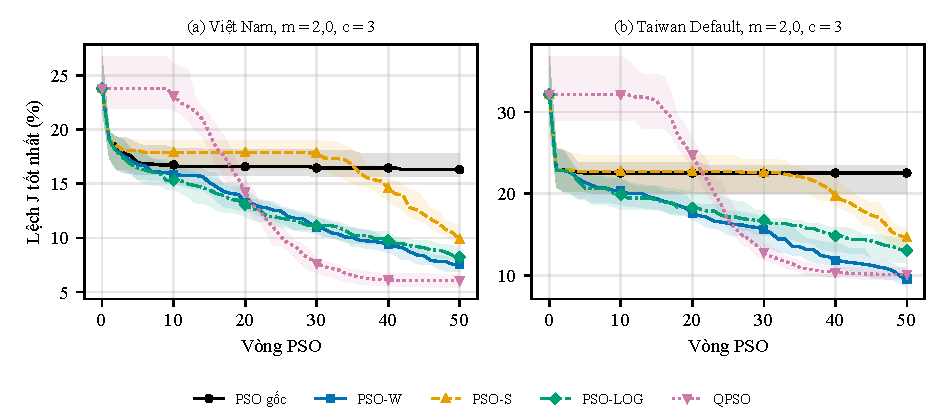
\includegraphics[width=\linewidth]{e7-quy-dao-gbest}
\caption{TN1: quỹ đạo gbest khi PSO tìm tâm (30 hạt, 50 vòng, $m = 2$, $c = 3$), đo bằng độ lệch $J_m$ của gbest so với $J_m$ tốt
nhất, theo vòng; đường là trung vị, dải màu là khoảng tứ phân vị qua 30 seed}
\label{fig:e7-quy-dao}
\end{figure}

Bảng~\ref{tab:e5-tong-hop} đặt 5 phiên bản (20 hạt, 30 vòng) cạnh 3 cách khởi tạo không dùng PSO. Trên 2 bộ chính với
$c = 3$, mọi tổ hợp PSO và mọi đối chứng,
kể cả FCM khởi tạo $U$ ngẫu nhiên, đạt $J$ tốt nhất ở mọi lượt; so theo seed với FCM k-means++, mọi lượt cho cùng $J_m$
(\soLieuENamVietNamCBaCungJKpp\% và \soLieuENamTaiwanKiemChungCBaCungJKpp\%), cùng PC và AUC, và số vòng FCM không giảm. Ở 3
cấu hình có nhiều cực tiểu, nhóm đếm số seed (trên 30) mà mỗi cách đạt cực tiểu tốt nhất. Trên Taiwan Default chưa log
($c = 6$), k-means++ đạt ở cả 30 seed (trượt \soLieuENamKhongLogDoiChungKppTruot), còn các tổ hợp PSO đạt ít hơn hoặc bằng
(tỉ lệ đạt của PSO trừ của k-means++ từ \soLieuENamKhongLogDoiChungHieuKppMin{} đến \soLieuENamKhongLogDoiChungHieuKppMax{} điểm
phần trăm). Trên Taiwan Default với $m = 1{,}5$, $c = 7$, k-means++ trượt
\soLieuEBayTaiwanKiemChungCBayDoiChungKppTruot/30 seed và mọi tổ hợp PSO đạt ít hơn k-means++
(\soLieuEBayTaiwanKiemChungCBayDoiChungHieuKppMin{} đến \soLieuEBayTaiwanKiemChungCBayDoiChungHieuKppMax{} điểm). Chỉ trên Việt
Nam với $m = 1{,}5$, $c = 8$, PSO đạt nhiều hơn k-means++ (k-means++ trượt \soLieuEBayVietNamCTamDoiChungKppTruot/30 seed, PSO
hơn \soLieuEBayVietNamCTamDoiChungHieuKppMin{} đến \soLieuEBayVietNamCTamDoiChungHieuKppMax{} điểm, tức 2--3 seed); mức chênh
này nhỏ và lấy lại được bằng cách chạy k-means++ nhiều lần (chạy lại 20 lần đạt cả 30 seed). So với FCM khởi tạo $U$ ngẫu nhiên, PSO có
tốt hơn trên Taiwan Default chưa log (FCM $U$ ngẫu nhiên chỉ đạt 57\%), đúng loại kết quả các bài báo ghi nhận; nhưng FCM khởi
tạo từ $c$ điểm dữ liệu ngẫu nhiên, tức bộ tâm của một hạt trước khi bay, đã đạt ở \soLieuENamKhongLogFcmDiemK/30 seed. Lợi
ích so với khởi tạo ngẫu nhiên vì vậy đến từ việc khởi tạo bằng tâm, không từ bước tìm kiếm của bầy. Trong khi đó PSO chậm hơn FCM k-means++ khoảng \soLieuENamTaiwanKiemChungCBaTiLeThoiGianTv{} lần trên Taiwan
Default và \soLieuENamVietNamCBaTiLeThoiGianTv{} lần trên Việt Nam (20 hạt, 30 vòng, trung vị).


\begin{table}[htbp]
\centering
\caption{TN1 -- PSO gốc và các phiên bản cải tiến làm bộ khởi tạo tâm cho FCM (20 hạt, 30 vòng, 30 seed)}
\label{tab:e5-tong-hop}
\footnotesize
\setlength{\tabcolsep}{3pt}
\begin{tabular}{@{}lrrrrrrrrr@{}}
\toprule
& \multicolumn{3}{c}{Việt Nam, c~=~3} & \multicolumn{3}{c}{Taiwan Default, c~=~3} & \multicolumn{3}{c}{Taiwan Default (không log), c~=~6} \\
\cmidrule(lr){2-4} \cmidrule(lr){5-7} \cmidrule(lr){8-10}
Phương pháp & \begin{tabular}[b]{@{}c@{}}Đạt\\(\%)\end{tabular} & \begin{tabular}[b]{@{}c@{}}Lệch\\(\%)\end{tabular} & \begin{tabular}[b]{@{}c@{}}Thời gian\\(s)\end{tabular} & \begin{tabular}[b]{@{}c@{}}Đạt\\(\%)\end{tabular} & \begin{tabular}[b]{@{}c@{}}Lệch\\(\%)\end{tabular} & \begin{tabular}[b]{@{}c@{}}Thời gian\\(s)\end{tabular} & \begin{tabular}[b]{@{}c@{}}Đạt\\(\%)\end{tabular} & \begin{tabular}[b]{@{}c@{}}Lệch\\(\%)\end{tabular} & \begin{tabular}[b]{@{}c@{}}Thời gian\\(s)\end{tabular} \\
\midrule
FCM (U ngẫu nhiên) & 100 & -- & 0,98 & 100 & -- & 0,06 & 57 & -- & 0,50 \\
FCM (điểm ngẫu nhiên) & 100 & 55,5 & 0,81 & 100 & 63,1 & 0,04 & 100 & 48,4 & 0,15 \\
FCM (k-means++) & 100 & -- & 0,88 & 100 & -- & 0,04 & 100 & -- & 0,14 \\
\midrule
PSO gốc (1995) & 100 & 17,6 & 1,65 & 100 & 23,2 & 0,97 & 93 & 21,3 & 1,61 \\
PSO-W (1998) & 100 & 10,0 & 1,48 & 100 & 13,8 & 1,30 & 100 & 17,9 & 1,85 \\
PSO-S (2022) & 100 & 13,6 & 0,94 & 100 & 17,7 & 0,80 & 100 & 20,1 & 1,64 \\
PSO-LOG (2022) & 100 & 11,8 & 1,32 & 100 & 16,2 & 0,74 & 97 & 19,1 & 1,55 \\
QPSO (2004) & 100 & 9,9 & 1,36 & 100 & 13,9 & 0,82 & 83 & 12,7 & 1,57 \\
\bottomrule
\end{tabular}
\par\smallskip\parbox{\linewidth}{\scriptsize Ghi chú: Đạt: tỉ lệ lượt đạt J tốt nhất sau khi FCM chạy tới hội tụ; lệch: J\textsubscript{m} của bộ tâm đưa vào FCM (gbest của PSO, hoặc c điểm ngẫu nhiên) so với J\textsubscript{m} tốt nhất (\%), trung vị; thời gian gồm PSO và FCM, trung vị. Bầy PSO khởi tạo bằng điểm dữ liệu ngẫu nhiên, chạy đủ số vòng, c\textsubscript{1} = c\textsubscript{2} = 2 (trừ QPSO).}
\end{table}


Các chỉ số phân cụm cũng không phân biệt được các cách khởi tạo (Bảng~\ref{tab:e5-chi-so}). Trên các lượt cho cùng nghiệm,
PC và AUC của mọi phương pháp chênh với FCM k-means++ dưới $10^{-4}$, Silhouette chênh nhiều nhất 0,018 trên 2 bộ chính.
XB thì dao động rất rộng giữa các phương pháp dù cùng nghiệm, vì 2 tâm gần trùng làm mẫu số gần bằng không
(mục~\ref{sec:chi-so}); tiểu luận vì vậy không dùng XB để so.
\label{sec:e5-chi-so}

\begin{table}[htbp]
\centering
\caption{TN1 -- chỉ số sau khi FCM hội tụ: FCM (k-means++) và mức chênh của các phương pháp còn lại}
\label{tab:e5-chi-so}
\footnotesize
\setlength{\tabcolsep}{3pt}
\begin{tabular}{@{}lrrrrrrr@{}}
\toprule
& \multicolumn{3}{c}{FCM (k-means++)} & \multicolumn{3}{c}{Chênh lớn nhất theo seed} & \\
\cmidrule(lr){2-4} \cmidrule(lr){5-7}
Cấu hình & PC & Silhouette & AUC & PC & AUC & Silhouette & XB (khoảng) \\
\midrule
Việt Nam, c = 3 & 0,373 & 0,080 & 0,840 & 8,14·10\textsuperscript{−6} & 8,88·10\textsuperscript{−6} & 0,001 & 3.677,89 -- 4.664,12 \\
Taiwan, c = 3 & 0,395 & 0,129 & 0,434 & 4,68·10\textsuperscript{−6} & 7,66·10\textsuperscript{−6} & 0,018 & 1,57·10\textsuperscript{9} -- 6,98·10\textsuperscript{9} \\
Taiwan chưa log, c = 6 & 0,196 & 0,054 & 0,545 & 3,15·10\textsuperscript{−6} & 2,74·10\textsuperscript{−5} & 0,116 & 3,33·10\textsuperscript{12} -- 3,60·10\textsuperscript{14} \\
\bottomrule
\end{tabular}
\par\smallskip\parbox{\linewidth}{\scriptsize Ghi chú: PC, Silhouette, AUC: trung vị 30 seed của FCM (k-means++); chênh lớn nhất: |hiệu| lớn nhất theo từng seed giữa một phương pháp bất kỳ (3 đối chứng, 45 tổ hợp PSO) và FCM (k-means++), chỉ trên các lượt cùng nghiệm; XB: khoảng trung vị của 8 phương pháp (3 đối chứng, 5 phiên bản PSO với 20 hạt, 30 vòng); XB không ổn định khi 2 tâm gần trùng, xem mục~\ref{sec:e5-chi-so}.}
\end{table}


\subsection{Giải thích: số cực tiểu của hàm mục tiêu}
\label{sec:vi-sao}

TN2 chạy FCM ($m = 2$) từ 30 khởi tạo độ thuộc ngẫu nhiên và 30 khởi tạo k-means++ trên mỗi bộ, mỗi $c$, rồi gom các $J_m$
cuối lệch nhau không quá $10^{-4}$ (tương đối) thành một mức; số mức là số cực tiểu \emph{quan sát được}, không phải phép chứng
minh $J_m$ chỉ có từng ấy cực tiểu. Một lượt là \emph{sụp} khi mọi tâm dồn về trung bình dữ liệu (độ lớn tâm dưới $10^{-3}$
trên dữ liệu z-score), tức mọi độ thuộc bằng $1/c$ (Bảng~\ref{tab:e3-chan-doan}).

\begin{table}[htbp]
\centering
\caption{TN2 -- chẩn đoán số cực tiểu của J\textsubscript{m}: FCM từ 30 khởi tạo mỗi kiểu}
\label{tab:e3-chan-doan}
\footnotesize
\setlength{\tabcolsep}{3pt}
\begin{tabular}{@{}lrrrrrrr@{}}
\toprule
& & \multicolumn{3}{c}{U ngẫu nhiên} & \multicolumn{3}{c}{k-means++} \\
\cmidrule(lr){3-5} \cmidrule(lr){6-8}
Bộ dữ liệu & c & \begin{tabular}[b]{@{}c@{}}Số\\cực tiểu\end{tabular} & \begin{tabular}[b]{@{}c@{}}Đạt J\\tốt nhất (\%)\end{tabular} & \begin{tabular}[b]{@{}c@{}}Sụp\\(\%)\end{tabular} & \begin{tabular}[b]{@{}c@{}}Số\\cực tiểu\end{tabular} & \begin{tabular}[b]{@{}c@{}}Đạt J\\tốt nhất (\%)\end{tabular} & \begin{tabular}[b]{@{}c@{}}Sụp\\(\%)\end{tabular} \\
\midrule
Việt Nam & 2 & 1 & 100 & 0 & 1 & 100 & 0 \\
Việt Nam & 3 & 1 & 100 & 0 & 1 & 100 & 0 \\
Việt Nam & 4 & 1 & 100 & 0 & 1 & 100 & 0 \\
Taiwan Default & 2 & 1 & 100 & 0 & 1 & 100 & 0 \\
Taiwan Default & 3 & 1 & 100 & 0 & 1 & 100 & 0 \\
Taiwan Default & 4 & 1 & 100 & 0 & 1 & 100 & 0 \\
Taiwan Default & 5 & 1 & 100 & 0 & 1 & 100 & 0 \\
Taiwan Default & 6 & 1 & 100 & 0 & 1 & 100 & 0 \\
Taiwan Default (không log) & 2 & 1 & 100 & 0 & 1 & 100 & 0 \\
Taiwan Default (không log) & 3 & 1 & 100 & 0 & 1 & 100 & 0 \\
Taiwan Default (không log) & 4 & 1 & 100 & 0 & 1 & 100 & 0 \\
Taiwan Default (không log) & 5 & 2 & 37 & 0 & 1 & 100 & 0 \\
Taiwan Default (không log) & 6 & 2 & 57 & 0 & 1 & 100 & 0 \\
South German Credit & 2 & 1 & 100 & 100 & 1 & 100 & 100 \\
South German Credit & 3 & 1 & 100 & 100 & 1 & 100 & 100 \\
South German Credit & 4 & 1 & 100 & 100 & 1 & 100 & 100 \\
German Credit (bản số) & 2 & 1 & 100 & 100 & 1 & 100 & 100 \\
German Credit (bản số) & 3 & 1 & 100 & 100 & 1 & 100 & 100 \\
German Credit (bản số) & 4 & 1 & 100 & 100 & 1 & 100 & 100 \\
Australian Credit & 2 & 1 & 100 & 100 & 1 & 100 & 100 \\
Australian Credit & 3 & 1 & 100 & 100 & 1 & 100 & 100 \\
Australian Credit & 4 & 1 & 100 & 100 & 1 & 100 & 100 \\
Polish Bankruptcy & 2 & 1 & 100 & 0 & 1 & 100 & 0 \\
Polish Bankruptcy & 3 & 1 & 100 & 0 & 1 & 100 & 0 \\
Polish Bankruptcy & 4 & 1 & 100 & 0 & 1 & 100 & 0 \\
Taiwan Bankruptcy & 2 & 1 & 100 & 100 & 1 & 100 & 100 \\
Taiwan Bankruptcy & 3 & 1 & 100 & 100 & 1 & 100 & 100 \\
Taiwan Bankruptcy & 4 & 1 & 100 & 100 & 2 & 90 & 90 \\
\bottomrule
\end{tabular}
\par\smallskip\parbox{\linewidth}{\scriptsize Ghi chú: số cực tiểu: số mức J\textsubscript{m} lệch nhau quá $10^{-4}$ (tương đối), kể cả mức sụp; đạt J tốt nhất so với J\textsubscript{m} nhỏ nhất của cả 2 kiểu; sụp: mọi tâm dồn về trung bình dữ liệu ($\max|V| < 10^{-3}$).}
\end{table}


Bảng cho thấy 3 nhóm hành vi. \emph{Một cực tiểu:} trên 2 bộ chính đã lấy log, ở mọi cấu hình đã thử, $J_m$ chỉ có
\soLieuEBaTaiwanKiemChungCSauUNgauNhienSoCucTieu{} cực tiểu và \soLieuEBaTaiwanKiemChungCSauUNgauNhienDatJ\% lượt đạt nó, với cả
2 kiểu khởi tạo; Polish Bankruptcy cũng vậy nhưng gần sụp (PC \soLieuEBaPolishCHaiUNgauNhienPc{} với $c = 2$). \emph{Sụp:}
South German, German bản số và Australian sụp ở \soLieuEBaSouthGermanCHaiUNgauNhienSup\% lượt với mọi $c$, Taiwan Bankruptcy
sụp \soLieuEBaTaiwanPhaSanCHaiUNgauNhienSup\% với khởi tạo ngẫu nhiên; khi mức thấp nhất là nghiệm sụp, một bộ khởi tạo tìm được
$J_m$ thấp hơn chỉ đưa FCM tới nghiệm sụp nhanh hơn. \emph{Nhiều cực tiểu không sụp:} chỉ Taiwan Default \emph{chưa lấy log}
với $c = 5, 6$ và khởi tạo ngẫu nhiên (\soLieuEBaTaiwanKiemChungKhongLogCSauUNgauNhienDatJ\% lượt đạt cực tiểu tốt hơn với
$c = 6$); ngay ở đây k-means++ đạt cực tiểu tốt hơn ở \soLieuEBaTaiwanKiemChungKhongLogCSauKmeansPpDatJ\% lượt, và sau khi lấy
log chỉ còn 1 cực tiểu.

TN2 còn quét 2 bộ chính với $m \in \{1{,}5;\ 2\}$, $c = 2, \dots, 8$ và 4 kiểu khởi tạo, gồm cả PSO-W
(Bảng~\ref{tab:e6-cuc-tieu}). $J_m$ chỉ có 1 cực tiểu quan sát được ở \soLieuESauSoCauHinhMotCucTieu{} trên
\soLieuESauSoCauHinh{} cấu hình; 2 cấu hình còn lại có $m = 1{,}5$ và nhiều cụm (Taiwan Default $c = 7$, Việt Nam $c = 8$).
Cột khoảng cách nhỏ nhất giữa 2 tâm cho thấy với $m = 2$ và $c \ge 3$ 2 tâm gần trùng nhau
(\soLieuESauVietNamMHaiPhayKhongCBaKcTam{} trên Việt Nam với $c = 3$), tức FCM thực chất tìm được ít cụm hơn số cụm yêu cầu.

\begin{table}[htbp]
\centering
\caption{TN2 -- số cực tiểu của J\textsubscript{m} và tỉ lệ đạt J tốt nhất theo m, c và kiểu khởi tạo}
\label{tab:e6-cuc-tieu}
\footnotesize
\setlength{\tabcolsep}{3pt}
\begin{tabular}{@{}lrrrrrrrrr@{}}
\toprule
Bộ, m & c & \begin{tabular}[b]{@{}c@{}}Số\\cực tiểu\end{tabular} & \begin{tabular}[b]{@{}c@{}}U ngẫu\\nhiên\end{tabular} & \begin{tabular}[b]{@{}c@{}}Điểm\\ngẫu nhiên\end{tabular} & \begin{tabular}[b]{@{}c@{}}k-\\means++\end{tabular} & \begin{tabular}[b]{@{}c@{}}PSO-W\\\end{tabular} & \begin{tabular}[b]{@{}c@{}}Sụp\\(\%)\end{tabular} & \begin{tabular}[b]{@{}c@{}}K/c tâm\\nhỏ nhất\end{tabular} & AUC \\
\midrule
Taiwan Default, m = 1,5 & 2 & 1 & 100 & 100 & 100 & 100 & 0 & 5,07 & 0,446 \\
 & 3 & 1 & 100 & 100 & 100 & 100 & 0 & 0,99 & 0,639 \\
 & 4 & 1 & 100 & 100 & 100 & 100 & 0 & 1,45 & 0,664 \\
 & 5 & 1 & 100 & 100 & 100 & 100 & 0 & 1,00 & 0,694 \\
 & 6 & 1 & 100 & 100 & 100 & 100 & 0 & 0,85 & 0,707 \\
 & 7 & 4 & 63 & 83 & 93 & 77 & 0 & 0,98 & 0,707 \\
 & 8 & 1 & 100 & 100 & 100 & 100 & 0 & 4,83·10\textsuperscript{−5} & 0,709 \\
\midrule
Taiwan Default, m = 2,0 & 2 & 1 & 100 & 100 & 100 & 100 & 0 & 3,28 & 0,451 \\
 & 3 & 1 & 100 & 100 & 100 & 100 & 0 & 5,79·10\textsuperscript{−5} & 0,434 \\
 & 4 & 1 & 100 & 100 & 100 & 100 & 0 & 1,58·10\textsuperscript{−5} & 0,423 \\
 & 5 & 1 & 100 & 100 & 100 & 100 & 0 & 2,05·10\textsuperscript{−6} & 0,417 \\
 & 6 & 1 & 100 & 100 & 100 & 100 & 0 & 3,06·10\textsuperscript{−7} & 0,414 \\
 & 7 & 1 & 100 & 100 & 100 & 100 & 0 & 5,30·10\textsuperscript{−10} & 0,412 \\
 & 8 & 1 & 100 & 100 & 100 & 100 & 0 & 3,89·10\textsuperscript{−11} & 0,449 \\
\midrule
Việt Nam, m = 1,5 & 2 & 1 & 100 & 100 & 100 & 100 & 0 & 4,15 & 0,836 \\
 & 3 & 1 & 100 & 100 & 100 & 100 & 0 & 2,58 & 0,903 \\
 & 4 & 1 & 100 & 100 & 100 & 100 & 0 & 2,40 & 0,925 \\
 & 5 & 1 & 100 & 100 & 100 & 100 & 0 & 2,19 & 0,950 \\
 & 6 & 1 & 100 & 100 & 100 & 100 & 0 & 1,30 & 0,950 \\
 & 7 & 1 & 100 & 100 & 100 & 100 & 0 & 1,65 & 0,950 \\
 & 8 & 2 & 100 & 93 & 90 & 97 & 0 & 1,09 & 0,950 \\
\midrule
Việt Nam, m = 2,0 & 2 & 1 & 100 & 100 & 100 & 100 & 0 & 2,68 & 0,784 \\
 & 3 & 1 & 100 & 100 & 100 & 100 & 0 & 0,04 & 0,840 \\
 & 4 & 1 & 100 & 100 & 100 & 100 & 0 & 4,97·10\textsuperscript{−3} & 0,866 \\
 & 5 & 1 & 100 & 100 & 100 & 100 & 0 & 4,71·10\textsuperscript{−5} & 0,879 \\
 & 6 & 1 & 100 & 100 & 100 & 100 & 0 & 1,90·10\textsuperscript{−4} & 0,886 \\
 & 7 & 1 & 100 & 100 & 100 & 100 & 0 & 1,46·10\textsuperscript{−5} & 0,888 \\
 & 8 & 1 & 100 & 100 & 100 & 100 & 0 & 3,45·10\textsuperscript{−11} & 0,867 \\
\bottomrule
\end{tabular}
\par\smallskip\parbox{\linewidth}{\scriptsize Ghi chú: 30 seed mỗi kiểu khởi tạo; số cực tiểu: số mức J\textsubscript{m} lệch nhau quá $10^{-4}$ (tương đối) trên 120 lượt; 4 cột kiểu khởi tạo: tỉ lệ lượt (\%) có J\textsubscript{m} $\le (1 + 10^{-4})$ lần mức thấp nhất; K/c tâm nhỏ nhất: khoảng cách nhỏ nhất giữa 2 tâm (dữ liệu z-score), trung vị; AUC: AUC tách rủi ro, trung vị. PSO-W: 20 hạt, 30 vòng.}
\end{table}


\subsection{Nhận xét và lý do chuyển sang tìm trọng số}
\label{sec:chuyen-huong}

Kết quả của hướng ban đầu trả lời CH1 và khớp với TN2: khi $J_m$ chỉ có 1 cực tiểu, PSO và FCM làm giảm cùng một hàm nên PSO
không còn gì để tìm; ở các cấu hình hiếm hoi có nhiều cực tiểu, chạy lại k-means++ vài lần là đủ. Hai giới hạn cần đọc kèm:
các cấu hình nhiều cực tiểu được chọn bằng TN2 trên chính mẫu kiểm chứng (thiên lệch nghiêng về phía có lợi cho PSO, nên không
làm yếu kết luận âm), và với 30 seed chỉ khác biệt lớn mới phát hiện được.

Như đã tổng hợp ở mục~\ref{sec:trai-chieu}, các bài đề xuất PSO--FCM báo phương pháp của mình
tốt hơn FCM nhưng với đối chứng không tương đương: bài 02 khởi tạo FCM ngẫu nhiên còn PSO--FCM khởi tạo bằng đồ
thị~\cite{qian2022psofcm}, bài 04 không có FCM thuần làm đối chứng~\cite{zhang2025qpsofcm}. Khi FCM được so trong điều kiện
tương đương, các nghiên cứu độc lập cho kết quả giống của nhóm: hoà trên dữ liệu dễ~\cite{mehdizadeh2008hybrid}, thua hoặc
không hơn và chậm hơn nhiều lần~\cite{ghamisi2015swarm,omran2004thesis,izakian2009hybrid}, kể cả bản PSO--FCM đối chứng trong
bài 06~\cite{liu2021msgwo}; và Hathaway và Bezdek đã ghi nhận từ năm 1988 rằng trong thực tế FCM khá ít phụ thuộc khởi
tạo~\cite{hathaway1988recent}. Tài liệu vì vậy không cho lý do để kỳ vọng PSO tìm tâm cải thiện FCM trên dữ liệu như của nhóm.

Cùng tài liệu đó gợi ý hướng khác: ở bài 06, đánh trọng số thuộc tính đóng góp nhiều hơn hẳn phần tìm tâm bằng bầy
sói~\cite{liu2021msgwo} (mục~\ref{sec:cac-nghien-cuu}), trong khi FCM không tự chọn được
trọng số (mục~\ref{sec:kc-trong-so}). Nhóm vì vậy giữ nguyên dữ liệu, tiền xử lý, 5 phiên bản PSO và cách kiểm định, chỉ đổi
thứ PSO tối ưu: từ tâm cụm sang trọng số thuộc tính. Các mục sau trình bày kết quả của hướng mới.

% Giang
\section{PSO tìm trọng số so với các đối chứng}
\label{sec:pso-trong-so}

Mục này trả lời CH2 bằng TN3: PSO-W tìm trọng số thuộc tính cho FCM (mục~\ref{sec:pso-trong-so-pp}), so với FCM k-means++,
WFCM trọng số giải tích và tìm ngẫu nhiên cùng 500 lần tính fitness, trên 7 bộ tín dụng với $c = 2, 3, 4$ và $m = 2$
(\soLieuETamSoLuot{} lượt, không lượt nào lỗi). Hai chỉ số chính được chốt trước khi chạy là AUC phân hoạch và chênh tỉ lệ vỡ
nợ $\Delta r$ (mục~\ref{sec:chi-so}); cả hai dùng nhãn, còn nhãn không đi vào fitness. Silhouette chỉ là chỉ số phụ vì chính
nó là fitness. Mỗi cặp (PSO, đối chứng) được so theo cặp seed bằng Wilcoxon ở từng bộ, từng $c$ và từng chỉ số, hiệu chỉnh
Holm trên cả \soLieuETamSoPhep{} phép thử (Bảng~\ref{tab:e8-ket-qua}, \ref{tab:e8-tong-hop}).

\begin{table}[htbp]
\centering
\caption{TN3 -- PSO tìm trọng số thuộc tính so với 3 đối chứng trên 7 bộ dữ liệu tín dụng}
\label{tab:e8-ket-qua}
\footnotesize
\setlength{\tabcolsep}{3pt}
\begin{tabular}{@{}llrrrrrrrr@{}}
\toprule
& & \multicolumn{4}{c}{AUC phân hoạch} & \multicolumn{4}{c}{Chênh tỉ lệ vỡ nợ} \\
\cmidrule(lr){3-6} \cmidrule(lr){7-10}
Bộ dữ liệu & c & FCM & WFCM & NN & PSO & FCM & WFCM & NN & PSO \\
\midrule
Việt Nam & 2 & 0,799\textsuperscript{+} & 0,816\textsuperscript{+} & 0,840\textsuperscript{+} & \textbf{0,850} & 0,284\textsuperscript{+} & 0,313\textsuperscript{+} & 0,356\textsuperscript{+} & \textbf{0,438} \\
 & 3 & 0,834\textsuperscript{+} & \textbf{0,860\textsuperscript{--}} & 0,843 & 0,844 & 0,341\textsuperscript{+} & \textbf{0,478} & 0,415\textsuperscript{+} & 0,465 \\
 & 4 & 0,863\textsuperscript{+} & 0,871 & 0,870 & \textbf{0,876} & 0,420\textsuperscript{+} & \textbf{0,618} & 0,498\textsuperscript{+} & 0,557 \\
\midrule
Taiwan Default & 2 & \textbf{0,523\textsuperscript{--}} & 0,511 & 0,505\textsuperscript{+} & 0,517 & \textbf{0,036} & 0,019\textsuperscript{+} & 0,009\textsuperscript{+} & 0,033 \\
 & 3 & 0,601\textsuperscript{+} & 0,510\textsuperscript{+} & 0,655 & \textbf{0,664} & 0,155\textsuperscript{+} & 0,014\textsuperscript{+} & 0,238 & \textbf{0,261} \\
 & 4 & 0,526\textsuperscript{+} & 0,633 & \textbf{0,649} & 0,645 & 0,168\textsuperscript{+} & 0,235\textsuperscript{+} & 0,266 & \textbf{0,315} \\
\midrule
Polish Bankruptcy & 2 & \textbf{0,664\textsuperscript{--}} & \textbf{0,664\textsuperscript{--}} & 0,651 & 0,639 & \textbf{0,059\textsuperscript{--}} & \textbf{0,059\textsuperscript{--}} & 0,055 & 0,051 \\
 & 3 & \textbf{0,678} & 0,677 & 0,675 & 0,673 & 0,064 & 0,064 & \textbf{0,065} & 0,064 \\
 & 4 & 0,673 & 0,677 & \textbf{0,684} & 0,675 & 0,063 & 0,064 & 0,072 & \textbf{0,074} \\
\midrule
Taiwan Bankruptcy & 2 & \textbf{0,731\textsuperscript{--}} & \textbf{0,731} & 0,723 & 0,722 & \textbf{0,058\textsuperscript{--}} & \textbf{0,058} & 0,056 & 0,056 \\
 & 3 & 0,731 & 0,731 & \textbf{0,744} & 0,732 & 0,058 & 0,058 & \textbf{0,061} & 0,059 \\
 & 4 & \textbf{0,731} & \textbf{0,731} & \textbf{0,731} & 0,725 & 0,058 & 0,058 & \textbf{0,060} & 0,058 \\
\midrule
South German Credit & 2 & \textbf{0,525\textsuperscript{--}} & \textbf{0,525\textsuperscript{--}} & 0,516 & 0,507 & \textbf{0,042\textsuperscript{--}} & \textbf{0,042\textsuperscript{--}} & 0,028 & 0,013 \\
 & 3 & 0,529\textsuperscript{+} & 0,529\textsuperscript{+} & \textbf{0,612} & 0,610 & 0,207 & 0,211 & \textbf{0,261} & 0,256 \\
 & 4 & 0,530\textsuperscript{+} & 0,529\textsuperscript{+} & 0,625 & \textbf{0,630} & 0,255 & \textbf{0,312} & 0,279 & 0,286 \\
\midrule
German Credit (bản số) & 2 & 0,537 & 0,534 & \textbf{0,572\textsuperscript{--}} & 0,570 & 0,062 & 0,057 & \textbf{0,142\textsuperscript{--}} & 0,137 \\
 & 3 & \textbf{0,584} & 0,580 & 0,574 & 0,568 & \textbf{0,223} & 0,214 & 0,163 & 0,153 \\
 & 4 & \textbf{0,601} & 0,600 & 0,577 & 0,580 & \textbf{0,272} & 0,262 & 0,188 & 0,192 \\
\midrule
Australian Credit & 2 & \textbf{0,832\textsuperscript{--}} & \textbf{0,832\textsuperscript{--}} & 0,822 & 0,816 & \textbf{0,666\textsuperscript{--}} & \textbf{0,666\textsuperscript{--}} & 0,656 & 0,646 \\
 & 3 & \textbf{0,832} & \textbf{0,832} & 0,779 & 0,791 & \textbf{0,666} & \textbf{0,666} & 0,559 & 0,589 \\
 & 4 & 0,832 & 0,832 & \textbf{0,875} & 0,836 & 0,666 & 0,666 & \textbf{0,764} & 0,685 \\
\bottomrule
\end{tabular}
\par\smallskip\parbox{\linewidth}{\scriptsize Ghi chú: Trung vị 30 seed, m = 2. FCM: FCM k-means++; WFCM: trọng số giải tích; NN: tìm ngẫu nhiên trọng số. Đậm: cao nhất hàng. Dấu \textsuperscript{+} / \textsuperscript{--} sau một đối chứng: PSO tốt hơn / kém hơn đối chứng đó có ý nghĩa (Wilcoxon theo cặp seed, Holm toàn họ, $\alpha = 0{,}05$); không dấu: không khác có ý nghĩa.}
\end{table}


\begin{table}[htbp]
\centering
\caption{TN3 -- số cấu hình PSO tìm trọng số tốt hơn / không khác / kém hơn từng đối chứng}
\label{tab:e8-tong-hop}
\footnotesize
\setlength{\tabcolsep}{3pt}
\begin{tabular}{@{}lccc@{}}
\toprule
PSO so với & FCM & WFCM giải tích & Ngẫu nhiên \\
\midrule
AUC phân hoạch & 7 / 9 / 5 & 4 / 13 / 4 & 2 / 18 / 1 \\
Chênh tỉ lệ vỡ nợ & 5 / 12 / 4 & 4 / 14 / 3 & 4 / 16 / 1 \\
Silhouette & 15 / 4 / 2 & 15 / 3 / 3 & 12 / 9 / 0 \\
\midrule
Thời gian trung vị (giây) & 0,05 & 0,24 & 39,87 \\
Thời gian PSO (giây) & \multicolumn{3}{c}{29,2} \\
\bottomrule
\end{tabular}
\par\smallskip\parbox{\linewidth}{\scriptsize Ghi chú: 21 cấu hình (7 bộ × 3 số cụm), Wilcoxon theo cặp seed, Holm toàn họ, $\alpha = 0{,}05$. Silhouette là fitness của PSO nên chỉ là chỉ số phụ.}
\end{table}


\subsection{Tách rủi ro trên 2 bộ chính}

Trên Việt Nam, PSO tốt hơn FCM thường có ý nghĩa ở cả 3 số cụm, cả về AUC phân
hoạch lẫn chênh tỉ lệ vỡ nợ. Với $c = 2$, AUC tăng từ \soLieuETamVietNamCHaiFcmKppAucCung{} lên
\soLieuETamVietNamCHaiPsoTrongSoAucCung{} và $\Delta r$ từ \soLieuETamVietNamCHaiFcmKppChenhTiLe{} lên
\soLieuETamVietNamCHaiPsoTrongSoChenhTiLe; với $c = 4$, $\Delta r$ tăng từ \soLieuETamVietNamCBonFcmKppChenhTiLe{} lên
\soLieuETamVietNamCBonPsoTrongSoChenhTiLe. Trên Taiwan Default với $c = 3$, AUC tăng từ
\soLieuETamTaiwanKiemChungCBaFcmKppAucCung{} lên \soLieuETamTaiwanKiemChungCBaPsoTrongSoAucCung{} và $\Delta r$ từ
\soLieuETamTaiwanKiemChungCBaFcmKppChenhTiLe{} lên \soLieuETamTaiwanKiemChungCBaPsoTrongSoChenhTiLe; $c = 4$ cho kết quả cùng
chiều. Ở vai trò tìm tâm, PSO không làm được điều này vì cho cùng nghiệm với FCM ở mọi lượt (mục~\ref{sec:e5-dat-j}).

\subsection{Phần do cơ chế bầy đàn và so với trọng số bằng công thức}

So với tìm ngẫu nhiên cùng ngân sách, PSO cho fitness tốt hơn có ý nghĩa ở
\soLieuETamSilhouetteNgauNhienTrongSoHon{} trên \soLieuETamSoCauHinh{} cấu hình và không kém ở cấu hình nào. Hình~\ref{fig:e8-hoi-tu}
cho thấy khoảng cách hình thành trong khoảng 50 tới 100 lần tính fitness đầu: sau đó tìm ngẫu nhiên gần như ngừng cải thiện,
còn PSO tiếp tục tăng tới khoảng 200 lần trên Việt Nam và tới cuối ngân sách trên Taiwan Default. Về 2 chỉ số chính, PSO tốt hơn tìm ngẫu nhiên ở \soLieuETamChenhTiLeNgauNhienTrongSoHon{} cấu hình theo $\Delta r$
(3 cấu hình của Việt Nam và Taiwan Default $c = 2$) và \soLieuETamAucCungNgauNhienTrongSoHon{} cấu hình theo AUC; ở phần
lớn cấu hình còn lại 2 cách không khác nhau. Như vậy trên Việt Nam, một phần lợi ích về tách rủi ro đến từ chính cơ chế bầy
đàn; ở các bộ khác, lợi ích (nếu có) chủ yếu đến từ việc đánh trọng số theo Silhouette, và tìm ngẫu nhiên đủ nhiều cũng đạt
được.

\begin{figure}[htbp]
\centering
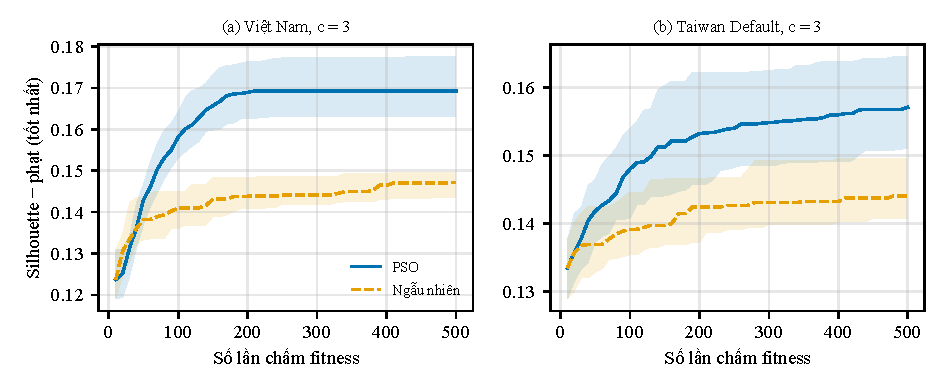
\includegraphics[width=\linewidth]{e8-hoi-tu}
\caption{TN3: fitness tốt nhất (Silhouette trừ phạt cụm nhỏ) theo số lần tính fitness của PSO và tìm ngẫu nhiên; đường là
trung vị, dải là khoảng tứ phân vị của 30 seed}
\label{fig:e8-hoi-tu}
\end{figure}

WFCM giải tích rẻ hơn khoảng hai bậc độ lớn và trên Việt Nam với $c = 3$,
$c = 4$ cho AUC và $\Delta r$ ngang hoặc hơn PSO. Nhưng trên Taiwan Default với $c = 3$, công thức gần như làm mất khả năng
tách rủi ro (AUC \soLieuETamTaiwanKiemChungCBaWfcmGiaiTichAucCung, $\Delta r$
\soLieuETamTaiwanKiemChungCBaWfcmGiaiTichChenhTiLe), trong khi PSO đạt \soLieuETamTaiwanKiemChungCBaPsoTrongSoAucCung{} và
\soLieuETamTaiwanKiemChungCBaPsoTrongSoChenhTiLe. Công thức dồn trọng số vào thuộc tính làm các cụm chặt nhất; trên Taiwan
Default đó là dư nợ các tháng (BILL\_AMT2--6, seed 1000), đúng nhóm mà PSO giảm trọng số (Hình~\ref{fig:e8-trong-so}). Tính
trên cả 7 bộ, PSO tốt hơn WFCM giải tích ở \soLieuETamAucCungWfcmGiaiTichHon{} cấu hình và kém ở
\soLieuETamAucCungWfcmGiaiTichKem{} cấu hình theo AUC; không cách nào thắng ở mọi bộ.

Các đối chứng trên đều là FCM với $m = 2$, mà với $c \ge 3$ FCM này gần suy biến (mục~\ref{sec:vi-sao}). Vì vậy nhóm chạy
thêm K-means không trọng số, cùng seed và tiền xử lý, làm mốc tham chiếu (Bảng~\ref{tab:e8-kmeans}; Holm riêng trên
\soLieuETamKmSoPhep{} phép so để không đổi họ kiểm định của TN3). Với 2 cụm, PSO tốt hơn K-means trên cả 2 bộ chính. Với
3 và 4 cụm, K-means tách rủi ro tốt hơn: trên Việt Nam, $\Delta r$ với $c = 4$ là \soLieuETamKmVietNamCBonChenhTiLe{} so
với \soLieuETamVietNamCBonPsoTrongSoChenhTiLe{} của PSO; trên Taiwan Default, K-means hơn có ý nghĩa ở $\Delta r$ với $c = 4$,
còn với $c = 3$ không phát hiện khác biệt. Tính trên 7 bộ, PSO tốt hơn / không khác / kém K-means ở
\soLieuETamKmChenhTiLeHon{} / \soLieuETamKmChenhTiLeBang{} / \soLieuETamKmChenhTiLeKem{} cấu hình theo $\Delta r$. Như vậy lợi
ích của PSO tìm trọng số là lợi ích so với FCM $m = 2$, chưa phải so với mọi cách phân cụm; khi chỉ cần phân hoạch cứng,
K-means là mốc phải so trước. Lý do giữ FCM nằm ở độ thuộc (mục~\ref{sec:dien-giai}).

\begin{table}[htbp]
\centering
\caption{TN3 -- K-means không trọng số làm mốc tham chiếu trên 2 bộ chính}
\label{tab:e8-kmeans}
\footnotesize
\setlength{\tabcolsep}{3pt}
\begin{tabular}{@{}llrrrrrr@{}}
\toprule
& & \multicolumn{3}{c}{AUC phân hoạch} & \multicolumn{3}{c}{Chênh tỉ lệ vỡ nợ} \\
\cmidrule(lr){3-5} \cmidrule(lr){6-8}
Bộ dữ liệu & c & FCM & K-means & PSO & FCM & K-means & PSO \\
\midrule
Việt Nam & 2 & 0,799 & 0,843 & 0,850\textsuperscript{+} & 0,284 & 0,373 & 0,438\textsuperscript{+} \\
 & 3 & 0,834 & 0,879 & 0,844\textsuperscript{--} & 0,341 & 0,563 & 0,465\textsuperscript{--} \\
 & 4 & 0,863 & 0,882 & 0,876\textsuperscript{--} & 0,420 & 0,842 & 0,557\textsuperscript{--} \\
\midrule
Taiwan Default & 2 & 0,523 & 0,504 & 0,517\textsuperscript{+} & 0,036 & 0,007 & 0,033\textsuperscript{+} \\
 & 3 & 0,601 & 0,699 & 0,664 & 0,155 & 0,385 & 0,261 \\
 & 4 & 0,526 & 0,684 & 0,645 & 0,168 & 0,446 & 0,315\textsuperscript{--} \\
\bottomrule
\end{tabular}
\par\smallskip\parbox{\linewidth}{\scriptsize Ghi chú: Trung vị 30 seed, cùng seed và tiền xử lý với Bảng~\ref{tab:e8-ket-qua}. FCM: FCM k-means++, m = 2; PSO: FCM với trọng số do PSO tìm. Dấu \textsuperscript{+} / \textsuperscript{--}: PSO tốt hơn / kém hơn K-means có ý nghĩa (Wilcoxon theo cặp seed, Holm trên 42 phép so với K-means ở 7 bộ, $\alpha = 0{,}05$).}
\end{table}


\subsection{Trọng số tìm được và chi phí}

Hình~\ref{fig:e8-trong-so} cho thấy PSO chọn các thuộc tính có nghĩa kinh tế rõ. Trên Taiwan
Default, 3 thuộc tính nặng nhất là \soLieuETamTaiwanKiemChungTrongSoCaoMotTen, \soLieuETamTaiwanKiemChungTrongSoCaoHaiTen{} và
\soLieuETamTaiwanKiemChungTrongSoCaoBaTen{} (tình trạng trả nợ các tháng), trùng với trục phân cụm đọc được ở
mục~\ref{sec:dien-giai}, còn hạn mức và dư nợ các tháng bị giảm trọng số. Trên Việt Nam, trọng số dồn vào các tỉ số định giá
(\soLieuETamVietNamTrongSoCaoMotTen: EV/doanh thu; \soLieuETamVietNamTrongSoCaoBaTen: P/S) và đòn bẩy
(\soLieuETamVietNamTrongSoCaoHaiTen: tổng nợ/vốn chủ sở hữu), mỗi thuộc tính nặng gấp khoảng
\soLieuETamVietNamTrongSoCaoMotGiaTri{} lần trung bình, còn các tỉ số thanh khoản (X1, X2) và phần lớn tỉ số thị trường khác
bị đẩy về gần cận dưới. Vector trọng số vì vậy còn cho biết nhóm chỉ tiêu nào quyết định phân khúc.

\begin{figure}[htbp]
\centering
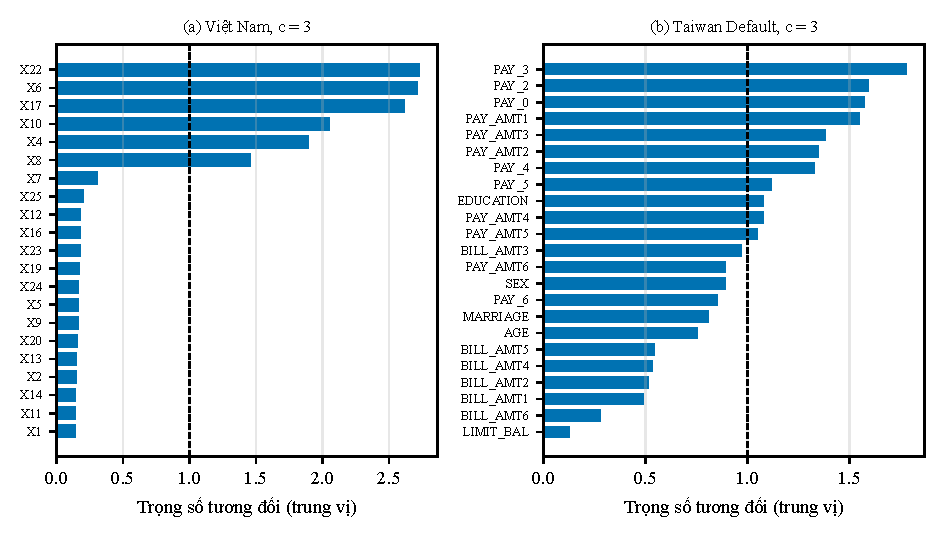
\includegraphics[width=\linewidth]{e8-trong-so}
\caption{TN3: trọng số tương đối (chia cho trung bình, trung vị của 30 seed) do PSO tìm với $c = 3$; đường đứt là trọng số
bằng nhau của FCM thường}
\label{fig:e8-trong-so}
\end{figure}

Một lượt PSO tìm trọng số mất khoảng \soLieuETamThoiGianPso{} giây (trung vị trên mọi cấu hình), so với
\soLieuETamThoiGianFcm{} giây của FCM thường, vì mỗi lần tính fitness là một lần chạy FCM và một lần tính Silhouette. Chi phí
này chỉ trả một lần khi dựng phân khúc, nên chấp nhận được với dữ liệu cỡ vài nghìn khách hàng; với dữ liệu lớn hơn cần giảm
mẫu Silhouette hoặc trần vòng FCM bên trong.


% Hà; Hải — QPSO và chi phí
\section{Năm phiên bản PSO khi tìm trọng số}
\label{sec:phien-ban-trong-so}

Mục này trả lời CH3 bằng TN4: 5 phiên bản PSO (Bảng~\ref{tab:ch2-phien-ban}) lắp vào cùng khung tìm trọng số
(Thuật toán~\ref{alg:pso-trong-so}), chạy trên 2 bộ chính với $c = 2, 3, 4$ ở 2 ngân sách, 500 lần tính fitness (10 hạt) và
1.000 lần (20 hạt), cùng 49 vòng (\soLieuEChinSoLuot{} lượt). Mỗi phiên bản được so với tìm ngẫu nhiên cùng ngân sách và mỗi
bản cải tiến được so với PSO gốc, trên điểm fitness (Silhouette trừ phạt), AUC phân hoạch và chênh tỉ lệ vỡ nợ, ở
\soLieuEChinSoO{} ô (2 bộ, 3 số cụm, 2 ngân sách); Holm hiệu chỉnh trên cả \soLieuEChinSoPhep{} phép so
(Bảng~\ref{tab:e9-tong-hop}--\ref{tab:e9-chenh}, Hình~\ref{fig:e9-quy-dao}).

\begin{table}[htbp]
\centering
\caption{TN4 -- số ô mỗi phiên bản tốt hơn / không khác / kém hơn tìm ngẫu nhiên và PSO gốc}
\label{tab:e9-tong-hop}
\footnotesize
\setlength{\tabcolsep}{3pt}
\begin{tabular}{@{}lcccccc@{}}
\toprule
& \multicolumn{3}{c}{So với tìm ngẫu nhiên} & \multicolumn{3}{c}{So với PSO gốc} \\
\cmidrule(lr){2-4} \cmidrule(lr){5-7}
Phiên bản & Điểm & AUC & $\Delta r$ & Điểm & AUC & $\Delta r$ \\
\midrule
Gốc & 11/1/0 & 2/10/0 & 9/3/0 & -- & -- & -- \\
W & 11/1/0 & 3/9/0 & 8/4/0 & 0/12/0 & 0/12/0 & 0/12/0 \\
S & 12/0/0 & 1/11/0 & 8/4/0 & 0/12/0 & 0/12/0 & 0/12/0 \\
LOG & 11/1/0 & 3/9/0 & 8/4/0 & 0/12/0 & 0/12/0 & 0/12/0 \\
QPSO & 12/0/0 & 4/8/0 & 9/3/0 & 0/12/0 & 0/12/0 & 0/12/0 \\
\bottomrule
\end{tabular}
\par\smallskip\parbox{\linewidth}{\scriptsize Ghi chú: 12 ô (2 bộ × 3 số cụm × 2 ngân sách). Điểm: Silhouette − phạt (chính là fitness); Wilcoxon theo cặp seed, Holm toàn họ, $\alpha = 0{,}05$.}
\end{table}


\subsection{Mọi phiên bản đều hơn tìm ngẫu nhiên}

Cả 5 phiên bản cho điểm fitness tốt hơn tìm ngẫu nhiên cùng ngân sách có ý nghĩa ở \soLieuEChinGocNgauNhienDiemHon{} đến
12 trên \soLieuEChinSoO{} ô, và chênh tỉ lệ vỡ nợ tốt hơn ở 8 đến 9 ô; không phiên bản nào kém tìm ngẫu nhiên ở ô nào, trên
chỉ số nào. Với AUC phân hoạch, phần lớn ô không khác (Bảng~\ref{tab:e9-tong-hop}): trên Việt Nam, mọi cách đánh trọng số đều
đã nâng AUC so với FCM thường, và khác biệt giữa PSO và tìm ngẫu nhiên nằm ở mức tách của cụm rủi ro cao, tức $\Delta r$. Hình~\ref{fig:e9-quy-dao}
cho thấy cách khoảng cách hình thành: mọi phiên bản tăng nhanh trong 200--400 lần tính fitness đầu rồi chững lại, còn tìm ngẫu
nhiên chỉ tăng chậm sau khoảng 200 lần. Theo trung vị, PSO với 500 lần đã có điểm cao hơn tìm ngẫu nhiên với 1.000 lần ở mọi ô;
chẳng hạn trên Việt
Nam với $c = 3$, điểm của PSO-W với 500 lần là \soLieuEChinVietNamCBaPsoWNamKhongKhongDiem{} so với
\soLieuEChinVietNamCBaNgauNhienMotKhongKhongKhongDiem{} của tìm ngẫu nhiên với 1.000 lần. Kết quả này củng cố TN3: phần lợi ích
do cơ chế bầy đàn không phụ thuộc phiên bản PSO nào được chọn.

\begin{table}[htbp]
\centering
\caption{TN4 -- Silhouette − phạt của 5 phiên bản PSO khi tìm trọng số thuộc tính}
\label{tab:e9-diem}
\footnotesize
\setlength{\tabcolsep}{3pt}
\begin{tabular}{@{}lllrrrrrrr@{}}
\toprule
Bộ dữ liệu & c & Ngân sách & FCM & NN & Gốc & W & S & LOG & QPSO \\
\midrule
Việt Nam & 2 & 500 & -- & 0,260 & 0,293\textsuperscript{+} & \textbf{0,296\textsuperscript{+}} & 0,292\textsuperscript{+} & \textbf{0,296\textsuperscript{+}} & 0,295\textsuperscript{+} \\
 &  & 1.000 &  & 0,263 & 0,296\textsuperscript{+} & 0,298\textsuperscript{+} & 0,295\textsuperscript{+} & 0,294\textsuperscript{+} & \textbf{0,303\textsuperscript{+}} \\
 & 3 & 500 & -- & 0,147 & 0,167\textsuperscript{+} & 0,169\textsuperscript{+} & 0,169\textsuperscript{+} & 0,170\textsuperscript{+} & \textbf{0,172\textsuperscript{+}} \\
 &  & 1.000 &  & 0,148 & 0,177\textsuperscript{+} & 0,175\textsuperscript{+} & 0,176\textsuperscript{+} & \textbf{0,180\textsuperscript{+}} & \textbf{0,180\textsuperscript{+}} \\
 & 4 & 500 & -- & 0,104 & 0,132\textsuperscript{+} & 0,133\textsuperscript{+} & 0,130\textsuperscript{+} & \textbf{0,135\textsuperscript{+}} & 0,130\textsuperscript{+} \\
 &  & 1.000 &  & 0,106 & 0,131\textsuperscript{+} & 0,134\textsuperscript{+} & 0,131\textsuperscript{+} & 0,132\textsuperscript{+} & \textbf{0,136\textsuperscript{+}} \\
\midrule
Taiwan Default & 2 & 500 & -- & 0,310 & 0,328\textsuperscript{+} & 0,329\textsuperscript{+} & 0,329\textsuperscript{+} & 0,331\textsuperscript{+} & \textbf{0,331\textsuperscript{+}} \\
 &  & 1.000 &  & 0,310 & 0,332\textsuperscript{+} & 0,331\textsuperscript{+} & 0,330\textsuperscript{+} & 0,332\textsuperscript{+} & \textbf{0,333\textsuperscript{+}} \\
 & 3 & 500 & -- & 0,144 & \textbf{0,160\textsuperscript{+}} & 0,157\textsuperscript{+} & 0,158\textsuperscript{+} & 0,159\textsuperscript{+} & 0,154\textsuperscript{+} \\
 &  & 1.000 &  & 0,144 & 0,163\textsuperscript{+} & 0,163\textsuperscript{+} & \textbf{0,165\textsuperscript{+}} & 0,164\textsuperscript{+} & 0,161\textsuperscript{+} \\
 & 4 & 500 & -- & 0,126 & 0,133 & 0,135 & \textbf{0,138\textsuperscript{+}} & 0,135 & 0,137\textsuperscript{+} \\
 &  & 1.000 &  & 0,129 & 0,145\textsuperscript{+} & 0,143\textsuperscript{+} & 0,148\textsuperscript{+} & 0,144\textsuperscript{+} & \textbf{0,150\textsuperscript{+}} \\
\bottomrule
\end{tabular}
\par\smallskip\parbox{\linewidth}{\scriptsize Ghi chú: Trung vị 30 seed, m = 2; ngân sách là số lần tính fitness (10 hạt với 500, 20 hạt với 1.000). NN: tìm ngẫu nhiên cùng ngân sách. Đậm: cao nhất trong các phương pháp tìm kiếm cùng ngân sách. \textsuperscript{+} / \textsuperscript{--}: tốt hơn / kém hơn NN có ý nghĩa; \textsuperscript{*} / \textsuperscript{\dag}: tốt hơn / kém hơn PSO gốc có ý nghĩa (Wilcoxon theo cặp seed, Holm toàn họ, $\alpha = 0{,}05$).}
\end{table}


\begin{figure}[htbp]
\centering
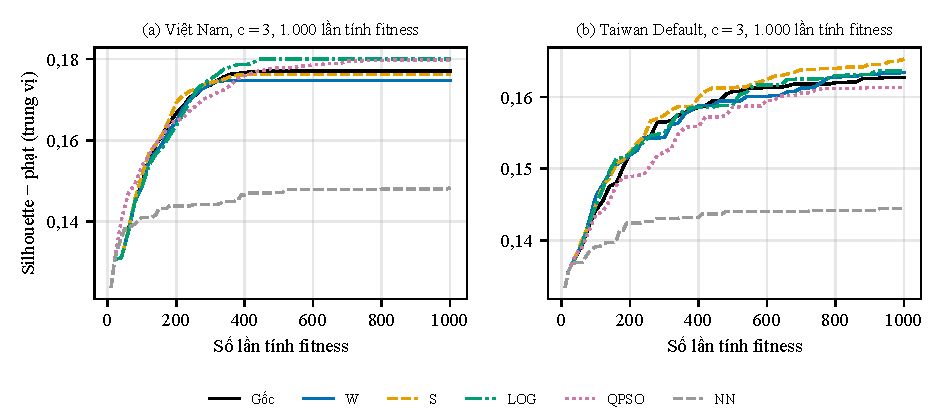
\includegraphics[width=\linewidth]{e9-quy-dao}
\caption{TN4: điểm fitness tốt nhất (Silhouette trừ phạt, trung vị 30 seed) theo số lần tính fitness của 5 phiên bản PSO
và tìm ngẫu nhiên (NN), ngân sách 1.000 lần, $c = 3$}
\label{fig:e9-quy-dao}
\end{figure}

\subsection{Các bản cải tiến không hơn PSO gốc}

Không bản cải tiến nào khác PSO gốc có ý nghĩa ở bất kỳ ô nào, trên cả 3 chỉ số (Bảng~\ref{tab:e9-tong-hop}); trên hình,
quỹ đạo của 5 phiên bản gần như chồng lên nhau. QPSO là bản gần ngưỡng nhất, với trung vị $\Delta r$ cao hơn trên Taiwan Default
$c = 4$ (Bảng~\ref{tab:e9-chenh}) nhưng không còn ý nghĩa sau hiệu chỉnh. Kết quả này ngược với phần tìm tâm, nơi cả 4 bản cải
tiến đều đưa gbest gần cực tiểu hơn PSO gốc (mục~\ref{sec:e5-dat-j}). Một cách giải thích là khác biệt về không gian tìm kiếm:
khi tìm tâm, hộp tìm kiếm rộng bằng miền dữ liệu và PSO gốc ($\omega = 1$) không thu hẹp được quanh gbest; khi tìm trọng số,
hộp chỉ là $[0{,}05;\ 1]^D$ và fitness thay đổi theo bậc, vì nhiều vector trọng số gần nhau cho cùng một phân hoạch cứng, nên
việc thu hẹp bước đi không đem lại thêm bao nhiêu. Nhóm không có phép thử tách riêng nguyên nhân này.

\begin{table}[htbp]
\centering
\caption{TN4 -- Chênh tỉ lệ vỡ nợ của 5 phiên bản PSO khi tìm trọng số thuộc tính}
\label{tab:e9-chenh}
\footnotesize
\setlength{\tabcolsep}{3pt}
\begin{tabular}{@{}lllrrrrrrr@{}}
\toprule
Bộ dữ liệu & c & Ngân sách & FCM & NN & Gốc & W & S & LOG & QPSO \\
\midrule
Việt Nam & 2 & 500 & 0,284 & 0,356 & 0,436\textsuperscript{+} & 0,438\textsuperscript{+} & 0,425\textsuperscript{+} & \textbf{0,447\textsuperscript{+}} & 0,442\textsuperscript{+} \\
 &  & 1.000 &  & 0,363 & 0,447\textsuperscript{+} & 0,438\textsuperscript{+} & 0,446\textsuperscript{+} & 0,441\textsuperscript{+} & \textbf{0,456\textsuperscript{+}} \\
 & 3 & 500 & 0,341 & 0,415 & 0,460\textsuperscript{+} & 0,465\textsuperscript{+} & 0,467\textsuperscript{+} & \textbf{0,468\textsuperscript{+}} & 0,462\textsuperscript{+} \\
 &  & 1.000 &  & 0,415 & 0,473\textsuperscript{+} & 0,471\textsuperscript{+} & \textbf{0,475\textsuperscript{+}} & 0,470\textsuperscript{+} & 0,474\textsuperscript{+} \\
 & 4 & 500 & 0,420 & 0,498 & 0,541\textsuperscript{+} & \textbf{0,557} & 0,544 & 0,536 & 0,552\textsuperscript{+} \\
 &  & 1.000 &  & 0,507 & 0,553\textsuperscript{+} & 0,549\textsuperscript{+} & 0,567\textsuperscript{+} & 0,559\textsuperscript{+} & \textbf{0,572\textsuperscript{+}} \\
\midrule
Taiwan Default & 2 & 500 & 0,036 & 0,009 & 0,031\textsuperscript{+} & \textbf{0,033\textsuperscript{+}} & 0,026\textsuperscript{+} & 0,030\textsuperscript{+} & 0,032\textsuperscript{+} \\
 &  & 1.000 &  & 0,010 & 0,031\textsuperscript{+} & \textbf{0,032\textsuperscript{+}} & 0,031\textsuperscript{+} & \textbf{0,032\textsuperscript{+}} & \textbf{0,032\textsuperscript{+}} \\
 & 3 & 500 & 0,155 & 0,238 & 0,261 & \textbf{0,261} & 0,258 & 0,257 & \textbf{0,261} \\
 &  & 1.000 &  & 0,241 & 0,270\textsuperscript{+} & 0,272\textsuperscript{+} & 0,271\textsuperscript{+} & \textbf{0,274\textsuperscript{+}} & 0,257 \\
 & 4 & 500 & 0,168 & 0,266 & 0,302 & 0,315 & 0,299 & 0,274 & \textbf{0,345\textsuperscript{+}} \\
 &  & 1.000 &  & 0,277 & 0,287 & 0,283 & 0,319 & 0,282 & \textbf{0,358} \\
\bottomrule
\end{tabular}
\par\smallskip\parbox{\linewidth}{\scriptsize Ghi chú: Trung vị 30 seed, m = 2; ngân sách là số lần tính fitness (10 hạt với 500, 20 hạt với 1.000). NN: tìm ngẫu nhiên cùng ngân sách. Đậm: cao nhất trong các phương pháp tìm kiếm cùng ngân sách. \textsuperscript{+} / \textsuperscript{--}: tốt hơn / kém hơn NN có ý nghĩa; \textsuperscript{*} / \textsuperscript{\dag}: tốt hơn / kém hơn PSO gốc có ý nghĩa (Wilcoxon theo cặp seed, Holm toàn họ, $\alpha = 0{,}05$).}
\end{table}


Tăng ngân sách từ 500 lên 1.000 lần tính fitness làm trung vị điểm fitness tốt lên ở 27 trên 30 trường hợp (5 phiên bản,
6 cấu hình), rõ nhất khi có nhiều cụm (trên Taiwan
Default với $c = 4$, PSO gốc từ \soLieuEChinTaiwanKiemChungCBonPsoGocNamKhongKhongDiem{} lên
\soLieuEChinTaiwanKiemChungCBonPsoGocMotKhongKhongKhongDiem), nhưng không đổi kết luận về $\Delta r$ và AUC, trong khi thời gian
gấp đôi (trung vị \soLieuEChinVietNamCBaPsoWNamKhongKhongTTong~s với PSO-W 500 lần trên Việt Nam $c = 3$). Không phát hiện khác
biệt giữa các phiên bản sau hiệu chỉnh Holm; vì họ hiệu chỉnh gộp nhiều phép so nên kiểm định kém nhạy, và kết quả âm này chỉ cho thấy
khác biệt (nếu có) là nhỏ. Về thực hành, PSO gốc hoặc PSO-W với khoảng 500 lần tính fitness là đủ.

% Bình
\section{Kiểm chứng trên mẫu độc lập và giới hạn}
\label{sec:kiem-chung}

Mục này trả lời CH4 và là bước 3 của quy trình đề xuất. Ở TN3, trọng số được tìm và đánh giá trên cùng một mẫu; nếu PSO chỉ
khớp với đặc điểm riêng của mẫu đó, lợi ích sẽ không giữ khi áp trọng số lên khách hàng mới. TN5 học trọng số trên một mẫu
nguồn, rồi trên một mẫu đích độc lập chạy FCM với trọng số đó từ cùng tâm khởi tạo k-means++ như FCM thường. Có 4 chiều
chuyển: 2 mẫu 5.000 khách hàng không giao nhau của Taiwan Default theo cả 2 chiều, và 2 nửa của bộ Việt Nam chia theo
doanh nghiệp theo cả 2 chiều. Mỗi chiều so 5 cách trên mẫu đích: FCM thường, trọng số chuyển từ WFCM giải tích, từ tìm
ngẫu nhiên, từ PSO-W, và PSO-W học ngay trên mẫu đích làm mốc ``tại chỗ'' (Bảng~\ref{tab:e10-ket-qua},
\ref{tab:e10-tong-hop}; \soLieuEMuoiSoLuot{} lượt).

\begin{table}[htbp]
\centering
\caption{TN5 -- trọng số học trên mẫu nguồn, áp lên mẫu đích độc lập}
\label{tab:e10-ket-qua}
\footnotesize
\setlength{\tabcolsep}{2pt}
\begin{tabular}{@{}llrrrrrrrrrr@{}}
\toprule
& & \multicolumn{5}{c}{AUC phân hoạch trên mẫu đích} & \multicolumn{5}{c}{Chênh tỉ lệ vỡ nợ trên mẫu đích} \\
\cmidrule(lr){3-7} \cmidrule(lr){8-12}
Chiều chuyển & c & FCM & WFCM & NN & PSO & Tại chỗ & FCM & WFCM & NN & PSO & Tại chỗ \\
\midrule
Taiwan: thiết kế → kiểm chứng & 2 & \textbf{0,523\textsuperscript{--}} & 0,515 & 0,505\textsuperscript{+} & 0,516 & 0,517 & \textbf{0,036} & 0,024 & 0,008\textsuperscript{+} & 0,030 & 0,033 \\
 & 3 & 0,601\textsuperscript{+} & 0,510\textsuperscript{+} & 0,634 & 0,646 & \textbf{0,664\textsuperscript{--}} & 0,155\textsuperscript{+} & 0,015\textsuperscript{+} & 0,212 & 0,232 & \textbf{0,261\textsuperscript{--}} \\
 & 4 & 0,526\textsuperscript{+} & 0,583 & 0,639 & 0,572 & \textbf{0,645\textsuperscript{--}} & 0,168 & 0,154\textsuperscript{+} & 0,268 & 0,292 & \textbf{0,315} \\
\midrule
Taiwan: kiểm chứng → thiết kế & 2 & 0,509\textsuperscript{+} & 0,500\textsuperscript{+} & 0,521\textsuperscript{+} & \textbf{0,530} & \textbf{0,531} & 0,014\textsuperscript{+} & 0,000\textsuperscript{+} & 0,034\textsuperscript{+} & 0,057 & \textbf{0,059} \\
 & 3 & 0,604\textsuperscript{+} & 0,532\textsuperscript{+} & 0,648 & \textbf{0,653} & 0,650 & 0,160\textsuperscript{+} & 0,048\textsuperscript{+} & 0,226 & \textbf{0,244} & 0,240 \\
 & 4 & 0,525\textsuperscript{+} & 0,617\textsuperscript{+} & 0,644 & \textbf{0,647} & 0,585 & 0,080\textsuperscript{+} & 0,193 & 0,234 & \textbf{0,252} & 0,243 \\
\midrule
Việt Nam: nửa 0 → nửa 1 & 2 & 0,793\textsuperscript{+} & 0,802\textsuperscript{+} & 0,832 & 0,827 & \textbf{0,840} & 0,282\textsuperscript{+} & 0,313\textsuperscript{+} & 0,356\textsuperscript{+} & 0,437 & \textbf{0,442} \\
 & 3 & 0,823 & \textbf{0,835\textsuperscript{--}} & 0,830 & 0,820 & 0,828 & 0,345\textsuperscript{+} & \textbf{0,482} & 0,408\textsuperscript{+} & 0,456 & 0,468 \\
 & 4 & 0,840 & 0,850 & \textbf{0,856} & 0,851 & 0,851 & 0,393\textsuperscript{+} & \textbf{0,613} & 0,489\textsuperscript{+} & 0,517 & 0,588 \\
\midrule
Việt Nam: nửa 1 → nửa 0 & 2 & 0,817\textsuperscript{+} & 0,829\textsuperscript{+} & 0,854\textsuperscript{+} & 0,865 & \textbf{0,870} & 0,295\textsuperscript{+} & 0,311\textsuperscript{+} & 0,362\textsuperscript{+} & 0,417 & \textbf{0,437} \\
 & 3 & 0,855\textsuperscript{+} & \textbf{0,884} & 0,877 & 0,877 & 0,876 & 0,354\textsuperscript{+} & 0,475 & 0,427\textsuperscript{+} & 0,482 & \textbf{0,486} \\
 & 4 & 0,884\textsuperscript{+} & 0,894\textsuperscript{+} & 0,901 & \textbf{0,901} & 0,900 & 0,432\textsuperscript{+} & \textbf{0,622} & 0,518\textsuperscript{+} & 0,584 & 0,548 \\
\bottomrule
\end{tabular}
\par\smallskip\parbox{\linewidth}{\scriptsize Ghi chú: Trung vị 30 seed, m = 2. FCM: trọng số bằng nhau; WFCM, NN, PSO: trọng số học trên mẫu nguồn bằng WFCM giải tích, tìm ngẫu nhiên và PSO-W; Tại chỗ: PSO-W học ngay trên mẫu đích. Mọi cột dùng cùng tâm khởi tạo k-means++ trên mẫu đích. Đậm: cao nhất hàng. Dấu \textsuperscript{+} / \textsuperscript{--} sau một cột: PSO chuyển tốt hơn / kém hơn cột đó có ý nghĩa (Wilcoxon theo cặp seed, Holm toàn họ, $\alpha = 0{,}05$).}
\end{table}


\begin{table}[htbp]
\centering
\caption{TN5 -- số cấu hình trọng số PSO chuyển sang mẫu đích tốt hơn / không khác / kém hơn từng cách khác}
\label{tab:e10-tong-hop}
\footnotesize
\setlength{\tabcolsep}{3pt}
\begin{tabular}{@{}lcccc@{}}
\toprule
PSO chuyển so với & FCM & WFCM chuyển & NN chuyển & PSO tại chỗ \\
\midrule
AUC phân hoạch & 9 / 2 / 1 & 7 / 4 / 1 & 3 / 9 / 0 & 0 / 10 / 2 \\
Chênh tỉ lệ vỡ nợ & 10 / 2 / 0 & 6 / 6 / 0 & 8 / 4 / 0 & 0 / 11 / 1 \\
Silhouette − phạt & 12 / 0 / 0 & 10 / 2 / 0 & 9 / 3 / 0 & 0 / 7 / 5 \\
\bottomrule
\end{tabular}
\par\smallskip\parbox{\linewidth}{\scriptsize Ghi chú: 12 cấu hình (4 chiều chuyển × 3 số cụm), Wilcoxon theo cặp seed, Holm toàn họ, $\alpha = 0{,}05$.}
\end{table}


\subsection{Lợi ích giữ trên mẫu độc lập}

Trọng số PSO học trên mẫu nguồn vẫn làm FCM tách rủi ro tốt hơn FCM thường trên mẫu đích: tốt hơn có ý nghĩa ở
\soLieuEMuoiChenhTiLeFcmKppHon{} trên \soLieuEMuoiSoCauHinh{} cấu hình theo chênh tỉ lệ vỡ nợ (không cấu hình nào kém hơn) và
\soLieuEMuoiAucCungFcmKppHon{} cấu hình theo AUC phân hoạch. Trên Việt Nam (nửa 0 sang nửa 1, $c = 2$), $\Delta r$ tăng từ
\soLieuEMuoiVnKhongMotCHaiFcmKppChenhTiLe{} lên \soLieuEMuoiVnKhongMotCHaiPsoChuyenChenhTiLe; trên Taiwan Default (mẫu kiểm
chứng sang mẫu thiết kế, $c = 4$), AUC tăng từ \soLieuEMuoiTaiwanKcTkCBonFcmKppAucCung{} lên
\soLieuEMuoiTaiwanKcTkCBonPsoChuyenAucCung. Cấu hình duy nhất kém hơn FCM thường (theo AUC, không theo $\Delta r$) là Taiwan
Default với $c = 2$ (mẫu thiết kế sang mẫu kiểm chứng), đúng chỗ PSO đã yếu ở TN3.

So với PSO học ngay trên mẫu đích, trọng số chuyển sang không khác có ý nghĩa ở \soLieuEMuoiChenhTiLePsoTaiChoBang{} cấu hình
theo $\Delta r$ và \soLieuEMuoiAucCungPsoTaiChoBang{} cấu hình theo AUC. Phần mất đi tập trung ở một chiều chuyển của Taiwan
Default (mẫu thiết kế sang mẫu kiểm chứng) với $c = 3, 4$; chẳng hạn với $c = 4$, AUC là
\soLieuEMuoiTaiwanTkKcCBonPsoChuyenAucCung{} so với \soLieuEMuoiTaiwanTkKcCBonPsoTaiChoAucCung{} khi học tại chỗ, vẫn cao hơn FCM
thường. Trọng số học ở 2 mẫu cũng giống nhau: cosine trung vị giữa trọng số học trên mẫu nguồn và trên mẫu đích là
\soLieuEMuoiTaiwanTkKcCosTrongSo{} ở Taiwan Default và \soLieuEMuoiVnKhongMotCosTrongSo{} ở Việt Nam. Tuy vậy, do mọi trọng số đều dương,
hai vector ngẫu nhiên trong miền tìm kiếm cũng có cosine khoảng 0,8, nên con số này chưa cho thấy từng giá trị trọng số ổn
định giữa 2 mẫu; thứ giữ được là lợi ích của phân hoạch.

Phần lợi ích do cơ chế bầy đàn cũng giữ: trọng số PSO chuyển sang tốt hơn trọng số tìm ngẫu nhiên chuyển sang ở
\soLieuEMuoiChenhTiLeNgauNhienChuyenHon{} cấu hình theo $\Delta r$ (không cấu hình nào kém hơn), rõ nhất trên Việt Nam ở mọi
chiều và mọi $c$. So với WFCM giải tích chuyển sang, PSO tốt hơn ở \soLieuEMuoiChenhTiLeWfcmChuyenHon{} cấu hình theo $\Delta r$
và \soLieuEMuoiAucCungWfcmChuyenHon{} cấu hình theo AUC; trên Taiwan Default công thức lại gần như xoá khả năng tách rủi ro
($\Delta r$ \soLieuEMuoiTaiwanTkKcCBaWfcmChuyenChenhTiLe{} với $c = 3$), giống TN3.

\subsection{Khi nào PSO tìm trọng số không có ích}
\label{sec:khong-co-ich}

Trên 7 bộ của TN3, PSO kém FCM thường có ý nghĩa ở \soLieuETamAucCungFcmKppKem{} cấu hình theo AUC, đều với
$c = 2$ (Australian, Polish, South German, Taiwan Bankruptcy, Taiwan Default). Với 2 cụm, FCM thường đã tách theo trục có
liên quan tới vỡ nợ, còn PSO tìm một cách tách đẹp hơn về hình học (Silhouette cao hơn) nhưng ít liên quan tới rủi ro hơn:
fitness không nhìn nhãn nên không có gì bảo đảm 2 mục tiêu trùng nhau. Ở Australian, South German và Taiwan Bankruptcy với
$c \ge 3$ (và Polish với $c = 4$), FCM thường cho nghiệm gần sụp, cụm nhỏ nhất chỉ chiếm \soLieuETamSouthGermanCBaFcmKppCumNhoNhat{} dữ liệu (South
German, $c = 3$) hoặc \soLieuETamAustralianCBonFcmKppCumNhoNhat{} (Australian, $c = 4$). Phạt cụm nhỏ buộc PSO tìm phân hoạch
cân hơn; trên South German điều này làm AUC tăng (\soLieuETamSouthGermanCBonFcmKppAucCung{} lên
\soLieuETamSouthGermanCBonPsoTrongSoAucCung{} với $c = 4$), nhưng trên Australian và Polish thì không tăng có ý nghĩa. Trên
Taiwan Bankruptcy với $c = 4$, PSO giảm số cụm rỗng nhưng cụm nhỏ nhất vẫn dưới 0,1\% dữ liệu ở trung vị, tức phạt cụm nhỏ
không đạt được.

Tổng hợp TN3 và TN5, PSO tìm trọng số có ích khi dữ liệu có nhiều thuộc tính số liên tục đo các khía cạnh khác nhau của
rủi ro, như các tỉ số tài chính của bộ Việt Nam hay lịch sử trả nợ và dư nợ của bộ Taiwan Default: ở đó PSO có ích với mọi
$c$ đã thử trên Việt Nam và với $c = 3, 4$ trên Taiwan Default, còn $c = 2$ là chỗ yếu nhất. Trên các bộ mà đa số thuộc tính là mã thứ bậc hoặc định danh (South German,
German, Australian) hoặc có đuôi cực dài (2 bộ phá sản), FCM thường đã gần sụp và trọng số không cứu được. Vì fitness không
nhìn nhãn, bước 3 của quy trình đề xuất (mục~\ref{sec:de-xuat}) là cần thiết: dùng nhãn lịch sử trên một mẫu độc lập để quyết
định có áp trọng số hay không, đúng như TN5 làm.


\section{Diễn giải các phân khúc rủi ro}
\label{sec:dien-giai}

Mục này đọc các phân khúc với $c = 3$, $m = 2$, seed 1000, đặt phân hoạch FCM thường cạnh phân hoạch FCM có trọng số do
PSO-W tìm (TN3) trên cùng tâm khởi tạo (Bảng~\ref{tab:e4-profile-viet_nam}, \ref{tab:e4-profile-taiwan_kiem_chung}). Cụm được
đánh số theo tỉ lệ vỡ nợ tăng dần; cột ``mơ hồ'' là tỉ lệ khách hàng có độ thuộc lớn nhất dưới 0,6; 5 thuộc tính in ra (thang
gốc) là 5 thuộc tính có khoảng trung bình giữa các cụm của phân hoạch có trọng số rộng nhất, tính theo độ lệch chuẩn.

\begin{table}[htbp]
\centering
\caption{Profile cụm FCM thường và FCM có trọng số do PSO tìm trên Việt Nam (c = 3, seed 1000): trung bình giá trị gốc}
\label{tab:e4-profile-viet_nam}
\footnotesize
\setlength{\tabcolsep}{3pt}
\begin{tabular}{@{}lrrrrrrrrr@{}}
\toprule
Phương pháp & Cụm & Cỡ (\%) & Vỡ nợ (\%) & Mơ hồ (\%) & \rotatebox{60}{X17} & \rotatebox{60}{X11} & \rotatebox{60}{X6} & \rotatebox{60}{X10} & \rotatebox{60}{X8} \\
\midrule
FCM (k-means++) &1 & 40,9 & 1,3 & 100,0 & 2,09 & 0,19 & 0,24 & 0,26 & 0,22 \\
 &2 & 24,8 & 2,5 & 100,0 & 0,47 & 0,36 & 0,24 & 0,58 & 0,54 \\
 &3 & 34,3 & 35,4 & 90,7 & 0,39 & 0,67 & 1,28 & 2,54 & 2,13 \\
\midrule
PSO trọng số &1 & 56,6 & 3,1 & 17,6 & 0,51 & 0,34 & 0,29 & 0,65 & 0,60 \\
 &2 & 23,7 & 7,6 & 20,4 & 3,26 & 0,23 & 0,29 & 0,42 & 0,32 \\
 &3 & 19,6 & 49,8 & 26,7 & 0,24 & 0,73 & 1,86 & 3,34 & 2,74 \\
\bottomrule
\end{tabular}
\par\smallskip\parbox{\linewidth}{\scriptsize Ghi chú: cụm đánh số theo tỉ lệ vỡ nợ tăng dần; mơ hồ: tỉ lệ điểm trong cụm có độ thuộc lớn nhất $<$ 0,6; thuộc tính chọn là 5 thuộc tính có khoảng trung bình giữa các cụm (PSO trọng số) rộng nhất tính theo độ lệch chuẩn. X17: P/S; X11: phải trả người bán/tổng tài sản; X6: tổng nợ/VCSH; X10: phải trả người bán/VCSH; X8: nợ ngắn hạn/VCSH.}
\end{table}


Trên Việt Nam, trọng số làm phân khúc rủi ro cao gọn và rõ hơn. Với FCM thường, cụm rủi ro cao chiếm
\soLieuEBonVietNamFcmKppCumBaCo\% doanh nghiệp với tỉ lệ khó khăn tài chính \soLieuEBonVietNamFcmKppCumBaVoNo\%; với trọng số do PSO tìm,
cụm này chỉ còn \soLieuEBonVietNamPsoTrongSoCumBaCo\% doanh nghiệp nhưng tỉ lệ khó khăn tài chính lên \soLieuEBonVietNamPsoTrongSoCumBaVoNo\%,
còn cụm rủi ro thấp chiếm \soLieuEBonVietNamPsoTrongSoCumMotCo\% với tỉ lệ \soLieuEBonVietNamPsoTrongSoCumMotVoNo\%. Cụm rủi ro
cao có các tỉ số nợ trên vốn chủ sở hữu (X6, X8, X10) cao nhất, đúng các thuộc tính PSO đánh trọng số cao ở
Hình~\ref{fig:e8-trong-so}; tỉ số phải trả người bán trên tổng tài sản (X11) cũng cao dù trọng số của nó thấp. Cụm giữa được tách theo định giá: P/S (X17) cao gấp nhiều lần 2 cụm
còn lại, tức nhóm doanh nghiệp được thị trường định giá cao so với doanh thu, có tỉ lệ khó khăn tài chính \soLieuEBonVietNamPsoTrongSoCumHaiVoNo\%,
dưới mức chung của bộ dữ liệu. Độ thuộc cũng có ý nghĩa trở lại: tỉ lệ khách hàng mơ hồ giảm từ \soLieuEBonVietNamFcmKppCumBaMoHo--\soLieuEBonVietNamFcmKppCumMotMoHo\% ở FCM thường
xuống \soLieuEBonVietNamPsoTrongSoCumMotMoHo--\soLieuEBonVietNamPsoTrongSoCumBaMoHo\%, nên độ thuộc phân biệt được doanh nghiệp
điển hình với doanh nghiệp ``biên'', đúng lý do chọn phân cụm mờ ở Chương~\ref{chap:tong-quan}.

\begin{table}[htbp]
\centering
\caption{Profile cụm FCM thường và FCM có trọng số do PSO tìm trên Taiwan Default (c = 3, seed 1000): trung bình giá trị gốc}
\label{tab:e4-profile-taiwan_kiem_chung}
\footnotesize
\setlength{\tabcolsep}{3pt}
\begin{tabular}{@{}lrrrrrrrrr@{}}
\toprule
Phương pháp & Cụm & Cỡ (\%) & Vỡ nợ (\%) & Mơ hồ (\%) & \rotatebox{60}{PAY\_3} & \rotatebox{60}{PAY\_5} & \rotatebox{60}{PAY\_2} & \rotatebox{60}{PAY\_4} & \rotatebox{60}{PAY\_6} \\
\midrule
FCM (k-means++) &1 & 44,3 & 15,9 & 100,0 & −0,01 & −0,04 & −0,02 & −0,03 & −0,03 \\
 &2 & 25,1 & 21,7 & 75,1 & −1,16 & −1,36 & −1,06 & −1,30 & −1,44 \\
 &3 & 30,6 & 31,4 & 100,0 & 0,42 & 0,33 & 0,44 & 0,37 & 0,29 \\
\midrule
PSO trọng số &1 & 46,8 & 13,2 & 100,0 & −0,10 & −0,11 & −0,16 & −0,09 & −0,07 \\
 &2 & 27,0 & 20,4 & 86,2 & −1,25 & −1,36 & −1,13 & −1,32 & −1,40 \\
 &3 & 26,2 & 39,8 & 100,0 & 0,82 & 0,62 & 0,91 & 0,65 & 0,46 \\
\bottomrule
\end{tabular}
\par\smallskip\parbox{\linewidth}{\scriptsize Ghi chú: cụm đánh số theo tỉ lệ vỡ nợ tăng dần; mơ hồ: tỉ lệ điểm trong cụm có độ thuộc lớn nhất $<$ 0,6; thuộc tính chọn là 5 thuộc tính có khoảng trung bình giữa các cụm (PSO trọng số) rộng nhất tính theo độ lệch chuẩn. PAY\_k: tình trạng trả nợ ở tháng thứ k trước tháng quan sát (theo mô tả của UCI: $-1$ trả đúng hạn, $1$ đến $9$ trễ hạn 1 đến 9 tháng; dữ liệu còn các mã $-2$ và $0$ không được giải thích); giá trị dương là có trễ hạn.}
\end{table}


Trên Taiwan Default, trục phân khúc ở cả 2 phân hoạch là lịch sử trả nợ: 5 thuộc tính khác nhau nhiều nhất giữa các cụm đều
là tình trạng trả nợ các tháng (PAY\_2--PAY\_6), và cụm rủi ro cao gồm khách hàng có giá trị PAY dương, tức có trễ hạn. Trọng số
làm trục này rõ hơn: cụm rủi ro cao có PAY trung bình cao hơn và tỉ lệ vỡ nợ \soLieuEBonTaiwanKiemChungPsoTrongSoCumBaVoNo\%
(so với \soLieuEBonTaiwanKiemChungFcmKppCumBaVoNo\% ở FCM thường), còn cụm rủi ro thấp có tỉ lệ
\soLieuEBonTaiwanKiemChungPsoTrongSoCumMotVoNo\% (so với \soLieuEBonTaiwanKiemChungFcmKppCumMotVoNo\%). Khác với Việt Nam, độ
thuộc vẫn chia gần đều: tỉ lệ khách hàng mơ hồ ở 2 cụm vẫn là \soLieuEBonTaiwanKiemChungPsoTrongSoCumBaMoHo\%. Với $m = 2$, trọng
số làm phân hoạch cứng tách rủi ro tốt hơn nhưng chưa làm các tâm tách đủ xa để độ thuộc có ý nghĩa trên bộ này; chọn $m$ nhỏ
hơn (mục~\ref{sec:vi-sao}) là hướng bổ sung.

% Bình
\section{Đánh giá chung các thuật toán}
\label{sec:danh-gia-chung}

Các mục trên trả lời từng câu hỏi nghiên cứu. Mục này nhìn lại theo từng thuật toán: mỗi phiên bản PSO đã được dùng ở 2
vai trò, cùng với FCM, WFCM giải tích và tìm ngẫu nhiên làm đối chứng (Bảng~\ref{tab:ch3-danh-gia}).

\begin{table}[htbp]
\centering
\caption{Đánh giá các thuật toán trên dữ liệu tín dụng theo 2 vai trò}
\label{tab:ch3-danh-gia}
\footnotesize
\setlength{\tabcolsep}{3pt}
\renewcommand{\arraystretch}{1.15}
\begin{tabular}{@{}>{\raggedright\arraybackslash}p{2.3cm}>{\raggedright\arraybackslash}p{5.4cm}>{\raggedright\arraybackslash}p{5.0cm}>{\raggedright\arraybackslash}p{2.1cm}@{}}
\toprule
Thuật toán & Khi tìm tâm khởi tạo (TN1, TN2) & Khi tìm trọng số (TN3, TN4) & Thời gian \\
\midrule
FCM k-means++ & Đạt $J_m$ tốt nhất ở mọi lượt trên 2 bộ chính; chỉ kém PSO 2--3/30 seed ở một cấu hình nhiều cực tiểu & Mốc không trọng số; thua PSO
trên Việt Nam (mọi $c$) và Taiwan Default ($c = 3, 4$) & \soLieuETamThoiGianFcm~s \\
\addlinespace
WFCM giải tích & --- & Ngang hoặc hơn PSO trên Việt Nam $c = 3, 4$; gần như mất khả năng tách rủi ro trên Taiwan Default & cỡ một
lần FCM \\
\addlinespace
Tìm ngẫu nhiên & --- & Thua PSO về fitness ở \soLieuETamSilhouetteNgauNhienTrongSoHon/\soLieuETamSoCauHinh{} cấu hình; ngừng cải
thiện sớm & cùng ngân sách \\
\addlinespace
PSO gốc & gbest xa cực tiểu nhất (22--26\% trên Taiwan Default); không cải thiện khi tăng số vòng & Không khác các bản cải tiến
ở ô nào & 25--27~s (500 lần tính fitness) \\
PSO-W & Cùng QPSO gần cực tiểu nhất (9,5\% với 30 hạt, 50 vòng) & Dùng ở TN3; không khác PSO gốc & như PSO gốc \\
PSO-S & Kém nhất trong 4 bản cải tiến & Không khác PSO gốc & như PSO gốc \\
PSO-LOG & Giữa PSO-W và PSO-S & Không khác PSO gốc & như PSO gốc \\
QPSO & Tốt nhất trên Việt Nam và Taiwan chưa log & Gần ngưỡng nhất ($\Delta r$, Taiwan $c = 4$), không có ý nghĩa sau Holm &
như PSO gốc \\
\bottomrule
\end{tabular}
\par\smallskip\parbox{\linewidth}{\scriptsize Ở vai trò tìm tâm, sau khi FCM chạy, mọi phiên bản cho cùng nghiệm với FCM
k-means++ và chậm hơn khoảng \soLieuENamTaiwanKiemChungCBaTiLeThoiGianTv{} lần trên Taiwan Default; thời gian ở cột cuối là của
vai trò tìm trọng số (trung vị).}
\end{table}

Ba nhận xét rút ra từ bảng. Thứ nhất, \emph{các phiên bản PSO có thứ hạng rõ khi được đo như thuật toán tối ưu}: 4 bản cải
tiến đưa gbest gần cực tiểu hơn PSO gốc, PSO-W và QPSO tốt nhất, đúng như lý do chúng được đề xuất trong tài
liệu~\cite{shi1998inertia,qian2022psofcm,zhang2025qpsofcm}. Thứ hai, \emph{thứ hạng đó không chuyển thành kết quả phân cụm}: khi
tìm tâm, FCM chạy sau đưa mọi điểm xuất phát về cùng một cực tiểu; khi tìm trọng số, fitness thay đổi theo bậc và hộp tìm kiếm
hẹp, nên PSO gốc đã đủ. Thứ ba, \emph{vai trò của PSO quyết định kết quả, còn phiên bản thì không}: cùng 5 thuật toán, ở vai
trò tìm tâm không đem lại gì so với FCM k-means++, ở vai trò tìm trọng số làm phân khúc tách rủi ro tốt hơn trên 2 bộ chính
và tối ưu fitness tốt hơn tìm ngẫu nhiên. Với dữ liệu tín dụng như của nhóm, khi cần độ thuộc để nhận ra khách hàng
``biên'', lựa chọn hợp lý là FCM khởi tạo k-means++, cộng PSO gốc hoặc PSO-W tìm trọng số với khoảng 500 lần tính fitness,
và giữ WFCM giải tích làm phương án rẻ để so; khi chỉ cần phân hoạch cứng với 3 cụm trở lên, K-means không trọng số tách rủi
ro tốt hơn trên 2 bộ chính và nên được so trước.

\section*{Tiểu kết Chương 3}
\addcontentsline{toc}{section}{Tiểu kết Chương 3}
\label{sec:tong-ket}

Bảng~\ref{tab:ch3-tong-ket} tóm tắt câu trả lời cho 4 câu hỏi nghiên cứu; số liệu đã trình bày ở các mục trên.

\begin{table}[htbp]
\centering
\caption{Tổng kết kết quả thực nghiệm}
\label{tab:ch3-tong-ket}
\footnotesize
\setlength{\tabcolsep}{3pt}
\begin{tabular}{@{}>{\raggedright\arraybackslash}p{3.4cm}>{\raggedright\arraybackslash}p{11.0cm}@{}}
\toprule
Câu hỏi & Kết quả \\
\midrule
CH1: PSO tìm tâm (hướng ban đầu) & Không giúp FCM. $J_m$ hầu như chỉ có 1 cực tiểu
(\soLieuESauSoCauHinhMotCucTieu/\soLieuESauSoCauHinh{} cấu hình) hoặc FCM sụp; mọi tổ hợp PSO cho cùng nghiệm với FCM k-means++
trên 2 bộ chính; ở các cấu hình nhiều cực tiểu chỉ hơn k-means++ nhiều nhất 2--3/30 seed, trong khi chậm hơn nhiều lần. \\
CH2: PSO tìm trọng số & Có ích rõ trên 2 bộ chính: tốt hơn FCM thường có ý nghĩa ở mọi $c$ trên Việt Nam và $c = 3, 4$ trên
Taiwan Default (Việt Nam $c = 2$: $\Delta r$ \soLieuETamVietNamCHaiFcmKppChenhTiLe{} lên
\soLieuETamVietNamCHaiPsoTrongSoChenhTiLe). Hơn tìm ngẫu nhiên cùng ngân sách về fitness ở
\soLieuETamSilhouetteNgauNhienTrongSoHon/\soLieuETamSoCauHinh{} cấu hình. WFCM giải tích ngang hoặc hơn PSO trên Việt Nam $c = 3, 4$ nhưng
hỏng trên Taiwan Default. K-means không trọng số tách rủi ro tốt hơn PSO với $c = 3, 4$ trên Việt Nam và $c = 4$ trên Taiwan
Default (theo $\Delta r$), kém PSO với $c = 2$. Trọng số có nghĩa kinh tế. \\
CH3: 5 phiên bản & Mọi phiên bản hơn tìm ngẫu nhiên (fitness \soLieuEChinGocNgauNhienDiemHon--12/\soLieuEChinSoO{} ô,
$\Delta r$ 8--9/\soLieuEChinSoO{} ô); không phát hiện bản cải tiến nào khác PSO gốc sau hiệu chỉnh Holm. Tăng ngân sách từ 500 lên 1.000 lần tính
fitness chỉ cải thiện ít. \\
CH4: kiểm chứng và giới hạn & Trọng số học trên mẫu nguồn vẫn tốt hơn FCM thường trên mẫu đích độc lập
(\soLieuEMuoiChenhTiLeFcmKppHon/\soLieuEMuoiSoCauHinh{} cấu hình theo $\Delta r$) và không khác học tại chỗ ở
\soLieuEMuoiChenhTiLePsoTaiChoBang/\soLieuEMuoiSoCauHinh. Không có ích trên các bộ FCM gần sụp và với $c = 2$ (cả Taiwan Default theo AUC). \\
\bottomrule
\end{tabular}
\end{table}

Thực nghiệm gồm 2 giai đoạn. Ở hướng ban đầu, PSO tìm tâm làm giảm cùng hàm $J_m$ với FCM, và vì hàm này trên dữ liệu
tín dụng đã thử hầu như chỉ có 1 cực tiểu, PSO không đem lại gì dù các bản cải tiến tối ưu tốt hơn PSO gốc, đúng như các so sánh độc lập trong tài liệu. Sau khi chuyển hướng, PSO tìm trọng
số thuộc tính (thứ FCM không tự tối ưu được) và làm các phân khúc tách rủi ro tốt hơn rõ trên 2 bộ chính, lợi ích giữ trên
mẫu độc lập, và phần lợi ích do cơ chế bầy đàn, đo bằng đối chứng tìm ngẫu nhiên, thấy rõ trên Việt Nam. Ở vai trò này, không
phát hiện khác biệt giữa các phiên bản PSO. Lợi ích không phổ quát: fitness không dùng nhãn nên cần kiểm phân hoạch bằng nhãn lịch sử, đúng bước 3 của quy trình
đề xuất. Hai giới hạn cần đọc kèm: chỉ có 2 bộ dữ liệu chính, và mọi kết quả trọng số dùng $m = 2$ với một fitness.

% ============================================================
% 04-ket-luan.tex — Kết luận và hướng phát triển (Bình)
% Số liệu dùng macro \soLieu... (results/so-lieu*.tex). Bốn câu hỏi CH1–CH4 khớp Mở đầu và Tiểu kết Chương 1.
% ============================================================
\chapter*{KẾT LUẬN VÀ HƯỚNG PHÁT TRIỂN}
\addcontentsline{toc}{chapter}{KẾT LUẬN VÀ HƯỚNG PHÁT TRIỂN}

\section*{Kết quả đạt được}

Tiểu luận đi theo 2 giai đoạn. Nhóm bắt đầu bằng cách ghép phổ biến, dùng PSO tìm tâm khởi tạo cho FCM, và thấy cách này
không cải thiện FCM trên dữ liệu tín dụng, đúng như các so sánh độc lập trong tài liệu. Nhóm chuyển sang dùng PSO tìm trọng số
thuộc tính cho FCM, đề xuất 3 lựa chọn thiết kế cho bài toán này, so 5 phiên bản PSO và kiểm trọng số trên mẫu độc lập.
Câu trả lời cho 4 câu hỏi nghiên cứu, với số liệu ở Bảng~\ref{tab:ch3-tong-ket}, như sau.

\emph{CH1 (hướng ban đầu).} PSO tìm tâm khởi tạo không giúp FCM: các bản cải tiến tối ưu tốt hơn PSO gốc, nhưng sau khi FCM
chạy, mọi phiên bản cho cùng nghiệm với FCM khởi tạo k-means++ mà chậm hơn (khoảng 1,7 lần trên Việt Nam, 24 lần trên Taiwan Default). Nguyên nhân là hàm mục tiêu trên dữ liệu
đã thử hầu như chỉ có 1 cực tiểu, nên PSO và FCM làm giảm cùng một hàm. Các bài báo PSO--FCM báo kết quả tốt hơn chủ yếu vì
so với FCM khởi tạo ngẫu nhiên và không cùng ngân sách.

\emph{CH2 (đề xuất).} PSO tìm trọng số làm các phân khúc tách rủi ro tốt hơn FCM thường có ý nghĩa trên 2 bộ chính (Việt Nam
ở mọi số cụm, Taiwan Default với 3 và 4 cụm); với 2 cụm trên Việt Nam, chênh tỉ lệ vỡ nợ giữa các cụm tăng từ
\soLieuETamVietNamCHaiFcmKppChenhTiLe{} lên \soLieuETamVietNamCHaiPsoTrongSoChenhTiLe. So với tìm ngẫu nhiên cùng ngân sách, PSO
tối ưu fitness tốt hơn ở đa số cấu hình, nhưng chỉ tách rủi ro tốt hơn ở vài cấu hình, chủ yếu trên Việt Nam; trọng số tính bằng công thức không thay được PSO trên Taiwan Default.
Lợi ích này đo so với FCM $m = 2$: với ba, 4 cụm, K-means không trọng số vẫn tách rủi ro tốt hơn trên Việt Nam (và theo
chênh tỉ lệ vỡ nợ trên Taiwan Default với 4 cụm), nên FCM có trọng số chỉ đáng dùng khi cần độ thuộc. Trọng số tìm
được có nghĩa kinh tế: lịch sử trả nợ trên Taiwan Default, định giá và đòn bẩy trên Việt Nam.

\emph{CH3 (so sánh các phiên bản).} Cả 5 phiên bản đều hơn tìm ngẫu nhiên cùng ngân sách, nhưng không bản cải tiến nào hơn
PSO gốc, ngược với vai trò tìm tâm. Trong vai trò tìm trọng số, không phát hiện khác biệt giữa các phiên bản sau hiệu chỉnh Holm, nên
chọn phiên bản nào không phải yếu tố quyết định.

\emph{CH4 (kiểm chứng và giới hạn).} Trọng số học trên một mẫu vẫn cải thiện phân khúc trên mẫu kia so với FCM thường; theo chênh tỉ lệ
vỡ nợ, kết quả không khác học ngay trên mẫu đó ở \soLieuEMuoiChenhTiLePsoTaiChoBang{} trên \soLieuEMuoiSoCauHinh{} cấu hình, còn theo AUC
kém hơn ở \soLieuEMuoiAucCungPsoTaiChoKem{} cấu hình. Lợi ích không phổ quát: trên các bộ mà FCM thường đã gần sụp và với 2 cụm (kể cả Taiwan Default, mức chênh
nhỏ), PSO không có ích hoặc kém hơn, vì fitness không dùng nhãn.

Về thực hành, khi phân khúc khách hàng tín dụng bằng FCM, không nên dùng PSO tìm tâm: khởi tạo k-means++ là đủ, và nên chẩn
đoán số cực tiểu trước khi nghĩ tới PSO cho tâm. Nên dùng PSO để tìm trọng số thuộc tính theo đề xuất, và chỉ áp trọng số
khi nó cải thiện phân khúc trên một mẫu có nhãn lịch sử không dùng để tìm trọng số (mục~\ref{sec:de-xuat}).

\section*{Hạn chế}

\begin{itemize}
  \item Phần trọng số dùng một fitness (Silhouette trên không gian gốc, phạt cụm dưới 5\%), một số mũ $m = 2$ và $c$ từ 2 đến
  4; với $m = 2$ trên Taiwan Default, độ thuộc vẫn chia gần đều ngay cả khi phân hoạch cứng đã tách rủi ro tốt hơn.
  \item Hai chỉ số chính dùng nhãn để đánh giá và tính trên chính mẫu được phân cụm; TN5 kiểm trên mẫu độc lập nhưng chỉ cho
  2 bộ chính. Bộ Việt Nam gồm các quan sát doanh nghiệp--năm không độc lập; 2 nửa được chia theo doanh nghiệp để giảm ảnh
  hưởng này.
  \item Đối chứng chính là FCM với $m = 2$, vốn gần suy biến khi có từ 3 cụm; K-means không trọng số được thêm làm mốc tham
  chiếu và tách rủi ro tốt hơn ở các cấu hình này. Chưa thử PSO tìm trọng số cho K-means hay cho FCM với $m$ nhỏ hơn.
  \item Kiểm định lấy seed làm đơn vị, nên chỉ đo dao động của thuật toán trên mẫu đã cho, không đo dao động do lấy mẫu khách
  hàng. Nhãn của bộ Việt Nam được định nghĩa từ chính các đại lượng tài chính có trong thuộc tính (vốn chủ sở hữu, EBITDA, lãi
  vay) và gán theo doanh nghiệp, nên mức tách rủi ro trên bộ này có thể cao hơn khi dự báo thật.
  \item Chỉ có 2 bộ dữ liệu chính, trong đó bộ Việt Nam và cả 2 mẫu Taiwan Default đã được dùng ở các thí nghiệm thử; 5 bộ phụ cho thấy kết quả không khái quát
  được cho mọi dữ liệu tín dụng.
  \item Silhouette của fitness tính trên mẫu 1.000 điểm nên có nhiễu mẫu; ngân sách 500 và 1.000 lần tính fitness nhỏ so với
  các bài đã đọc, và các phiên bản dùng chung tham số thay vì tham số riêng của từng bài.
  \item Phần tìm tâm dùng $m = 2$, $c = 3$ trong thí nghiệm chính, một chế độ gần suy biến; kiểm lại với $m = 1{,}5$ cho cùng
  kết luận nhưng chỉ trên 2 bộ dữ liệu. ``Số cực tiểu'' là số mức $J_m$ quan sát được, không phải số cực tiểu thật.
  \item Thời gian được đo khi nhiều tiến trình chạy song song và máy còn chạy việc khác, nên chỉ chênh lệch nhiều lần là đáng
  tin.
  \item Danh sách thuộc tính gần trùng của bộ Việt Nam được chọn thủ công và bỏ sót X10 (tương quan 0,966 với X8).
\end{itemize}

\section*{Hướng phát triển}

Ba hướng tiếp nối trực tiếp phần trọng số: tìm trọng số cùng lúc với $m$ và $c$ thay vì cố định chúng, thử các fitness khác
Silhouette (chẳng hạn chỉ số mờ như XB khi các tâm tách rõ), và cho phép trọng số riêng cho từng cụm như WFCM của bài
06~\cite{liu2021msgwo}. Hai hướng khác là xử lý dữ liệu hỗn hợp số và định danh để FCM không sụp trên các bộ tín dụng cá nhân,
và dùng các phân khúc có trọng số làm đầu vào cho mô hình chấm điểm theo cụm như Bosker và cộng sự~\cite{bosker2025clustered}.


% ============================================================
% TÀI LIỆU THAM KHẢO
% ============================================================


\newpage
\begingroup\sloppy\emergencystretch=3em
\printbibliography[title={TÀI LIỆU THAM KHẢO}]
\addcontentsline{toc}{chapter}{TÀI LIỆU THAM KHẢO}
\endgroup

% ============================================================
% PHỤ LỤC
% ============================================================

\appendix
\addtocontents{toc}{\protect\renewcommand{\protect\chaptertocprefix}{PHỤ LỤC}}
% ============================================================
% phu-luc-b-ma-nguon.tex — Phụ lục mã nguồn: mã nguồn, lệnh chạy lại, phân công đọc hiểu code, (Giang)
% ============================================================
\chapter{MÃ NGUỒN VÀ DỮ LIỆU}
\label{app:code}

\section*{Cấu trúc thư mục}

Mã nguồn viết bằng Python 3.9 với NumPy, SciPy, pandas và scikit-learn (phiên bản ghim trong
\texttt{requirements.txt}). FCM và các phiên bản PSO được cài bằng NumPy. scikit-learn chỉ dùng cho Silhouette và AUC, còn
scikit-fuzzy chỉ dùng trong phép thử để đối chiếu FCM. Bảng~\ref{tab:pl-ma-nguon} liệt kê các tệp dùng cho kết quả trong
bài. Thư mục \texttt{code/} còn chứa các phương pháp của phiên bản trước (thuật toán GWO, các cách ghép khác), không trình bày ở đây.

{\footnotesize
\begin{longtable}{@{}>{\raggedright\arraybackslash}p{4.4cm}>{\raggedright\arraybackslash}p{10.4cm}@{}}
\caption{Các tệp mã nguồn dùng trong bài}\label{tab:pl-ma-nguon}\\
\toprule
\textbf{Tệp} & \textbf{Nội dung} \\
\midrule
\endfirsthead
\toprule
\textbf{Tệp} & \textbf{Nội dung} \\
\midrule
\endhead
\texttt{fcm.py} & FCM (mục~\ref{sec:fcm}), khởi tạo U ngẫu nhiên hoặc k-means++ \\
\texttt{pso\_co\_so.py} & PSO có vận tốc dùng chung cho PSO gốc, PSO-W, PSO-S, PSO-LOG (mục~\ref{sec:pso-goc}) \\
\texttt{thuat\_toan\_a.py}, \texttt{thuat\_toan\_b.py} & Lịch quán tính S và LOG (mục~\ref{sec:pso-s-log}); QPSO (mục~\ref{sec:qpso}) \\
\texttt{cach\_ket\_hop.py} & Bài toán trọng số (fitness Silhouette trên không gian gốc, phạt cụm nhỏ), phân hoạch theo trọng số, WFCM giải tích (mục~\ref{sec:wfcm}, \ref{sec:pso-trong-so-pp}) \\
\texttt{pso\_trong\_so.py} & PSO tìm trọng số thuộc tính với 5 phiên bản, tìm ngẫu nhiên cùng ngân sách (mục~\ref{sec:pso-trong-so-pp}) \\
\texttt{pso\_khoi\_tao.py} & PSO tìm tâm khởi tạo cho FCM, 5 phiên bản, đối chứng điểm ngẫu nhiên (mục~\ref{sec:pso-khoi-tao}) \\
\texttt{giao\_dien.py} & Giao diện chung \texttt{fit(X, c, m, rng, max\_fe)}, FCM k-means++, FCM tinh chỉnh từ bộ tâm \\
\texttt{chi\_so\_danh\_gia.py}, \texttt{danh\_gia.py} & PC, PE, XB, Silhouette, AUC, chênh tỉ lệ vỡ nợ, đánh giá một lượt \\
\texttt{tien\_xu\_ly.py}, \texttt{mo\_ta\_du\_lieu.py} & Nạp, tiền xử lý dữ liệu (mục~\ref{sec:tien-xu-ly}), 2 nửa bộ Việt Nam theo doanh nghiệp, hồ sơ chất lượng các bộ \\
\texttt{chay\_e5.py}, \texttt{phan\_tich\_e5.py}, \texttt{chay\_e7.py} & TN1 (mã E5, E7; PSO tìm tâm, cấu hình nhiều cực tiểu, quỹ đạo gbest) \\
\texttt{chay\_thuc\_nghiem.py}, \texttt{phan\_tich.py} & TN2 phần chẩn đoán 7 bộ (mã E3), profile cụm (mã E4) và phân tích tương ứng \\
\texttt{chay\_e6.py} & TN2 phần quét $m$, $c$ (mã E6): bảng, macro \texttt{results/so-lieu-e6.tex} \\
\texttt{chay\_e8.py} & TN3 (mã E8; PSO-W tìm trọng số so với 3 đối chứng): bảng, hình, macro \texttt{results/so-lieu-e8.tex} \\
\texttt{chay\_e8\_kmeans.py} & TN3: K-means không trọng số làm mốc tham chiếu, Holm riêng; macro \texttt{results/so-lieu-e8-kmeans.tex} \\
\texttt{chay\_e9.py} & TN4 (mã E9; 5 phiên bản PSO tìm trọng số, 2 ngân sách): bảng, hình, macro \texttt{results/so-lieu-e9.tex} \\
\texttt{chay\_e10.py} & TN5 (mã E10; trọng số học trên mẫu nguồn áp lên mẫu đích): bảng, macro \texttt{results/so-lieu-e10.tex} \\
\texttt{kiem\_thu\_*.py} & 9 tệp phép thử, tổng 97 phép thử; mẫu hồi quy tiền xử lý \texttt{mau\_kiem\_thu/hoi-quy-X.npz} sinh bằng \texttt{tao\_mau\_hoi\_quy.py} \\
\bottomrule
\end{longtable}
}

\section*{Khả dụng dữ liệu và mã nguồn}

Bảng~\ref{tab:pl-du-lieu} liệt kê nguồn và giấy phép của các bộ dữ liệu dùng trong bài. Tệp thô nằm trong
\texttt{data/raw/}, mỗi bộ một thư mục; \texttt{data/README.md} ghi đường dẫn tải, ngày tải và mã SHA-256 của từng tệp
nén. Mã không sửa tệp thô; mọi bước tiền xử lý chạy trong bộ nhớ. Mẫu con 5.000 quan sát được lấy phân tầng theo nhãn với
seed cố định: mẫu thiết kế Taiwan Default dùng seed 0, mẫu kiểm chứng dùng seed 1 trên phần còn lại; 2 bộ phá sản dùng
seed 0 (\texttt{tien\_xu\_ly.py}). Bộ Việt Nam được tác giả công bố kèm bài báo; kho dữ liệu không ghi giấy phép riêng nên
nhóm chỉ dùng để nghiên cứu và không phân phối lại. Mã nguồn, các tệp CSV kết quả và bảng, hình, macro sinh tự động nằm
trong thư mục tiểu luận theo cấu trúc ở Bảng~\ref{tab:pl-ma-nguon}.

{\footnotesize
\begin{longtable}{@{}>{\raggedright\arraybackslash}p{3.6cm}>{\raggedright\arraybackslash}p{4.6cm}>{\raggedright\arraybackslash}p{2.4cm}>{\raggedright\arraybackslash}p{3.8cm}@{}}
\caption{Nguồn và giấy phép dữ liệu}\label{tab:pl-du-lieu}\\
\toprule
\textbf{Bộ dữ liệu} & \textbf{Nguồn} & \textbf{Giấy phép} & \textbf{Dùng ở} \\
\midrule
\endfirsthead
\toprule
\textbf{Bộ dữ liệu} & \textbf{Nguồn} & \textbf{Giấy phép} & \textbf{Dùng ở} \\
\midrule
\endhead
Việt Nam (khó khăn tài chính) & Trần và cộng sự~\parencite{tran2022distress} & không ghi riêng & TN1--TN5, profile cụm \\
Taiwan Default & UCI id 350~\parencite{uciTaiwanDefault2009} & CC BY 4.0 & TN1--TN5, profile cụm \\
South German Credit & Grömping~\parencite{gromping2019sgc}, UCI id 573 & CC BY 4.0 & TN2, TN3 \\
German Credit (bản số) & UCI id 144~\parencite{uciGermanStatlog1994} & CC BY 4.0 & TN2, TN3 \\
Australian Credit & UCI id 143~\parencite{uciAustralian1987} & CC BY 4.0 & TN2, TN3 \\
Polish Bankruptcy & UCI id 365~\parencite{uciPolish2016} & CC BY 4.0 & TN2, TN3 \\
Taiwan Bankruptcy & UCI id 572~\parencite{uciTaiwanBankruptcy2020} & CC BY 4.0 & TN2, TN3 \\
\bottomrule
\end{longtable}
}

\section*{Chạy lại thực nghiệm}

Các lệnh dưới đây chạy trong thư mục \texttt{code/}.
\begin{Verbatim}[fontsize=\footnotesize,frame=single]
pip install -r ../requirements.txt
for f in kiem_thu_*.py; do python3 $f; done        # 97 phép thử
python3 chay_e5.py --tien-trinh 8                  # TN1
python3 phan_tich_e5.py                            # bảng, hình, so-lieu-e5.tex
python3 chay_e7.py --tien-trinh 12                 # TN1, nhiều cực tiểu (gồm phân tích)
python3 chay_thuc_nghiem.py --thi-nghiem E3        # TN2, chẩn đoán 7 bộ
python3 chay_e6.py --tien-trinh 12                 # TN2, quét m, c (gồm phân tích)
python3 chay_e8.py --tien-trinh 16                 # TN3 (gồm phân tích)
python3 chay_e8_kmeans.py --tien-trinh 8           # TN3, mốc K-means (gồm phân tích)
python3 chay_e9.py --tien-trinh 12                 # TN4 (gồm phân tích)
python3 chay_e10.py --tien-trinh 12                # TN5 (gồm phân tích)
python3 chay_thuc_nghiem.py --thi-nghiem E4        # profile cụm
python3 mo_ta_du_lieu.py ../results/mo-ta-du-lieu.csv  # mô tả dữ liệu
python3 phan_tich.py                               # bảng TN2 (E3), profile cụm, so-lieu.tex
cd .. && ./compile.sh                              # dựng build/main.pdf
\end{Verbatim}
Trên máy của nhóm (Intel Xeon E-2278G, 16 luồng, một luồng BLAS mỗi tiến trình), phần chẩn đoán của TN2 và profile cụm
mất dưới một phút, phần quét $m$, $c$ dưới 10 phút; TN1 khoảng 25 phút; TN3 khoảng 2 giờ 20 phút; TN4 và TN5 lâu nhất vì mỗi
lần tính fitness là một lần chạy FCM và một lần tính Silhouette (thời gian ghi trong \texttt{results/log-chay-e*.txt}). Seed cố
định là 1000--1029 nên chạy lại cho cùng kết quả, trừ cột thời gian. Các trình chạy bỏ qua tác vụ đã có trong CSV, nên khi bị ngắt chỉ cần chạy
lại cùng lệnh. Tệp \texttt{results/kiem-tra.txt} lưu các kiểm tra tự động trên kết quả chẩn đoán (TN2), gồm chẩn đoán tỉ lệ 39/100 nêu ở
mục~\ref{sec:vi-sao}.

\section*{Phân công đọc hiểu mã nguồn}

Mỗi thành viên nhận một phần mã nguồn để đọc hiểu, chạy phép thử và trình bày
khi vấn đáp (Bảng~\ref{tab:pl-phan-cong}).

\begin{table}[H]
\centering
\caption{Phân công đọc hiểu mã nguồn}\label{tab:pl-phan-cong}
\small
\begin{tabular}{@{}l>{\raggedright\arraybackslash}p{7.6cm}>{\raggedright\arraybackslash}p{3.6cm}@{}}
\toprule
\textbf{Người} & \textbf{Phần mã đọc hiểu} & \textbf{Mục trình bày} \\
\midrule
Bình & FCM, WFCM giải tích, quy trình đề xuất, kiểm chứng trên mẫu độc lập & \ref{sec:fcm}, \ref{sec:wfcm}, \ref{sec:de-xuat}, \ref{sec:kiem-chung} \\
Giang & PSO gốc, PSO-W, khung PSO tìm trọng số, tiền xử lý dữ liệu, lý do chuyển hướng, TN3 & \ref{sec:pso-goc}, \ref{sec:pso-w}, \ref{sec:pso-trong-so-pp}, \ref{sec:du-lieu}, \ref{sec:chuyen-huong}, \ref{sec:pso-trong-so} \\
Hà & PSO-S, PSO-LOG, chỉ số đánh giá, kiểm định Wilcoxon, Holm, TN4 phần so phiên bản, profile cụm, đánh giá chung & \ref{sec:pso-s-log}, \ref{sec:chi-so}, \ref{sec:kiem-dinh}, \ref{sec:phien-ban-trong-so}, \ref{sec:dien-giai}, \ref{sec:danh-gia-chung} \\
Hải & QPSO, PSO tìm tâm (TN1), chẩn đoán số cực tiểu (TN2), quỹ đạo gbest, chi phí & \ref{sec:qpso}, \ref{sec:pso-khoi-tao}, \ref{sec:e5-dat-j}, \ref{sec:vi-sao} \\
\bottomrule
\end{tabular}
\end{table}


\end{document}
